 \documentclass[a4paper,BCOR=15mm,bibtotoc,headings=optiontohead, cleardoubleplain]{scrbook}

\usepackage{fontspec}
\defaultfontfeatures{Ligatures=TeX}
  %\setmainfont{AgfaRotisSemiSerif}
  \setmainfont{Tex Gyre Pagella}
  %\setsansfont{AgfaRotisSansSerif}
  \setsansfont{Tex Gyre Heros}
  %\setmonofont{Anonymous Pro}
  \setmonofont{Latin Modern Mono}

\setkomafont{caption}{\small}

\usepackage{scrpage2}
  \pagestyle{scrheadings}
  \renewcommand*{\figureformat}{Abb.~\thefigure\autodot}
  \renewcommand*{\tableformat}{Tab.~\thetable\autodot}


\usepackage{csquotes}
\usepackage{polyglossia}
\setdefaultlanguage{german}

\usepackage[style=numeric-comp,sorting=none,backend=biber,firstinits=true]{biblatex}
\addbibresource{bibliography.bib}

\usepackage{hyperref}
\hypersetup{
    %unicode=true,
    %pdfencoding=auto,
    pdfauthor = {N.N., n.n@uni.de},
    pdftitle = {Generic Title},
    pdfsubject = {Special Topic},
    pdfkeywords = {Keyword One, Keyword Two},
    pdfcreator = {LaTeX with hyperref package},
    pdfproducer = {lualatex}
    }
\usepackage{slashed}
\usepackage{cleveref}
\crefname{chapter}{Ch.\@}{Chs.\@}
\crefname{section}{Sec.\@}{Secs.\@}
\crefname{subsection}{Sec.\@}{Secs.\@}
\crefname{figure}{Fig.\@}{Figs.\@}
\crefname{table}{Tab.\@}{Tab.\@}
\crefname{equation}{Eq.\@}{Eqs.\@}

\usepackage{microtype}

%\usepackage{amsmath}
\usepackage{mathtools}
\usepackage[locale=DE,input-ignore={.},input-decimal-markers={,}]{siunitx}
\usepackage{xfrac}
\usepackage{unicode-math}
\setmathfont{Tex Gyre Pagella Math}

\usepackage{enumerate}

\usepackage[ugly]{nicefrac}

\usepackage{graphicx}

% \usepackage{minted}

\usepackage{booktabs}
\usepackage{tabulary}
\usepackage{threeparttable}

% only for debugging and review
\usepackage{blindtext}
%\usepackage{lineno}

%% fix to allow peaceful coexistence of line numbering and
%% mathematical objects
%% http://www.latex-community.org/forum/viewtopic.php?f=5&t=163
%%
% \newcommand*\patchAmsMathEnvironmentForLineno[1]{%
% \expandafter\let\csname old#1\expandafter\endcsname\csname #1\endcsname
% \expandafter\let\csname oldend#1\expandafter\endcsname\csname
% end#1\endcsname
%  \renewenvironment{#1}%
%    {\linenomath\csname old#1\endcsname}%
%    {\csname oldend#1\endcsname\endlinenomath}%
% }
% \newcommand*\patchBothAmsMathEnvironmentsForLineno[1]{%
%   \patchAmsMathEnvironmentForLineno{#1}%
%   \patchAmsMathEnvironmentForLineno{#1*}%
% }
% \AtBeginDocument{%
% \patchBothAmsMathEnvironmentsForLineno{equation}%
% \patchBothAmsMathEnvironmentsForLineno{align}%
% \patchBothAmsMathEnvironmentsForLineno{flalign}%
% \patchBothAmsMathEnvironmentsForLineno{alignat}%
% \patchBothAmsMathEnvironmentsForLineno{gather}%
% \patchBothAmsMathEnvironmentsForLineno{multline}%
% }

\usepackage{ifthen} 
\newboolean{uprightparticles}
\setboolean{uprightparticles}{false} %Set true for upright particle symbols
\usepackage{xspace} 
\usepackage{upgreek}
%%% $Id: lhcb-symbols-def.tex 56342 2014-06-20 08:48:41Z roldeman $
%%% ======================================================================
%%% Purpose: Standard LHCb aliases
%%% Author: Originally Ulrik Egede, adapted by Tomasz Skwarnicki for templates,
%%% rewritten by Chris Parkes
%%% Maintainer : Ulrik Egede (2010 - 2012)
%%% Maintainer : Rolf Oldeman (2012 - 2014)
%%% =======================================================================

%%% To use this file outside the normal LHCb document environment, the
%%% following should be added in a preamble (before \begin{document}
%%%
%%%\usepackage{ifthen} 
%%%\newboolean{uprightparticles}
%%%\setboolean{uprightparticles}{false} %Set true for upright particle symbols
%%% \usepackage{xspace} 
%%% \usepackage{upgreek}

%%%%%%%%%%%%%%%%%%%%%%%%%%%%%%%%%%%%%%%%%%%%%%%%%%%%%%%%%%%%
%%%
%%% The following is to ensure that the template automatically can process
%%% this file.
%%%
%%% Add comments with at least three %%% preceding.
%%% Add new sections with one % preceding
%%% Add new subsections with two %% preceding
%%%%%%%%%%%%%%%%%%%%%%%%%%%%%%%%%%%%%%%%%%%%%%%%%%%%%%%%%%%%

%%%%%%%%%%%%%
% Experiments
%%%%%%%%%%%%%
\def\lhcb {\mbox{LHCb}\xspace}
\def\atlas  {\mbox{ATLAS}\xspace}
\def\cms    {\mbox{CMS}\xspace}
\def\alice  {\mbox{ALICE}\xspace}
\def\babar  {\mbox{BaBar}\xspace}
\def\belle  {\mbox{Belle}\xspace}
\def\cleo   {\mbox{CLEO}\xspace}
\def\cdf    {\mbox{CDF}\xspace}
\def\dzero  {\mbox{D0}\xspace}
\def\aleph  {\mbox{ALEPH}\xspace}
\def\delphi {\mbox{DELPHI}\xspace}
\def\opal   {\mbox{OPAL}\xspace}
\def\lthree {\mbox{L3}\xspace}
\def\sld    {\mbox{SLD}\xspace}
%%%\def\argus  {\mbox{ARGUS}\xspace}
%%%\def\uaone  {\mbox{UA1}\xspace}
%%%\def\uatwo  {\mbox{UA2}\xspace}
%%%\def\ux85 {\mbox{UX85}\xspace}
\def\cern {\mbox{CERN}\xspace}
\def\lhc    {\mbox{LHC}\xspace}
\def\lep    {\mbox{LEP}\xspace}
\def\tevatron {Tevatron\xspace}

%% LHCb sub-detectors and sub-systems

%%%\def\pu     {PU\xspace}
\def\velo   {VELO\xspace}
\def\rich   {RICH\xspace}
\def\richone {RICH1\xspace}
\def\richtwo {RICH2\xspace}
\def\ttracker {TT\xspace}
\def\intr   {IT\xspace}
\def\st     {ST\xspace}
\def\ot     {OT\xspace}
%%%\def\Tone   {T1\xspace}
%%%\def\Ttwo   {T2\xspace}
%%%\def\Tthree {T3\xspace}
%%%\def\Mone   {M1\xspace}
%%%\def\Mtwo   {M2\xspace}
%%%\def\Mthree {M3\xspace}
%%%\def\Mfour  {M4\xspace}
%%%\def\Mfive  {M5\xspace}
\def\spd    {SPD\xspace}
\def\presh  {PS\xspace}
\def\ecal   {ECAL\xspace}
\def\hcal   {HCAL\xspace}
%%%\def\bcm    {BCM\xspace}
\def\MagUp {\mbox{\em Mag\kern -0.05em Up}\xspace}
\def\MagDown {\mbox{\em MagDown}\xspace}

%%%\def\ode    {ODE\xspace}
%%%\def\daq    {DAQ\xspace}
%%%\def\tfc    {TFC\xspace}
%%%\def\ecs    {ECS\xspace}
%%%\def\lone   {L0\xspace}
%%%\def\hlt    {HLT\xspace}
%%%\def\hltone {HLT1\xspace}
%%%\def\hlttwo {HLT2\xspace}

%%% Upright (not slanted) Particles

\ifthenelse{\boolean{uprightparticles}}%
{\def\Palpha      {\ensuremath{\upalpha}\xspace}
 \def\Pbeta       {\ensuremath{\upbeta}\xspace}
 \def\Pgamma      {\ensuremath{\upgamma}\xspace}                 
 \def\Pdelta      {\ensuremath{\updelta}\xspace}                 
 \def\Pepsilon    {\ensuremath{\upepsilon}\xspace}                 
 \def\Pvarepsilon {\ensuremath{\upvarepsilon}\xspace}                 
 \def\Pzeta       {\ensuremath{\upzeta}\xspace}                 
 \def\Peta        {\ensuremath{\upeta}\xspace}                 
 \def\Ptheta      {\ensuremath{\uptheta}\xspace}                 
 \def\Pvartheta   {\ensuremath{\upvartheta}\xspace}                 
 \def\Piota       {\ensuremath{\upiota}\xspace}                 
 \def\Pkappa      {\ensuremath{\upkappa}\xspace}                 
 \def\Plambda     {\ensuremath{\uplambda}\xspace}                 
 \def\Pmu         {\ensuremath{\upmu}\xspace}                 
 \def\Pnu         {\ensuremath{\upnu}\xspace}                 
 \def\Pxi         {\ensuremath{\upxi}\xspace}                 
 \def\Ppi         {\ensuremath{\uppi}\xspace}                 
 \def\Pvarpi      {\ensuremath{\upvarpi}\xspace}                 
 \def\Prho        {\ensuremath{\uprho}\xspace}                 
 \def\Pvarrho     {\ensuremath{\upvarrho}\xspace}                 
 \def\Ptau        {\ensuremath{\uptau}\xspace}                 
 \def\Pupsilon    {\ensuremath{\upupsilon}\xspace}                 
 \def\Pphi        {\ensuremath{\upphi}\xspace}                 
 \def\Pvarphi     {\ensuremath{\upvarphi}\xspace}                 
 \def\Pchi        {\ensuremath{\upchi}\xspace}                 
 \def\Ppsi        {\ensuremath{\uppsi}\xspace}                 
 \def\Pomega      {\ensuremath{\upomega}\xspace}                 

 \def\PDelta      {\ensuremath{\Delta}\xspace}                 
 \def\PXi      {\ensuremath{\Xi}\xspace}                 
 \def\PLambda      {\ensuremath{\Lambda}\xspace}                 
 \def\PSigma      {\ensuremath{\Sigma}\xspace}                 
 \def\POmega      {\ensuremath{\Omega}\xspace}                 
 \def\PUpsilon      {\ensuremath{\Upsilon}\xspace}                 
 
 %\mathchardef\Deltares="7101
 %\mathchardef\Xi="7104
 %\mathchardef\Lambda="7103
 %\mathchardef\Sigma="7106
 %\mathchardef\Omega="710A


 \def\PA      {\ensuremath{\mathrm{A}}\xspace}                 
 \def\PB      {\ensuremath{\mathrm{B}}\xspace}                 
 \def\PC      {\ensuremath{\mathrm{C}}\xspace}                 
 \def\PD      {\ensuremath{\mathrm{D}}\xspace}                 
 \def\PE      {\ensuremath{\mathrm{E}}\xspace}                 
 \def\PF      {\ensuremath{\mathrm{F}}\xspace}                 
 \def\PG      {\ensuremath{\mathrm{G}}\xspace}                 
 \def\PH      {\ensuremath{\mathrm{H}}\xspace}                 
 \def\PI      {\ensuremath{\mathrm{I}}\xspace}                 
 \def\PJ      {\ensuremath{\mathrm{J}}\xspace}                 
 \def\PK      {\ensuremath{\mathrm{K}}\xspace}                 
 \def\PL      {\ensuremath{\mathrm{L}}\xspace}                 
 \def\PM      {\ensuremath{\mathrm{M}}\xspace}                 
 \def\PN      {\ensuremath{\mathrm{N}}\xspace}                 
 \def\PO      {\ensuremath{\mathrm{O}}\xspace}                 
 \def\PP      {\ensuremath{\mathrm{P}}\xspace}                 
 \def\PQ      {\ensuremath{\mathrm{Q}}\xspace}                 
 \def\PR      {\ensuremath{\mathrm{R}}\xspace}                 
 \def\PS      {\ensuremath{\mathrm{S}}\xspace}                 
 \def\PT      {\ensuremath{\mathrm{T}}\xspace}                 
 \def\PU      {\ensuremath{\mathrm{U}}\xspace}                 
 \def\PV      {\ensuremath{\mathrm{V}}\xspace}                 
 \def\PW      {\ensuremath{\mathrm{W}}\xspace}                 
 \def\PX      {\ensuremath{\mathrm{X}}\xspace}                 
 \def\PY      {\ensuremath{\mathrm{Y}}\xspace}                 
 \def\PZ      {\ensuremath{\mathrm{Z}}\xspace}                 
 \def\Pa      {\ensuremath{\mathrm{a}}\xspace}                 
 \def\Pb      {\ensuremath{\mathrm{b}}\xspace}                 
 \def\Pc      {\ensuremath{\mathrm{c}}\xspace}                 
 \def\Pd      {\ensuremath{\mathrm{d}}\xspace}                 
 \def\Pe      {\ensuremath{\mathrm{e}}\xspace}                 
 \def\Pf      {\ensuremath{\mathrm{f}}\xspace}                 
 \def\Pg      {\ensuremath{\mathrm{g}}\xspace}                 
 \def\Ph      {\ensuremath{\mathrm{h}}\xspace}                 
 \def\Pi      {\ensuremath{\mathrm{i}}\xspace}                 
 \def\Pj      {\ensuremath{\mathrm{j}}\xspace}                 
 \def\Pk      {\ensuremath{\mathrm{k}}\xspace}                 
 \def\Pl      {\ensuremath{\mathrm{l}}\xspace}                 
 \def\Pm      {\ensuremath{\mathrm{m}}\xspace}                 
 \def\Pn      {\ensuremath{\mathrm{n}}\xspace}                 
 \def\Po      {\ensuremath{\mathrm{o}}\xspace}                 
 \def\Pp      {\ensuremath{\mathrm{p}}\xspace}                 
 \def\Pq      {\ensuremath{\mathrm{q}}\xspace}                 
 \def\Pr      {\ensuremath{\mathrm{r}}\xspace}                 
 \def\Ps      {\ensuremath{\mathrm{s}}\xspace}                 
 \def\Pt      {\ensuremath{\mathrm{t}}\xspace}                 
 \def\Pu      {\ensuremath{\mathrm{u}}\xspace}                 
 \def\Pv      {\ensuremath{\mathrm{v}}\xspace}                 
 \def\Pw      {\ensuremath{\mathrm{w}}\xspace}                 
 \def\Px      {\ensuremath{\mathrm{x}}\xspace}                 
 \def\Py      {\ensuremath{\mathrm{y}}\xspace}                 
 \def\Pz      {\ensuremath{\mathrm{z}}\xspace}                 
}
{\def\Palpha      {\ensuremath{\alpha}\xspace}
 \def\Pbeta       {\ensuremath{\beta}\xspace}
 \def\Pgamma      {\ensuremath{\gamma}\xspace}                 
 \def\Pdelta      {\ensuremath{\delta}\xspace}                 
 \def\Pepsilon    {\ensuremath{\epsilon}\xspace}                 
 \def\Pvarepsilon {\ensuremath{\varepsilon}\xspace}                 
 \def\Pzeta       {\ensuremath{\zeta}\xspace}                 
 \def\Peta        {\ensuremath{\eta}\xspace}                 
 \def\Ptheta      {\ensuremath{\theta}\xspace}                 
 \def\Pvartheta   {\ensuremath{\vartheta}\xspace}                 
 \def\Piota       {\ensuremath{\iota}\xspace}                 
 \def\Pkappa      {\ensuremath{\kappa}\xspace}                 
 \def\Plambda     {\ensuremath{\lambda}\xspace}                 
 \def\Pmu         {\ensuremath{\mu}\xspace}                 
 \def\Pnu         {\ensuremath{\nu}\xspace}                 
 \def\Pxi         {\ensuremath{\xi}\xspace}                 
 \def\Ppi         {\ensuremath{\pi}\xspace}                 
 \def\Pvarpi      {\ensuremath{\varpi}\xspace}                 
 \def\Prho        {\ensuremath{\rho}\xspace}                 
 \def\Pvarrho     {\ensuremath{\varrho}\xspace}                 
 \def\Ptau        {\ensuremath{\tau}\xspace}                 
 \def\Pupsilon    {\ensuremath{\upsilon}\xspace}                 
 \def\Pphi        {\ensuremath{\phi}\xspace}                 
 \def\Pvarphi     {\ensuremath{\varphi}\xspace}                 
 \def\Pchi        {\ensuremath{\chi}\xspace}                 
 \def\Ppsi        {\ensuremath{\psi}\xspace}                 
 \def\Pomega      {\ensuremath{\omega}\xspace}                 
 \mathchardef\PDelta="7101
 \mathchardef\PXi="7104
 \mathchardef\PLambda="7103
 \mathchardef\PSigma="7106
 \mathchardef\POmega="710A
 \mathchardef\PUpsilon="7107
 \def\PA      {\ensuremath{A}\xspace}                 
 \def\PB      {\ensuremath{B}\xspace}                 
 \def\PC      {\ensuremath{C}\xspace}                 
 \def\PD      {\ensuremath{D}\xspace}                 
 \def\PE      {\ensuremath{E}\xspace}                 
 \def\PF      {\ensuremath{F}\xspace}                 
 \def\PG      {\ensuremath{G}\xspace}                 
 \def\PH      {\ensuremath{H}\xspace}                 
 \def\PI      {\ensuremath{I}\xspace}                 
 \def\PJ      {\ensuremath{J}\xspace}                 
 \def\PK      {\ensuremath{K}\xspace}                 
 \def\PL      {\ensuremath{L}\xspace}                 
 \def\PM      {\ensuremath{M}\xspace}                 
 \def\PN      {\ensuremath{N}\xspace}                 
 \def\PO      {\ensuremath{O}\xspace}                 
 \def\PP      {\ensuremath{P}\xspace}                 
 \def\PQ      {\ensuremath{Q}\xspace}                 
 \def\PR      {\ensuremath{R}\xspace}                 
 \def\PS      {\ensuremath{S}\xspace}                 
 \def\PT      {\ensuremath{T}\xspace}                 
 \def\PU      {\ensuremath{U}\xspace}                 
 \def\PV      {\ensuremath{V}\xspace}                 
 \def\PW      {\ensuremath{W}\xspace}                 
 \def\PX      {\ensuremath{X}\xspace}                 
 \def\PY      {\ensuremath{Y}\xspace}                 
 \def\PZ      {\ensuremath{Z}\xspace}                 
 \def\Pa      {\ensuremath{a}\xspace}                 
 \def\Pb      {\ensuremath{b}\xspace}                 
 \def\Pc      {\ensuremath{c}\xspace}                 
 \def\Pd      {\ensuremath{d}\xspace}                 
 \def\Pe      {\ensuremath{e}\xspace}                 
 \def\Pf      {\ensuremath{f}\xspace}                 
 \def\Pg      {\ensuremath{g}\xspace}                 
 \def\Ph      {\ensuremath{h}\xspace}                 
 \def\Pi      {\ensuremath{i}\xspace}                 
 \def\Pj      {\ensuremath{j}\xspace}                 
 \def\Pk      {\ensuremath{k}\xspace}                 
 \def\Pl      {\ensuremath{l}\xspace}                 
 \def\Pm      {\ensuremath{m}\xspace}                 
 \def\Pn      {\ensuremath{n}\xspace}                 
 \def\Po      {\ensuremath{o}\xspace}                 
 \def\Pp      {\ensuremath{p}\xspace}                 
 \def\Pq      {\ensuremath{q}\xspace}                 
 \def\Pr      {\ensuremath{r}\xspace}                 
 \def\Ps      {\ensuremath{s}\xspace}                 
 \def\Pt      {\ensuremath{t}\xspace}                 
 \def\Pu      {\ensuremath{u}\xspace}                 
 \def\Pv      {\ensuremath{v}\xspace}                 
 \def\Pw      {\ensuremath{w}\xspace}                 
 \def\Px      {\ensuremath{x}\xspace}                 
 \def\Py      {\ensuremath{y}\xspace}                 
 \def\Pz      {\ensuremath{z}\xspace}                 
}

%%%%%%%%%%%%%%%%%%%%%%%%%%%%%%%%%%%%%%%%%%%%%%%
% Particles
\makeatletter
\ifcase \@ptsize \relax% 10pt
  \newcommand{\miniscule}{\@setfontsize\miniscule{4}{5}}% \tiny: 5/6
\or% 11pt
  \newcommand{\miniscule}{\@setfontsize\miniscule{5}{6}}% \tiny: 6/7
\or% 12pt
  \newcommand{\miniscule}{\@setfontsize\miniscule{5}{6}}% \tiny: 6/7
\fi
\makeatother


\DeclareRobustCommand{\optbar}[1]{\shortstack{{\miniscule (\rule[.5ex]{1.25em}{.18mm})}
  \\ [-.7ex] $#1$}}


%% Leptons

\let\emi\en
\def\electron   {{\ensuremath{\Pe}}\xspace}
\def\en         {{\ensuremath{\Pe^-}}\xspace}   % electron negative (\em is taken)
\def\ep         {{\ensuremath{\Pe^+}}\xspace}
\def\epm        {{\ensuremath{\Pe^\pm}}\xspace} 
\def\epem       {{\ensuremath{\Pe^+\Pe^-}}\xspace}
%%%\def\ee         {\ensuremath{\Pe^-\Pe^-}\xspace}

\def\muon       {{\ensuremath{\Pmu}}\xspace}
\def\mup        {{\ensuremath{\Pmu^+}}\xspace}
\def\mun        {{\ensuremath{\Pmu^-}}\xspace} % muon negative (\mum is taken)
\def\mumu       {{\ensuremath{\Pmu^+\Pmu^-}}\xspace}

\def\tauon      {{\ensuremath{\Ptau}}\xspace}
\def\taup       {{\ensuremath{\Ptau^+}}\xspace}
\def\taum       {{\ensuremath{\Ptau^-}}\xspace}
\def\tautau     {{\ensuremath{\Ptau^+\Ptau^-}}\xspace}

\def\lepton     {{\ensuremath{\ell}}\xspace}
\def\ellm       {{\ensuremath{\ell^-}}\xspace}
\def\ellp       {{\ensuremath{\ell^+}}\xspace}
%%%\def\ellell     {\ensuremath{\ell^+ \ell^-}\xspace}

\def\neu        {{\ensuremath{\Pnu}}\xspace}
\def\neub       {{\ensuremath{\overline{\Pnu}}}\xspace}
%%%\def\nuenueb    {\ensuremath{\neu\neub}\xspace}
\def\neue       {{\ensuremath{\neu_e}}\xspace}
\def\neueb      {{\ensuremath{\neub_e}}\xspace}
%%%\def\neueneueb  {\ensuremath{\neue\neueb}\xspace}
\def\neum       {{\ensuremath{\neu_\mu}}\xspace}
\def\neumb      {{\ensuremath{\neub_\mu}}\xspace}
%%%\def\neumneumb  {\ensuremath{\neum\neumb}\xspace}
\def\neut       {{\ensuremath{\neu_\tau}}\xspace}
\def\neutb      {{\ensuremath{\neub_\tau}}\xspace}
%%%\def\neutneutb  {\ensuremath{\neut\neutb}\xspace}
\def\neul       {{\ensuremath{\neu_\ell}}\xspace}
\def\neulb      {{\ensuremath{\neub_\ell}}\xspace}
%%%\def\neulneulb  {\ensuremath{\neul\neulb}\xspace}

%% Gauge bosons and scalars

\def\g      {{\ensuremath{\Pgamma}}\xspace}
\def\H      {{\ensuremath{\PH^0}}\xspace}
\def\Hp     {{\ensuremath{\PH^+}}\xspace}
\def\Hm     {{\ensuremath{\PH^-}}\xspace}
\def\Hpm    {{\ensuremath{\PH^\pm}}\xspace}
\def\W      {{\ensuremath{\PW}}\xspace}
\def\Wp     {{\ensuremath{\PW^+}}\xspace}
\def\Wm     {{\ensuremath{\PW^-}}\xspace}
\def\Wpm    {{\ensuremath{\PW^\pm}}\xspace}
\def\Z      {{\ensuremath{\PZ}}\xspace}

%% Quarks

\def\quark     {{\ensuremath{\Pq}}\xspace}
\def\quarkbar  {{\ensuremath{\overline \quark}}\xspace}
\def\qqbar     {{\ensuremath{\quark\quarkbar}}\xspace}
\def\uquark    {{\ensuremath{\Pu}}\xspace}
\def\uquarkbar {{\ensuremath{\overline \uquark}}\xspace}
\def\uubar     {{\ensuremath{\uquark\uquarkbar}}\xspace}
\def\dquark    {{\ensuremath{\Pd}}\xspace}
\def\dquarkbar {{\ensuremath{\overline \dquark}}\xspace}
\def\ddbar     {{\ensuremath{\dquark\dquarkbar}}\xspace}
\def\squark    {{\ensuremath{\Ps}}\xspace}
\def\squarkbar {{\ensuremath{\overline \squark}}\xspace}
\def\ssbar     {{\ensuremath{\squark\squarkbar}}\xspace}
\def\cquark    {{\ensuremath{\Pc}}\xspace}
\def\cquarkbar {{\ensuremath{\overline \cquark}}\xspace}
\def\ccbar     {{\ensuremath{\cquark\cquarkbar}}\xspace}
\def\bquark    {{\ensuremath{\Pb}}\xspace}
\def\bquarkbar {{\ensuremath{\overline \bquark}}\xspace}
\def\bbbar     {{\ensuremath{\bquark\bquarkbar}}\xspace}
\def\tquark    {{\ensuremath{\Pt}}\xspace}
\def\tquarkbar {{\ensuremath{\overline \tquark}}\xspace}
\def\ttbar     {{\ensuremath{\tquark\tquarkbar}}\xspace}

%% Light mesons

\def\hadron {{\ensuremath{\Ph}}\xspace}
\def\pion   {{\ensuremath{\Ppi}}\xspace}
\def\piz    {{\ensuremath{\pion^0}}\xspace}
\def\pizs   {{\ensuremath{\pion^0\mbox\,\rm{s}}}\xspace}
\def\pip    {{\ensuremath{\pion^+}}\xspace}
\def\pim    {{\ensuremath{\pion^-}}\xspace}
\def\pipm   {{\ensuremath{\pion^\pm}}\xspace}
\def\pimp   {{\ensuremath{\pion^\mp}}\xspace}

\def\rhomeson {{\ensuremath{\Prho}}\xspace}
\def\rhoz     {{\ensuremath{\rhomeson^0}}\xspace}
\def\rhop     {{\ensuremath{\rhomeson^+}}\xspace}
\def\rhom     {{\ensuremath{\rhomeson^-}}\xspace}
\def\rhopm    {{\ensuremath{\rhomeson^\pm}}\xspace}
\def\rhomp    {{\ensuremath{\rhomeson^\mp}}\xspace}

\def\kaon    {{\ensuremath{\PK}}\xspace}
%%% do NOT use ensuremath here
  \def\Kbar    {{\kern 0.2em\overline{\kern -0.2em \PK}{}}\xspace}
\def\Kb      {{\ensuremath{\Kbar}}\xspace}
\def\KorKbar    {\kern 0.18em\optbar{\kern -0.18em K}{}\xspace}
\def\Kz      {{\ensuremath{\kaon^0}}\xspace}
\def\Kzb     {{\ensuremath{\Kbar{}^0}}\xspace}
\def\Kp      {{\ensuremath{\kaon^+}}\xspace}
\def\Km      {{\ensuremath{\kaon^-}}\xspace}
\def\Kpm     {{\ensuremath{\kaon^\pm}}\xspace}
\def\Kmp     {{\ensuremath{\kaon^\mp}}\xspace}
\def\KS      {{\ensuremath{\kaon^0_{\rm\scriptscriptstyle S}}}\xspace}
\def\KL      {{\ensuremath{\kaon^0_{\rm\scriptscriptstyle L}}}\xspace}
\def\Kstarz  {{\ensuremath{\kaon^{*0}}}\xspace}
\def\Kstarzb {{\ensuremath{\Kbar{}^{*0}}}\xspace}
\def\Kstar   {{\ensuremath{\kaon^*}}\xspace}
\def\Kstarb  {{\ensuremath{\Kbar{}^*}}\xspace}
\def\Kstarp  {{\ensuremath{\kaon^{*+}}}\xspace}
\def\Kstarm  {{\ensuremath{\kaon^{*-}}}\xspace}
\def\Kstarpm {{\ensuremath{\kaon^{*\pm}}}\xspace}
\def\Kstarmp {{\ensuremath{\kaon^{*\mp}}}\xspace}

\newcommand{\etaz}{\ensuremath{\Peta}\xspace}
\newcommand{\etapr}{\ensuremath{\Peta^{\prime}}\xspace}
\newcommand{\phiz}{\ensuremath{\Pphi}\xspace}
\newcommand{\omegaz}{\ensuremath{\Pomega}\xspace}

%% Heavy mesons

%%% do NOT use ensuremath here
  \def\Dbar    {{\kern 0.2em\overline{\kern -0.2em \PD}{}}\xspace}
\def\D       {{\ensuremath{\PD}}\xspace}
\def\Db      {{\ensuremath{\Dbar}}\xspace}
\def\DorDbar    {\kern 0.18em\optbar{\kern -0.18em D}{}\xspace}
\def\Dz      {{\ensuremath{\D^0}}\xspace}
\def\Dzb     {{\ensuremath{\Dbar{}^0}}\xspace}
\def\Dp      {{\ensuremath{\D^+}}\xspace}
\def\Dm      {{\ensuremath{\D^-}}\xspace}
\def\Dpm     {{\ensuremath{\D^\pm}}\xspace}
\def\Dmp     {{\ensuremath{\D^\mp}}\xspace}
\def\Dstar   {{\ensuremath{\D^*}}\xspace}
\def\Dstarb  {{\ensuremath{\Dbar{}^*}}\xspace}
\def\Dstarz  {{\ensuremath{\D^{*0}}}\xspace}
\def\Dstarzb {{\ensuremath{\Dbar{}^{*0}}}\xspace}
\def\Dstarp  {{\ensuremath{\D^{*+}}}\xspace}
\def\Dstarm  {{\ensuremath{\D^{*-}}}\xspace}
\def\Dstarpm {{\ensuremath{\D^{*\pm}}}\xspace}
\def\Dstarmp {{\ensuremath{\D^{*\mp}}}\xspace}
\def\Ds      {{\ensuremath{\D^+_\squark}}\xspace}
\def\Dsp     {{\ensuremath{\D^+_\squark}}\xspace}
\def\Dsm     {{\ensuremath{\D^-_\squark}}\xspace}
\def\Dspm    {{\ensuremath{\D^{\pm}_\squark}}\xspace}
\def\Dsmp    {{\ensuremath{\D^{\mp}_\squark}}\xspace}
\def\Dss     {{\ensuremath{\D^{*+}_\squark}}\xspace}
\def\Dssp    {{\ensuremath{\D^{*+}_\squark}}\xspace}
\def\Dssm    {{\ensuremath{\D^{*-}_\squark}}\xspace}
\def\Dsspm   {{\ensuremath{\D^{*\pm}_\squark}}\xspace}
\def\Dssmp   {{\ensuremath{\D^{*\mp}_\squark}}\xspace}

\def\B       {{\ensuremath{\PB}}\xspace}
%%% do NOT use ensuremath here
\def\Bbar    {{\ensuremath{\kern 0.18em\overline{\kern -0.18em \PB}{}}}\xspace}
\def\Bb      {{\ensuremath{\Bbar}}\xspace}
\def\BorBbar    {\kern 0.18em\optbar{\kern -0.18em B}{}\xspace}
\def\Bz      {{\ensuremath{\B^0}}\xspace}
\def\Bzb     {{\ensuremath{\Bbar{}^0}}\xspace}
\def\Bu      {{\ensuremath{\B^+}}\xspace}
\def\Bub     {{\ensuremath{\B^-}}\xspace}
\def\Bp      {{\ensuremath{\Bu}}\xspace}
\def\Bm      {{\ensuremath{\Bub}}\xspace}
\def\Bpm     {{\ensuremath{\B^\pm}}\xspace}
\def\Bmp     {{\ensuremath{\B^\mp}}\xspace}
\def\Bd      {{\ensuremath{\B^0}}\xspace}
\def\Bs      {{\ensuremath{\B^0_\squark}}\xspace}
\def\Bsb     {{\ensuremath{\Bbar{}^0_\squark}}\xspace}
\def\Bdb     {{\ensuremath{\Bbar{}^0}}\xspace}
\def\Bc      {{\ensuremath{\B_\cquark^+}}\xspace}
\def\Bcp     {{\ensuremath{\B_\cquark^+}}\xspace}
\def\Bcm     {{\ensuremath{\B_\cquark^-}}\xspace}
\def\Bcpm    {{\ensuremath{\B_\cquark^\pm}}\xspace}

%% Onia

\def\jpsi     {{\ensuremath{{\PJ\mskip -3mu/\mskip -2mu\Ppsi\mskip 2mu}}}\xspace}
\def\psitwos  {{\ensuremath{\Ppsi{(2S)}}}\xspace}
\def\psiprpr  {{\ensuremath{\Ppsi(3770)}}\xspace}
\def\etac     {{\ensuremath{\Peta_\cquark}}\xspace}
\def\chiczero {{\ensuremath{\Pchi_{\cquark 0}}}\xspace}
\def\chicone  {{\ensuremath{\Pchi_{\cquark 1}}}\xspace}
\def\chictwo  {{\ensuremath{\Pchi_{\cquark 2}}}\xspace}
  %\mathchardef\Upsilon="7107
  \def\Y#1S{\ensuremath{\PUpsilon{(#1S)}}\xspace}% no space before {...}!
\def\OneS  {{\Y1S}}
\def\TwoS  {{\Y2S}}
\def\ThreeS{{\Y3S}}
\def\FourS {{\Y4S}}
\def\FiveS {{\Y5S}}

\def\chic  {{\ensuremath{\Pchi_{c}}}\xspace}

%% Baryons

\def\proton      {{\ensuremath{\Pp}}\xspace}
\def\antiproton  {{\ensuremath{\overline \proton}}\xspace}
\def\neutron     {{\ensuremath{\Pn}}\xspace}
\def\antineutron {{\ensuremath{\overline \neutron}}\xspace}
\def\Deltares    {{\ensuremath{\PDelta}}\xspace}
\def\Deltaresbar {{\ensuremath{\overline \Deltares}}\xspace}
\def\Xires       {{\ensuremath{\PXi}}\xspace}
\def\Xiresbar    {{\ensuremath{\overline \Xires}}\xspace}
\def\Lz          {{\ensuremath{\PLambda}}\xspace}
\def\Lbar        {{\ensuremath{\kern 0.1em\overline{\kern -0.1em\PLambda}}}\xspace}
\def\LorLbar    {\kern 0.18em\optbar{\kern -0.18em \PLambda}{}\xspace}
\def\Lambdares   {{\ensuremath{\PLambda}}\xspace}
\def\Lambdaresbar{{\ensuremath{\Lbar}}\xspace}
\def\Sigmares    {{\ensuremath{\PSigma}}\xspace}
\def\Sigmaresbar {{\ensuremath{\overline \Sigmares}}\xspace}
\def\Omegares    {{\ensuremath{\POmega}}\xspace}
\def\Omegaresbar {{\ensuremath{\overline \POmega}}\xspace}

%%% do NOT use ensuremath here
 % \def\Deltabar{\kern 0.25em\overline{\kern -0.25em \Deltares}{}\xspace}
 % \def\Sigbar{\kern 0.2em\overline{\kern -0.2em \Sigma}{}\xspace}
 % \def\Xibar{\kern 0.2em\overline{\kern -0.2em \Xi}{}\xspace}
 % \def\Obar{\kern 0.2em\overline{\kern -0.2em \Omega}{}\xspace}
 % \def\Nbar{\kern 0.2em\overline{\kern -0.2em N}{}\xspace}
 % \def\Xb{\kern 0.2em\overline{\kern -0.2em X}{}\xspace}

\def\Lb      {{\ensuremath{\Lz^0_\bquark}}\xspace}
\def\Lbbar   {{\ensuremath{\Lbar{}^0_\bquark}}\xspace}
\def\Lc      {{\ensuremath{\Lz^+_\cquark}}\xspace}
\def\Lcbar   {{\ensuremath{\Lbar{}^-_\cquark}}\xspace}
\def\Xibz    {{\ensuremath{\Xires^0_\bquark}}\xspace}
\def\Xibm    {{\ensuremath{\Xires^-_\bquark}}\xspace}
\def\Xibbarz {{\ensuremath{\Xiresbar{}_\bquark^0}}\xspace}
\def\Xibbarp {{\ensuremath{\Xiresbar{}_\bquark^+}}\xspace}
\def\Xicz    {{\ensuremath{\Xires^0_\cquark}}\xspace}
\def\Xicp    {{\ensuremath{\Xires^+_\cquark}}\xspace}
\def\Xicbarz {{\ensuremath{\Xiresbar{}_\cquark^0}}\xspace}
\def\Xicbarm {{\ensuremath{\Xiresbar{}_\cquark^-}}\xspace}
\def\Omegac    {{\ensuremath{\Omegares^0_\cquark}}\xspace}
\def\Omegacbar {{\ensuremath{\Omegaresbar{}_\cquark^0}}\xspace}
\def\Omegab    {{\ensuremath{\Omegares^-_\bquark}}\xspace}
\def\Omegabbar {{\ensuremath{\Omegaresbar{}_\bquark^+}}\xspace}

%%%%%%%%%%%%%%%%%%
% Physics symbols
%%%%%%%%%%%%%%%%%

%% Decays
\def\BF         {{\ensuremath{\cal B}}\xspace}
\def\BRvis      {{\ensuremath{\BR_{\rm{vis}}}}}
\def\BR         {\BF}
\newcommand{\decay}[2]{\ensuremath{#1\!\to #2}\xspace}         % {\Pa}{\Pb \Pc}
\def\ra                 {\ensuremath{\rightarrow}\xspace}
\def\to                 {\ensuremath{\rightarrow}\xspace}

%% Lifetimes
\newcommand{\tauBs}{{\ensuremath{\tau_{\Bs}}}\xspace}
\newcommand{\tauBd}{{\ensuremath{\tau_{\Bd}}}\xspace}
\newcommand{\tauBz}{{\ensuremath{\tau_{\Bz}}}\xspace}
\newcommand{\tauBu}{{\ensuremath{\tau_{\Bp}}}\xspace}
\newcommand{\tauDp}{{\ensuremath{\tau_{\Dp}}}\xspace}
\newcommand{\tauDz}{{\ensuremath{\tau_{\Dz}}}\xspace}
\newcommand{\tauL}{{\ensuremath{\tau_{\rm L}}}\xspace}
\newcommand{\tauH}{{\ensuremath{\tau_{\rm H}}}\xspace}

%% Masses
\newcommand{\mBd}{{\ensuremath{m_{\Bd}}}\xspace}
\newcommand{\mBp}{{\ensuremath{m_{\Bp}}}\xspace}
\newcommand{\mBs}{{\ensuremath{m_{\Bs}}}\xspace}
\newcommand{\mBc}{{\ensuremath{m_{\Bc}}}\xspace}
\newcommand{\mLb}{{\ensuremath{m_{\Lb}}}\xspace}

%% EW theory, groups
\def\grpsuthree {{\ensuremath{\mathrm{SU}(3)}}\xspace}
\def\grpsutw    {{\ensuremath{\mathrm{SU}(2)}}\xspace}
\def\grpuone    {{\ensuremath{\mathrm{U}(1)}}\xspace}

\def\ssqtw   {{\ensuremath{\sin^{2}\!\theta_{\mathrm{W}}}}\xspace}
\def\csqtw   {{\ensuremath{\cos^{2}\!\theta_{\mathrm{W}}}}\xspace}
\def\stw     {{\ensuremath{\sin\theta_{\mathrm{W}}}}\xspace}
\def\ctw     {{\ensuremath{\cos\theta_{\mathrm{W}}}}\xspace}
\def\ssqtwef {{\ensuremath{{\sin}^{2}\theta_{\mathrm{W}}^{\mathrm{eff}}}}\xspace}
\def\csqtwef {{\ensuremath{{\cos}^{2}\theta_{\mathrm{W}}^{\mathrm{eff}}}}\xspace}
\def\stwef   {{\ensuremath{\sin\theta_{\mathrm{W}}^{\mathrm{eff}}}}\xspace}
\def\ctwef   {{\ensuremath{\cos\theta_{\mathrm{W}}^{\mathrm{eff}}}}\xspace}
\def\gv      {{\ensuremath{g_{\mbox{\tiny V}}}}\xspace}
\def\ga      {{\ensuremath{g_{\mbox{\tiny A}}}}\xspace}

\def\order   {{\ensuremath{\mathcal{O}}}\xspace}
\def\ordalph {{\ensuremath{\mathcal{O}(\alpha)}}\xspace}
\def\ordalsq {{\ensuremath{\mathcal{O}(\alpha^{2})}}\xspace}
\def\ordalcb {{\ensuremath{\mathcal{O}(\alpha^{3})}}\xspace}

%% QCD parameters
\newcommand{\as}{{\ensuremath{\alpha_s}}\xspace}
\newcommand{\MSb}{{\ensuremath{\overline{\mathrm{MS}}}}\xspace}
\newcommand{\lqcd}{{\ensuremath{\Lambda_{\mathrm{QCD}}}}\xspace}
\def\qsq       {{\ensuremath{q^2}}\xspace}

%% CKM, CP violation

\def\eps   {{\ensuremath{\varepsilon}}\xspace}
\def\epsK  {{\ensuremath{\varepsilon_K}}\xspace}
\def\epsB  {{\ensuremath{\varepsilon_B}}\xspace}
\def\epsp  {{\ensuremath{\varepsilon^\prime_K}}\xspace}

\def\CP                {{\ensuremath{C\!P}}\xspace}
\def\CPT               {{\ensuremath{C\!PT}}\xspace}

\def\rhobar {{\ensuremath{\overline \rho}}\xspace}
\def\etabar {{\ensuremath{\overline \eta}}\xspace}

\def\Vud  {{\ensuremath{V_{\uquark\dquark}}}\xspace}
\def\Vcd  {{\ensuremath{V_{\cquark\dquark}}}\xspace}
\def\Vtd  {{\ensuremath{V_{\tquark\dquark}}}\xspace}
\def\Vus  {{\ensuremath{V_{\uquark\squark}}}\xspace}
\def\Vcs  {{\ensuremath{V_{\cquark\squark}}}\xspace}
\def\Vts  {{\ensuremath{V_{\tquark\squark}}}\xspace}
\def\Vub  {{\ensuremath{V_{\uquark\bquark}}}\xspace}
\def\Vcb  {{\ensuremath{V_{\cquark\bquark}}}\xspace}
\def\Vtb  {{\ensuremath{V_{\tquark\bquark}}}\xspace}

\def\Vudst {{\ensuremath{V^{*}_{\uquark\dquark}}}\xspace}
\def\Vcdst {{\ensuremath{V^{*}_{\cquark\dquark}}}\xspace}
\def\Vtdst {{\ensuremath{V^{*}_{\tquark\dquark}}}\xspace}
\def\Vusst {{\ensuremath{V^{*}_{\uquark\squark}}}\xspace}
\def\Vcsst {{\ensuremath{V^{*}_{\cquark\squark}}}\xspace}
\def\Vtsst {{\ensuremath{V^{*}_{\tquark\squark}}}\xspace}
\def\Vubst {{\ensuremath{V^{*}_{\uquark\bquark}}}\xspace}
\def\Vcbst {{\ensuremath{V^{*}_{\cquark\bquark}}}\xspace}
\def\Vtbst {{\ensuremath{V^{*}_{\tquark\bquark}}}\xspace}

%% Oscillations

\newcommand{\dm}{{\ensuremath{\Delta m}}\xspace}
\newcommand{\dms}{{\ensuremath{\Delta m_{\squark}}}\xspace}
\newcommand{\dmd}{{\ensuremath{\Delta m_{\dquark}}}\xspace}
\newcommand{\DG}{{\ensuremath{\Delta\Gamma}}\xspace}
\newcommand{\DGs}{{\ensuremath{\Delta\Gamma_{\squark}}}\xspace}
\newcommand{\DGd}{{\ensuremath{\Delta\Gamma_{\dquark}}}\xspace}
\newcommand{\Gs}{{\ensuremath{\Gamma_{\squark}}}\xspace}
\newcommand{\Gd}{{\ensuremath{\Gamma_{\dquark}}}\xspace}
\newcommand{\MBq}{{\ensuremath{M_{\B_\quark}}}\xspace}
\newcommand{\DGq}{{\ensuremath{\Delta\Gamma_{\quark}}}\xspace}
\newcommand{\Gq}{{\ensuremath{\Gamma_{\quark}}}\xspace}
\newcommand{\dmq}{{\ensuremath{\Delta m_{\quark}}}\xspace}
\newcommand{\GL}{{\ensuremath{\Gamma_{\rm L}}}\xspace}
\newcommand{\GH}{{\ensuremath{\Gamma_{\rm H}}}\xspace}
\newcommand{\DGsGs}{{\ensuremath{\Delta\Gamma_{\squark}/\Gamma_{\squark}}}\xspace}
\newcommand{\Delm}{{\mbox{$\Delta m $}}\xspace}
\newcommand{\ACP}{{\ensuremath{{\cal A}^{\CP}}}\xspace}
\newcommand{\Adir}{{\ensuremath{{\cal A}^{\rm dir}}}\xspace}
\newcommand{\Amix}{{\ensuremath{{\cal A}^{\rm mix}}}\xspace}
\newcommand{\ADelta}{{\ensuremath{{\cal A}^\Delta}}\xspace}
\newcommand{\phid}{{\ensuremath{\phi_{\dquark}}}\xspace}
\newcommand{\sinphid}{{\ensuremath{\sin\!\phid}}\xspace}
\newcommand{\phis}{{\ensuremath{\phi_{\squark}}}\xspace}
\newcommand{\betas}{{\ensuremath{\beta_{\squark}}}\xspace}
\newcommand{\sbetas}{{\ensuremath{\sigma(\beta_{\squark})}}\xspace}
\newcommand{\stbetas}{{\ensuremath{\sigma(2\beta_{\squark})}}\xspace}
\newcommand{\stphis}{{\ensuremath{\sigma(\phi_{\squark})}}\xspace}
\newcommand{\sinphis}{{\ensuremath{\sin\!\phis}}\xspace}

%% Tagging
\newcommand{\edet}{{\ensuremath{\varepsilon_{\rm det}}}\xspace}
\newcommand{\erec}{{\ensuremath{\varepsilon_{\rm rec/det}}}\xspace}
\newcommand{\esel}{{\ensuremath{\varepsilon_{\rm sel/rec}}}\xspace}
\newcommand{\etrg}{{\ensuremath{\varepsilon_{\rm trg/sel}}}\xspace}
\newcommand{\etot}{{\ensuremath{\varepsilon_{\rm tot}}}\xspace}

\newcommand{\mistag}{\ensuremath{\omega}\xspace}
\newcommand{\wcomb}{\ensuremath{\omega^{\rm comb}}\xspace}
\newcommand{\etag}{{\ensuremath{\varepsilon_{\rm tag}}}\xspace}
\newcommand{\etagcomb}{{\ensuremath{\varepsilon_{\rm tag}^{\rm comb}}}\xspace}
\newcommand{\effeff}{\ensuremath{\varepsilon_{\rm eff}}\xspace}
\newcommand{\effeffcomb}{\ensuremath{\varepsilon_{\rm eff}^{\rm comb}}\xspace}
\newcommand{\efftag}{{\ensuremath{\etag(1-2\omega)^2}}\xspace}
\newcommand{\effD}{{\ensuremath{\etag D^2}}\xspace}

\newcommand{\etagprompt}{{\ensuremath{\varepsilon_{\rm tag}^{\rm Pr}}}\xspace}
\newcommand{\etagLL}{{\ensuremath{\varepsilon_{\rm tag}^{\rm LL}}}\xspace}

%% Key decay channels

\def\BdToKstmm    {\decay{\Bd}{\Kstarz\mup\mun}}
\def\BdbToKstmm   {\decay{\Bdb}{\Kstarzb\mup\mun}}

\def\BsToJPsiPhi  {\decay{\Bs}{\jpsi\phi}}
\def\BdToJPsiKst  {\decay{\Bd}{\jpsi\Kstarz}}
\def\BdbToJPsiKst {\decay{\Bdb}{\jpsi\Kstarzb}}

\def\BdToJPsiKS {\decay{\Bd}{\jpsi\KS}}
\def\BdbToJPsiKS {\decay{\Bdb}{\jpsi\KS}}
\def\BuToJPsiKp {\decay{\Bu}{\jpsi\Kp}}
\def\BdToDpi {\decay{\Bz}{\Dm\pip}}

\def\BsPhiGam     {\decay{\Bs}{\phi \g}}
\def\BdKstGam     {\decay{\Bd}{\Kstarz \g}}

\def\BTohh        {\decay{\B}{\Ph^+ \Ph'^-}}
\def\BdTopipi     {\decay{\Bd}{\pip\pim}}
\def\BdToKpi      {\decay{\Bd}{\Kp\pim}}
\def\BsToKK       {\decay{\Bs}{\Kp\Km}}
\def\BsTopiK      {\decay{\Bs}{\pip\Km}}

%% Rare decays
\def\BdKstee  {\decay{\Bd}{\Kstarz\epem}}
\def\BdbKstee {\decay{\Bdb}{\Kstarzb\epem}}
\def\bsll     {\decay{\bquark}{\squark \ell^+ \ell^-}}
\def\AFB      {\ensuremath{A_{\mathrm{FB}}}\xspace}
\def\FL       {\ensuremath{F_{\mathrm{L}}}\xspace}
\def\AT#1     {\ensuremath{A_{\mathrm{T}}^{#1}}\xspace}           % 2
\def\btosgam  {\decay{\bquark}{\squark \g}}
\def\btodgam  {\decay{\bquark}{\dquark \g}}
\def\Bsmm     {\decay{\Bs}{\mup\mun}}
\def\Bdmm     {\decay{\Bd}{\mup\mun}}
\def\ctl       {\ensuremath{\cos{\theta_\ell}}\xspace}
\def\ctk       {\ensuremath{\cos{\theta_K}}\xspace}

%% Wilson coefficients and operators
\def\C#1      {\ensuremath{\mathcal{C}_{#1}}\xspace}                       % 9
\def\Cp#1     {\ensuremath{\mathcal{C}_{#1}^{'}}\xspace}                    % 7
\def\Ceff#1   {\ensuremath{\mathcal{C}_{#1}^{\mathrm{(eff)}}}\xspace}        % 9  
\def\Cpeff#1  {\ensuremath{\mathcal{C}_{#1}^{'\mathrm{(eff)}}}\xspace}       % 7
\def\Ope#1    {\ensuremath{\mathcal{O}_{#1}}\xspace}                       % 2
\def\Opep#1   {\ensuremath{\mathcal{O}_{#1}^{'}}\xspace}                    % 7

%% Charm

\def\xprime     {\ensuremath{x^{\prime}}\xspace}
\def\yprime     {\ensuremath{y^{\prime}}\xspace}
\def\ycp        {\ensuremath{y_{\CP}}\xspace}
\def\agamma     {\ensuremath{A_{\Gamma}}\xspace}
%%%\def\kpi        {\ensuremath{\PK\Ppi}\xspace}
%%%\def\kk         {\ensuremath{\PK\PK}\xspace}
%%%\def\dkpi       {\decay{\PD}{\PK\Ppi}}
%%%\def\dkk        {\decay{\PD}{\PK\PK}}
\def\dkpicf     {\decay{\Dz}{\Km\pip}}

%% QM
\newcommand{\bra}[1]{\ensuremath{\langle #1|}}             % {a}
\newcommand{\ket}[1]{\ensuremath{|#1\rangle}}              % {b}
\newcommand{\braket}[2]{\ensuremath{\langle #1|#2\rangle}} % {a}{b}

%%%%%%%%%%%%%%%%%%%%%%%%%%%%%%%%%%%%%%%%%%%%%%%%%%
% Units
%%%%%%%%%%%%%%%%%%%%%%%%%%%%%%%%%%%%%%%%%%%%%%%%%%
\newcommand{\unit}[1]{\ensuremath{\rm\,#1}\xspace}          % {kg}

%% Energy and momentum
\newcommand{\tev}{\ifthenelse{\boolean{inbibliography}}{\ensuremath{~T\kern -0.05em eV}\xspace}{\ensuremath{\mathrm{\,Te\kern -0.1em V}}}\xspace}
\newcommand{\gev}{\ensuremath{\mathrm{\,Ge\kern -0.1em V}}\xspace}
\newcommand{\mev}{\ensuremath{\mathrm{\,Me\kern -0.1em V}}\xspace}
\newcommand{\kev}{\ensuremath{\mathrm{\,ke\kern -0.1em V}}\xspace}
\newcommand{\ev}{\ensuremath{\mathrm{\,e\kern -0.1em V}}\xspace}
\newcommand{\gevc}{\ensuremath{{\mathrm{\,Ge\kern -0.1em V\!/}c}}\xspace}
\newcommand{\mevc}{\ensuremath{{\mathrm{\,Me\kern -0.1em V\!/}c}}\xspace}
\newcommand{\gevcc}{\ensuremath{{\mathrm{\,Ge\kern -0.1em V\!/}c^2}}\xspace}
\newcommand{\gevgevcccc}{\ensuremath{{\mathrm{\,Ge\kern -0.1em V^2\!/}c^4}}\xspace}
\newcommand{\mevcc}{\ensuremath{{\mathrm{\,Me\kern -0.1em V\!/}c^2}}\xspace}

%% Distance and area
\def\km   {\ensuremath{\rm \,km}\xspace}
\def\m    {\ensuremath{\rm \,m}\xspace}
\def\ma   {\ensuremath{{\rm \,m}^2}\xspace}
\def\cm   {\ensuremath{\rm \,cm}\xspace}
\def\cma  {\ensuremath{{\rm \,cm}^2}\xspace}
\def\mm   {\ensuremath{\rm \,mm}\xspace}
\def\mma  {\ensuremath{{\rm \,mm}^2}\xspace}
\def\mum  {\ensuremath{{\,\upmu\rm m}}\xspace}
\def\muma {\ensuremath{{\,\upmu\rm m^2}}\xspace}
\def\nm   {\ensuremath{\rm \,nm}\xspace}
\def\fm   {\ensuremath{\rm \,fm}\xspace}
\def\barn{\ensuremath{\rm \,b}\xspace}
%%%\def\barnhyph{\ensuremath{\rm -b}\xspace}
\def\mbarn{\ensuremath{\rm \,mb}\xspace}
\def\mub{\ensuremath{{\rm \,\upmu b}}\xspace}
%%%\def\mbarnhyph{\ensuremath{\rm -mb}\xspace}
\def\nb {\ensuremath{\rm \,nb}\xspace}
\def\invnb {\ensuremath{\mbox{\,nb}^{-1}}\xspace}
\def\pb {\ensuremath{\rm \,pb}\xspace}
\def\invpb {\ensuremath{\mbox{\,pb}^{-1}}\xspace}
\def\fb   {\ensuremath{\mbox{\,fb}}\xspace}
\def\invfb   {\ensuremath{\mbox{\,fb}^{-1}}\xspace}

%% Time 
\def\sec  {\ensuremath{\rm {\,s}}\xspace}
\def\ms   {\ensuremath{{\rm \,ms}}\xspace}
\def\mus  {\ensuremath{{\,\upmu{\rm s}}}\xspace}
\def\ns   {\ensuremath{{\rm \,ns}}\xspace}
\def\ps   {\ensuremath{{\rm \,ps}}\xspace}
\def\fs   {\ensuremath{\rm \,fs}\xspace}

\def\mhz  {\ensuremath{{\rm \,MHz}}\xspace}
\def\khz  {\ensuremath{{\rm \,kHz}}\xspace}
\def\hz   {\ensuremath{{\rm \,Hz}}\xspace}

\def\invps{\ensuremath{{\rm \,ps^{-1}}}\xspace}

\def\yr   {\ensuremath{\rm \,yr}\xspace}
\def\hr   {\ensuremath{\rm \,hr}\xspace}

%% Temperature
\def\degc {\ensuremath{^\circ}{C}\xspace}
\def\degk {\ensuremath {\rm K}\xspace}

%% Material lengths, radiation
\def\Xrad {\ensuremath{X_0}\xspace}
\def\NIL{\ensuremath{\lambda_{int}}\xspace}
\def\mip {MIP\xspace}
\def\neutroneq {\ensuremath{\rm \,n_{eq}}\xspace}
\def\neqcmcm {\ensuremath{\rm \,n_{eq} / cm^2}\xspace}
\def\kRad {\ensuremath{\rm \,kRad}\xspace}
\def\MRad {\ensuremath{\rm \,MRad}\xspace}
\def\ci {\ensuremath{\rm \,Ci}\xspace}
\def\mci {\ensuremath{\rm \,mCi}\xspace}

%% Uncertainties
\def\sx    {\ensuremath{\sigma_x}\xspace}    
\def\sy    {\ensuremath{\sigma_y}\xspace}   
\def\sz    {\ensuremath{\sigma_z}\xspace}    

\newcommand{\stat}{\ensuremath{\mathrm{\,(stat)}}\xspace}
\newcommand{\syst}{\ensuremath{\mathrm{\,(syst)}}\xspace}

%% Maths

\def\order{{\ensuremath{\cal O}}\xspace}
\newcommand{\chisq}{\ensuremath{\chi^2}\xspace}
\newcommand{\chisqndf}{\ensuremath{\chi^2/\mathrm{ndf}}\xspace}
\newcommand{\chisqip}{\ensuremath{\chi^2_{\rm IP}}\xspace}
\newcommand{\chisqvs}{\ensuremath{\chi^2_{\rm VS}}\xspace}
\newcommand{\chisqvtx}{\ensuremath{\chi^2_{\rm vtx}}\xspace}

\def\deriv {\ensuremath{\mathrm{d}}}

\def\gsim{{~\raise.15em\hbox{$>$}\kern-.85em
          \lower.35em\hbox{$\sim$}~}\xspace}
\def\lsim{{~\raise.15em\hbox{$<$}\kern-.85em
          \lower.35em\hbox{$\sim$}~}\xspace}

\newcommand{\mean}[1]{\ensuremath{\left\langle #1 \right\rangle}} % {x}
\newcommand{\abs}[1]{\ensuremath{\left\|#1\right\|}} % {x}
\newcommand{\Real}{\ensuremath{\mathcal{R}e}\xspace}
\newcommand{\Imag}{\ensuremath{\mathcal{I}m}\xspace}

\def\PDF {PDF\xspace}

\def\sPlot{\mbox{\em sPlot}\xspace}
%%%\def\sWeight{\mbox{\em sWeight}\xspace}

%%%%%%%%%%%%%%%%%%%%%%%%%%%%%%%%%%%%%%%%%%%%%%%%%%
% Kinematics
%%%%%%%%%%%%%%%%%%%%%%%%%%%%%%%%%%%%%%%%%%%%%%%%%%

%% Energy, Momenta
\def\Ebeam {\ensuremath{E_{\mbox{\tiny BEAM}}}\xspace}
\def\sqs   {\ensuremath{\protect\sqrt{s}}\xspace}

\def\ptot       {\mbox{$p$}\xspace}
\def\pt         {\mbox{$p_{\rm T}$}\xspace}
\def\et         {\mbox{$E_{\rm T}$}\xspace}
\def\mt         {\mbox{$M_{\rm T}$}\xspace}
\def\dpp        {\ensuremath{\Delta p/p}\xspace}
\def\msq        {\ensuremath{m^2}\xspace}
\newcommand{\dedx}{\ensuremath{\mathrm{d}\hspace{-0.1em}E/\mathrm{d}x}\xspace}

%% PID

\def\dllkpi     {\ensuremath{\mathrm{DLL}_{\kaon\pion}}\xspace}
\def\dllppi     {\ensuremath{\mathrm{DLL}_{\proton\pion}}\xspace}
\def\dllepi     {\ensuremath{\mathrm{DLL}_{\electron\pion}}\xspace}
\def\dllmupi    {\ensuremath{\mathrm{DLL}_{\muon\pi}}\xspace}

%% Geometry
%%%\def\mphi       {\mbox{$\phi$}\xspace}
%%%\def\mtheta     {\mbox{$\theta$}\xspace}
%%%\def\ctheta     {\mbox{$\cos\theta$}\xspace}
%%%\def\stheta     {\mbox{$\sin\theta$}\xspace}
%%%\def\ttheta     {\mbox{$\tan\theta$}\xspace}

\def\degrees{\ensuremath{^{\circ}}\xspace}
\def\krad {\ensuremath{\rm \,krad}\xspace}
\def\mrad{\ensuremath{\rm \,mrad}\xspace}
\def\rad{\ensuremath{\rm \,rad}\xspace}

%% Accelerator
\def\betastar {\ensuremath{\beta^*}}
\newcommand{\lum} {\ensuremath{\mathcal{L}}\xspace}
\newcommand{\intlum}[1]{\ensuremath{\int\lum=#1}\xspace}  % {2 \,\invfb}

%%%%%%%%%%%%%%%%%%%%%%%%%%%%%%%%%%%%%%%%%%%%%%%%%%%%%%%%%%%%%%%%%%%%
% Software
%%%%%%%%%%%%%%%%%%%%%%%%%%%%%%%%%%%%%%%%%%%%%%%%%%%%%%%%%%%%%%%%%%%%

%% Programs
%%%\def\ansys      {\mbox{\textsc{Ansys}}\xspace}
\def\bcvegpy    {\mbox{\textsc{Bcvegpy}}\xspace}
\def\boole      {\mbox{\textsc{Boole}}\xspace}
\def\brunel     {\mbox{\textsc{Brunel}}\xspace}
\def\davinci    {\mbox{\textsc{DaVinci}}\xspace}
\def\dirac      {\mbox{\textsc{Dirac}}\xspace}
%%%\def\erasmus    {\mbox{\textsc{Erasmus}}\xspace}
\def\evtgen     {\mbox{\textsc{EvtGen}}\xspace}
\def\fewz       {\mbox{\textsc{Fewz}}\xspace}
\def\fluka      {\mbox{\textsc{Fluka}}\xspace}
\def\ganga      {\mbox{\textsc{Ganga}}\xspace}
%%%\def\garfield   {\mbox{\textsc{Garfield}}\xspace}
\def\gaudi      {\mbox{\textsc{Gaudi}}\xspace}
\def\gauss      {\mbox{\textsc{Gauss}}\xspace}
\def\geant      {\mbox{\textsc{Geant4}}\xspace}
\def\hepmc      {\mbox{\textsc{HepMC}}\xspace}
\def\herwig     {\mbox{\textsc{Herwig}}\xspace}
\def\moore      {\mbox{\textsc{Moore}}\xspace}
\def\neurobayes {\mbox{\textsc{NeuroBayes}}\xspace}
\def\photos     {\mbox{\textsc{Photos}}\xspace}
\def\powheg     {\mbox{\textsc{Powheg}}\xspace}
%%%\def\pyroot     {\mbox{\textsc{PyRoot}}\xspace}
\def\pythia     {\mbox{\textsc{Pythia}}\xspace}
\def\resbos     {\mbox{\textsc{ResBos}}\xspace}
\def\roofit     {\mbox{\textsc{RooFit}}\xspace}
\def\root       {\mbox{\textsc{Root}}\xspace}
\def\spice      {\mbox{\textsc{Spice}}\xspace}
%%%\def\tosca      {\mbox{\textsc{Tosca}}\xspace}
\def\urania     {\mbox{\textsc{Urania}}\xspace}

%% Languages
\def\cpp        {\mbox{\textsc{C\raisebox{0.1em}{{\footnotesize{++}}}}}\xspace}
%%%\def\python     {\mbox{\textsc{Python}}\xspace}
\def\ruby       {\mbox{\textsc{Ruby}}\xspace}
\def\fortran    {\mbox{\textsc{Fortran}}\xspace}
\def\svn        {\mbox{\textsc{SVN}}\xspace}

%% Data processing
\def\kbytes     {\ensuremath{{\rm \,kbytes}}\xspace}
\def\kbsps      {\ensuremath{{\rm \,kbytes/s}}\xspace}
\def\kbits      {\ensuremath{{\rm \,kbits}}\xspace}
\def\kbsps      {\ensuremath{{\rm \,kbits/s}}\xspace}
\def\mbsps      {\ensuremath{{\rm \,Mbits/s}}\xspace}
\def\mbytes     {\ensuremath{{\rm \,Mbytes}}\xspace}
\def\mbps       {\ensuremath{{\rm \,Mbyte/s}}\xspace}
\def\mbsps      {\ensuremath{{\rm \,Mbytes/s}}\xspace}
\def\gbsps      {\ensuremath{{\rm \,Gbits/s}}\xspace}
\def\gbytes     {\ensuremath{{\rm \,Gbytes}}\xspace}
\def\gbsps      {\ensuremath{{\rm \,Gbytes/s}}\xspace}
\def\tbytes     {\ensuremath{{\rm \,Tbytes}}\xspace}
\def\tbpy       {\ensuremath{{\rm \,Tbytes/yr}}\xspace}

\def\dst        {DST\xspace}

%%%%%%%%%%%%%%%%%%%%%%%%%%%
% Detector related
%%%%%%%%%%%%%%%%%%%%%%%%%%%

%% Detector technologies
\def\nonn {\ensuremath{\rm {\it{n^+}}\mbox{-}on\mbox{-}{\it{n}}}\xspace}
\def\ponn {\ensuremath{\rm {\it{p^+}}\mbox{-}on\mbox{-}{\it{n}}}\xspace}
\def\nonp {\ensuremath{\rm {\it{n^+}}\mbox{-}on\mbox{-}{\it{p}}}\xspace}
\def\cvd  {CVD\xspace}
\def\mwpc {MWPC\xspace}
\def\gem  {GEM\xspace}

%% Detector components, electronics
\def\tell1  {TELL1\xspace}
\def\ukl1   {UKL1\xspace}
\def\beetle {Beetle\xspace}
\def\otis   {OTIS\xspace}
\def\croc   {CROC\xspace}
\def\carioca {CARIOCA\xspace}
\def\dialog {DIALOG\xspace}
\def\sync   {SYNC\xspace}
\def\cardiac {CARDIAC\xspace}
\def\gol    {GOL\xspace}
\def\vcsel  {VCSEL\xspace}
\def\ttc    {TTC\xspace}
\def\ttcrx  {TTCrx\xspace}
\def\hpd    {HPD\xspace}
\def\pmt    {PMT\xspace}
\def\specs  {SPECS\xspace}
\def\elmb   {ELMB\xspace}
\def\fpga   {FPGA\xspace}
\def\plc    {PLC\xspace}
\def\rasnik {RASNIK\xspace}
\def\elmb   {ELMB\xspace}
\def\can    {CAN\xspace}
\def\lvds   {LVDS\xspace}
\def\ntc    {NTC\xspace}
\def\adc    {ADC\xspace}
\def\led    {LED\xspace}
\def\ccd    {CCD\xspace}
\def\hv     {HV\xspace}
\def\lv     {LV\xspace}
\def\pvss   {PVSS\xspace}
\def\cmos   {CMOS\xspace}
\def\fifo   {FIFO\xspace}
\def\ccpc   {CCPC\xspace}

%% Chemical symbols
\def\cfourften     {\ensuremath{\rm C_4 F_{10}}\xspace}
\def\cffour        {\ensuremath{\rm CF_4}\xspace}
\def\cotwo         {\ensuremath{\rm CO_2}\xspace} 
\def\csixffouteen  {\ensuremath{\rm C_6 F_{14}}\xspace} 
\def\mgftwo     {\ensuremath{\rm Mg F_2}\xspace} 
\def\siotwo     {\ensuremath{\rm SiO_2}\xspace} 

%%%%%%%%%%%%%%%
% Special Text 
%%%%%%%%%%%%%%%
\newcommand{\eg}{\mbox{\itshape e.g.}\xspace}
\newcommand{\ie}{\mbox{\itshape i.e.}\xspace}
\newcommand{\etal}{\mbox{\itshape et al.}\xspace}
\newcommand{\etc}{\mbox{\itshape etc.}\xspace}
\newcommand{\cf}{\mbox{\itshape cf.}\xspace}
\newcommand{\ffp}{\mbox{\itshape ff.}\xspace}
\newcommand{\vs}{\mbox{\itshape vs.}\xspace}


\begin{document}

\frontmatter
  %!TEX root = main.tex

\begin{titlepage}

\vspace*{20ex}
{%
\Huge \sffamily \bfseries 
\begin{center}
Title
\end{center} 
}%

\begin{otherlanguage}{german}
{%
\LARGE \sffamily %\bfseries
\begin{center}
Dissertation zur Erlangung des akademischen Grades\\
\end{center}
}

{%
\LARGE \sffamily %\bfseries
\begin{center}
Dr.~rer.~nat.
\end{center}
}

\vspace{5ex}


{%
\Large \rmfamily
\begin{center}
vorgelegt von \\[0.8ex]
N.N. \\[0.8ex]
aus Dortmund
\end{center}
}
\vspace{5ex}
{%
\Large \rmfamily
\begin{center}
Fakultät Physik\\
Technische Universität Dortmund
\end{center}
}
\vspace{4ex}
{%
\Large \rmfamily
\begin{center}
Stadt, im Monat 1999
\end{center}
}

\clearpage
\thispagestyle{empty}
\vspace*{\fill}
\noindent Der Fakultät Physik der Technischen Universität Dortmund zur Erlangung
des akademischen Grades eines Doktors der Naturwissenschaften vorgelegte
Dissertation.\\

\parbox{\textwidth}{
  1.~Gutachter: Prof.~Dr.~N.N. \\
  2.~Gutachter: Priv.-Doz.~Dr.~N.N.\\
  Datum der mündlichen Prüfung: 1.~Monat 1999\\
  Vorsitzender des Promotionsausschusses: Prof.~Dr.~N.N.
}
\end{otherlanguage}
\end{titlepage}
\setcounter{page}{1}
  % !TEX root = main.tex
\section*{Kurzfassung}

Am \lhcb-Experiment werden \CP-verletzende Prozesse im System der neutralen \Bz-Mesonen zeitaufgelöst gemessen. Dazu ist es nötig den Produktionszustand der Mesonen zu kennen. Diese Information liefert das Flavour Tagging mit verschiedenen Algorithmen. Diese Algorithmen werden in dieser Arbeit kalibriert und auf Korrelation untereinander untersucht. Außerdem wird ein alternatives Verfahren zur etablierten Kalibrierung von mistag-Wahrscheinlichkeiten $\eta$ auf \enquote{wahre} mistag-Wahrscheinlichkeiten $\omega$ vorgestellt.\\
Weiterhin lässt sich beim Kalibrieren des Flavour Taggings die Mischungsfrequenz \dmd der neutralen \Bz-Mesonen bestimmen. Hier soll die statistische Sensitivität des am \lhcb-Detektor im Jahr \num{2012} aufgenommenen Datensatzes mit einer integrierten Luminosität von \SI{2}{\invfb} mit der einer vorherigen Messung auf dem Kanal \BdToDpi \cite{dmd_messung} verglichen werden.

\section*{Abstract}

In the system of neutral \Bz mesons  \CP-violating processes are measured time dependently at the \lhcb experiment. Therefore the knowledge of the initial flavour of the mesons is mandatory. This information is provided by the Flavour Tagging with different algorithms. In this thesis, this algorithms are calibrated and correlations between them are investigated. Additionally an alternative procedure to calibrate mistag's $\eta$ to true mistag's $\omega$ is presented.\\
Furthermore by calibrating the Flavour Tagging, the mixing frequency \dmd of neutral \Bz mesons can be determined. In this measurement the statistical sensitivity of the \SI{2}{\invfb} dataset from the year \num{2012}, provided by the \lhcb detector, is compared to the statistical sensitivity of a previous measurement in the channel \BdToDpi \cite{dmd_messung}.

  \tableofcontents

\mainmatter
  % !TEX root = main.tex
\chapter{Einleitung}

Der Large Hadron Collider (\lhc) ist der aktuell größte und leistungsstärkste Teilchenbeschleuniger der Welt. Er wird am Europäischen Kernforschungszentrum \cern bei Genf in der Schweiz betrieben. Am \lhc sind vier große Experimente platziert. Eines dieser vier großen Experimente ist das \lhcb-Experiment, welches in Präzisionsmessungen im Flavour-Sektor nach indirekten Anzeichen Neuer Physik sucht. Neue Physik beschreibt dabei Prozesse, die nicht durch das Standardmodell der Teilchenphysik (SM) beschrieben werden.\\
\\
Das \lhcb- (Large Hadron Collider beauty) Experiment ist darauf spezialisiert Prozesse mit Hadronen, die \bquark- oder \cquark-Quarks enthalten, zu messen. Im Vordergrund stehen dabei Bestimmungen der Zerfallsbreiten seltener Zerfälle oder präzise Vermessungen von \CP-verletzenden Parametern des SM.\\
\\
Für die möglichst exakte Messung der \CP-verletzenden Parameter des SM werden dabei zeitaufgelöste Messungen durchgeführt. Dafür ist es notwendig, den initialen Flavour der zerfallenden \B-Mesonen zu kennen; also ob das \B-Meson bei der Produktion ein \bquark oder ein \bquarkbar-Quark enthielt. Diese Information wird bei \lhcb durch das Flavour Tagging gewonnen. Verschiedene Algorithmen des Flavour Taggings geben dafür zu jedem Ereignis eine Entscheidung (tag) um welches \B-Meson es sich initial gehandelt hat und eine Selbsteinschätzung (mistag) aus, der beschreibt wie groß die Wahrscheinlichkeit ist, mit dieser Entscheidung falsch zu liegen. Da der tag und der mistag direkt in die Analyse der \CP-verletzenden Parameter eingehen ist es wichtig das Flavour Tagging möglichst exakt zu kalibrieren. Um dies auf Daten zu tun, sind selbsttaggende Zerfälle nötig, also Zerfälle, bei denen aus dem Endzustand auf den Zerfallsflavour des \B-Mesons geschlossen werden kann. \\
\\
Um die Qualität des Flavour Taggings zu steigern sind zum einen neue Algorithmen (Tagger) entwickelt worden \cite{charm-tagger} und zum anderen werden die Ausgaben verschiedener Tagger kombiniert. Bei dieser Kombination sollten die einzelnen Tagging Algorithmen möglichst gering korreliert sein, um durch Kombination die Wahrscheinlichkeit für falsche Tags nicht zu unterschätzen.\\
\\
In dieser Arbeit wird die Kalibration verschiedene Tagger auf dem Kanal \mbox{\BdToDpi} überprüft. Außerdem werden zwei auf diesem Kanal neu entwickelte Tagger untersucht, und mögliche Korrelationen zwischen Taggern abgeschätzt, die ähnliche Prozesse betrachten. 

  % !TEX root = main.tex
\chapter{Das Standardmodell der Teilchenphysik}

Im folgenden Kapitel werden die grundlegenden Teilchen und Wechselwirkungen des Standard Modells der Teilchenphysik beschrieben. In Anlehnung an \cite{Perkins:396126,Peskin:257493} folgt dazu zunächst ein kurzer Überblick über alle fundamentalen Teilchen. Daran anschließend werden die dem Modell zugrunde liegenden diskreten Symmetrien erläutert. Abschließend wird zunächst der Mechanismus, in dem neutrale $\B$-Mesonen mischen, beschrieben, um dann auf die $\CP$-Verletzung einzugehen , für deren Messung das Flavour Tagging bei \lhcb eine Grundlage bildet (Erläuterungen auf Basis von \cite{Bigi:1295518,Branco:396964}). 

\section{Grundlagen}\label{sec:grundlagen}

Beim Standardmodell (SM) der Teilchenphysik handelt es sich um eine relativistische Quantenfeldtheorie. Teilchen werden durch Felder $\phi(x)$ erzeugt und vernichtet, und die Dynamik wird wie in der klassischen Physik durch die Lagrangefunktion $\mathcal{L}(\phi(x),\partial_\mu\phi(x))$ beschrieben. Insgesamt gibt es zwölf fundamentale Teilchen mit halbzahligem Spin, sechs Quarks und sechs Leptonen. Diese Teilchen werden Fermionen genannt, im Gegensatz zu Teilchen mit ganzzahligem Spin, den sogenannten Bosonen. Die Fermionen bilden jegliche Materie, während die Bosonen als Austauschteilchen der Kräfte im SM fungieren (Abbildung \ref{fig:SM_teilchen}).
\begin{figure}[htbp]
	\centering
		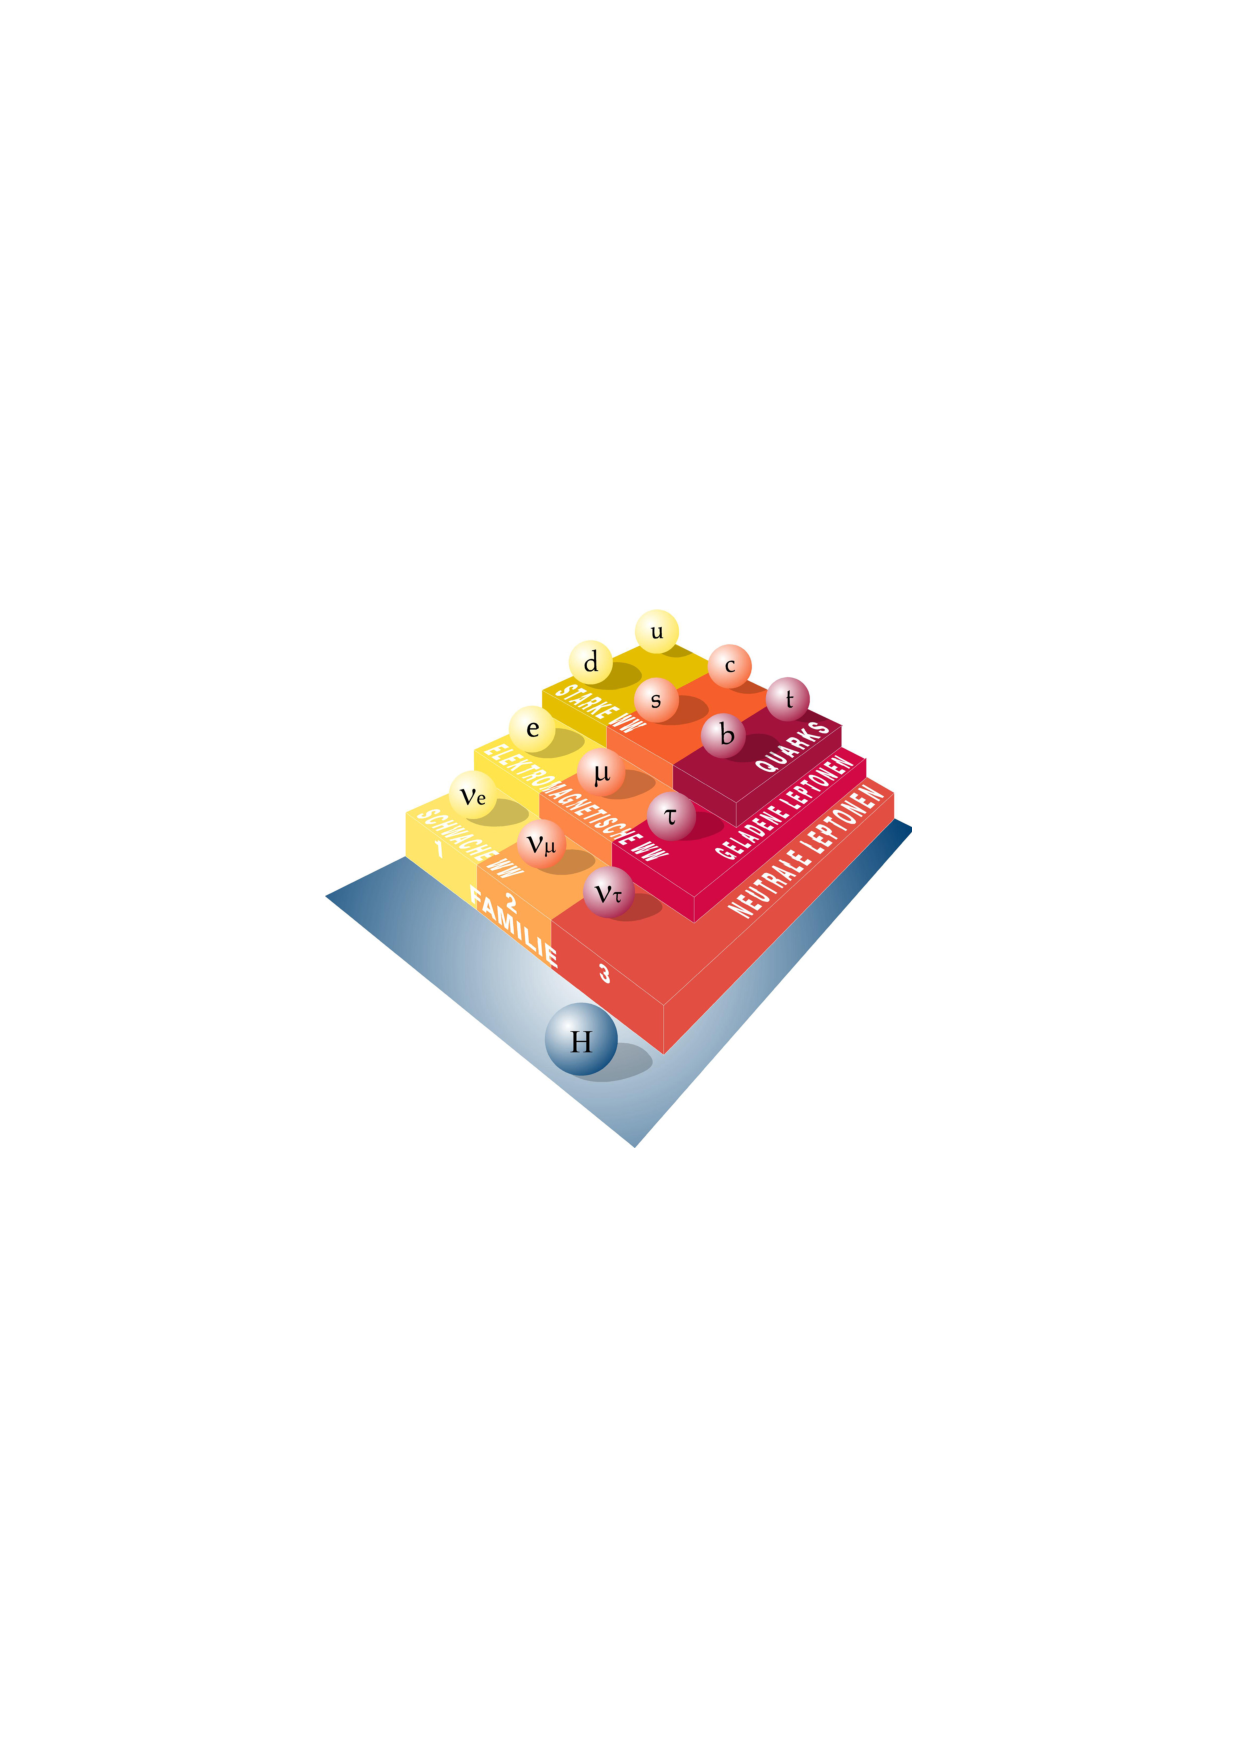
\includegraphics[width=0.5\textwidth]{fig/SM_teilchen.pdf}
	\caption{Fermionen des Standardmodells der Teilchenphysik und auf sie wirkende Kräfte. \cite{SM_teilchen}}
	\label{fig:SM_teilchen} 
\end{figure}\\
Sowohl die Quarks als auch die Leptonen sind in drei Familien unterteilt, wobei jede Familie einem Teilchenduplett entspricht. Bei den Quarks unterscheidet man weiter zwischen Up- und  Down-Type Quarks. Die Up-Type Quarks sind das up- ($\uquark$), charm- ($\cquark$) und top-Quark ($\tquark$), zu den Down-Type-Quarks gehören das down- ($\dquark$), strange- ($\squark$) und bottom-Quark ($\bquark$). Die Up-Type-Quarks tragen eine Ladung von $+\tfrac{2}{3}\electron$, während die Down-Type-Quarks eine Ladung von $-\tfrac{1}{3}\electron$ haben.\\
Bei den Leptonen unterscheidet man zwischen den geladenen Leptonen, dem Elektron ($\en$), dem Myon ($\mun$) und dem Tauon ($\taum$), und den ungeladenen Leptonen, den zugehörigen Neutrinos ($\neue$, $\neum$, $\neut$). Zu jedem dieser zwölf Fermionen gibt es ein zugehöriges Antiteilchen mit umgekehrter Ladung. Bei den Quarks spricht man bei dieser Unterscheidung auch vom sogenannten Flavour.\\
Zu den Bosonen gehören unter anderem die Eichbosonen, die direkt mit den im SM beschriebenen Kräften assoziiert sind. Die acht Gluonen $g$ sind Austauschteilchen der starken Wechselwirkung (WW) und koppeln an die  sogenannte Farbladung. Diese wird von Quarks getragen, die neben ihrer elektrischen Ladung eine Farbladung tragen. Die möglichen Farben sind grün, blau und rot, außerdem gibt es zu jeder Farbe auch eine Antifarbe. Teilchen mit Farbladungen können nicht frei auftreten, sondern müssen immer in gebundenen farbneutralen Zuständen existieren. So treten die Quarks immer in gebunden Zuständen von drei Quarks (Baryonen) mit drei Farben oder drei Antifarben oder in gebundenen Zuständen von zwei Quarks (Mesonen) mit einer Farbe und ihrer Antifarbe auf. Weil von den Fermionen nur die Quarks eine Farbladung tragen, sind diese als einzige Teilchen von der starken WW beeinflusst. Die Gluonen sind masselos und können, da sie eine Farbe und eine Antifarbe tragen, auch an sich selbst koppeln.\\ 
Als zweite WW wird die elektromagnetische WW beschrieben. Diese wird durch das Photon $\g$ vermittelt, das an die elektrische Ladung koppelt , sodass hier die Neutrinos als einzige elementare, ungeladene Fermionen nicht beeinflusst sind. Das Photon ist wie die Gluonen masselos, da es aber auch keine elektrische Ladung trägt, koppelt es nicht an sich selbst.\\ 
Die dritte WW im Standardmodell ist die schwache WW. Ihre Austauschteilchen sind das ungeladene \Z-Boson und die geladenen \Wpm-Bosonen. Im Gegensatz zu den bisher genannten Eichbosonen verfügen diese über Massen von $M_W\approx\SI{80}{GeV}$ und $M_Z\approx\SI{91}{GeV}$ \cite{PDG-2012}. Sie koppeln an alle der zwölf Fermionen.\\ 
Die schwache WW nimmt jedoch noch eine Sonderstellung ein. Sie koppelt an die linkshändigen Dupletts der Quarks und Leptonen. Bei den Leptonen können die Eigenzustände der schwachen WW unter Annahme von masselosen Neutrinos durch eine einfache Transformation in das Eigensystem der Masseneigenzustände der geladenen Leptonen überführt werden. Im Quarksektor ist dies jedoch nicht für beide Quarktypen möglich. Nach Konvention wählt man hier die Up-Type-Quarks, sodass man für die Down-Type-Quarks eine Transformationsmatrix $V_{C\!K\!M}$ zwischen den Eigenzuständen zur schwachen WW $\dquark'$, $\squark'$ und $\bquark'$ und den Masseneigenzuständen $\dquark$, $\squark$ und $\bquark$ erhält:
\begin{equation}
\begin{pmatrix}\dquark'\\ \squark'\\ \bquark'\end{pmatrix}=\begin{pmatrix}\Vud & \Vus & \Vub\\ \Vcd & \Vcs & \Vcb\\ \Vtd & \Vts & \Vtb\end{pmatrix}\begin{pmatrix}\dquark\\ \squark\\ \bquark\end{pmatrix}\approx\begin{pmatrix}1-\frac{\lambda^2}{2} & \lambda & A\lambda^3(\rho-i\eta)\\-\lambda & 1-\frac{\lambda^2}{2} & A\lambda^2\\A\lambda^3(1-\rho-i\eta) & -A\lambda^2 & 1\end{pmatrix}\begin{pmatrix}\dquark\\ \squark\\ \bquark\end{pmatrix}\label{eq:wolfen}
\end{equation}
Diese sogenannte $C\!K\!M$-Matrix hat vier Freiheitsgrade und ist unitär. Sie lässt sich, wie in Gleichung \eqref{eq:wolfen} dargestellt, mit der Wolfenstein Parametrisierung durch drei reelle Parameter ($A$, $\rho$, $\lambda$) und eine komplexe Phase ($\eta$) mit $\lambda\approx0{,}22$ parametrisieren \cite{ckm_param}. Man erkennt, dass die Matrixelemente bei größerer Entfernung von der Diagonalen kleiner werden.\\ 
Als letztes Eichboson gibt es im SM das erst vor kurzem entdeckte Higgs-Boson $\PH$ \cite{higgs_found,higgs_atlas}. Dieses ist Austauschteilchen des Higgs-Feldes und wechselwirkt mit allen massiven Teilchen. Das Higgs-Boson selbst hat eine Masse von $M_H\approx\SI{126}{GeV}$ \cite{PDG-2012}. 

\section{Symmetrien}\label{sec:disksym}

Man unterscheidet im SM zwischen diskreten Symmetrien und kontinuierlichen Eichsymmetrien. Bei den kontinuierlichen Eichsymmetrien wird dabei eine lokale Eichinvarianz gefordert, bei der in den jeweiligen Symmetriegruppen $U(1)$ (elektromagnetische WW), $SU(2)$ (schwache WW) und $SU(3)$ (starke WW) die WW entstehen. Die Eichbosonen treten als Generatoren der jeweiligen Eichtransformationen auf. Dies soll hier für die $U(1)$ Gruppe gezeigt werden. Die Lagrangedichte 
\begin{equation}
\mathcal{L}=\overline{\psi}\left(i\slashed{\partial}-m\right)\psi-\frac{1}{4}F^{\mu\nu}F_{\mu\nu}-\underbrace{eQ\overline{\psi}\gamma^\mu\psi}_{j^\mu} A_\mu
\end{equation}
bleibt  unter den Transformationen
\begin{align}
\psi\rightarrow\psi'&=e^{-ieQ\theta(x)}\psi\\
A_\mu\rightarrow A_\mu'&=A_\mu+\partial_\mu\theta
\end{align}
invariant. Hier lässt sich nun das Eichfeld $A_\mu$ mit dem Photon identifizieren und man erkennt den Wechselwirkungsterm $j^\mu A_\mu$. Fordert man nun für die höheren Symmetriegruppen äquivalent lokale Eichtransformationen, so werden entsprechend die weiteren Eichbosonen erzeugt.\\
Neben diesen kontinuierlichen Symmetrien gibt es außerdem drei diskrete Symmetrien im Standardmodell der Teilchenphysik.
\begin{itemize}
\item Der Paritätsoperator $P$ beschreibt eine Raumspiegelung $P\psi(t,\vec{x})=\psi(t,-\vec{x})$. Der Operator ist unitär, es gilt also $P^\dagger=P^{-1}$.
\item Mit der Ladungskonjugation $C$ wechselt man zwischen einem Teilchen und seinem Antiteilchen. Die Bezeichnung als Ladungskonjugation ist hier etwas irreführend, da auch alle weiteren additiven Quantenzahlen wie die Baryonenzahlen von $C$ beeinflusst werden. Ebenso wie der Paritätsoperator ist auch $C$ unitär.
\item Die dritte diskrete Symmetrie ist die Zeitumkehr $T$. Diese dreht das Vorzeichen der zeitlichen Komponente $T\psi(t,\vec{x})=\psi(-t,\vec{x})$. Im Gegensatz zu den anderen beiden Operatoren ist er jedoch nicht unitär sondern antiunitär, es gilt also $T^2=1$.
\end{itemize}
Die Symmetrien sind sowohl einzeln als auch in Kombination mit jeweils einer weiteren Symmetrie ($P\!T$, $C\!T$, $C\!P$) von der schwachen WW gebrochen. Erst die Kombination \CPT aller drei Symmetrien ist erhalten. Daraus folgen für Teilchen und Antiteilchen gleiche Massen und Lebenszeiten.

\section[head={Mischung von \B-Mesonen},tocentry={Mischung von \B-Mesonen}]{Mischung von $\mathbf{\B}$-Mesonen}\label{sec:mixing}

Wie bereits in Kapitel \ref{sec:grundlagen} erläutert, sind für Quarks Masseneigenzustände und Eigenzustände der schwachen WW, auch Flavoureigenzustände, nicht identisch. Gleiches gilt für aus Quarks zusammengesetzte Teilchen wie $\B$-Mesonen. Betrachtet man nun das Zweiteilchensystem aus \Bz (\bquarkbar\dquark) und \Bzb (\bquark\dquarkbar), so erhält man die zeitliche Entwicklung dieses Systems aus der Schrödingergleichung
\begin{equation}
i\frac{d}{dt}\begin{pmatrix}\Bz\\ \Bzb\end{pmatrix}=\mathcal{H}\begin{pmatrix}\Bz\\ \Bzb\end{pmatrix}=\left(M-\frac{i}{2}\Gamma\right)\begin{pmatrix}\Bz\\ \Bzb\end{pmatrix},
\end{equation}
wobei $M$ und $\Gamma$ hermitesche Matrizen sind. Aufgrund des $\CPT$-Theorems muss außerdem  $m_{11}=m_{22}$ und $\Gamma_{11}=\Gamma_{22}$ gelten. Diagonalisiert man diese Matrix nun erhält man die Eigenwerte $\mu_{1,2}=m_{1,2}-\frac{i}{2}\Gamma_{1,2}$ mit den Massen $m_{1,2}$ und Zerfallsbreiten $\Gamma_{1,2}$ der Masseneigenzustände. Im $\B$-System bezeichnet man  die Masseneigenzustände mit $\B_L$ und $\B_H$ und analog die zugehörigen Massen mit  $m_L$ und $m_H$ sowie die Zerfallsbreiten mit $\Gamma_L$ und $\Gamma_H$. Die Masseneigenzustände ergeben sich dabei zu
\begin{equation}
\begin{split}
\left|B_H\right>&\sim p\left|\Bz\right>-q\left|\Bzb\right>\\
\left|B_L\right>&\sim p\left|\Bz\right>+q\left|\Bzb\right>
\end{split}
\end{equation}
wobei $p$ und $q$ der Normierungsbedingung $\left|p\right|^2+\left|q\right|^2=1$ folgen müssen. Weiterhin lassen sich die Größen 
\begin{align}
\dm&=m_H-m_L\\
\Delta\Gamma&=\Gamma_H-\Gamma_L
\end{align}
definieren, wobei die Massendifferenz $\dm$ als positiv definiert ist. Für die Zeitentwicklung der Flavoureigenzustände erhält man 
\begin{equation}
\begin{split}
\left|\Bz(t)\right>&=\frac{1}{2}\left|\Bz\right>g_+-\frac{q}{2p}\left|\Bzb\right>g_-,\\
\left|\Bzb(t)\right>&=\frac{1}{2}\left|\Bzb\right>g_--\frac{p}{2q}\left|\Bz\right>g_+
\end{split}
\end{equation}
mit $g_\pm=e^{-\mu_Ht}\pm e^{-\mu_Lt}$. Nun lässt sich die Wahrscheinlichkeit berechnen, mit der ein produziertes ($t=0$) $\Bz$-Meson nach einer Zeit $t$ in ein $\Bzb$-Meson oszilliert ist:
\begin{equation}
\left|\left<\Bzb\Big|\Bz(t)\right>\right|^2=\frac{1}{4}\left|\frac{q}{p}\right|^2\left(e^{-\Gamma_Ht}+e^{-\Gamma_Lt}-2e^{\frac{1}{2}\left(\Gamma_H+\Gamma_L\right)t}\cos\left(\dm t\right)\right).\label{eq:uebergang1}
\end{equation}
Man erkennt, dass die Wahrscheinlichkeit eines anfänglichen $\Bz$-Mesons als $\Bzb$-Meson zu zerfallen, mit der Frequenz $\dm$ oszilliert. Ebenso lässt sich die Wahrscheinlichkeit für ein anfängliches $\Bzb$-Meson definieren. Die Feynmangraphen zu beiden Prozessen sind in Abbildung \ref{fig:mixing} zu sehen.\\
Analog zu Gleichung \eqref{eq:uebergang1} lassen sich die Wahrscheinlichkeiten $\left|\left<\Bz\Big|\Bzb(t)\right>\right|^2$, $\left|\left<\Bzb\Big|\Bzb(t)\right>\right|^2$ und $\left|\left<\Bz\Big|\Bz(t)\right>\right|^2$ berechnen:
\begin{align}
\left|\left<\Bz\Big|\Bzb(t)\right>\right|^2&=\frac{1}{4}\left|\frac{p}{q}\right|^2\left(e^{-\Gamma_Ht}+e^{-\Gamma_Lt}-2e^{\frac{1}{2}\left(\Gamma_H+\Gamma_L\right)t}\cos\left(\dm t\right)\right),\label{eq:uebergang2}\\
\left|\left<\Bzb\Big|\Bzb(t)\right>\right|^2&=\frac{1}{4}\left(e^{-\Gamma_Ht}+e^{-\Gamma_Lt}+2e^{\frac{1}{2}\left(\Gamma_H+\Gamma_L\right)t}\cos\left(\dm t\right)\right),\label{eq:uebergang3}\\
\left|\left<\Bz\Big|\Bz(t)\right>\right|^2&=\frac{1}{4}\left(e^{-\Gamma_Ht}+e^{-\Gamma_Lt}+2e^{\frac{1}{2}\left(\Gamma_H+\Gamma_L\right)t}\cos\left(\dm t\right)\right).\label{eq:uebergang4}
\end{align}
Ohne $\CP$-Verletzung in der Mischung (siehe Abschnitt \ref{sec:cpv}) lässt sich eine Mischungsasymmetrie berechnen:
\begin{equation}
\begin{split}
A_{\text{mix}}(t)&=\frac{\left(\Gamma(\Bz(t)\rightarrow\Bz)+\Gamma(\Bzb(t)\rightarrow\Bzb)\right)-\left(\Gamma(\Bzb(t)\rightarrow\Bz)+\Gamma(\Bz(t)\rightarrow\Bzb)\right)}{\left(\Gamma(\Bz(t)\rightarrow\Bz)+\Gamma(\Bzb(t)\rightarrow\Bzb)\right)+\left(\Gamma(\Bzb(t)\rightarrow\Bz)+\Gamma(\Bz(t)\rightarrow\Bzb)\right)}\\
&=\frac{N_\text{unmixed}(t)-N_\text{mixed}(t)}{N_\text{unmixed}(t)+N_\text{mixed}(t)}=\cos(\dm t).\label{eq:mixing}
\end{split}
\end{equation}
Dabei ist $N_\text{unmixed}(t)$ die Anzahl der nicht oszillierten $\B$-Mesonen und $N_\text{mixed}(t)$ die Anzahl der oszillierten $\B$-Mesonen zum Zeitpunkt $t$. Für  \Bz-Mesonen gilt außerdem $\Gamma_H\approx\Gamma_L$.
\begin{figure}[htbp]
	\begin{center}
		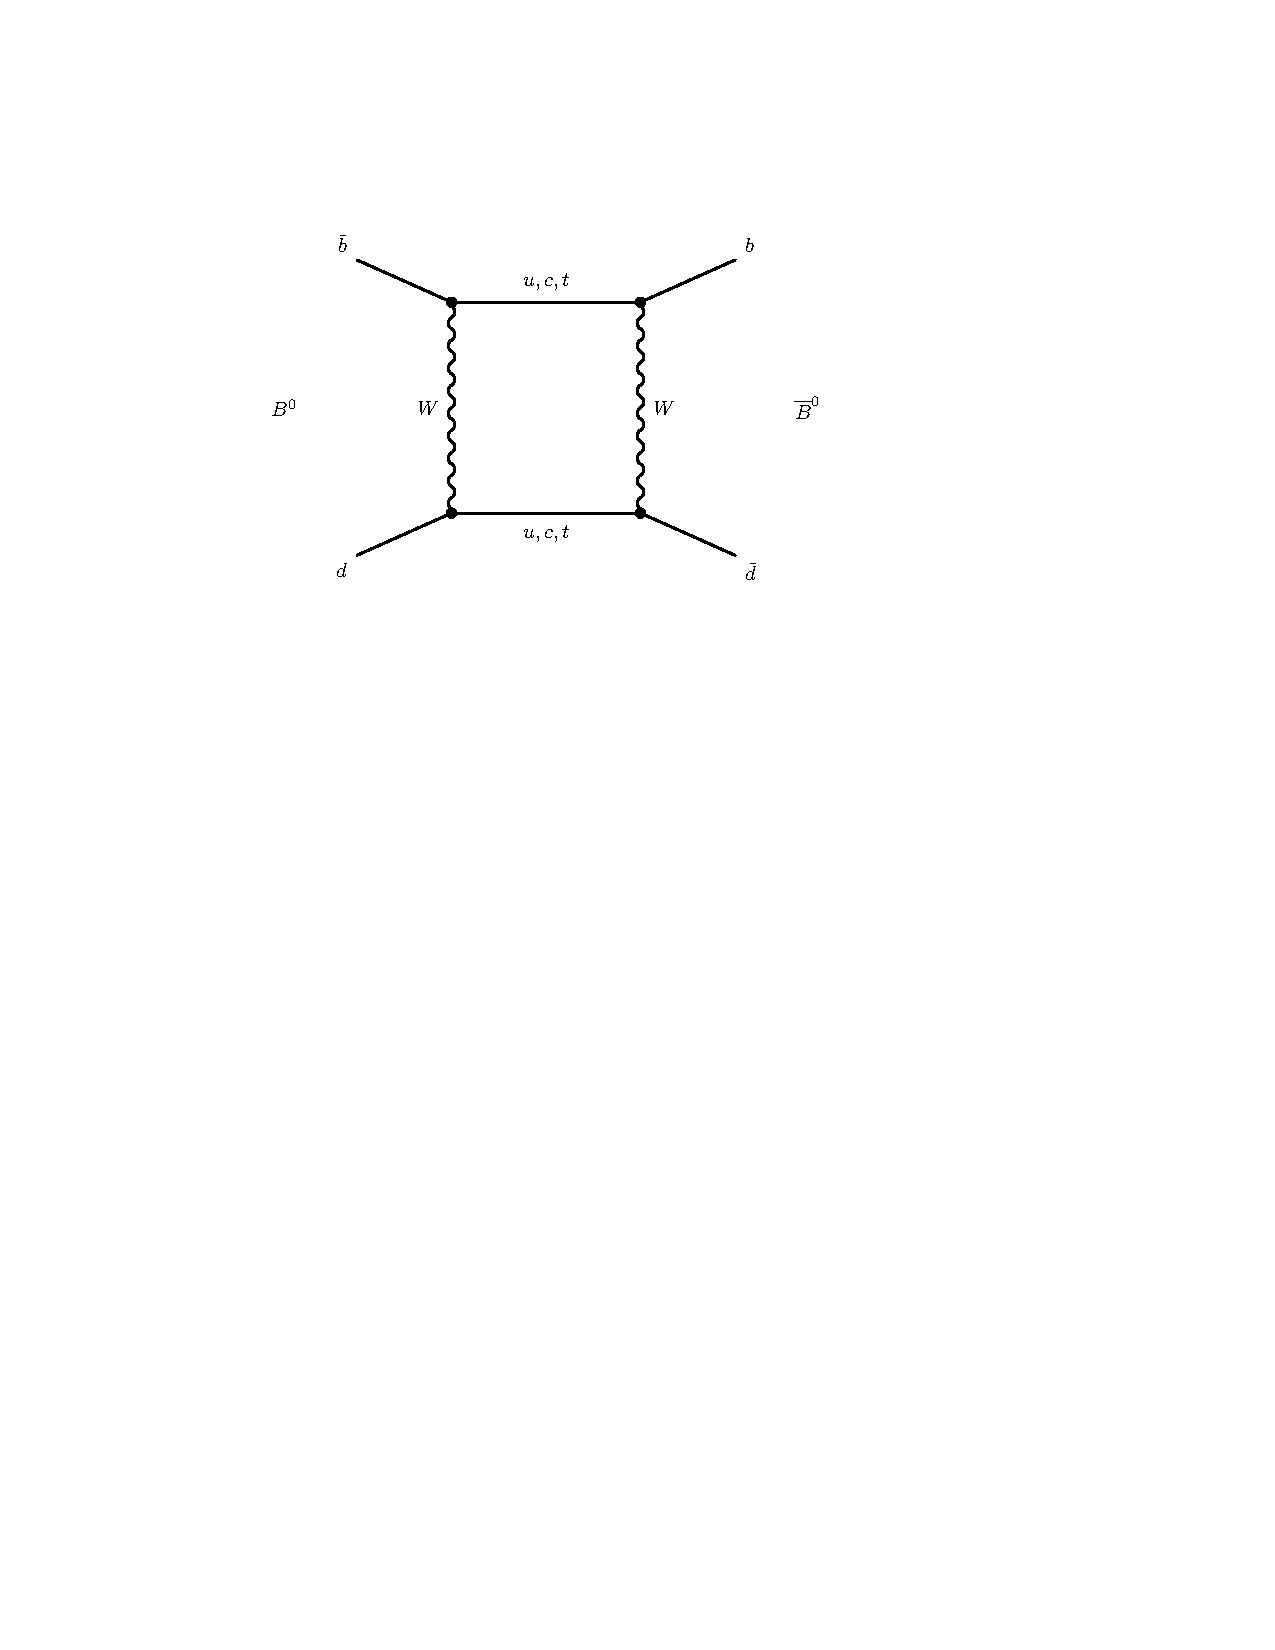
\includegraphics[width=0.45\textwidth]{fig/B_mixing_1.pdf}
		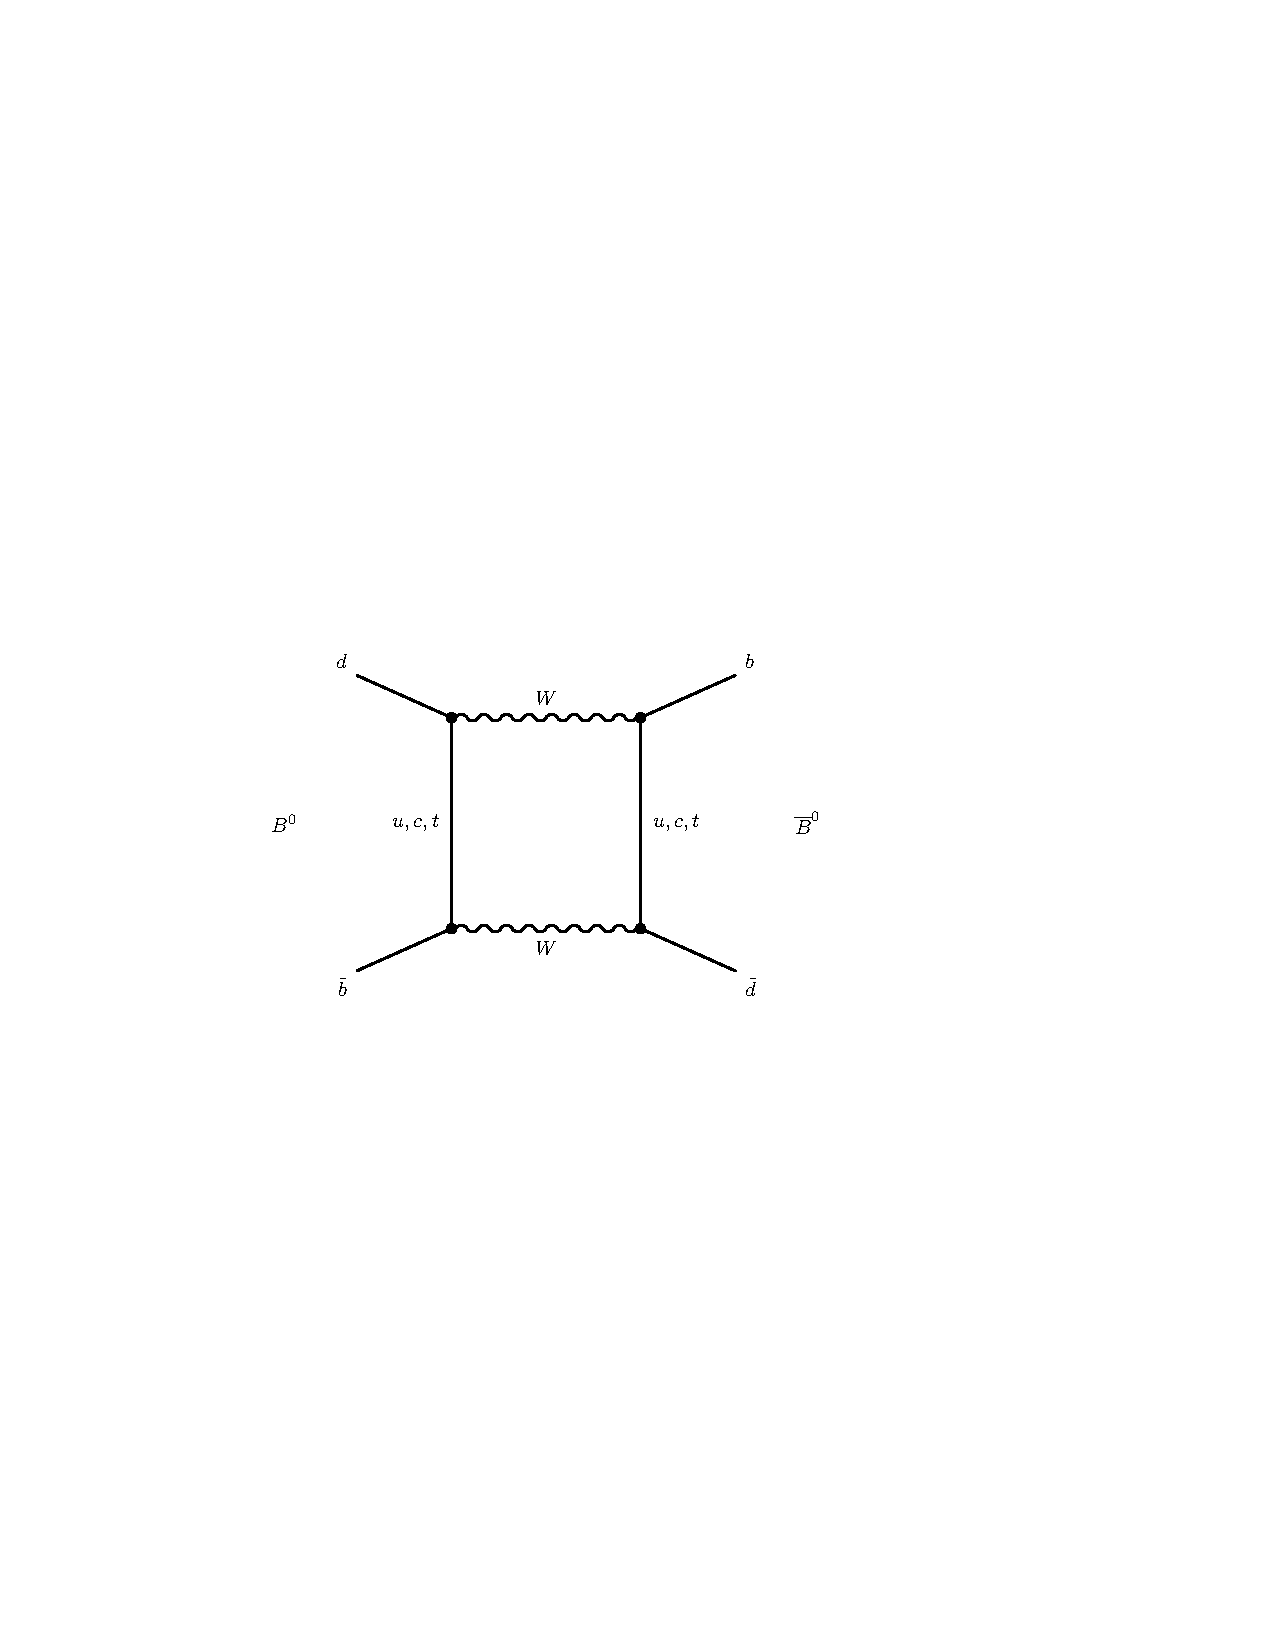
\includegraphics[width=0.45\textwidth]{fig/B_mixing_2.pdf}
	\caption{Box-Diagramme niedrigster Ordnung zur Oszillation neutraler \Bz-Mesonen. Dominiert werden beide Diagramme vom $\tquark$-Quark.}
	\label{fig:mixing}
 	\end{center}
\end{figure}

\section[head={$\CP$-Verletzung},tocentry={$\CP$-Verletzung}]{$\mathbf{CP}$-Verletzung}\label{sec:cpv}

Die $\CP$-Symmetrie ist, wie in Kapitel \ref{sec:disksym} angemerkt, von der schwachen WW gebrochen. Um zwischen den verschiedenen Arten der $\CP$-Verletzung zu unterscheiden, sollen zunächst vier Zerfallsamplituden eingeführt werden
\begin{equation}
\begin{split}
A_f=\left<f\big|T\big|\Bz\right>&\hspace{1.5cm}\overline{A}_f=\left<f\Big|T\Big|\Bzb\right>\\
A_{\bar{f}}=\left<\bar{f}\Big|T\Big|\Bz\right>&\hspace{1.5cm}\overline{A}_{\bar{f}}=\left<\bar{f}\Big|T\Big|\Bzb\right>,
\end{split}
\end{equation}
wobei $T$ die Übergangsmatrix zwischen dem $\B$-Meson und einem beliebigen Endzustand $f$ darstellt. Nun lässt sich zwischen drei Arten von $\CP$-Verletzung unterscheiden:
\begin{itemize}
\item Direkte $\CP$-Verletzung, oder auch $\CP$-Verletzung im Zerfall, bedeutet, dass sich die Zerfallsamplituden zwischen $\Bz$ und $\Bzb$-Meson unterscheiden. Es gilt also $\left|A_f\right|\neq\left|\overline{A}_{\bar{f}}\right|$ und $\left|A_{\bar{f}}\right|\neq\left|\overline{A}_f\right|$
\item Bei der indirekten $\CP$-Verletzung ($\CP$-Verletzung in der Mischung) sind die Übergangswahrscheinlichkeiten von $\Bz$ nach $\Bzb$ und andersherum voneinander verschieden. Für die Matrixelemente bedeutet dies, dass $\left|\left<\Bzb\Big|\Bz(t)\right>\right|\neq\left|\left<\Bz\Big|\Bzb(t)\right>\right|$ und damit $\left|\tfrac{q}{p}\right|\neq1$. 
\item Die dritte Art der $\CP$-Verletzung kann in der Interferenz von Mischung und Zerfall auftreten. Im einfachsten Fall zerfallen beide Flavoureigenzustände in einen gemeinsamen Endzustand. Allgemein gilt für diese Art der $\CP$-Verletzung $\left<f\big|T\big|\Bz(t)\right>\neq\left<\bar{f}\Big|T\Big|\Bzb(t)\right>$. Betrachtet man nun die Größe
\begin{equation}
\lambda_f=\frac{q}{p}\frac{\overline{A}_f}{A_f}
\end{equation}
lässt sich dies umformulieren. Selbst ohne direkte oder indirekte $\CP$-Verletzung ($\lambda_f=\pm1$), kann $\mathcal{Im}(\lambda_f)\neq0$ gelten und damit $\CP$-Verletzung in der Interferenz aus Mischung und Zerfall auftreten. 
\end{itemize}
Im Standardmodell ist die $\CP$-Verletzung in der komplexen Phase der $C\!K\!M$-Matrix verankert: Da die schwache Wechselwirkung nicht an die Flavoureigenzustände koppelt, ist es so möglich, dass es zwischen Teilchen und Antiteilchen zu den beschriebenen Asymmetrien kommt. Aus der Unitarität der $C\!K\!M$-Matrix folgen die Gleichungen 
\begin{equation}
\sum_{i}V_{ij}V_{ik}^*=\delta_{jk} \hspace{0.5cm}\text{ und }\hspace{0.5cm} \sum_{j}V_{ij}V_{kj}^*=\delta_{ik}.
\end{equation}
Diese Gleichungen lassen sich als Dreiecke in der komplexen Ebene darstellen, deren Fläche ein Maß für die Größe der \CP-Verletzung ist. Die gebräuchlichste dieser Gleichungen ist
\begin{equation}
\Vud\Vubst+\Vcd\Vcbst+\Vtd\Vtbst=0.
\end{equation}
Normiert man diese Gleichung auf das Produkt $\Vcd\Vcb^*$ erhält man das in Abbildung \ref{fig:ckm} darstgestellte Dreieck: 
\begin{equation}
\frac{\Vud\Vubst}{\Vcd\Vcbst}+1+\frac{\Vtd\Vtbst}{\Vcd\Vcbst}=0.
\end{equation}
\begin{figure}[htbp]
	\begin{center}
		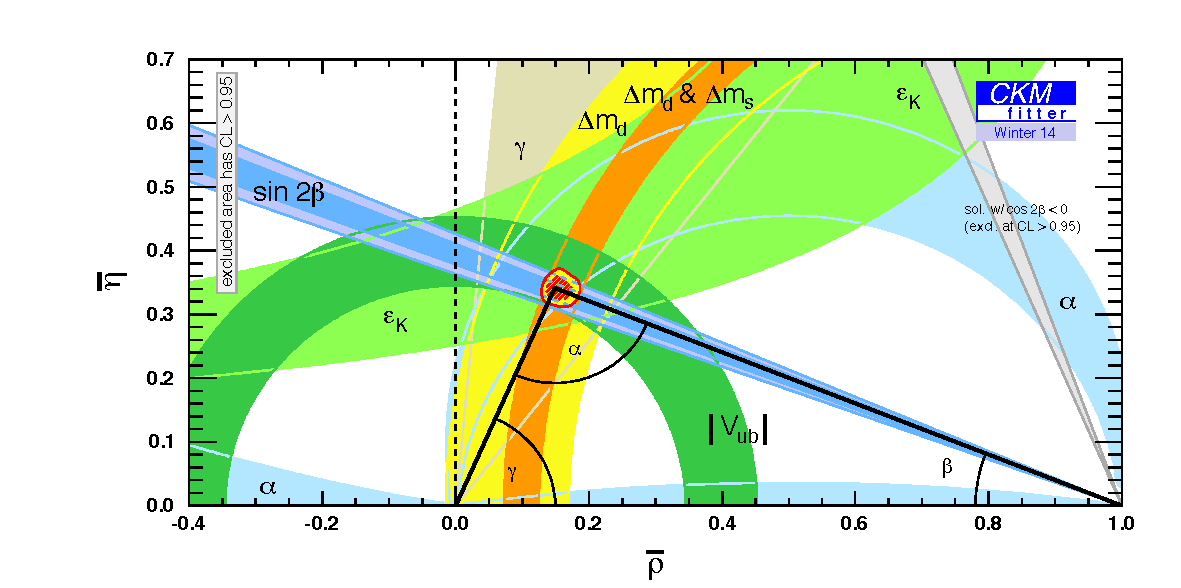
\includegraphics[width=0.65\textwidth]{fig/ckm_fitter.pdf}
	\caption{$C\!K\!M$-Dreieck in der komplexen Ebene. Die farbigen Bänder markieren die Unsicherheiten auf verschiedene Parameter des Dreiecks.\cite{ckm-fitter}}
	\label{fig:ckm}
 	\end{center}
\end{figure}
Bei einer verschwindenden komplexen Phase in der Matrix, also ohne $\CP$-Verletzung, würde die Spitze des Dreiecks auf der reellen Achse liegen, und dieses zu einer Linie entarten.\\ 
In der modernen Teilchenphysik sind diese $C\!K\!M$-Dreiecke von großer Bedeutung. Durch Ausmessen verschiedener Größen der Dreiecke lassen sie sich überbestimmen. Sollten nun experimentelle Daten zeigen, dass ein solches Dreieck nicht schließt, wäre dies ein Hinweis auf Physik jenseits des SM.\\
Im Folgenden soll nun speziell das System der $\Bz$-Mesonen betrachtet werden. Neben der in Abschnitt \ref{sec:mixing} beschriebenen Mischungsasymmetrie lässt sich auch eine $\CP$-Asymmetrie definieren. Dafür wird zunächst die Übergangswahrscheinlichkeit $\left|\left<f\big|T\big|\Bz(t)\right>\right|^2$ berechnet, wobei $\Bz(t)$ ein \B-Meson beschreibt das bei $t=0$ als \Bz erzeugt worden ist ($\Gamma_H\approx\Gamma_L$ für \Bz und \Bzb):
\begin{align}
\left|\left<f\big|T\big|\Bz(t)\right>\right|^2&=\left|\frac{1}{2}\left<f\big|T\big|\Bz\right>g_+-\frac{q}{2p}\left<f\Big|T\Big|\Bzb\right>g_-\right|^2\nonumber\\
&=\frac{1}{4}A_f^2\left|g_+-\frac{q}{p}\frac{\overline{A}_f}{A_f}g_-\right|^2=\frac{1}{4}A_f^2\left|g_+-\lambda_fg_-\right|^2\nonumber\\
&=\frac{1}{4}A_f^2\left(g_+g_+^*+\left|\lambda_f\right|^2g_-g_-^*-\overline{\lambda_f}g_+g_-^*-\lambda_f g_+^*g_-\right)\nonumber\\
&=\frac{1}{2}A_f^2e^{-\Gamma t}\left[\left(1+\left|\lambda_f\right|^2\right)+\left(1-\left|\lambda_f\right|^2\right)\cos\left(\dm t\right)-2\mathcal{Im}\left(\lambda_f\right)\sin\left(\dm t\right)\right]
\end{align}
Analog dazu erhält man
\begin{align}
\left|\left<\overline{f}\Big|T\Big|\Bzb(t)\right>\right|^2&=\frac{1}{2}A_f^2e^{-\Gamma t}\left[\left(1+\left|\lambda_f\right|^2\right)-\left(1-\left|\lambda_f\right|^2\right)\cos\left(\dm t\right)+2\mathcal{Im}\left(\lambda_f\right)\sin\left(\dm t\right)\right]\\
\left|\left<\overline{f}\Big|T\Big|\Bz(t)\right>\right|^2&=\frac{1}{2}A_f^2e^{-\Gamma t}\left[\left(1+\left|\lambda_f\right|^2\right)-\left(1-\left|\lambda_f\right|^2\right)\cos\left(\dm t\right)-2\mathcal{Im}\left(\lambda_f\right)\sin\left(\dm t\right)\right]\\
\left|\left<f\Big|T\Big|\Bzb(t)\right>\right|^2&=\frac{1}{2}A_f^2e^{-\Gamma t}\left[\left(1+\left|\lambda_f\right|^2\right)+\left(1-\left|\lambda_f\right|^2\right)\cos\left(\dm t\right)+2\mathcal{Im}\left(\lambda_f\right)\sin\left(\dm t\right)\right].
\end{align}
Mit diesen Übergangswahrscheinlichkeiten ergibt sich die $\CP$-Asymmetrie zu:
\begin{equation}
A_\CP=\frac{\Gamma\left(\Bzb(t)\rightarrow f_\CP\right)-\Gamma\left(\Bz(t)\rightarrow f_\CP\right)}{\Gamma\left(\Bzb(t)\rightarrow f_\CP\right)+\Gamma\left(\Bz(t)\rightarrow f_\CP\right)}=\frac{2\mathcal{Im}(\lambda_f)}{1+\left|\lambda_f\right|^2}\sin\left(\dm t\right).\label{eq:cpv}
\end{equation}
Dabei ist $\frac{2\mathcal{Im}(\lambda_f)}{1+\left|\lambda_f\right|^2}$ die $\CP$-verletztende Größe, die hier mit $S_\CP$ bezeichnet werden soll und aus dem in Abbildung \ref{fig:ckm} gezeigten Dreieck den Winkel $\beta$ enthält: 
\begin{equation}
A_\CP=S_\CP\sin\left(\dm t\right)=\sin\left(2\beta\right)\sin\left(\dm t\right)
\end{equation}


  % !TEX root = main.tex
\chapter{Das \lhcb-Experiment}

Das $\lhcb$-Experiment ist neben $\atlas$, $\cms$ und $\alice$ eines der vier großen Experimente am europäischen Kernforschungszentrum $\cern$. Das Experiment ist auf Präzisionsmessungen der Physik von Prozessen mit $\bquark$- und $\cquark$-Quarks spezialisiert. Im Folgenden wird zunächst kurz auf den Large-Hadron-Collider ($\lhc$) eingegangen, um danach den $\lhcb$-Detektor und seine Komponenten detaillierter zu beschreiben (basierend auf \cite{Alves:2008zz}). Am Ende des Kapitels folgt ein Abschnitt über das LHCb Software Framework.

\section{Der $\lhc$}

\begin{figure}[htpb]
	\centering
		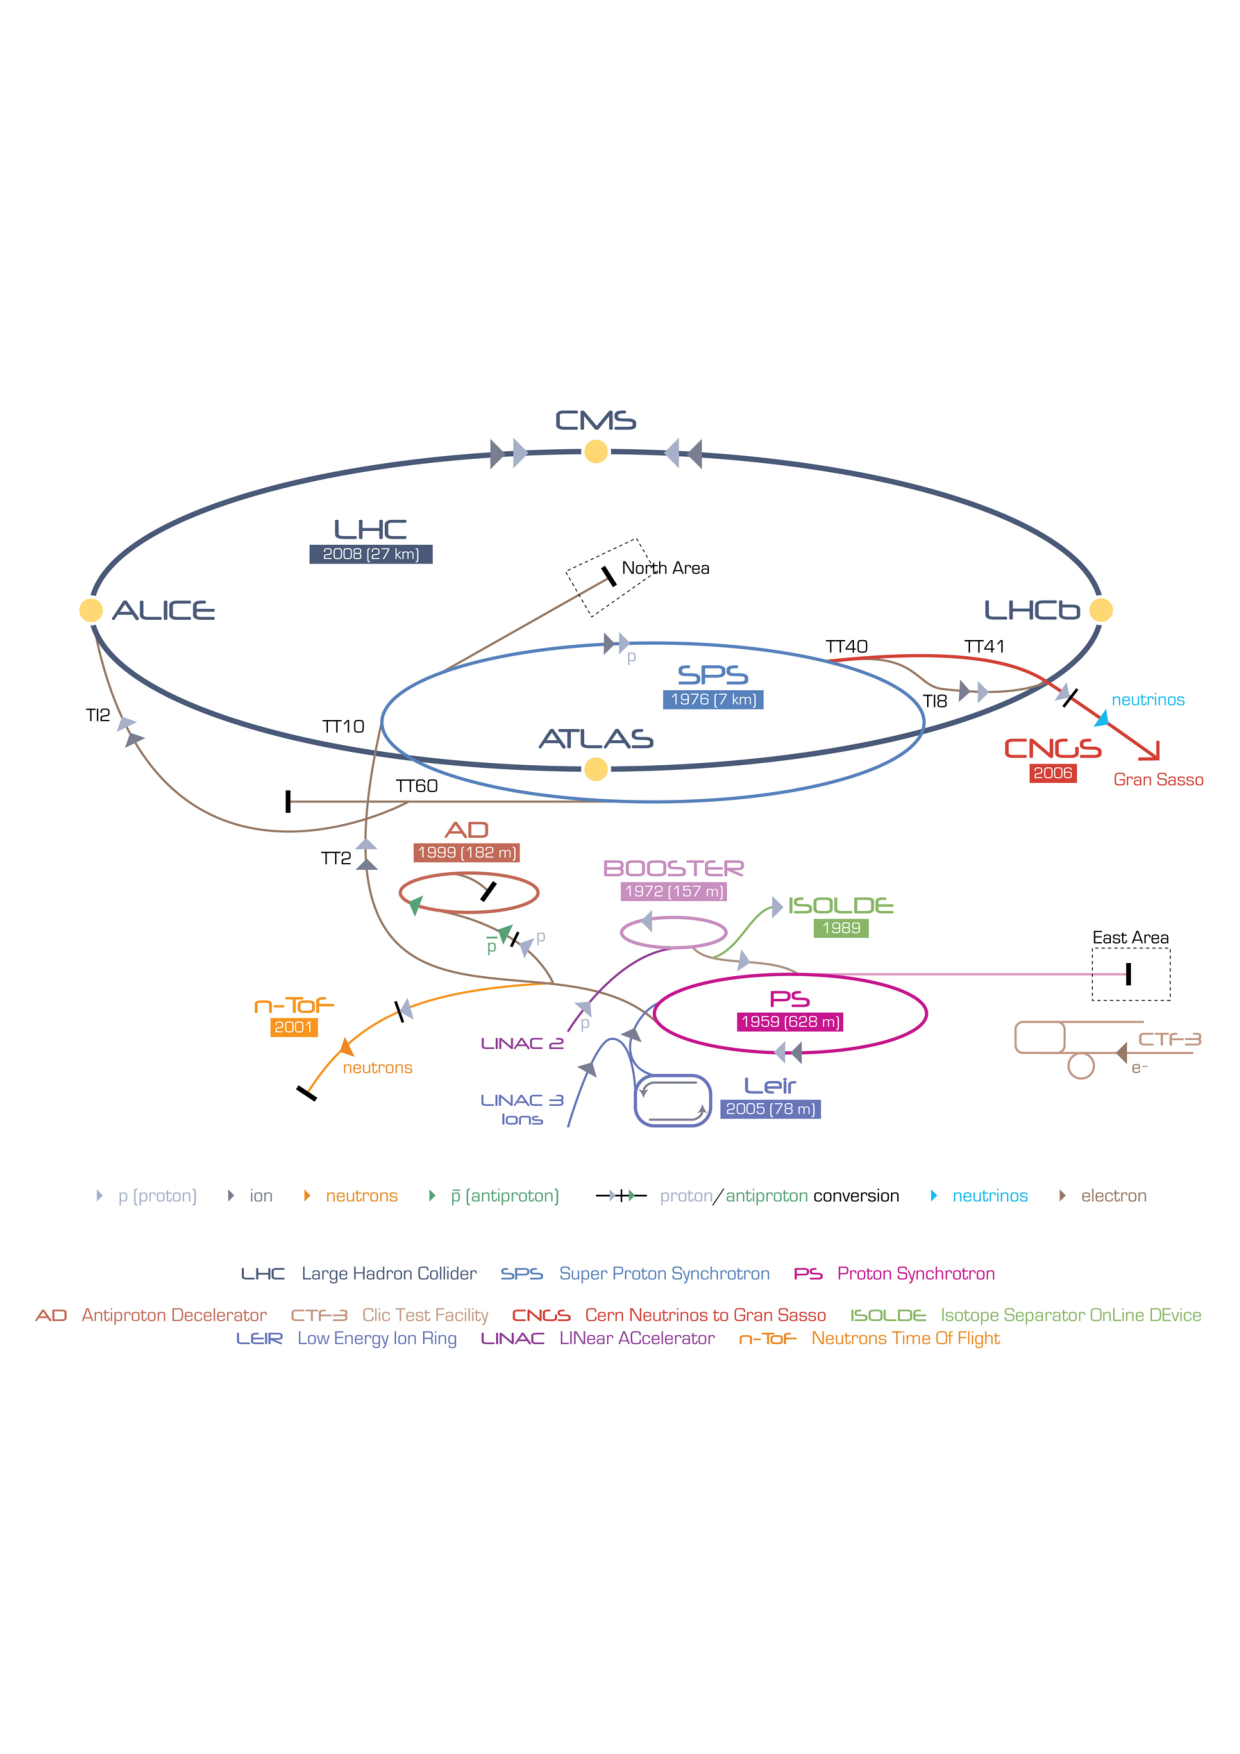
\includegraphics[width=0.75\textwidth]{fig/cern_scheme.pdf}
	\caption{Schematische Darstellung des $\cern$-Beschleuniger Komplexes. Die Protonen für den $\lhc$ werden zunächst im LINAC 2, im Booster, im Proton Synchrotron ($P\!S$) und im Super Proton Synchrotron ($S\!P\!S$) auf eine Energie von \SI{450}{GeV} vorbeschleunigt. Ihr Weg ist in der Abbildung durch die hellgrauen Pfeile gekennzeichnet \cite{cern_scheme}.}
	\label{fig:cern_scheme} 
\end{figure} 
Der $\lhc$ ist ein Ringbeschleuniger am $\cern$ bei Genf mit etwa \SI{27}{km} Umfang. Er ist dafür konstruiert, Protonen bei einer Schwerpunktsenergie von bis zu $\sqrt{s}=\SI{14}{TeV}$ bei einer Luminosität von \SI{e34}{cm^{-2}s^{-1}} \cite{lhc_design} kollidieren zu lassen. Dazu kreisen zwei entgegengesetzte Protonenstrahlen (Beams) im Beschleunigerring und werden an vier Punkten zur Kollision gebracht. \\
Bei den in dieser Arbeit verwendeten Daten bestanden die Beams aus etwa \num{1380} Protonen-Paketen, die jeweils \num{1{,}15e11} Protonen enthalten \cite{LHC_statistik}. Die Anzahl Pro\-tonen-Pakete pro Beam wird voraussichtlich nach dem Long-Shutdown $1$ ($L\!S1$) auf $2808$ \cite{lhc_design} gesteigert. \\
Bevor die Protonen in den $\lhc$-Beschleunigerring eingespeist werden, müssen sie vorbeschleunigt werden. Dies geschieht zunächst in einem Linearbeschleuniger, dem LINAC 2. Darauf folgen der Booster, das Proton-Synchrotron ($P\!S$) und das Super-Proton-Synchrotron ($S\!P\!S$) die allesamt Ringbeschleuniger sind. Aus dem $S\!P\!S$ werden die Protonen dann schließlich mit einer Energie von \SI{450}{GeV} \cite{lhc_design} in den $\lhc$-Ring eingespeist (Abbildung \ref{fig:cern_scheme}). Um die nahezu lichtschnellen Protonen auf ihrer kreisförmigen Bahn zu halten, sind  \num{1232}  supraleitende Dipolmagnete mit einer Länge von jeweils \SI{14{,}3}{m} und einer Feldstärke von bis zu \SI{8{,}33}{T} nötig. Die ersten Protonen im \lhc wurden im Jahr \num{2008} beschleunigt.\\
Insgesamt sind, wie bereits erwähnt, vier große Experimente am $\lhc$ in Betrieb. Bei $\atlas$ und $\cms$ handelt es sich dabei um Mehrzweckexperimente, die bei maximaler Luminosität experimentieren, $\alice$ untersucht vor allem Quark-Gluon-Plasmen. Das vierte Experiment, $\lhcb$, beschäftigt sich primär mit Präzisionsmessungen im Bereich der Flavour-Physik, vornehmlich mit $\bquark$- und $\cquark$-Hadronen. Im Gegensatz zu den drei anderen Experimenten deckt der Detektor auch nicht den gesamten Raumwinkel ab, sondern ist ein Vorwärts-Spektrometer.

\section{Der LHCb-Detektor}

Der $\lhcb$-Detektor ist ein Ein-Arm Vorwärts-Spektrometer mit einer Winkelabdeckung von etwa \SI{10}{mrad} bis etwa \SI{250}{mrad}. Die Detektorgeometrie ist damit begründet, dass die hauptsächlich untersuchten $\bbbar$-Quark Paare eine große Wahrscheinlichkeit dafür aufweisen in Vorwärts- oder Rückwärtsrichtung erzeugt zu werden (Abbildung \ref{fig:angle_plot}).  
\begin{figure}[htpb]
	\centering
		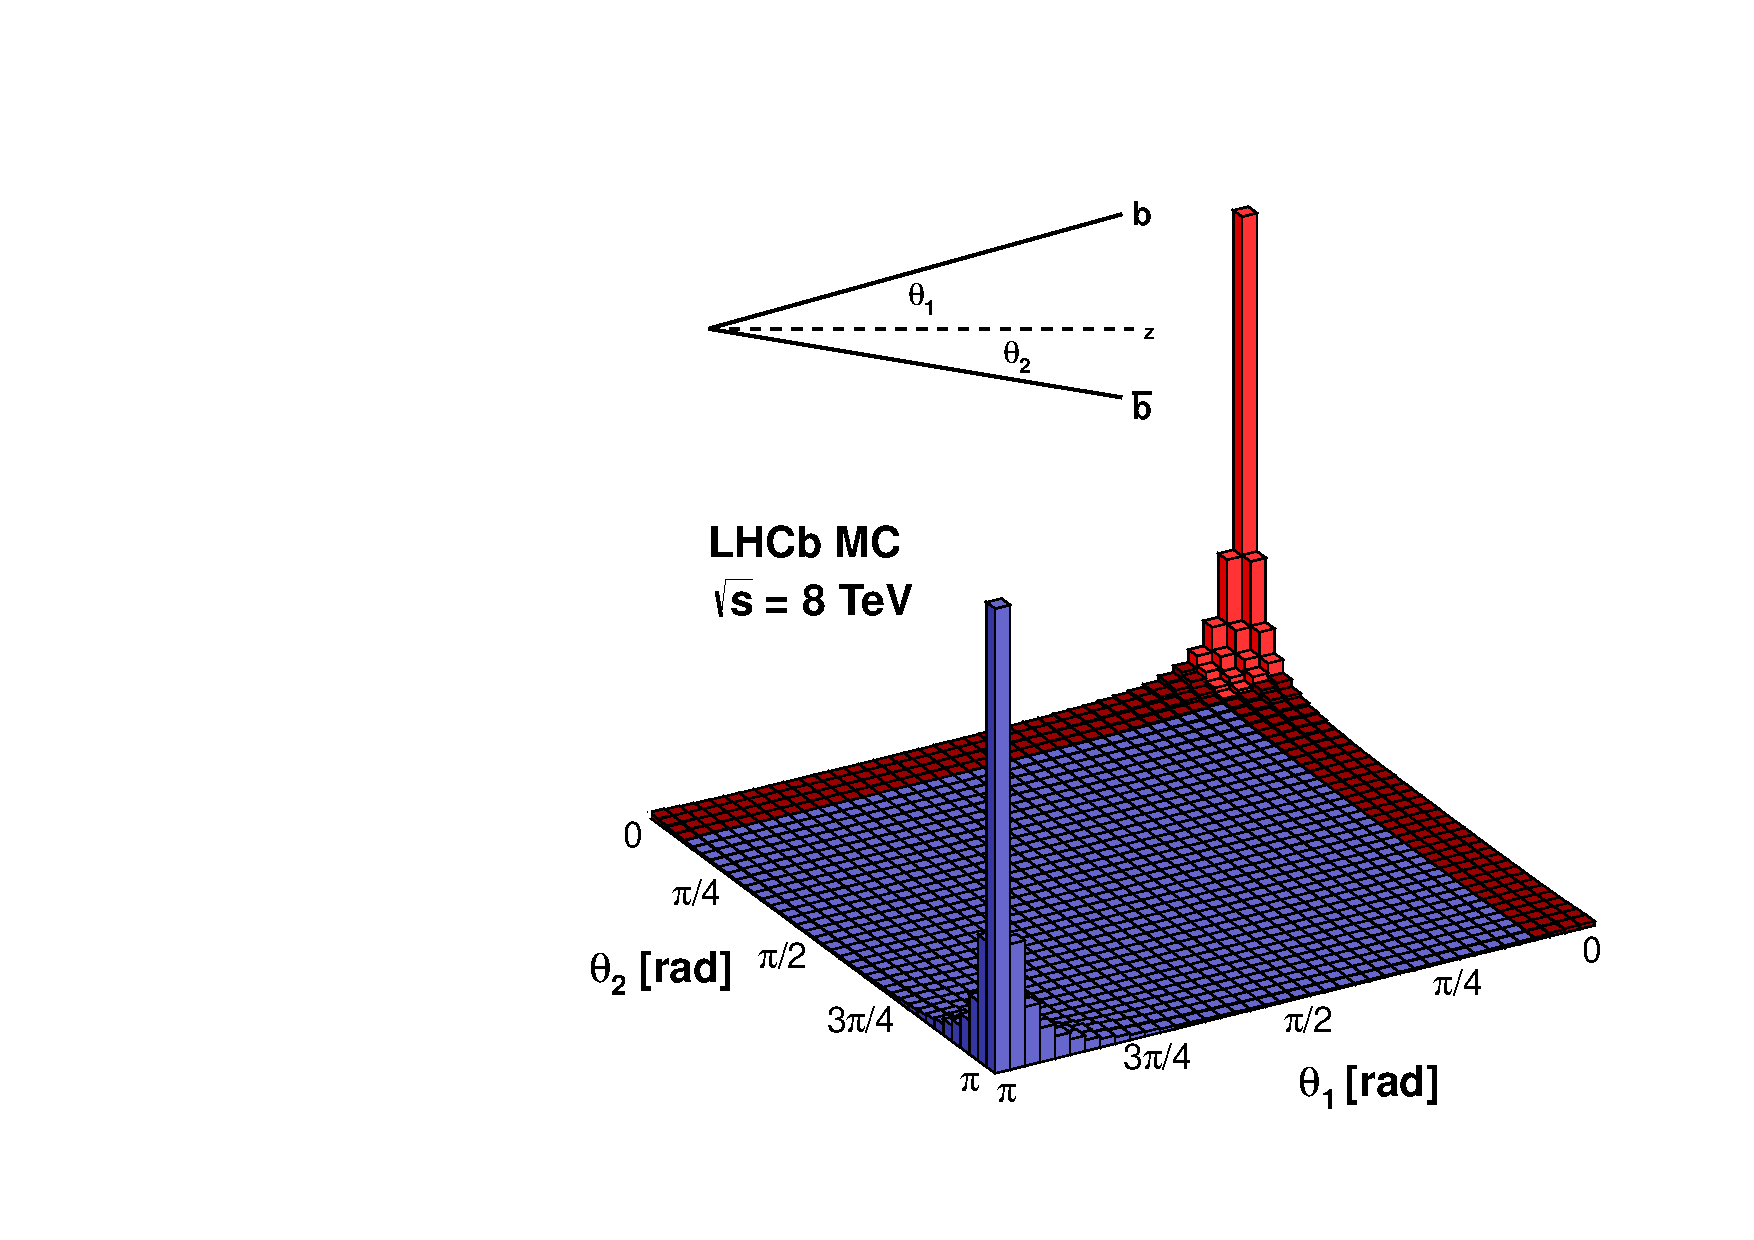
\includegraphics[width=0.5\textwidth]{fig/angle_plot.pdf}
	\caption{Winkelverteilung der $\bbbar$-Quark Paare zur Strahlachse bei einer Proton-Proton-Kollision. In rot ist der von \lhcb abgedeckte Winkelbereich dargestellt \cite{angle_plot}.}
	\label{fig:angle_plot} 
\end{figure} 
So liegen trotz der geringen Raumwinkelabdeckung etwa \SI{25}{\%} der $\bbbar$-Quark Paare innerhalb der Detektorakzeptanz. Weiterhin ist es bei $\lhcb$ wichtig, einzelne Prozesse möglichst detailliert aufzulösen. Dies ist umso einfacher, je weniger Proton-Proton-Kollisionen gleichzeitig stattfinden. Daher wird bei $\lhcb$ nicht die maximale vom $\lhc$ zur Verfügung gestellte Luminosität genutzt, sondern eine konstante Luminosität von etwa \SI[exponent-product = \cdot]{4e32}{cm^{-2}s^{-1}} \cite{LHC_statistik}. Diese wird eingestellt, indem der Überlapp der kollidierenden Protonenpakete bei $\lhcb$ kleiner ist als bei den anderen Experimenten. Da die Kollisionsrate mit aktuell \SI{20}{MHz} jedoch immer noch zu hoch ist, um alle Ereignisse direkt zu speichern, sind außerdem leistungsstarke Trigger vonnöten, die bereits eine erste Selektion der Daten vornehmen und möglichst viele Signalendzustände erhalten. Im Folgenden werden nun die einzelnen Komponenten des $\lhcb$-Detektors (Abbildung \ref{fig:det_plot}) in Anlehnung an \cite{Alves:2008zz}  erläutert.
\begin{figure}[htpb]
	\centering
		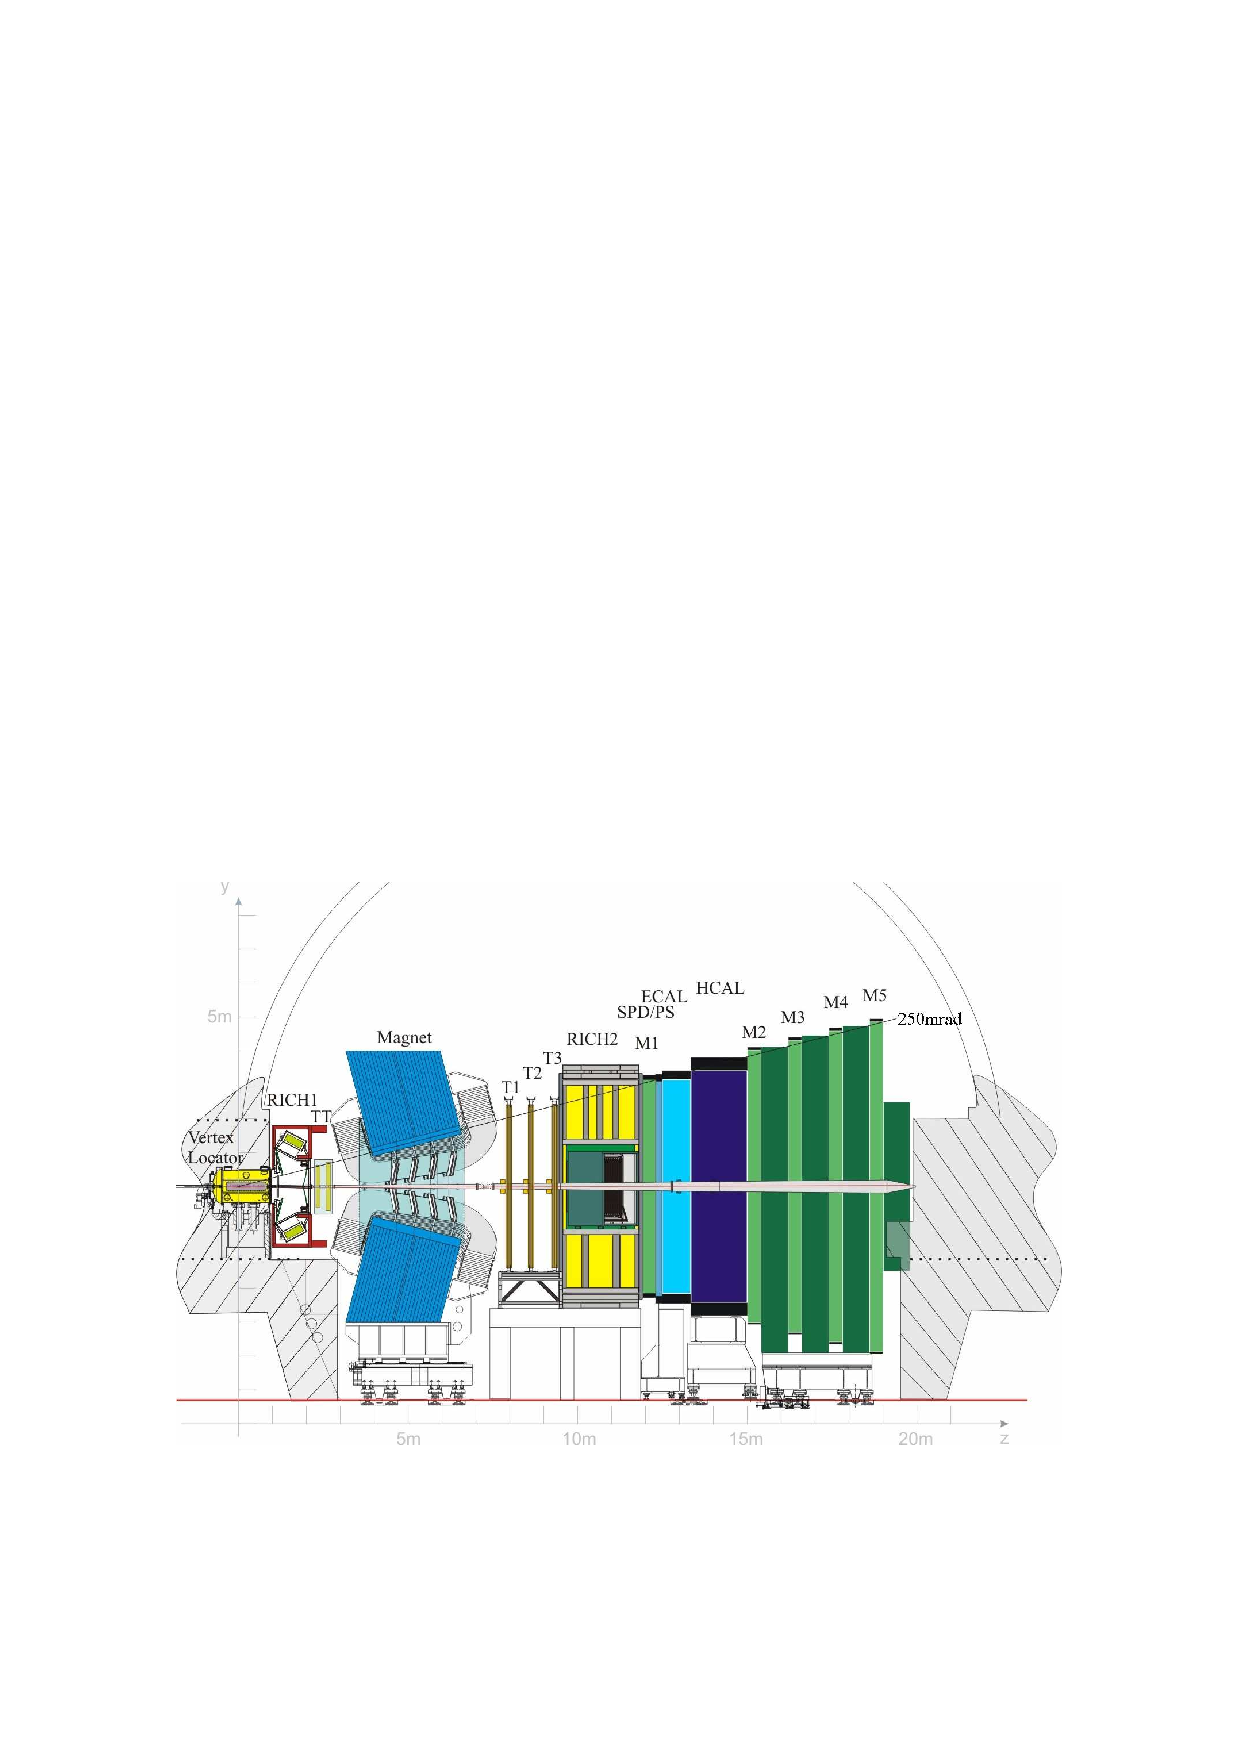
\includegraphics[width=0.8\textwidth]{fig/det_plot.pdf}
	\caption{Schematischer Aufbau des \lhcb-Detektors: Zu sehen sind der \velo, die beiden \rich-Detektoren, sowie das Tracking System mit Magnet, die Kalorimeter und die Myonenkammern. Der Kollisionspunkt wird links vom \velo umschlossen \cite{Alves:2008zz}.}
	\label{fig:det_plot} 
\end{figure} 

\subsection{Der Vertex-Locator}\label{sec:velo}

Der Vertex-Locator (\velo) ist die dem Kollisionspunkt nächste Detektorkomponente. Er gehört zum Tracking System und wird genutzt, um speziell Primär- und Sekundär-Vertices mit hoher Präzision aufzulösen. Der \velo ist aus einer Reihe von \num{21} halbkreisförmigen Silizium Modulen, die auf bis zu \SI{8}{mm} an den Strahl herangefahren werden können, aufgebaut. Diese messen jeweils die $r$ und $\phi$ Koordinaten des Treffers, den ein delektiertes Teilchen hinterlässt, und sind entlang der Strahlachse montiert (Abbildung \ref{fig:velo}).  
\begin{figure}[htpb]
	\centering
		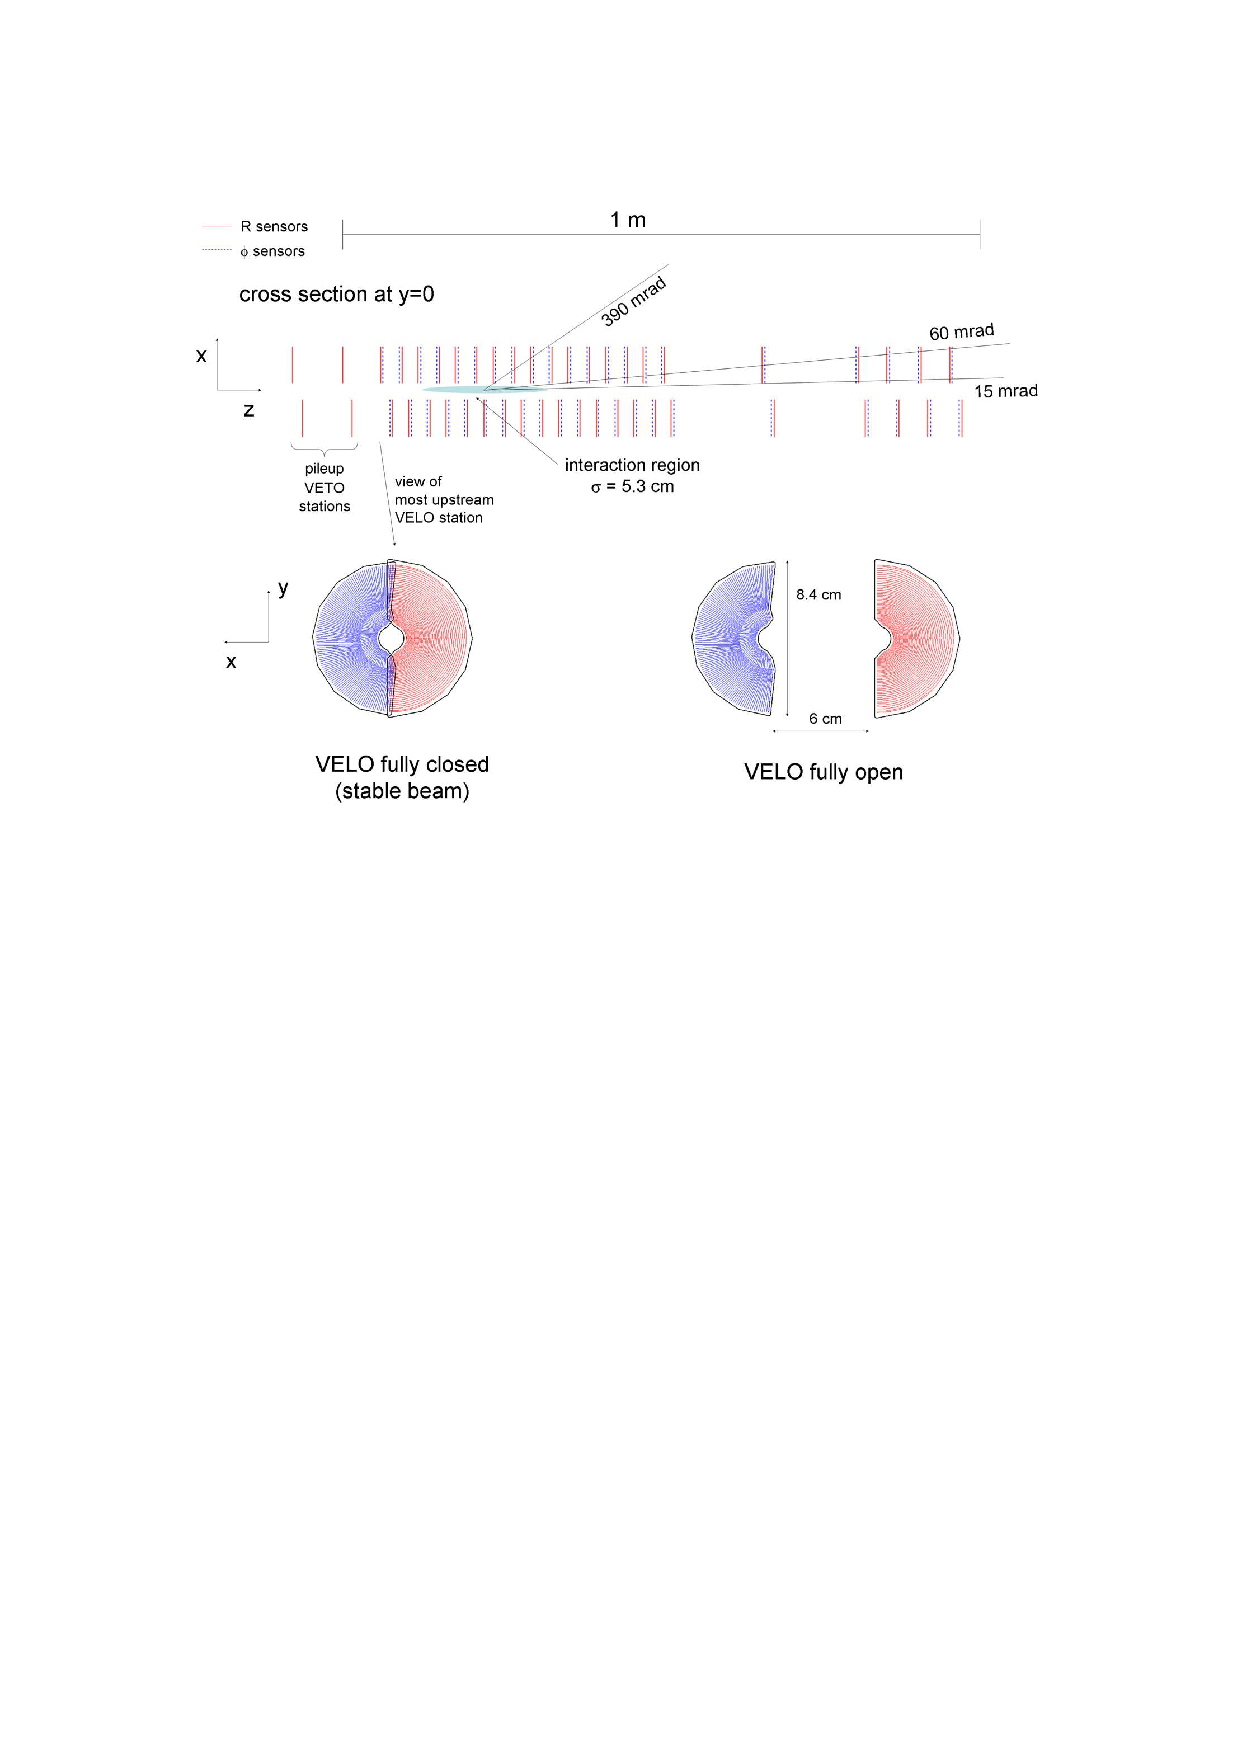
\includegraphics[width=0.7\textwidth]{fig/velo.pdf}
	\caption{Oben: Schnitt durch die $(x,z)$-Ebene des \velo bei $y=0$ bei geschlossenen Modulen. Unten: Sicht aus Strahlrichtung auf ein Modul im geschlossenen und geöffneten Zustand. Man erkennt die beiden Hälften zur $\phi$- (blau) und $r$-Messung (rot). \cite{Alves:2008zz}}
	\label{fig:velo} 
\end{figure} \\
Dabei wird zwischen einem inneren Teil nahe am Kollisionspunkt der Protonen und einem äußeren Teil strahlabwärts unterschieden. Bei einer Winkelakzeptanz von \SI{300}{mrad} bei \lhcb soll ein Teilchen mit diesem maximalen Winkel nun in mindestens drei Stationen Signale erzeugen, um rekonstruiert zu werden. Daraus folgt, dass der Abstand der inneren Stationen bei einem Radius der Sensoren von \SI{42}{mm} nicht größer als \SI{5}{cm} sein darf. Fordert man nun, unter der Annahme, dass einzelne Stationen nicht auslösen, dass in vier Stationen Signale erzeugt werden, kommt man auf einen Modulabstand von \SI{3{,}5}{cm} im inneren Teil des \velo. Außerdem wird durch diesen kleinen Abstand die mittlere Extrapolationsstrecke vom ersten gemessenen Treffer zum Vertex verkleinert.\\
Die untere Grenze der Winkelakzeptanz des \velo liegt bei \SI{15}{mrad} für Teilchen die, vom nominellen Interaktionspunkt der Protonen aus gesehen, bei $z=\SI{10{,}6}{cm}$ strahlabwärts entstehen.\\
Um die vollständige azimuthale Akzeptanz abzudecken, überlappen die beiden Detektorhälften jedes Moduls. Dies ist dadurch möglich, dass die $z$-Positionen der jeweiligen Hälften um \SI{1{,}5}{cm} zueinander verschoben sind (Abbildung \ref{fig:velo}).
 
\subsection{Die \rich-Detektoren}

Ein wichtiger Faktor bei \lhcb ist die Teilchenidentifikation, im Speziellen die Unterscheidung zwischen Pionen und Kaonen. Um diese gut zu realisieren, ist \lhcb mit zwei Ring-Imaging Cherenkov Detektoren, \richone und \richtwo, instrumentiert. Diese Detektoren nutzen den Cherenkov-Effekt, bei dem Teilchen sich in einem Medium mit einer höheren Geschwindigkeit bewegen als der Lichtgeschwindigkeit in diesem Medium. Diese Teilchen senden im Öffnungswinkel $\theta$ elektromagnetische Strahlung aus, wobei $\theta$ abhängig von der Geschwindigkeit der Teilchen ist:
\begin{equation}
\cos\left(\theta\right)=\frac{1}{n\beta}.
\end{equation}
Hier ist $n$ der Brechungsindex des durchflogenen Mediums und $\beta=$ \itshape\nicefrac{v}{c}\upshape. \\ 
Gemeinsam mit der Impulsinformation aus anderen Detektorkomponenten lässt sich dann gut zwischen verschiedenen Teilchen unterscheiden. Da sich das Impulsspektrum mit dem Polarwinkel (Winkel eines Teilchens zur Strahlachse) ändert, besteht das \rich-System aus den beiden Komponenten \richone und \richtwo. \richone identifiziert dabei Teilchen mit eher kleinen Impulsen von etwa \SI{1}{GeV\per c} bis \SI{60}{GeV\per c} \cite{Alves:2008zz} mit einer Mischung aus Aerogel und \cfourften, während \richtwo ein \cffour Gas verwendet und Teilchen mit größeren Impulsen im Bereich von $~$\SI{15}{GeV\per c} bis \SI{100}{GeV\per c} \cite{Alves:2008zz} unterscheidet. Wegen dieser unterschiedlicher Impulsbereichen ist \richone unmittelbar hinter dem \velo positioniert, während \richtwo erst hinter dem weiteren Tracking-System mit Magnet positioniert ist (Abbildung \ref{fig:det_plot}). 

\subsection{Das Tracking-System}


Das Tracking-System teilt sich in den Tracker Turicensis (\ttracker) und die drei Tracking-Stationen T$1$ bis T$3$ . Bei den Tracking-Stationen T$1$ bis T$3$ unterscheidet man weiter einen inneren Bereich nahe der Strahlröhre, den Inner Tracker (\intr), und entferntere Bereiche von der Strahlröhre, den Outer Tracker (\ot). Technologisch sind sowohl der \ttracker als auch der \intr Silizium Tracker (\st). Zum Tracking-System gehört außerdem ein Dipolmagnet mit einer integrierten Magnetfeldstärke von \SI{4}{Tm}, der zwischen dem \ttracker und dem restlichen Trackingsystem positioniert ist, sowie der in Abschnitt \ref{sec:velo} beschriebene \velo.\\
Die \st sind Detektoren aus Siliziumstreifen. Bei einer Breite der Siliziumstreifen von \SI{200}{\micro m} im \intr und \ttracker wird eine räumliche Auflösung von \SI{50}{\micro m} erreicht. Der \ttracker ist unmittelbar hinter dem \richone und vor dem Magneten installiert. Er ist \SI{150}{cm} breit und hat eine Höhe von \SI{130}{cm}. Der \intr ist in den drei Stationen  T$1$ bis T$3$ hinter dem Magneten im zentralen Bereich um das Strahlrohr installiert. Er deckt eine Fläche von \SI{120}{cm} Breite und \SI{40}{cm} Höhe ab (Abbildung \ref{fig:it}). 
\begin{figure}[htpb]
	\centering
		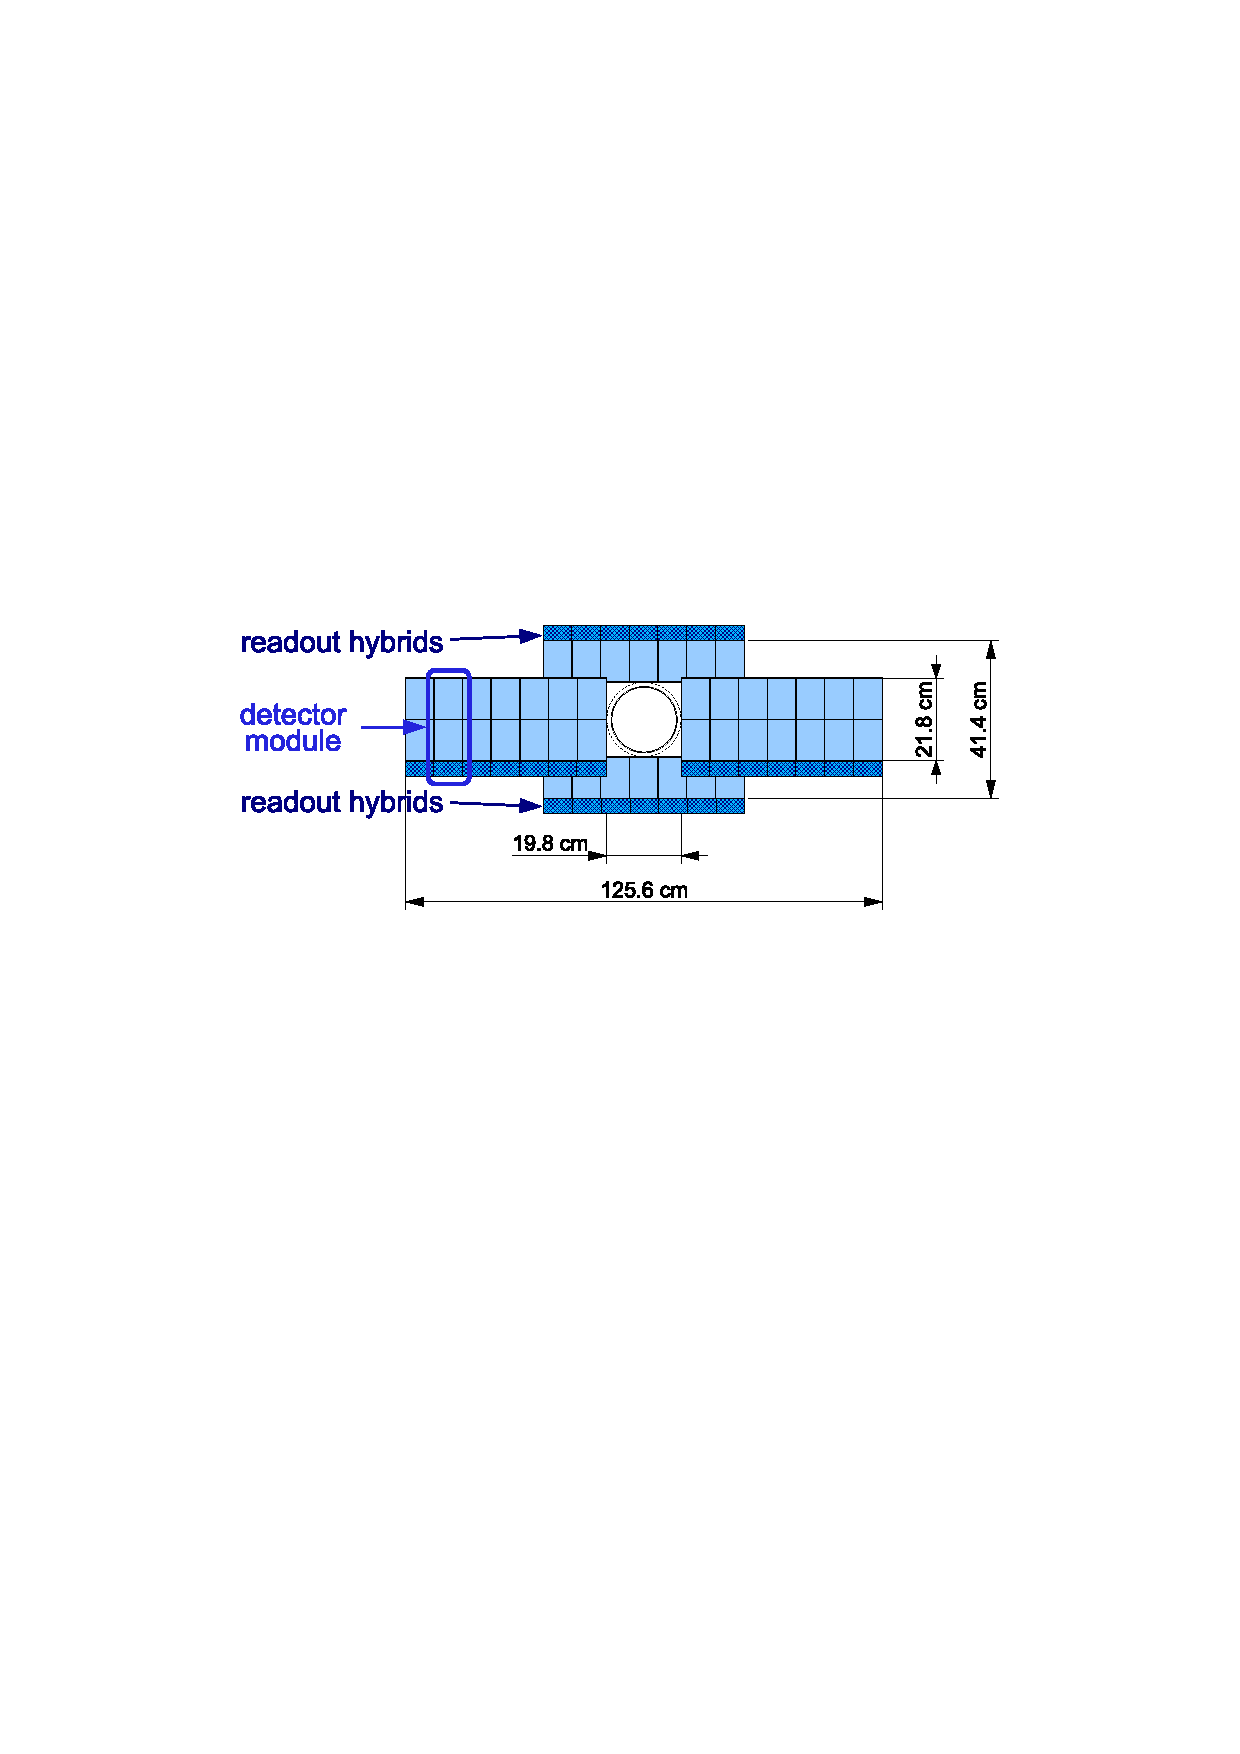
\includegraphics[width=0.7\textwidth]{fig/IT.pdf}
	\caption{Schematische Ansicht einer Schicht des \intr mit Auslesektronik. Eine Station setzt sich aus vier solcher Schichten zusammen, wobei die mittleren Schichten gegen die $(x,y)$-Ebene gekippt sind, um zusätzliche Winkelinformationen zu gewinnen. \cite{Alves:2008zz}}
	\label{fig:it} 
\end{figure}\\
Bei dem \ot handelt es sich um einen Detektor aus gasgefüllten Driftröhrchen. Dabei wird in den Driftröhrchen die Driftzeit ionisierter Gasatome und ihrer Elektronen gemessen und aus dieser Driftzeit auf die Ionisationsstelle geschlossen. Das Gasgemisch in den Driftröhrchen setzt sich dabei zu \SI{70}{\%} aus Argon, zu \SI{28{,}5}{\%} aus \cotwo  und zu \SI{1{,}5}{\%} aus {\ensuremath{\rm O_2}\xspace}  zusammen. Durch diese Zusammensetzung garantiert es möglichst schnelle Driftzeiten von unter \SI{50}{ns} und trotz allem eine hohe räumliche Auflösung von \SI{200}{\micro m}. Die Impulsauflösung des \ot beträgt $\frac{\delta p}{p}\approx\SI{0{,}4}{\%}$, bei einer Gesamtrekonstruktionseffizienz von \SI{80}{\%} \cite{Alves:2008zz}.\\
Alle Trackingstationen, das heißt sowohl der \ttracker als auch die Stationen T$1$ bis T$3$, sind aus jeweils vier Lagen aufgebaut, wobei die mittleren Lagen jeweils um $\pm$\SI{5}{\degree} um die Strahl-Achse gedreht sind, sodass sich die $y$-Koordinate eines Treffers, den ein Teilchen hinterlässt, bestimmen lässt. 

\subsection{Kalorimeter}

Die Kalorimeter haben verschiedene Aufgaben zu erfüllen. Zum einen unterstützen sie die \en-, \g- und Hadronenidentifizierungen, zum anderen messen sie Teilchenenergien und Positionen. Weiterhin selektieren sie Kandidaten für die erste Triggerstufe, den L$0$-Trigger, der bereits \SI{4}{\micro s} nach einer Wechselwirkung erste Entscheidungen trifft. Insgesamt folgt der Kalorimeteraufbau bei \lhcb der klassischen Abfolge. Auf ein elektromagnetisches Kalorimeter (\ecal) folgt ein hadronisches Kalorimeter (\hcal). Das \ecal ist dabei für die \en-Identifikationen verantwortlich.\\
Um  Untergründe von geladenen Pionen zu unterdrücken, ist vor dem \ecal der Preshower (\presh) installiert . Für die Trigger werden Untergründe von \piz mit hoher Transversalenergie $\et$ durch den Scintillating Pad Detector (\spd) unterdrückt.
Da die Trefferdichte über die Kalorimeterfläche um zwei Größenordnung variiert, ist die laterale Aufteilung der Kalorimeter je nach Abstand zur Strahlröhre unterschiedlich und wird mit der Entfernung zur Strahlröhre größer (Abbildung \ref{fig:kalos}).
\begin{figure}[htpb]
	\centering
		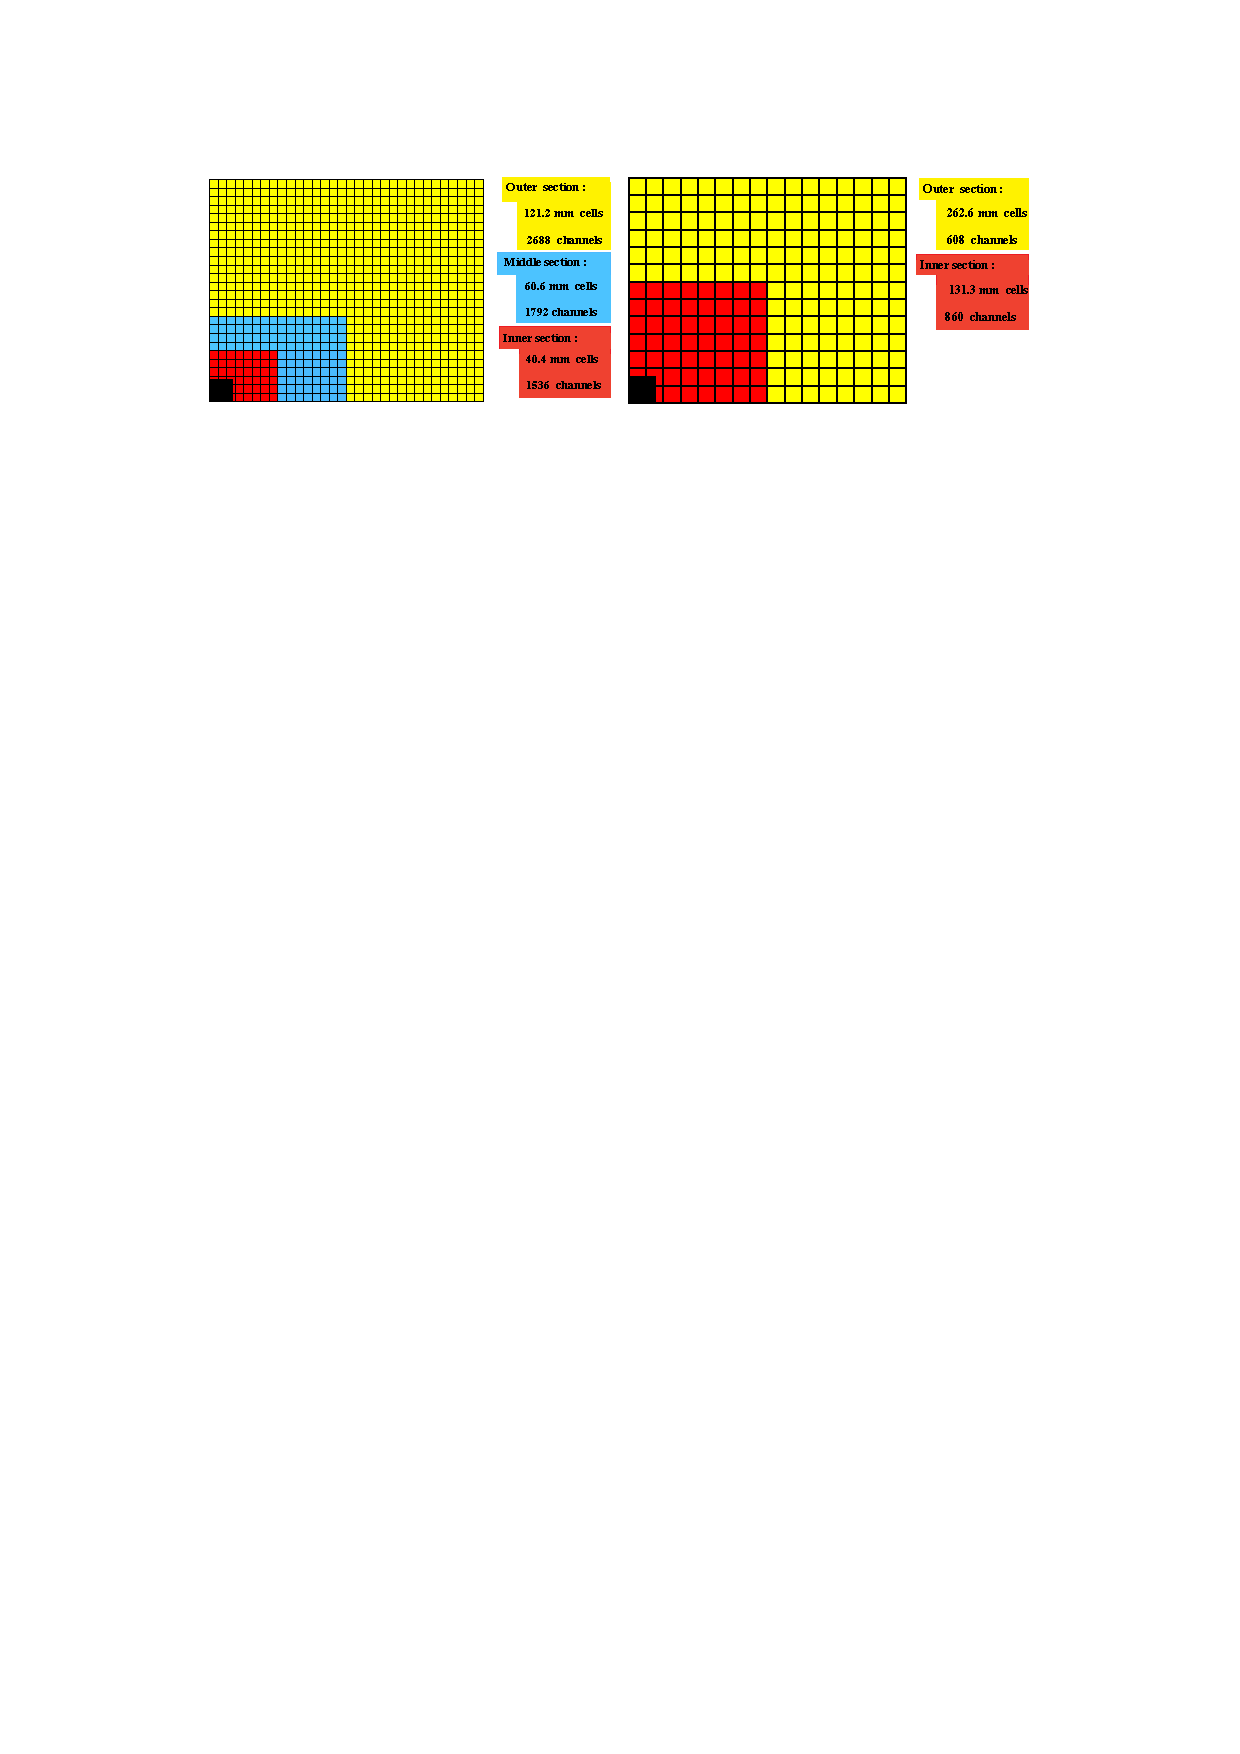
\includegraphics[width=0.9\textwidth]{fig/kalos.pdf}
	\caption{Laterale Aufteilung von \presh, \spd und \ecal (links) sowie vom \hcal (rechts). Zu sehen ist ein Viertel der Vorderansicht des Detektors. In schwarz ist der für das Strahlrohr ausgesparte Bereich dargestellt. \cite{Alves:2008zz}}
	\label{fig:kalos} 
\end{figure}

\subsection{Die Myonenkammern}

Die Detektion von Myonen ist von fundamentaler Wichtigkeit für \lhcb. Sowohl in vielen \CP-sensitiven Zerfällen, wie $\Bd\rightarrow\jpsi\KS$, in dem das \jpsi im Zerfall nach zwei Myonen rekonstruiert wird, als auch in seltenen $\B$-Zerfällen mit flavour-ändernden neutralen Strömen, wie $\Bs\rightarrow\mup\mun$, sind sie in Endzuständen zu finden. Bei \lhcb gibt es fünf Myonenkammern. Die Kammer M$1$ befindet sich vor den Kalorimetern, während M$2$ bis M$5$ hinter diesen positioniert sind. Die einzelnen Stationen sind dabei von \SI{80}{cm} dicken Eisenabsorbern durchzogen, sodass der Minimalimpuls eines Myons, um alle fünf Stationen zu passieren, \SI{6}{GeV} betragen muss. Die Stationen M$1$ bis M$3$ haben eine relativ hohe räumliche Auflösung entlang der $x$-Koordinate. Sie werden vor allem genutzt, um die Spurrichtungen zu identifizieren und den Transversalimpuls \pt der Myonkandidaten mit einer Auflösung von \SI{20}{\%} zu messen. Die Stationen M$4$ und M$5$ dienen dagegen eher der Teilchenidentifikation eindringender Myonen.  

\subsection{Trigger}\label{sec:trigger}

Das \lhcb-Experiment arbeitet nicht, wie die Vielzweckexperimente \atlas und \cms, bei der maximalen vom \lhc zur Verfügung gestellten Luminosität von $L\approx\SI[exponent-product = \cdot]{7e33}{cm^{-2}s^{-1}}$, sondern bei einer Luminosität von $L=\SI[exponent-product = \cdot]{4e32}{cm^{-2}s^{-1}}$, um im Idealfall pro Protonenpaketkollision exakt eine Proton-Proton-Wechselwirkung aufzunehmen. Trotzdem muss die Datenrate von etwa \SI{20}{MHz} noch auf etwa \SI{4}{kHz} reduziert werden, um gespeichert werden zu können. Dazu stehen zwei Trigger-Stufen zur Verfügung: Die erste Stufe (L$0$) arbeitet synchron zur Wechselwirkungsrate von \SI{40}{MHz} und reduziert diese auf \SI{1}{MHz}, woraufhin die zweite Trigger-Stufe, der High-Level-Trigger (HLT) unabhängig von der Wechselwirkungsrate die Daten weiterverarbeitet. Bei einer Luminosität von $L=\SI[exponent-product = \cdot]{4e32}{cm^{-2}s^{-1}}$ werden Ereignisse, die ein \B-Meson beinhalten, mit einer Rate von etwa \SI{15}{kHz} erzeugt. Weiterhin sind viele partielle Zerfallsbreiten der \B-Mesonen kleiner als $10^{-3}$, sodass das  Triggersystem dahingehend optimiert ist, diese interessanten Zerfälle für nachfolgende Analysen mit maximaler Effizienz zu selektieren, während die in der hadronischen Umgebung entstehenden Untergründe maximal unterdrückt werden \cite{Alves:2008zz}.\\
Bei dem Level-0-Trigger handelt es sich um einen reinen Hardware-Trigger. Er versucht zunächst die Hadronen, Elektronen und Photonen mit maximalen Transversalenergien \et, sowie die beiden Myonen mit den höchsten Transversalimpulsen \pt zu identifizieren. Dazu besteht der L$0$ aus drei Komponenten: Einem L$0$-pile-up-System, dem L$0$-Kalorimeter-Trigger und dem L$0$-Myon-Trigger. Ziel des pile-up-Systems ist dabei die Unterscheidung zwischen Events mit einer oder mehreren sichtbaren Proton-Proton-Wechselwirkungen. Die Kalorimeter- und Myon-Komponenten suchen für die entsprechenden Teilchen nach den maximalen \et beziehungsweise \pt.\\
Der HLT ist eine C++ Anwendung und läuft auf der sogenannten Event Filter Farm (EFF), einem Großrechner am \cern. Jede Anwendung hat dabei vollen Zugriff auf alle Informationen eines Events. Prinzipiell könnten hier also bereits Selektionsschritte durchgeführt werden. Da die Datenrate, die vom L$0$-Trigger kommt, jedoch sehr groß ist, besteht der HLT aus zwei Stufen. Der HLT$1$ rekonstruiert dabei die Teilchenkandidaten, die der L$0$ übergibt, im \velo und in den Tracking-Stationen. Außerdem werden hier für Photonen und neutrale Pionen die Abwesenheit geladener Teilchen bestätigt, die mit diesen beiden ungeladenen Kandidaten assoziiert werden könnten. Insgesamt hat der HLT$1$ die Aufgabe, die Datenrate so weit zu reduzieren, dass im nächsten Schritt, dem HLT$2$, eine vollständige Mustererkennung möglich ist. Bei einer ausreichend niedrigen Datenrate rekonstruiert der HLT$2$ dann schon teilweise spezifische \B-Zerfälle.

\subsection{\lhcb Software}

Die \lhcb-Software basiert auf dem \gaudi-Framework \cite{gaudi}, in dem verschiedene Software Pakete ausgeführt werden. Die Reihenfolge, in der die verschiedenen Pakete ausgeführt werden, ist in Abbildung \ref{fig:software} dargestellt.
\begin{figure}[htpb]
	\centering
		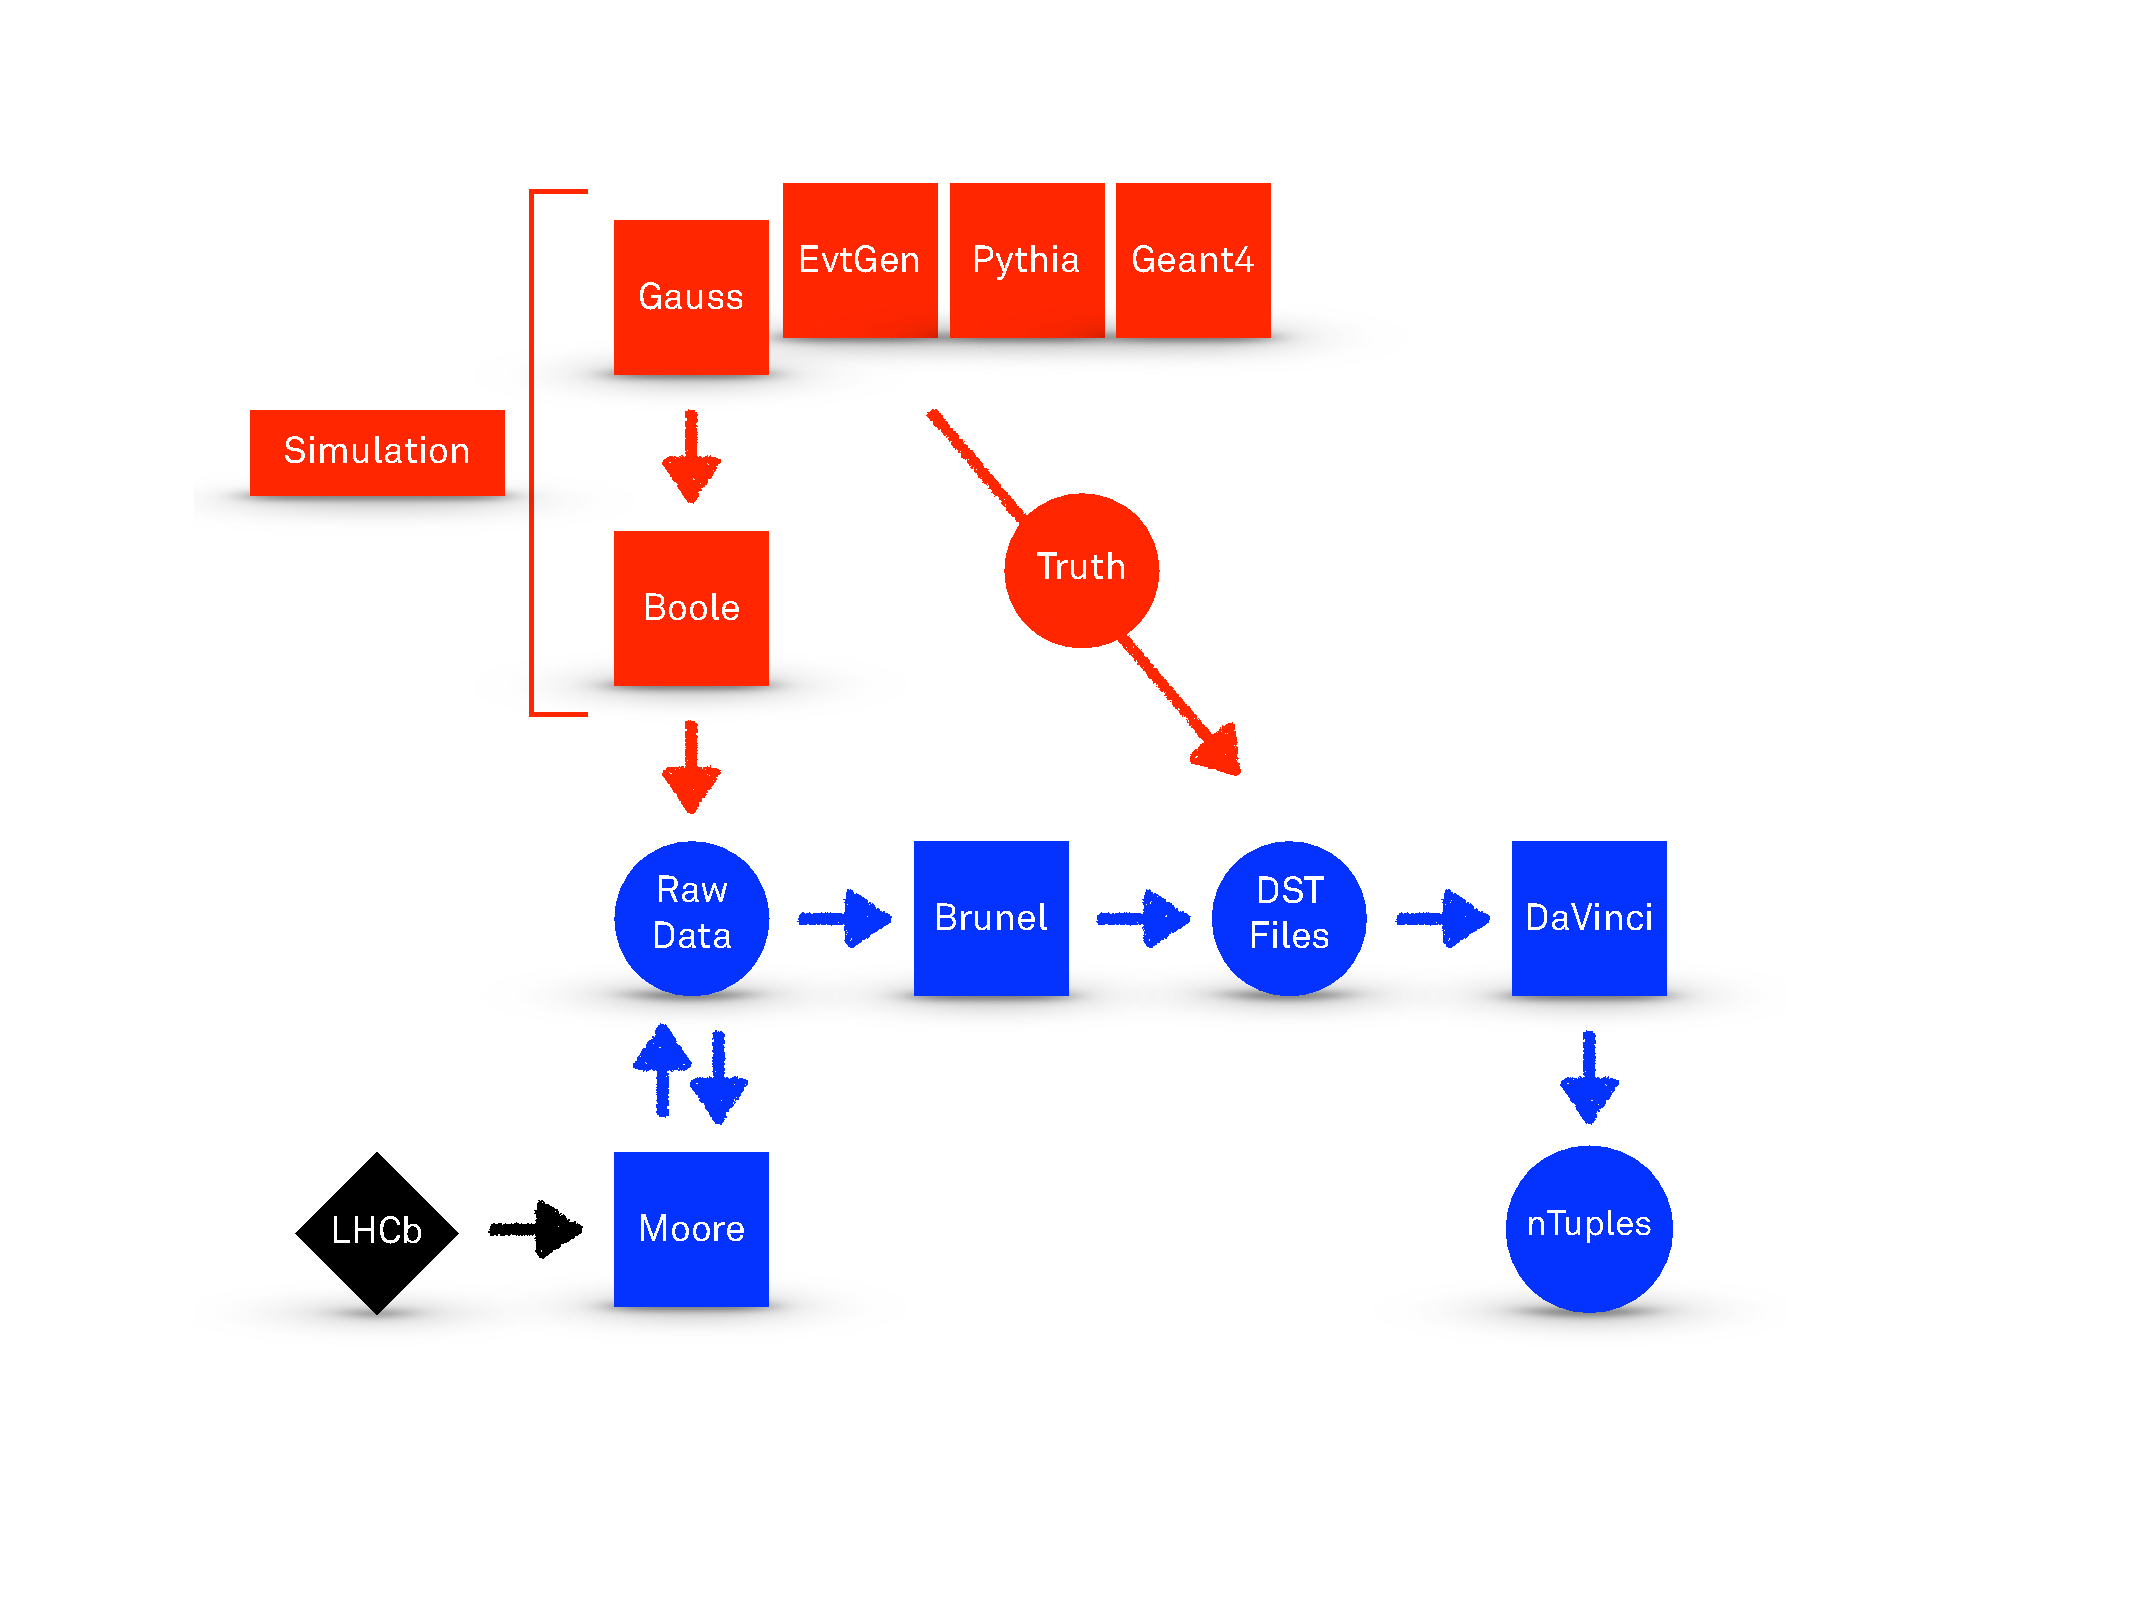
\includegraphics[width=0.7\textwidth]{fig/software.pdf}
	\caption{Abfolge der Datenprozessierung innerhalb der \lhcb-Software. In rot die Schritte zu Simulation von Daten, in blau die Prozessierung realer Daten. Die Software-Pakete sind dabei in Rechtecken, die übergebenen Datenformate in Kreisen dargestellt.}
	\label{fig:software} 
\end{figure}
Der erste Eingriff in die vom Detektor aufgenommen Daten passiert, wie in Abschnitt \ref{sec:trigger} beschrieben, beim HLT durch das Software Paket \moore \cite{moore}. Danach werden die Rohdaten in \brunel \cite{brunel} rekonstruiert und die Teilchen in sogenannten Protoparticles zusammengefasst. Diese Protoparticles haben dann sowohl Spurinformationen über das betreffende Teilchen, als auch Teilchenidentifikationsinformationen (PID-Informationen). Die nun als Data Summary Tape Dateien (DST's) vorliegenden Daten werden anschließen in \davinci \cite{davinci} weiter für die Analysen aufbereitet. Hier läuft sowohl eine erste Vorselektion, das sogenannte Stripping, in der die einzelnen Analysen speziell für ihre Bedürfnisse Schnitte auf physikalische Observablen definieren, als auch die finale Rekonstruktion der unterschiedlichen Prozesse. Ebenso wird an dieser Stelle das Flavour Tagging durchgeführt. Nachdem die Daten nun in Form von sogenannten nTuplen vorliegen, können diese mit \root \cite{root}, einer Sammlung von C++ Bibliotheken, die auf statistische Analysen der Hochenergiephysik spezialisiert sind, analysiert werden. Besonders hervorzuheben ist hier die \roofit \cite{roofit} Bibliothek, die bereits viele Parametrisierungen zur statistischen Modellierung der Daten beinhaltet. \\
Die Simulation von Daten wird bei \lhcb im \gauss Paket \cite{gauss} umgesetzt. Dieses ruft zunächst die Programmpakete \evtgen \cite{evtgen}, \pythia \cite{pythia6,pythia8}, das mit einer speziellen \lhcb Konfiguration \cite{lhcbconf} läuft, und \geant \cite{geant1,geant2} auf, die nacheinander die Proton-Proton-Kollisionen, den Hadronisationsprozess und die Wechselwirkung mit dem Detektor simulieren. Anschließend folgt \boole \cite{boole}, das die Daten digitalisiert, sodass diese anschließend wie die rohen Detektordaten verwendet werden können. Die Wahrheits- (Truth-)Informationen werden ebenfalls gespeichert und sind am Ende der Prozessierung bei der Analyse abrufbar. So sind in den Simulationen, neben den Detektorantworten, auch die anfangs generierten Zustände bekannt.  

  % !TEX root = main.tex
\chapter{Flavour Tagging am \lhcb Experiment}

Um die \CP-Verletzung in der Interferenz aus Mischung und Zerfall zu messen, muss der initiale Flavour des zerfallenden \B-Mesons bekannt sein, also ob es sich um ein \Bz- oder ein \Bzb-Meson handelt (Gleichung \eqref{eq:cpv}). Dies wird bei \lhcb durch das sogenannte Flavour Tagging festgestellt. Dabei geben verschiedene Algorithmen (Tagger) für jeden Kandidaten sowohl eine Entscheidung darüber, um welchen Flavour es sich gehandelt hat, als auch eine Wahrscheinlichkeit mit der Entscheidung falsch zu liegen, aus. Es wird dabei zwischen Taggern der Same Side (SS) und Taggern der Opposite Side (OS) unterschieden. Die SS Tagger untersuchen Teilchen, die in direktem Zusammenhang mit dem Hadronisierungsprozess entstehen, der beim Signal \bquark-Quark abläuft. Die OS Tagger analysieren den Hadronisierungsprozess des zweiten, mit dem Signal \bquark-Quark (\bquarkbar-Quark) gemeinsam erzeugten \bquarkbar-Quarks (\bquark-Quark) (Abbildung \ref{fig:flavourtagging}). Zum Abschluss wird schließlich die Selbsteinschätzung der Tagger zu einer \enquote{wahren} Wahrscheinlichkeit umgerechnet. 
\begin{figure}[htpb]
	\centering
		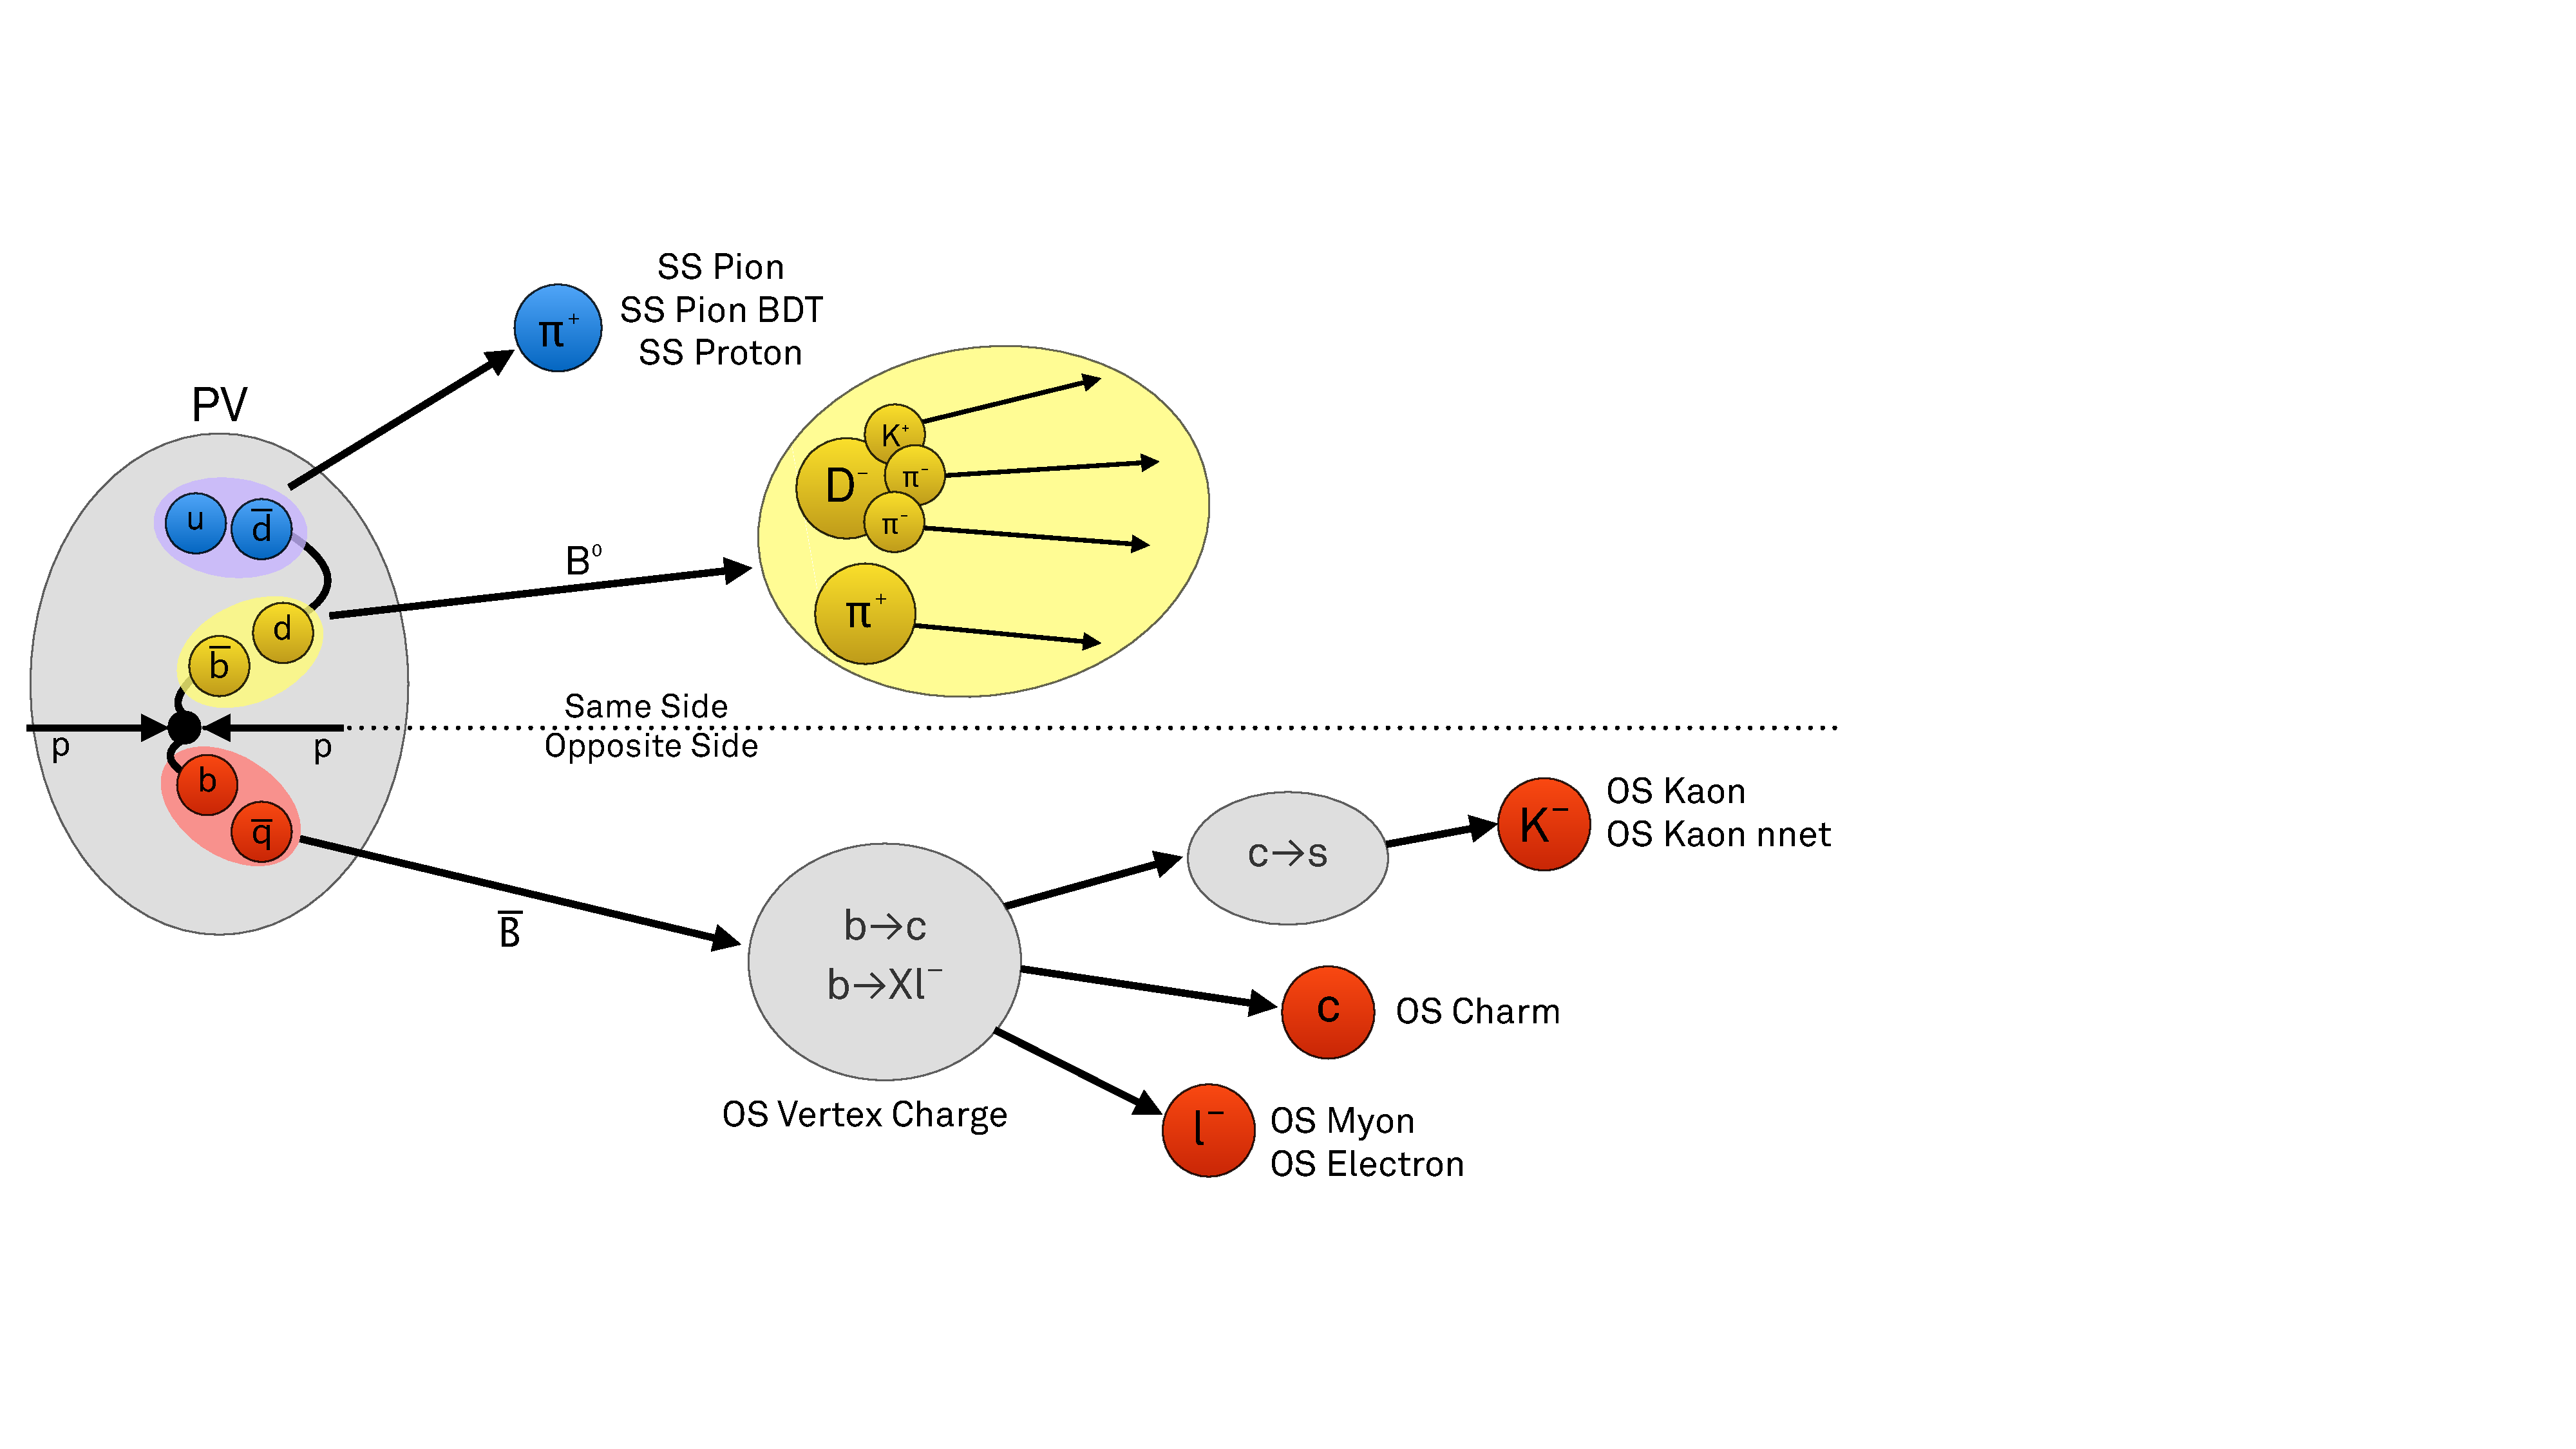
\includegraphics[width=\textwidth]{fig/FT_schema.pdf}
	\caption{Schematische Übersicht der Tagger, die in dieser Arbeit auf dem Kanal $\Bz\rightarrow D^-\pi^+$ kalibriert wurden.}
	\label{fig:flavourtagging} 
\end{figure}   

\section{Charakteristische Größen des Flavour Taggings}\label{sec:FTgrosse}

Jeder Tagger gibt zu jedem Kandidaten eine individuelle Entscheidung $d$ über den anfänglichen Flavour des \B-Mesons aus. Bei dieser Entscheidung, auch tag genannt, gibt es drei Möglichkeiten: als \Bz (\bquarkbar\dquark) getagged, als \Bzb (\bquark\dquarkbar) getagged oder ungetagged ($d=1$ entspricht einem \bquarkbar-Quark, $d=-1$ einem \bquark-Quark und $d=0$ einem ungetaggten Kandidaten). Außerdem erhält man zu jedem Kandidaten eine mistag-Wahrscheinlichkeit $\eta$, die eine Selbsteinschätzung der Wahrscheinlichkeit ist, mit der der Tagger bei einem Kandidaten falsch liegt. Da dies jedoch nur eine Abschätzung des Taggers über die Qualität seiner Entscheidung ist, wird die tatsächliche, kalibrierte Wahrscheinlichkeit mit der der Tagger falsch liegt mit 
\begin{equation}
\omega=\frac{N_{\text{R}}}{N_{\text{R}}+N_{\text{W}}}\label{eq:omega}
\end{equation}
dem true-mistag oder der true-mistag-Wahrscheinlichkeit bezeichnet. Dabei sind $N_{\text{R}}$ die Anzahl korrekt getaggter Ereignisse und $N_{\text{W}}$ die Anzahl falsch getaggter Ereignisse. Auf Monte-Carlo lässt sich nach Gleichung \eqref{eq:omega} aus den Truth-Informationen eine wahre mistag-Wahrscheinlichkeit berechnen, während auf Daten nur eine kalibrierte mistag-Wahrscheinlichkeit ermittelbar ist. Beachtet man diese Unsicherheit über den Anfangszustand nun für die gemessene Mischungsasymmetrie der \B-Mesonen (Gleichung \eqref{eq:mixing}) erhält man
\begin{equation}
\begin{split}
A_{\text{mix}}^{\text{tag}}&=\frac{\left(1-\omega\right)N_\text{unmixed}+\omega N_\text{mixed}-\left(1-\omega\right)N_\text{mixed}-\omega N_\text{unmixed}}{\left(1-\omega\right)N_\text{unmixed}+\omega N_\text{mixed}+\left(1-\omega\right)N_\text{mixed}+\omega N_\text{unmixed}}\\
&=\left(1-2\omega\right)\frac{N_\text{unmixed}-N_\text{mixed}}{N_\text{unmixed}+N_\text{mixed}}=\left(1-2\omega\right)\cos(\dm t).\label{eq:mischung}
\end{split}
\end{equation}
Analog dazu erhält man für eine gemessene \CP-Asymmetrie (Gleichung \eqref{eq:cpv})
\begin{equation}
A_\CP^{\text{tag}}=\left(1-2\omega\right)\frac{2\mathcal{Im}(\lambda_f)}{1+\left|\lambda_f\right|^2}\sin\left(\dm t\right).
\end{equation}
Man erkennt, dass durch die experimentelle Unsicherheit, die durch das Flavour Tagging hinzukommt, die Amplituden beider Asymmetrien um den gleichen Faktor abgeschwächt werden. Bei einem true-mistag von $\omega=0{,}5$ würden so beide Asymmetrien im Experiment verschwinden. Dieser Faktor wird Dilution $D$ genannt: 
\begin{equation}
D=1-2\omega
\end{equation}
Die einzelnen Tagger unterscheiden sich weiterhin in ihren Effizienzen. So ist die Anzahl der gettagten Ereignisse nicht für alle Tagger gleich, sodass  man die Taggingeffizienz
\begin{equation}
\varepsilon=\frac{N_{\text{R}}+N_{\text{W}}}{N_{\text{R}}+N_{\text{W}}+N_{\text{U}}}
\end{equation}
definiert, bei der neben Kandidaten mit einem Tag ($N_\text{R}$ und $N_\text{W}$) auch ungetaggte Kandidaten ($N_\text{U}$) berücksichtigt werden. Weiterhin wird die effektive Taggingeffizienz
\begin{equation}
\varepsilon_\text{eff}=\varepsilon D^2
\end{equation}
eingeführt. Über diese lassen sich einzelne Tagger nun untereinander in ihrer Leistung vergleichen. So ist die effektive Taggingeffizienz $\varepsilon_\text{eff}$ auch ein Maß für die statistische Größe des zu untersuchenden Datensatzes. Multipliziert man die Anzahl Ereignisse eines Datensatzes mit dieser effektiven Taggingeffizienz $\varepsilon_\text{eff}$, so erhält man die Anzahl Kandidaten, die man bei einem perfekt getaggten Datensatz für die gleiche statistische Aussagekraft auf die Messung einer physikalischen Observablen wie \dmd oder $\sin\left(2\beta\right)$ benötigen würde. Dabei bedeutet perfekt getaggter Datensatz, das für jeden Kandidaten eine korrekte Tag-Entscheidung mit einem mistag von $\omega=0$ getroffen wurde.\\
Die bisher eingeführten Größen, speziell der true-mistag, beachtet keine Asymmetrie im Tagging zwischen \Bz- und \Bzb-Mesonen. Zieht man diese hinzu, lässt sich ein true-mistag $\omega$ für getaggte \Bz-Mesonen und $\overline{\omega}$ für getaggte \Bzb-Mesonen definieren. Der bisher verwendete true-mistag ist dann als mittlerer true-mistag 
\begin{equation}
\widetilde{\omega}=\frac{\omega+\overline{\omega}}{2}
\end{equation}
zu betrachten. Somit lässt sich eine mistag-Asymmetrie $\Delta\omega=\omega-\overline{\omega}$ definieren.

\section{Opposite Side Tagging}\label{sec:ostagging}

Beim Opposite Side Tagging wird der Hadronisierungsprozess des \bquark-Quarks ausgenutzt, welches nicht das \B-Meson des Signalzerfalls bildet. Dazu werden zum Einen einzelne Teilchen wie Elektronen, Myonen, Kaonen oder \D-Mesonen identifiziert, die im Zusammenhang mit Hadronisierungs- und Zerfallsprozessen dieses sogenannten Opposite Side \bquark-Quarks entstehen, zum Anderen nutzt einer der Tagger die Ladung von Spuren, die aus einem gemeinsamen Sekundärvertex kommen, der nicht mit dem Signal \B assoziiert ist (Abbildung \ref{fig:flavourtagging}). Da das Opposite Side \B-Meson unabhängig vom Signal \B-Meson sein sollte, also unabhängig von dessen Hadronisierungsprozess, können die Tagger sowohl für {{\ensuremath{\B^0_\dquark}}\xspace}-, als auch für  \Bs-Mesonen gleich verwendet werden. Im Folgenden soll nun in Anlehnung an \cite{tagging} auf die einzelnen Tagger eingegangen werden.
\begin{itemize}
\item Der OS Myon Tagger nutzt Myonen aus semileptonischen \B-Zerfällen um eine Tagentscheidung zu fällen. Davon ausgehend, dass das Opposite Side \B-Meson nicht gemischt hat, lässt sich aus der Ladung des Myons auf den anfänglichen Flavour des \B-Mesons schließen. Um tatsächlich Myonen der Opposite Side zu rekonstruieren, werden unterschiedliche Schnitte angewendet. Beiträge aus $\bquark\rightarrow\cquark\rightarrow\lepton$, was die falsche Ladung und damit den falschen Tag zur Folge hätte, werden beispielsweise durch einen Schnitt auf den Transversalimpuls $\pt>\SI{1{,}2}{GeV\per c}$ unterdrückt. Wenn nach den verschiedenen Selektionsschritten noch mehrere Myonenkandidaten übrig bleiben, wird das Myon mit dem höchsten Transversalimpuls $\pt$ für die Tagentscheidung genutzt.
\item Der OS Elektron Tagger funktioniert analog zum OS Myon Tagger. Auch hier gibt die Ladung eines Elektrons aus einem semileptonischen Zerfall des Opposite Side \B-Mesons Aufschluss über den anfänglichen Flavour des \B-Mesons. Die Elektronenselektion funktioniert ebenfalls durch einfache rechtwinklige Schnitte, wobei zusätzlich hilfreiche Variablen für die Elektronenidentifikation genutzt werden. Zu diesen gehört das Verhältnis der Teilchenenergie $E$, gemessen im \ecal und des Impulses $p$ des Elektronkandidaten. Dabei wird $E/p>0{,}8$ gefordert. Ebenfalls analog zum Myon-Tagger wird bei mehreren Elektronenkandidaten der Kandidat mit dem höchsten Transversalimpuls \pt für die Tagentscheidung gewählt
\item Der OS Kaon Tagger nutzt Kaonen aus der Zerfallskette $\bquark\rightarrow\cquark\rightarrow\squark$. Aus der Ladung des Kaons lässt sich wiederum auf den Flavour des \B-Mesons schließen, nimmt man an, dass das Opposite Side \B-Meson nicht gemischt hat. Bei dem schnittbasierten OS Kaon Tagger werden ebenfalls rechtwinklige Schnitte angewendet, um den Kaonkandidaten zu selektieren. Abschließend wird bei mehreren Kaonkandidaten wieder der Kandidat mit dem höchsten Transversalimpuls \pt gewählt. Beim Tagging mit OS-Kaonen gibt es zusätzlich eine Neuentwicklung, den OS Kaon nnet. Dieser selektiert die Kaonen nicht über rechtwinklige Schnitte, sondern nutzt ein neuronales Netz. So erhält man zwar deutlich mehr getaggte Ereignisse, die mistag's sind jedoch im Mittel größer.
\item Der OS Vertex Charge Tagger ist der einzige Tagger, der keine Einzelteilchen rekonstruiert, sondern die gesamte gewichtete Ladung eines zum Opposite Side \B-Mesons assoziierten Sekundärvertex (SV) für seine Tagentscheidung nutzt. Dabei wird zunächst aus zwei Spuren ein Sekundärvertex rekonstruiert, wobei aus allen Spuren das Spurenpaar gewählt wird, das die höchste Wahrscheinlichkeit besitzt aus dem Opposite Side \B-Meson zu stammen. Anschließend werden nach einigen geometrischen und kinematischen Schnitten weitere Spuren zu dem gebildeten SV hinzugefügt. Aus diesen Spuren wird anschließend die gewichtete Ladung des SV
\begin{equation}
Q_\text{Vtx}=\frac{\sum_{i}\pt^k(i)Q_i}{\sum_{i}\pt^k(i)}
\end{equation}
gebildet. Der Parameter $k$ ist dabei dahingehend optimiert, eine maximale effektive Taggingeffizienz $\varepsilon_\text{eff}$ zu liefern.
\item Bei dem OS Charm Tagger handelt es sich ebenfalls um eine Neuentwicklung. Er trifft seine Entscheidungen basierend auf rekonstruierten \D-Mesonen, die vor allem aus der Zerfallskette $\bquark\rightarrow\cquark$ entstammen. Dabei gibt im Falle eines geladenen \D-Mesons dessen Ladung direkt Aufschluss über den anfänglichen Flavour des \B-Mesons, bei einem ungeladenen \D-Meson die Ladung des Kaons, in das das \D-Meson zerfällt. Die \D-Kandidaten werden dabei über einen Boosted Decision Tree (BDT) rekonstruiert. Der OS Charm Tagger wurde dabei, bei einem geringen Überlapp mit den anderen Taggern, auf eine maximale effektive Taggingeffizienz $\varepsilon D^2$ optimiert, sodass er im Vergleich zu den anderen Taggern relativ kleine Taggingeffizienzen $\varepsilon$ bei allerdings auch guten mistag-Vorhersagen liefert.
\end{itemize}
Die einzelnen Tagger können kombiniert werden, um die unterschiedlichen Vorhersagen zu nutzen und die effektive Taggingeffizienz $\varepsilon D^2$ des Datensatzes zu erhöhen. Dabei wird die kombinierte Wahrscheinlichkeit, dass das \B-Meson ein \bquark-Quark enthält, berechnet als
\begin{equation}
P(\bquark)=\frac{p(\bquark)}{p(\bquark)+p(\bquarkbar)} \hspace{1cm}\text{und}\hspace{1cm}P(\bquarkbar)=1-P(\bquark)
\end{equation}
wobei die Wahrscheinlichkeiten $p(\bquark)$ und $p(\bquarkbar)$ als
\begin{equation}
p(\bquark)=\prod_{i}\left(\frac{1+d_i}{2}-d_i\left(1-\eta_i\right)\right)
\end{equation}
und
\begin{equation}
p(\bquarkbar)=\prod_{i}\left(\frac{1-d_i}{2}+d_i\left(1-\eta_i\right)\right)
\end{equation}
definiert sind. Dabei sind $d_i$ die Entscheidungen und $\eta_i$ die mistag Vorhersagen der einzelnen Tagger. Die kombinierte Entscheidung und mistag Vorhersage ergibt sich für $P(\bquark)>P(\bquarkbar)$ nun zu $d=-1$ und $\eta=1-P(\bquark)$ und für $P(\bquark)<P(\bquarkbar)$ zu $d=1$ und $\eta=P(\bquark)$.\\
In der Flavour Tagging Software ist eine Kombination der OS Tagger direkt implementiert. Diese Standard OS Kombination enthält aktuell den OS Myon, den OS Elektron, den OS Kaon und den OS Vertex Charge Tagger, da es sich bei diesen um die bereits etablierten Tagger handelt.

\section{Same Side Tagging}

Beim Same Side Tagging werden direkt Abhängigkeiten bei der Hadronisierung des Signal \B-Mesons ausgenutzt. Im Falle eines \Bz (\bquarkbar\dquark) bleibt beispielsweise ein freies \dquarkbar-Quark, das zu einem Pion oder Proton hadronisieren kann. Im Falle eines \Bs (\bquarkbar\squark) bleibt ein freies \squarkbar-Quark, das zu einem Kaon hadronisieren kann. Für Pionen und Kaonen sind zwei beispielhafte Hadronisierungsprozesse in Abbildung \ref{fig:FThadronisierung} dargestellt.
\begin{figure}[htpb]
	\centering
		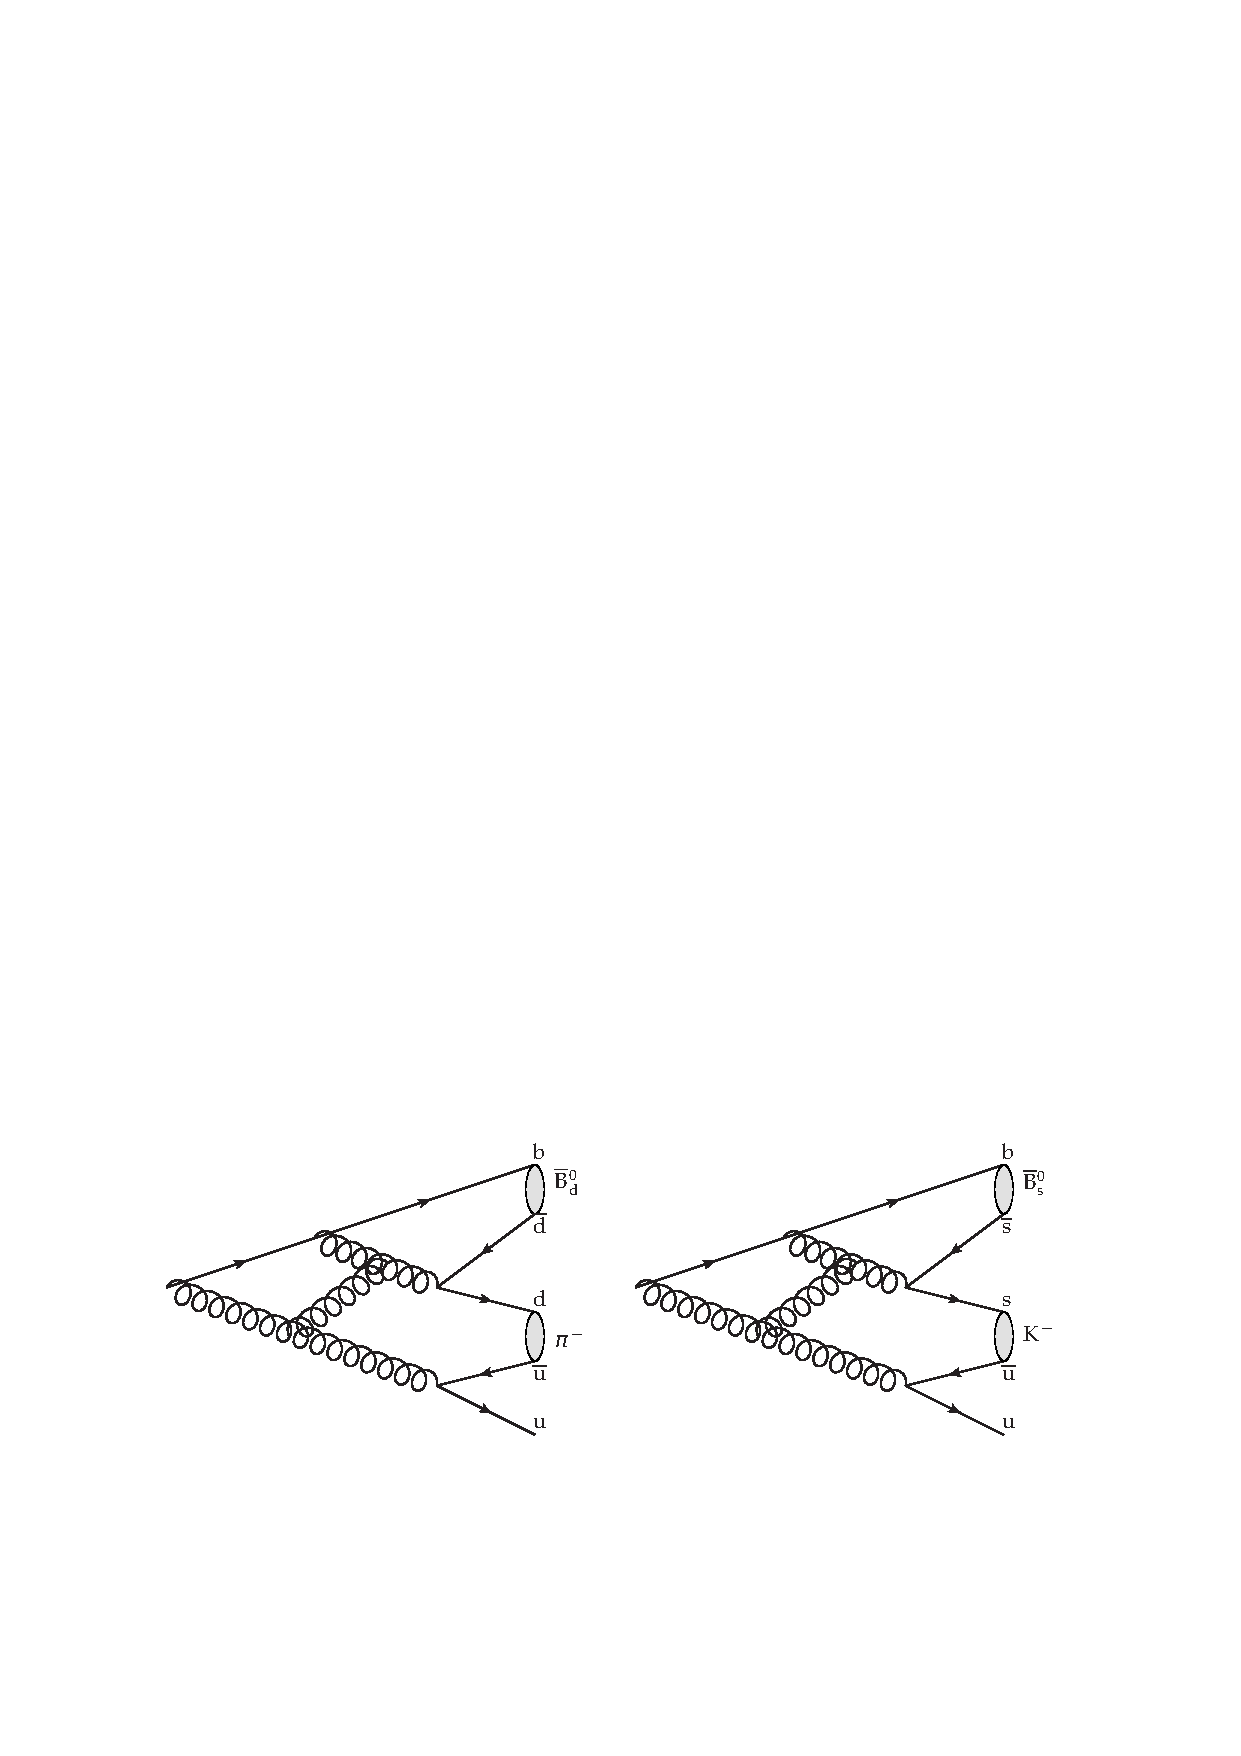
\includegraphics[width=0.8\textwidth]{fig/FThadronisierung.pdf}
	\caption{Feynmandiagramme der \Bz und \Bs Hadronisation. \cite{tagging}}
	\label{fig:FThadronisierung} 
\end{figure} 
Die einzelnen Tagger sollen nun im Folgenden wiederum in Anlehnung an \cite{tagging} genauer vorgestellt werden.
\begin{itemize}
\item Der SS Pion Tagger nutzt in \Bz-Zerfällen die Ladung eines im Hadronisationsprozess entstehenden Pions. Dabei werden sowohl Pionen, die direkt aus einem zusätzlichen \dquark-Quark (Abbildung \ref{fig:FThadronisierung} links) beim \Bz stammen genutzt, als auch Pionen aus höher angeregten \B-Zuständen, wie dem {{\ensuremath{\B^{0*}}}\xspace} oder dem {{\ensuremath{\B^{0**}}}\xspace}. Die Selektion des SS Pion Taggers basiert, ebenso wie bei den meisten OS Taggern, auf rechtwinkligen Schnitten. Dabei werden ähnliche Kriterien wie bei der Auswahl für die OS Tagger angewendet, um geeignete Pionen zu rekonstruieren, wie Schnitte auf den Transversalimpuls der Kandidaten. Ebenso wird, falls mehrere Pion Kandidaten vorliegen, analog der Kandidat mit dem höchsten Transversalimpuls \pt  für die Tagentscheidung gewählt. Ähnlich wie bei dem OS Kaon Tagger gibt es auch bei dem SS Pion Tagger eine Neuentwicklung, die auf einer multivariaten Methode basiert. Der SS Pion BDT Tagger nutzt zur Selektion  eines geeigneten Pion Kandidaten einen BDT. Auch hier erhält man mit der multivariaten Methode deutlich mehr getaggte \B-Mesonen, allerdings im Schnitt auch schlechtere mistag-Vorhersagen.
\item Der SS Proton Tagger ist ebenso wie der SS Pion BDT eine Neuentwicklung. Er funktioniert, wie die beiden SS Pion Tagger, für \Bz-Mesonen Zerfälle. Die Teilchenselektion basiert auf einem BDT und hat hohe Anzahlen an getaggten Ereignissen ($\varepsilon>\SI{30}{\%}$) und im Schnitt eher hohe mistag-Vorhersagen ($\langle\eta\rangle>0{,}4$).
\item Der SS Kaon Tagger ist für \Bs-Meson-Zerfälle entwickelt worden und arbeitet für diese analog zum SS Pion Tagger für \Bz-Ereignisse. Da in dieser Arbeit das Flavour Tagging im Kanal $\Bz\rightarrow\Dm\pip$ untersucht werden soll, wird auf den SS Kaon Tagger an dieser Stelle nicht weiter eingegangen.
\end{itemize}
Neben der möglichen Verwendung des SS Pion, des SS Pion BDT und des SS Proton Tagger für \Bz-Ereignisse lassen sich alle drei natürlich auch für \Bu-Ereignisse (\bquarkbar\uquark) nutzen um das Flavour Tagging zu kalibrieren. 

\section{Vorgehen bei der Tagging Kalibrierung}

Wie in Abschnitt \ref{sec:FTgrosse} bereits erwähnt, liefert jeder Tagger für jedes Ereignis eine Abschätzung $\eta$ der mistag Wahrscheinlichkeit. Diese Abschätzung muss für die Analyse von \CP-Asymmetrien auf die wahren mistags $\omega$ kalibriert werden. Dabei geht man von einem linearen Zusammenhang der Form
\begin{equation}
\widetilde{\omega}(\eta)=p_0+p_1\cdot\left(\eta-\langle\eta\rangle\right)\label{eq:linear}
\end{equation}
aus. Dabei ist $\langle\eta\rangle$ der Mittelwert aller $\eta$-Werte eines Taggers. Durch Subtrahieren dieses Wertes von den einzelnen $\eta$-Werten werden die Parameter $p_0$ und $p_1$ dekorreliert. Bei einem perfekt kalibrierten Tagger gilt, dass $p_0=\langle\eta\rangle$ und $p_1=1$ entspricht. Analog dazu lässt sich die mistag-Asymmetrie parametrisieren:
\begin{equation}
\Delta\omega(\eta)=\Delta p_0+\Delta p_1\cdot\left(\eta-\langle\eta\rangle\right)\label{eq:lineardelta}
\end{equation}
Die verschiedenen Tagger werden nun auf unterschiedlichen Zerfallskanälen kalibriert, sodass ein Satz aus Werten für die Parameter für $p_0$, $p_1$, $\Delta p_0$ und $\Delta p_1$ inklusive statistischer und systematischer Unsicherheiten entsteht. Für die globale Kalibrierung wird dann ein bestimmter Kanal verwendet, und die Abweichungen in den weiteren geprüften Kanälen werden genutzt um systematische Unsicherheiten zu ermitteln. Der Kanal \BdToDpi wurde zuletzt nicht verwendet, soll nun aber wieder in die Kombination der Flavour Tagging Gruppe eingehen.\\
Die möglichen Verfahren zur Tagging Kalibrierung unterscheiden sich für die Zerfälle von ungeladenen \B-Mesonen auf Monte-Carlo und Daten grundsätzlich und werden in den nächsten beiden Abschnitten erläutert.   

\subsection{Daten}\label{sec:kalibrierungDaten}

Da auf Daten der wahre Flavour für ungeladene \B-Mesonen nicht bekannt ist, lässt sich dieser nicht nach Gleichung \eqref{eq:omega} durch einfaches Abzählen bestimmen. Allerdings bietet die Mischungsasymmetrie (Gleichung \eqref{eq:mischung}) eine Möglichkeit $\omega$ zu bestimmen.\\ 
Im Folgenden wird dazu der Datensatz in Kategorien der mistag-Vorhersage $\eta$ eines Taggers geteilt. Dann werden Masse und Zerfallszeit simultan in diesen Kategorien der mistag-Vorhersage $\eta$ gefittet. Der Massenfit geschieht dabei, um besser zwischen den Signal und Untergrund-Komponenten zu unterscheiden. Bei der Parametrisierung der Zeit sind die Gleichungen \eqref{eq:uebergang1}, \eqref{eq:uebergang2}, \eqref{eq:uebergang3} und \eqref{eq:uebergang4} an die Unsicherheiten des Flavour Taggings anzupassen. Dabei wird hier weiter der Spezialfall der \Bz-Mesonen mit $\Gamma_H\approx\Gamma_L$ und $\left|\tfrac{q}{p}\right|=1$ betrachtet:
\begin{equation}
\begin{split}
\Gamma^\text{exp}\left(\Bzb\to f\right)&=\left(1-\overline{\omega}\right)\Gamma\left(\Bzb\to f\right)+\omega\cdot\Gamma\left(\Bz\to f\right)\\
\Gamma^\text{exp}\left(\Bz\to f\right)&=\left(1-\omega\right)\Gamma\left(\Bz\to f\right)+\overline{\omega}\cdot\Gamma\left(\Bzb\to f\right)\\
\Gamma^\text{exp}\left(\Bzb\to\overline{f}\right)&=\left(1-\overline{\omega}\right)\Gamma\left(\Bzb\to\overline{f}\right)+\omega\cdot\Gamma\left(\Bz\to\overline{f}\right)\\
\Gamma^\text{exp}\left(\Bz\to\overline{f}\right)&=\left(1-\omega\right)\Gamma\left(\Bz\to\overline{f}\right)+\overline{\omega}\cdot\Gamma\left(\Bzb\to\overline{f}\right).
\end{split}
\end{equation}
Mithilfe der Tagentscheidung $d$ und dem Mischungszustand $\xi$, der zwischen gemischten und ungemischten \B-Mesonen unterscheidet, lassen sich die vier unterschiedlichen Fälle zu
\begin{equation}
\Gamma^\text{exp}\left(\hat{B}\to\hat{f}\right)=\frac{1}{2}e^{-\Gamma t}\left[\left(1-d\Delta\omega\right)+\xi\left(1-2\widetilde{\omega}\right)\cos\left(\dmd t\right)\right]
\end{equation}
zusammenfassen, wobei mögliche asymmetrische mistag-Wahrscheinlichkeiten $\omega$ und $\overline{\omega}$ mit einem mittleren true-mistag $\widetilde{\omega}$ und der mistag-Asymmetrie $\Delta\omega$ beschrieben werden. Mit einer Unterscheidung zwischen den vor dem Zerfall gemischten und ungemischten Zuständen ist der Fit hier also sensitiv auf den mistag $\widetilde{\omega}$ in jeder Kategorie. Nach der Bestimmung von mittleren mistag-Vorhersagen $\eta$ in jeder Kategorie lassen sich so erhaltene $(\eta,\widetilde{\omega})$-Paare nun mit ein linearer Zusammenhang nach Gleichung \eqref{eq:linear} beschreiben. Da der Fit mit der tag-Entscheidung $d$ ebenso auf die mistag-Asymmetrie $\Delta \omega$ sensitiv ist, lässt sich diese analog gegen die Kategoriemittelwerte der mistag-Vorhersage $\eta$ auftragen und nach Gleichung \eqref{eq:lineardelta} kalibrieren.\\
Neben dieser in der Flavour Tagging Arbeitsgruppe zumeist durchgeführten Methode Tagger zu kalibrieren, soll außerdem ein weiteres Verfahren vorgestellt werden. Dabei werden die mistags $\eta$ in Wahrscheinlichkeiten $P_\text{tag}(\bquarkbar)$, dass das betroffene Teilchen ein \bquarkbar-Quark enthält, umgerechnet. Bei einer Tagentscheidung $d=-1$ ergibt sich also $P_\text{tag}(\bquarkbar)=\eta$ und bei einer Tagentscheidung $d=1$ erhält man $P_\text{tag}(\bquarkbar)=1-\eta$. Für ungetaggte Teilchen ist $P_\text{tag}(\bquarkbar)=0{,}5$. Nun wird der Datensatz in Kategorien dieser Wahrscheinlichkeit $P_\text{tag}(\bquarkbar)$ eingeteilt und der Zusammenhang zur wahre Wahrscheinlichkeit $P_\text{true}(\bquarkbar)$ kalibriert. Nun lassen sich die Bereiche für \bquarkbar ($0{,}5<P_\text{tag}(\bquarkbar)<1$) und für \bquark ($0<P_\text{tag}(\bquarkbar)<0{,}5$) einzeln mit linearen Funktionen der Form
\begin{equation}
P_\text{true}(P_\text{tag})=p_0+p_1\cdot\left(P_\text{tag}-\langle P_\text{tag}\rangle\right)\label{eq:linearPB},
\end{equation}
kalibrieren, wobei die Parameter in diesem Kontext für \Bz-Mesonen (\bquarkbar\dquark) im Weiteren mit $p_0$ und $p_1$ und für \Bzb-Mesonen (\bquark\dquarkbar) mit $\overline{p_0}$ und $\overline{p_1}$ bezeichnet werden sollen. Die Zentralwert für \Bz- und \Bzb-Mesonen werden dann mit $\widetilde{p_0}$ und $\widetilde{p_1}$ beschrieben.\\
Hintergrund dieser Methodik ist, dass die verschiedenen Tagger intern mit der Wahrscheinlichkeit $P(\bquarkbar)$ rechnen.

\subsection{Monte-Carlo}\label{sec:mckalibrierung}

Auf Monte-Carlo ist der generierte (wahre) Produktionsflavour der \B-Mesonen bekannt. So lässt sich durch Vergleich zwischen dem bekannten initialen Flavour eines Ereignisses und der entsprechenden Entscheidung eines Taggers erkennen, ob der Tagger mit seiner Entscheidung richtig oder falsch lag. Unterteilt man den Datensatz nun in Bins der mistag-Vorhersage $\eta$ des Taggers, kann man in jedem Bin den mittleren wahren mistag $\omega$ nach Gleichung \eqref{eq:omega} berechnen. Durch Berechnen der Mittelwerte der $\eta_i$ in jedem Bin lassen sich die zugehörigen mittleren mistag-Vorhersagen der Tagger berechnen. Trägt man nun die $\omega$ in Abhängigkeit von $\eta$ auf lässt sich der lineare Zusammenhang aus Gleichung \eqref{eq:linear} bestimmen. Dabei sind die $\eta$-Werte nun die Mittelwerte der $\eta_i$ und $\omega$ die wahren mistags in den einzelnen Bins.\\
Neben dieser einfachen Methode ließe sich auf Monte-Carlo auch ein simultaner Fit umsetzen um eine Kalibrierung durchzuführen. Da auf Monte-Carlo jedoch der Untergrund explizit ausgeschaltet werden kann, wird hier neben dem Lebenszeitfit zur Bestimmung der mistag-Wahrscheinlichkeiten $\widetilde{\omega}$  und mistag-Asymmetrien $\Delta\omega$ kein zusätzlicher Massenfit benötigt.


  % !TEX root = main.tex
\chapter[head={Der Zerfallskanal $\Bz\rightarrow \Dm\pip$ und dessen Selektion},tocentry={Der Zerfallskanal $\mathbf{\Bz\rightarrow \Dm\pip}$ und dessen Selektion}]{Der Zerfallskanal $\mathbf{\Bz\rightarrow \Dm\pip}$ und dessen Selektion}

Die im Folgenden verwendeten Daten stammen aus Proton-Proton Kollisionen am \lhc aus den Jahren 2011 und 2012, korrespondierend zu Schwerpunktsenergien von $\sqs=\SI{7}{TeV}$ und $\sqs=\SI{8}{TeV}$. Dies entspricht integrierten Luminositäten von \SI{1{,}0}{fb^{-1}} für das Jahr 2011 und \SI{2{,}0}{fb^{-1}} für das Jahr 2012.\\
Im Folgenden ist mit $\Bz\rightarrow \Dm\pip$ implizit auch immer der ladungskonjugierte Zerfall $\Bzb\rightarrow \Dp\pim$ eingeschlossen. In diesem Kapitel soll nun auf die experimentellen Vorarbeiten für die Kalibrierung des Flavour Taggings im Kanal $\Bz\rightarrow \Dm\pip$ eingegangen werden. Dazu wird zunächst der Zerfall selbst etwas näher beleuchtet, um danach auf die vorgenommene Selektion und das verwendete Fitmodell einzugehen.

\section[head={Rekonstruktion des Kanals $\Bz\rightarrow \Dm(\rightarrow \Kp\pim\pim)\pip$},tocentry={Rekonstruktion des Kanals $\Bz\rightarrow \Dm(\rightarrow \Kp\pim\pim)\pip$}]{Rekonstruktion des Kanals $\mathbf{\Bz\rightarrow \Dm(\rightarrow \Kp\pim\pim)\pip}$}

Bei dem Zerfallskanal $\Bz\rightarrow\Dm(\rightarrow \Kp\pim\pim)\pip$ handelt es sich um einen selbsttaggenden Kanal mit rein hadronischem Endzustand. Selbsttaggend bedeutet dabei, dass aus den Zerfallsprodukten auf den Flavour des \B-Mesons zum Zeitpunkt des Zerfalls geschlossen werden kann. Weiterhin handelt es sich um einen Endzustand, der sich nur aus geladenen Teilchen zusammensetzt, wodurch alle Teilchen im Detektor gut nachzuweisen sind. Da es sich jedoch, wie bereits erwähnt, um einen rein hadronischen Endzustand handelt, ist bei der Selektion (Kapitel \ref{sec:selektion}) und Analyse auf nicht flache Untergründe, bedingt durch Fehlrekonstruktionen oder -identifikationen, zu achten. Diese sind hier wahrscheinlicher, da Pionen und Kaonen im Experiment deutlich schwerer zu unterscheiden und identifizieren sind, als beispielsweise Myonen.\\
Es handelt sich bei $\Bz\rightarrow \Dm\pip$ jedoch nicht um einen vollständig selbsttaggenden Zerfall, da auch der Zerfall $\Bz\rightarrow D^+\pim$ (Abbildung \ref{fig:b2dpi}) möglich ist. 
\begin{figure}[htpb]
	\centering
		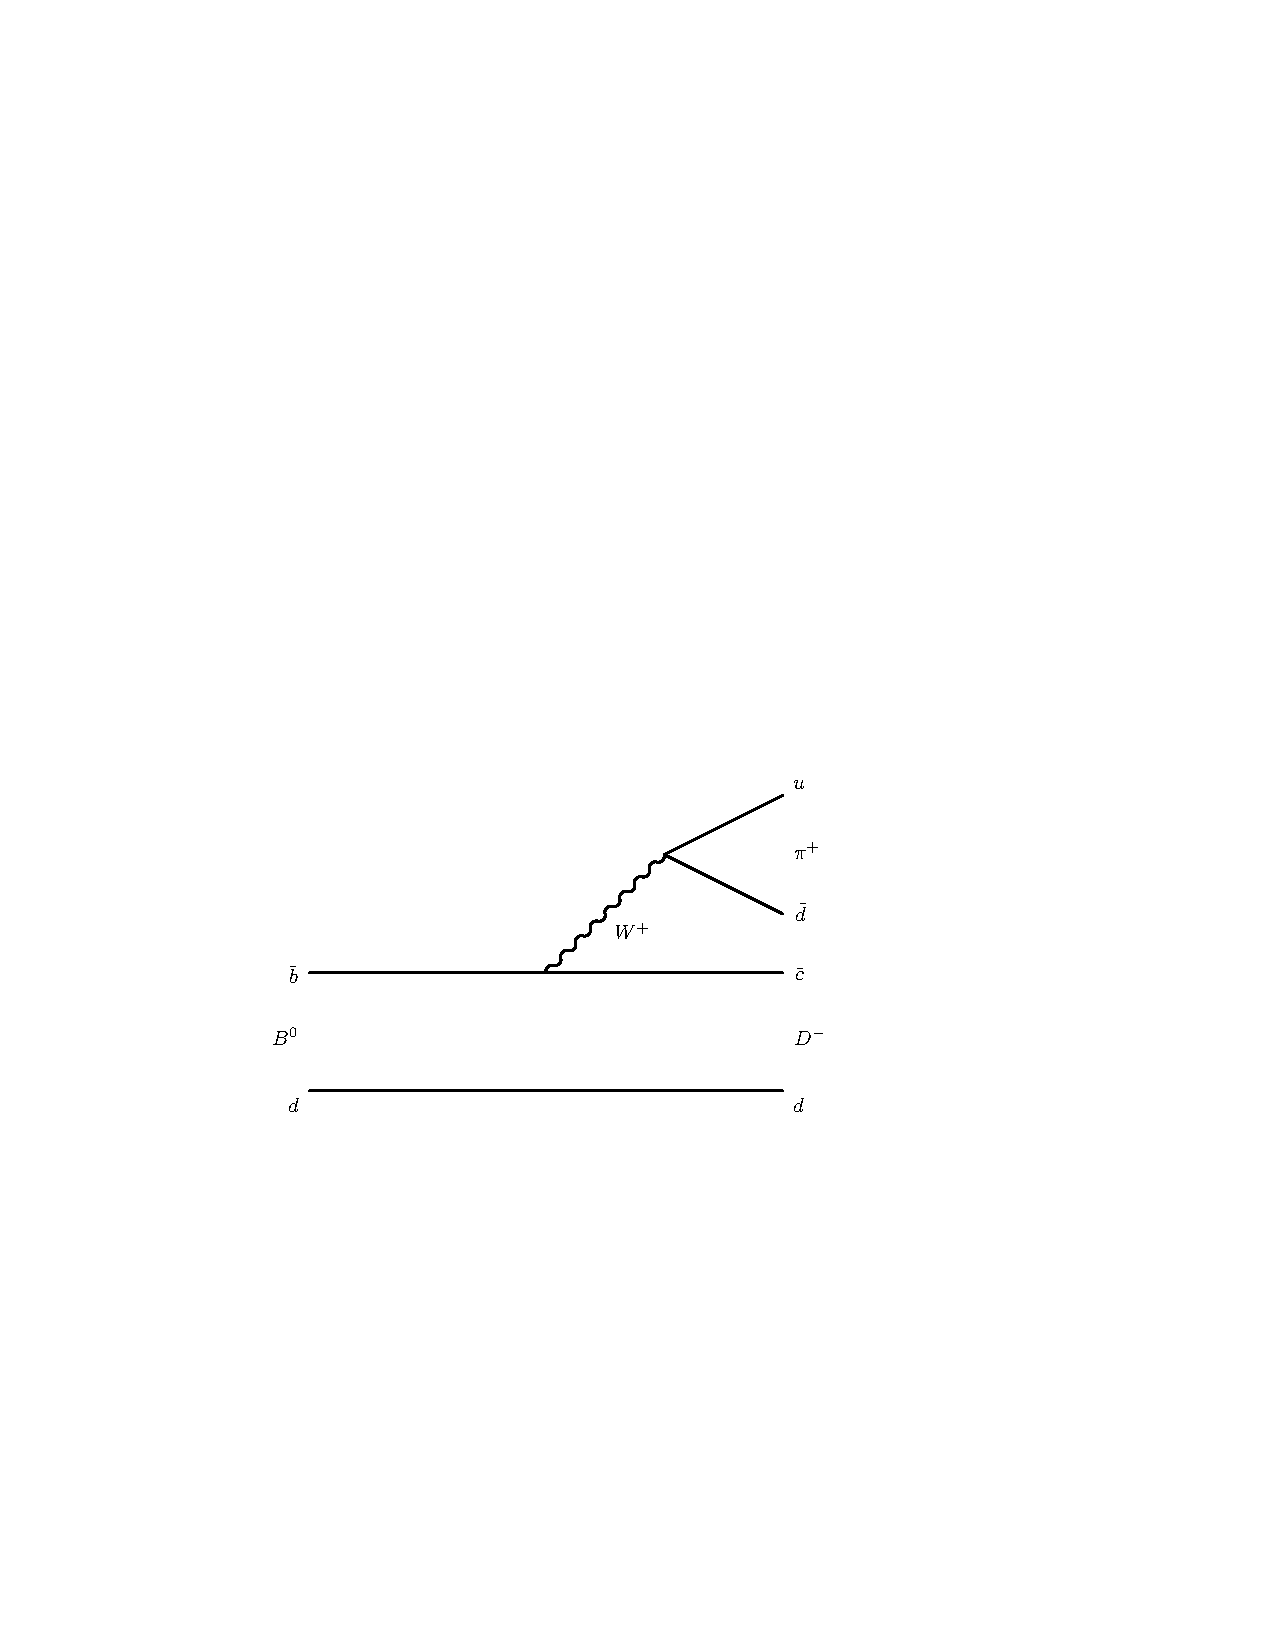
\includegraphics[width=0.45\textwidth]{fig/B2D-pi+.pdf}
		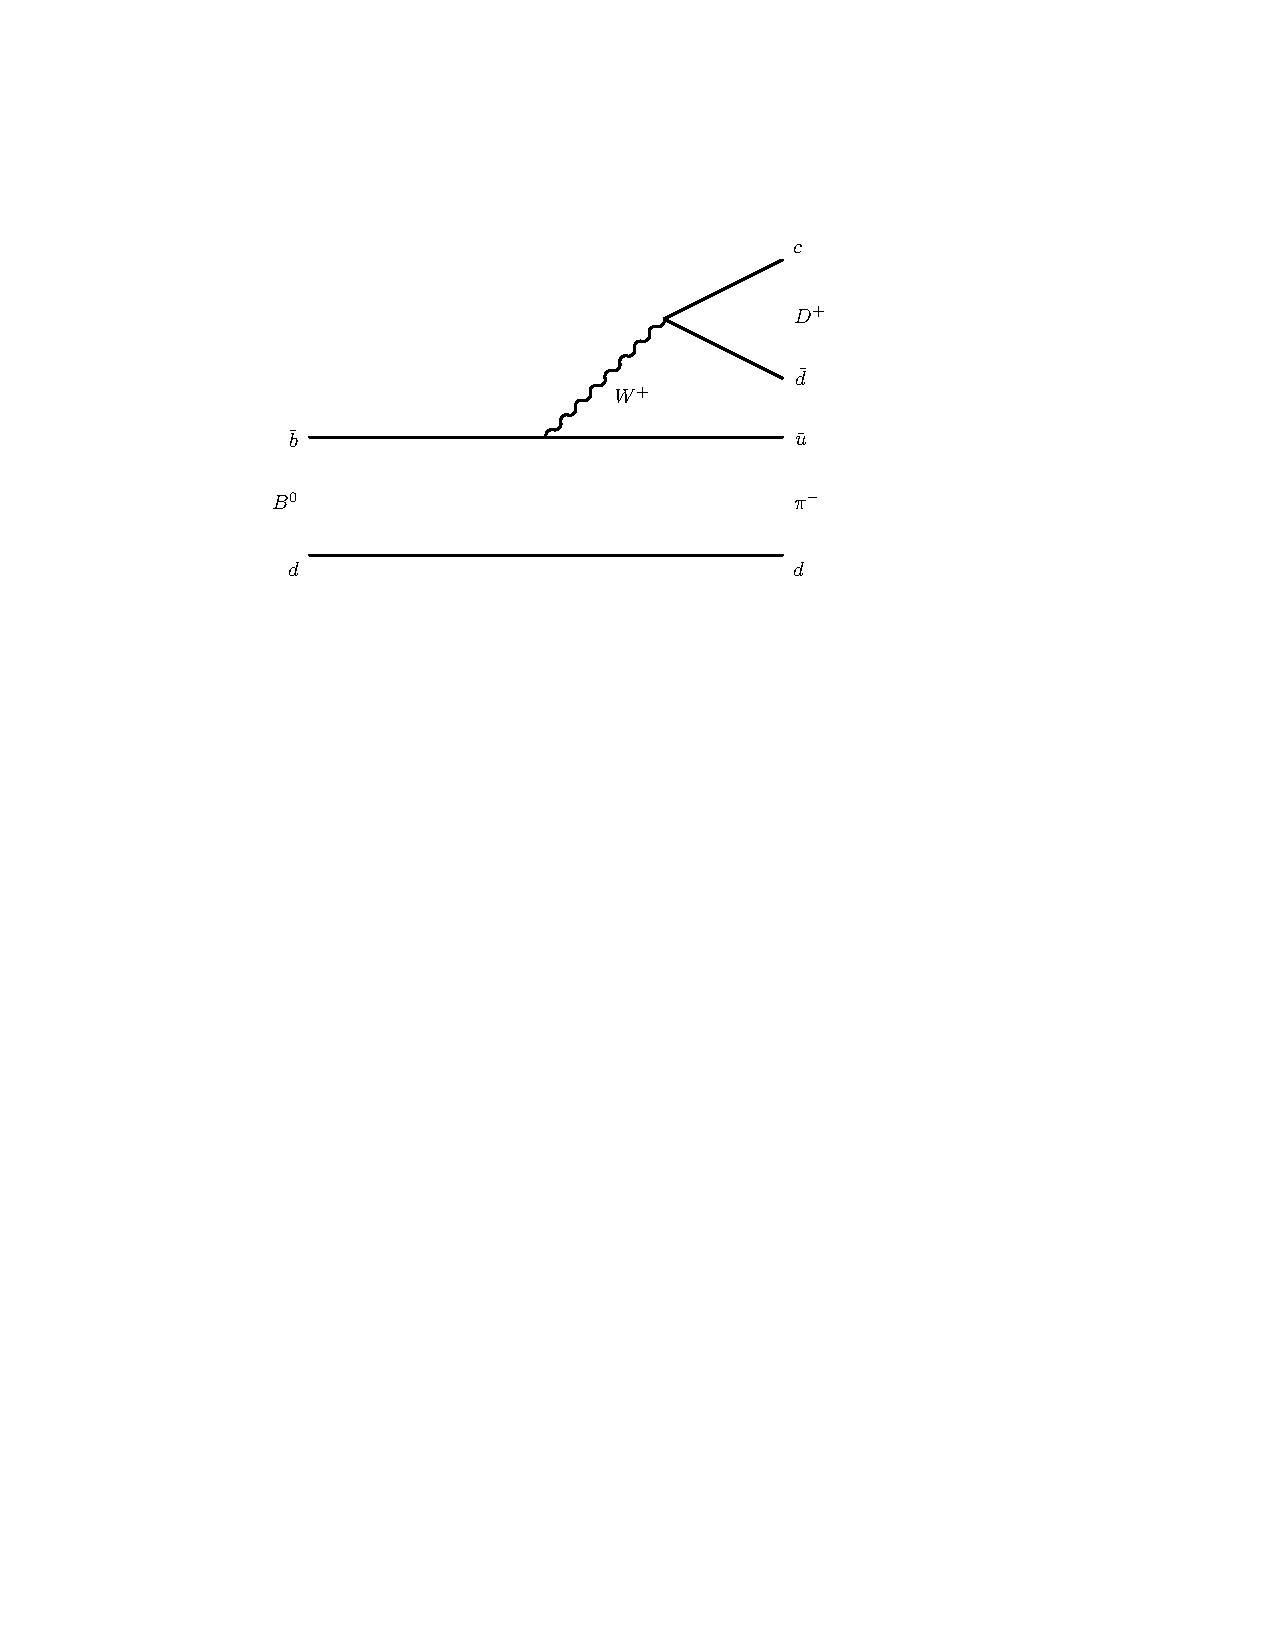
\includegraphics[width=0.45\textwidth]{fig/B2D+pi-.pdf}
	\caption{Feynmandiagramme der beiden Zerfälle des neutralen \B-Mesons in geladene $D\pi$ Endzustände. Rechts der Zerfall $\Bz\rightarrow D^+\pim$, der gegenüber dem in dieser Arbeit betrachtete Zerfall $\Bz\rightarrow \Dm\pip$ $C\!K\!M$ unterdrückt ist.}
	\label{fig:b2dpi} 
\end{figure}  
Im Kanal $\Bz\rightarrow \Dm\pip$ ist die Zerfallsamplitude proportional zu $\Vud\Vcb\propto\lambda^2$, im Kanal $\Bz\rightarrow D^+\pim$ jedoch nur zu $\Vub\Vcd\propto\lambda^4$ (siehe Gleichung \eqref{eq:wolfen}), sodass dieser zweite Kanal $C\!K\!M$ unterdrückt ist. Aus diesem Grund lässt sich $\Bz\rightarrow \Dm\pip$ trotzdem zur Kalibrierung des Flavour Taggings nutzen. Allerdings muss beachtet werden, dass Einflüsse des $C\!K\!M$ unterdrückten Zerfalls einen Einfluss auf die Messung der mistags $\omega$ haben kann. \\
Der Zerfall $\Bz\rightarrow \Dm\pip$ wird im Folgenden aus dem weiteren Zerfall $\mbox{\Dm\rightarrow \Kp\pim\pim}$ und einem geladenen Tochter Pion rekonstruiert.

\section{Selektion}\label{sec:selektion}

Für die Rekonstruktion von Ereignissen mit dem Zerfall $\Bz\rightarrow \Dm\pip$ werden vier HLT Trigger verwendet, drei sogenannte Topo Trigger und eine inklusiver $\phi$ Trigger. Die Topo Trigger fordern gut rekonstruierte Kandidaten mit einem Sekundärvertex aus zwei, drei oder vier Spuren. Für die inklusiven $\phi$ Trigger muss ein geladenes Kaon im Endzustand sein, da dass $\phi$  in etwa \SI{50}{\%} aller Fälle in zwei geladene Kaonen zerfällt. 
\begin{table}[tbp]
  \centering
     \caption{Schnitte der Vorselektion für den Kanal $\Bz\rightarrow \Dm\pip$ in der Stripping Version 20. Abweichende Schnitte für die Version 20r1 sind in Klammern gegeben.}
    \label{tab:stripping}
    \begin{tabular}{cc}
    \toprule
    \multicolumn{2}{c}{Schnitte auf \Bz-Kandidaten} \\
    \midrule
    Summe der Transversalimpulse \pt aller Teilchen & $>\SI{5000}{MeV\per c}$\\
    $\chi^2$ des Primär Vertex & $<25$ \\
    Primär Vertex $\chi^2/\text{ndof}$ & $<10$\\
    cos von $\sphericalangle\left[\left|PV,\Bz\text{Vtx}\right|, \vec{p}\left(\Bz\right)\right]$ & $<0{,}999$ \\
    Zerfallszeit & $>\SI{0{,}2}{ps}$\\
    $m\left(\kaon\pion\pion\pion\right)_\text{min}$ & \SI{4750}{MeV\per c^2}\\
    $m\left(\kaon\pion\pion\pion\right)_\text{max}$ & \SI{6000}{MeV\per c^2}\\ 
    \midrule
    \multicolumn{2}{c}{Schnitte auf \Dm-Kandidaten}\\ 
    \midrule
    Summe der Transversalimpulse \pt aller Teilchen & $>\SI{1800}{MeV\per c}$\\
    Vertex $\chi^2/\text{ndof}$ & $<10$\\
    bestes $\chi^2$ des Primär Vertex & $>36$\\
    cos von $\sphericalangle\left[\left|PV,\Dm\text{Vtx}\right|, \vec{p}\left(\Dm\right)\right]$ & $>0$ \\
    Maximaler Abstand der kleinsten Annäherung zum PV & $<\SI{0{,}5}{mm}$\\ 
    \midrule
    \multicolumn{2}{c}{Schnitte auf \Kp- und \pipm-Kandidaten}\\ 
    \midrule
    Transversalimpuls \pt & $>\SI{100}{MeV\per c}$\\
    Impuls $p$ & $>\SI{1000}{MeV\per c}$\\
    $\chi^2/\text{ndof}$ der Spur & $<3$\\
    ghost-Wahrscheinlichkeit der Spur & $<0{,}3$ ($<0{,}4$) \\
    kleinstes Stoßparameter $\chi^2$ & $>4$\\ 
    \bottomrule
    \end{tabular}
\end{table}
Obwohl der Zerfall $\Bz\rightarrow \Dm\pip$ kein $\phi$ enthält ist, ist dieser Trigger aufgrund des geladenen Kaons im Zerfall des \D-Mesons $\Dm\rightarrow \Kp\pim\pim$ geeignet.\\
Bei der weiteren Vorselektion, dem sogenannten Stripping, werden die Schnitte aus Tabelle \ref{tab:stripping} angewendet. Dabei wird zwischen den Jahren 2011 und 2012 mit den Stripping Versionen 20r1 und 20 unterschieden. Die finale Selektion wurde in Anlehnung an eine Analyse zur Messung der \Bs-Lebenszeit relativ zur \Bz-Lebenszeit entnommen \cite{selektion}. Sie unterteilt sich in einfache rechtwinklige Schnitte und speziellere Massen Vetos, um bestimmte nicht flache (peakende) Untergründe auszuschließen. Außerdem wurde in jedem Ereignis nur der Zerfall mit dem am besten rekonstruierten PV gewählt. Die rechtwinkligen Schnitte sind in Tabelle \ref{tab:selektion} zu sehen.
\begin{table}[tbp]
  \centering
     \caption{Rechtwinklige Schnitte der finalen Selektion.}
    \label{tab:selektion}
    \begin{tabular}{cc}
    \toprule
    \multicolumn{2}{c}{Schnitte auf \Bz-Kandidaten} \\ 
    \midrule
    größtes $\chi^2$ des Stoßparameters mit dem assoziierten PV & $<16$  \\ 
    cos von $\sphericalangle\left[\left|PV,\Bz\text{Vtx}\right|, \vec{p}\left(\Bz\right)\right]$ & $<0{,}9999$ \\
    Zerfallszeit & $>\SI{0{,}3}{ps}$\\ 
    $m\left(\kaon\pion\pion\pion\right)_\text{min}$ & \SI{5200}{MeV\per c^2}\\
    $m\left(\kaon\pion\pion\pion\right)_\text{max}$ & \SI{5500}{MeV\per c^2}\\ 
    \midrule   
    \multicolumn{2}{c}{Schnitte auf \Dm-Kandidaten} \\ 
    \midrule
    Zerfallszeit  & $>\SI{0}{fs}$  \\ 
    kleinstes $\chi^2$  der Flugdistanz mit dem SV & $>1$  \\ 
    kleinstes $\chi^2$ des Stoßparameters mit dem \Bz-PV & $>4$  \\ 
    $\left|m(\kaon\pion\pion)-m(\Dpm)_\text{PDG}\right|$ & $<\SI{25}{MeV \per c^2}$  \\
    \midrule
    \multicolumn{2}{c}{Schnitte auf \pip-Kandidaten} \\ 
    \midrule
    ist Myon & $=0$ \\ 
    kleinstes $\chi^2$ des Stoßparameters mit dem PV & $>36$  \\
    \dllkpi & $<2$  \\ 
    \midrule
    \multicolumn{2}{c}{Schnitte auf \Kp- und \pim-Kandidaten} \\ 
    \midrule
    kleinstes $\chi^2$ des Stoßparameters mit dem assoziierten PV & $>9$ \\
    \dllkpi für Pionen & $<5$  \\
    \dllkpi für \Kp & $>0$  \\ 
    \bottomrule
    \end{tabular}
\end{table}
Insgesamt erhält man nach allen rechtwinkligen Schnitten eine Signaleffizienz von \SI{73{,}24}{\%}. Bei den Massenvetos wurde auf zwei Untergründe eingegangen. Mit dem \Dsm-Veto soll der Zerfall $\Bs\rightarrow\Dsm\pip$ ausgeschlossen werden, das \Lc-Veto soll den Zerfall $\Lb\rightarrow\Lc\pim$ eliminieren:
\begin{figure}[tbp]
	\centering
		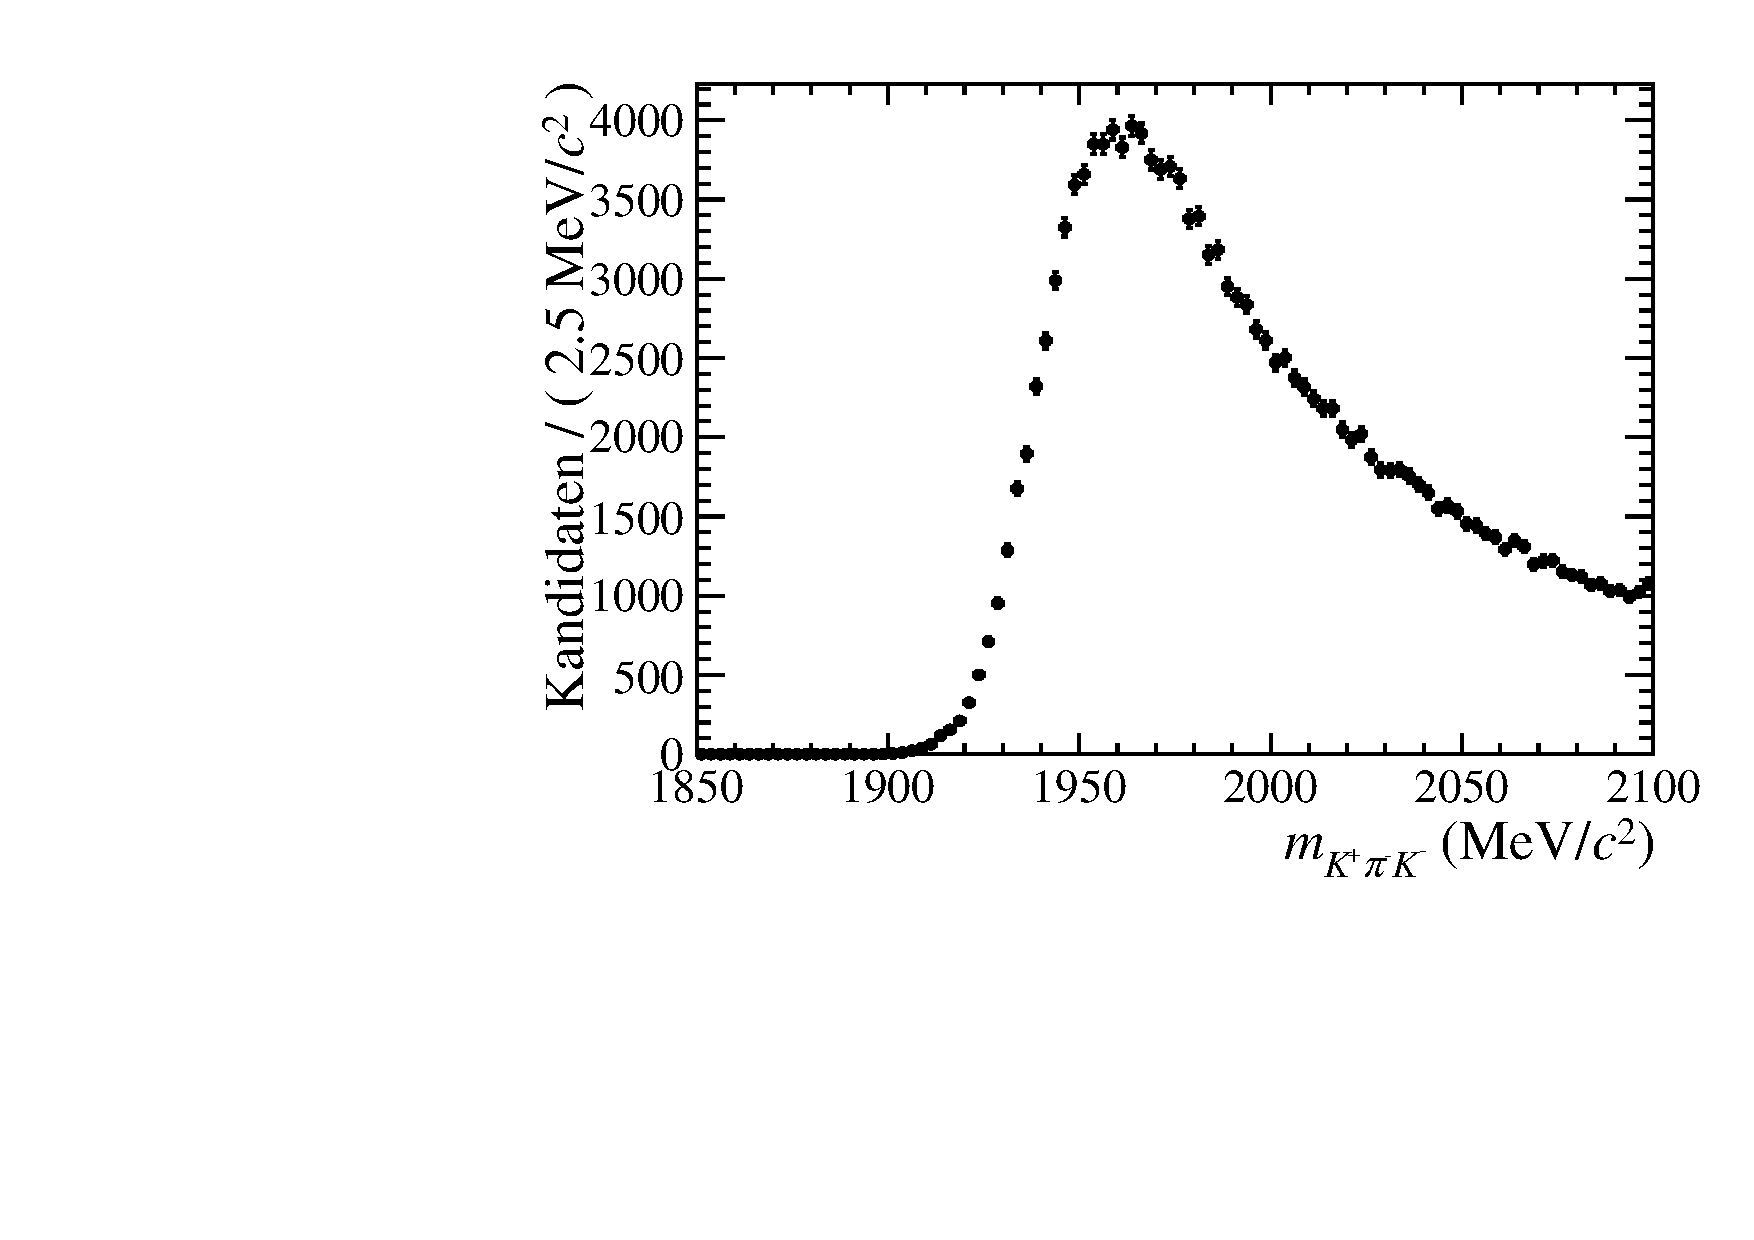
\includegraphics[width=0.45\textwidth]{fig/obsMass_Ds1.pdf}
		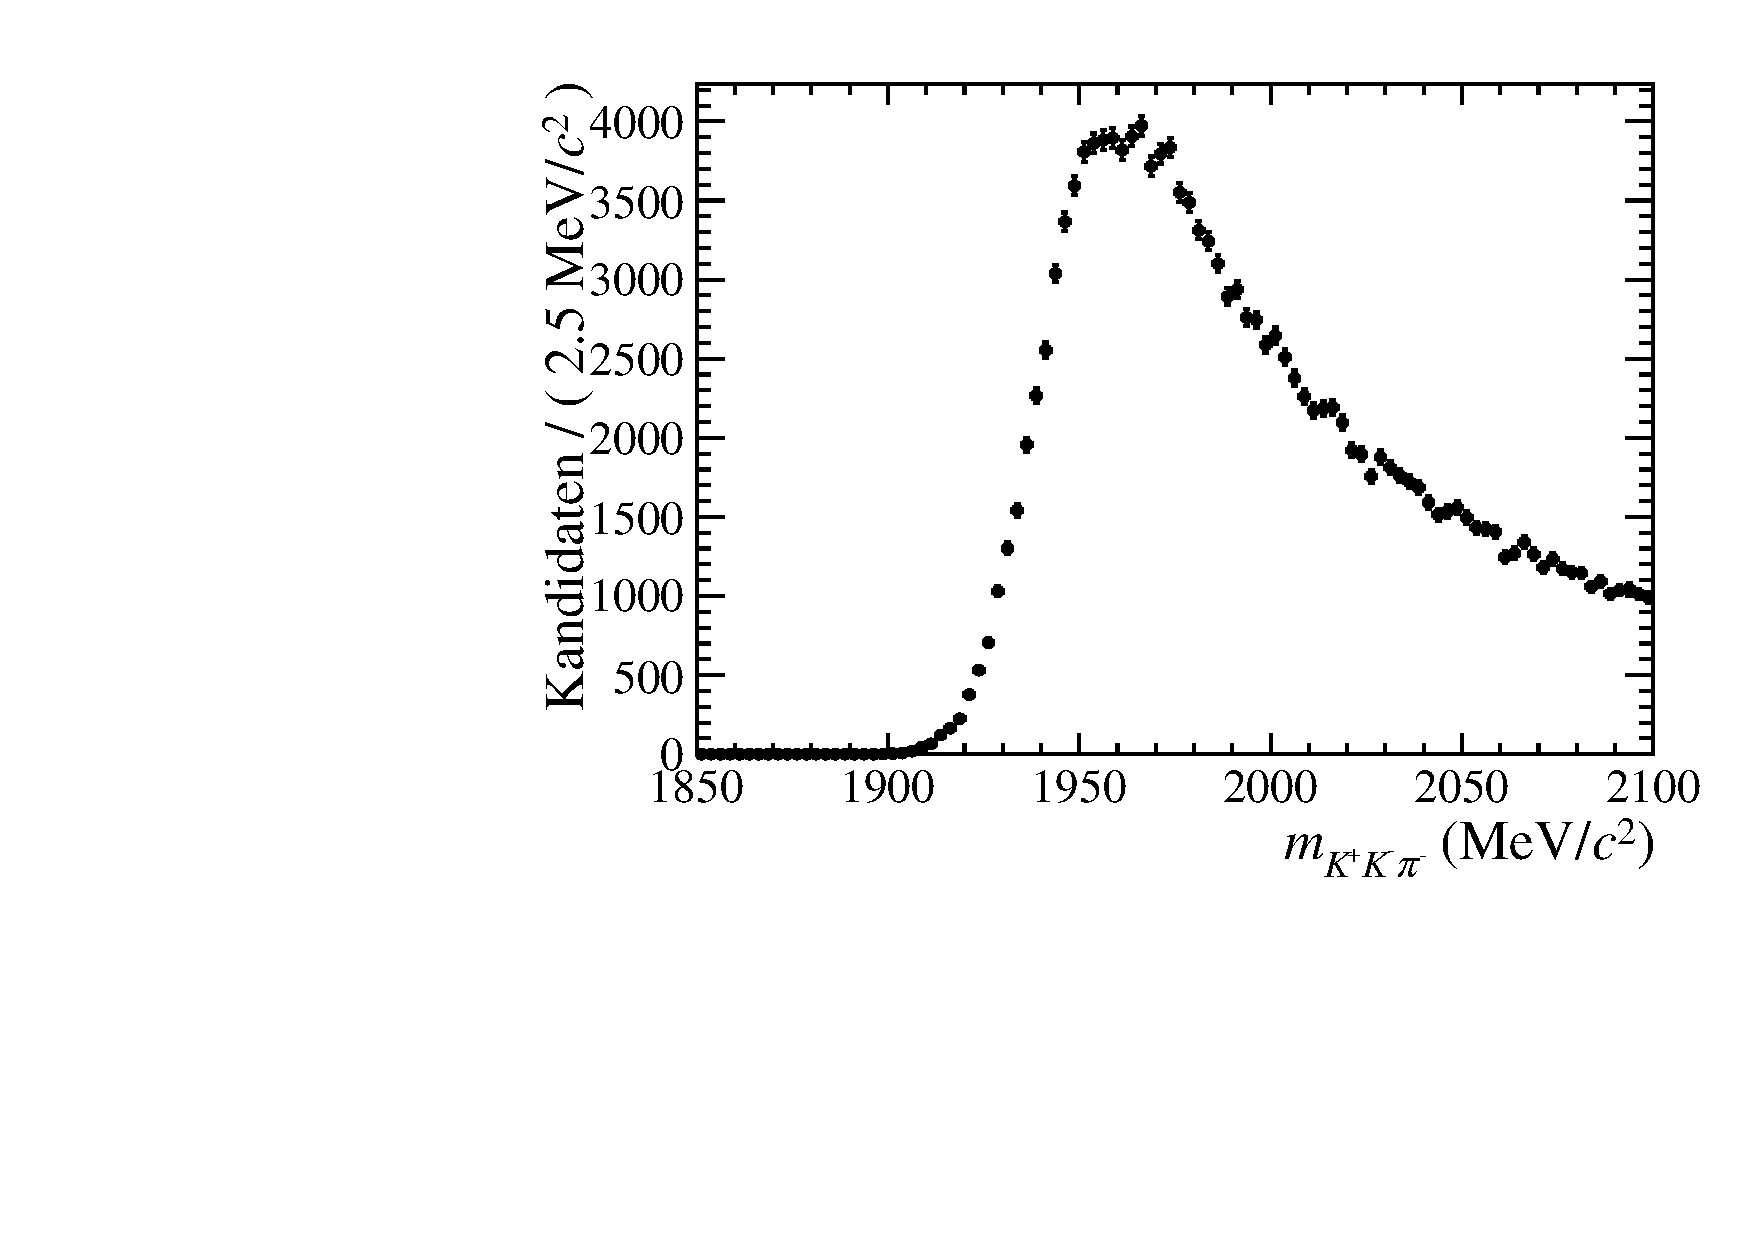
\includegraphics[width=0.45\textwidth]{fig/obsMass_Ds2.pdf}
	\caption{Massenverteilung der \Kp\pim\pim Kombination nach einer Kaon Massenhypothese für ein \pim. Die Plots entsprechen den Massenverteilungen für die zwei möglichen Kombinationen.}
	\label{fig:dsveto} 
\end{figure} 
\begin{figure}[tbp]
	\centering
		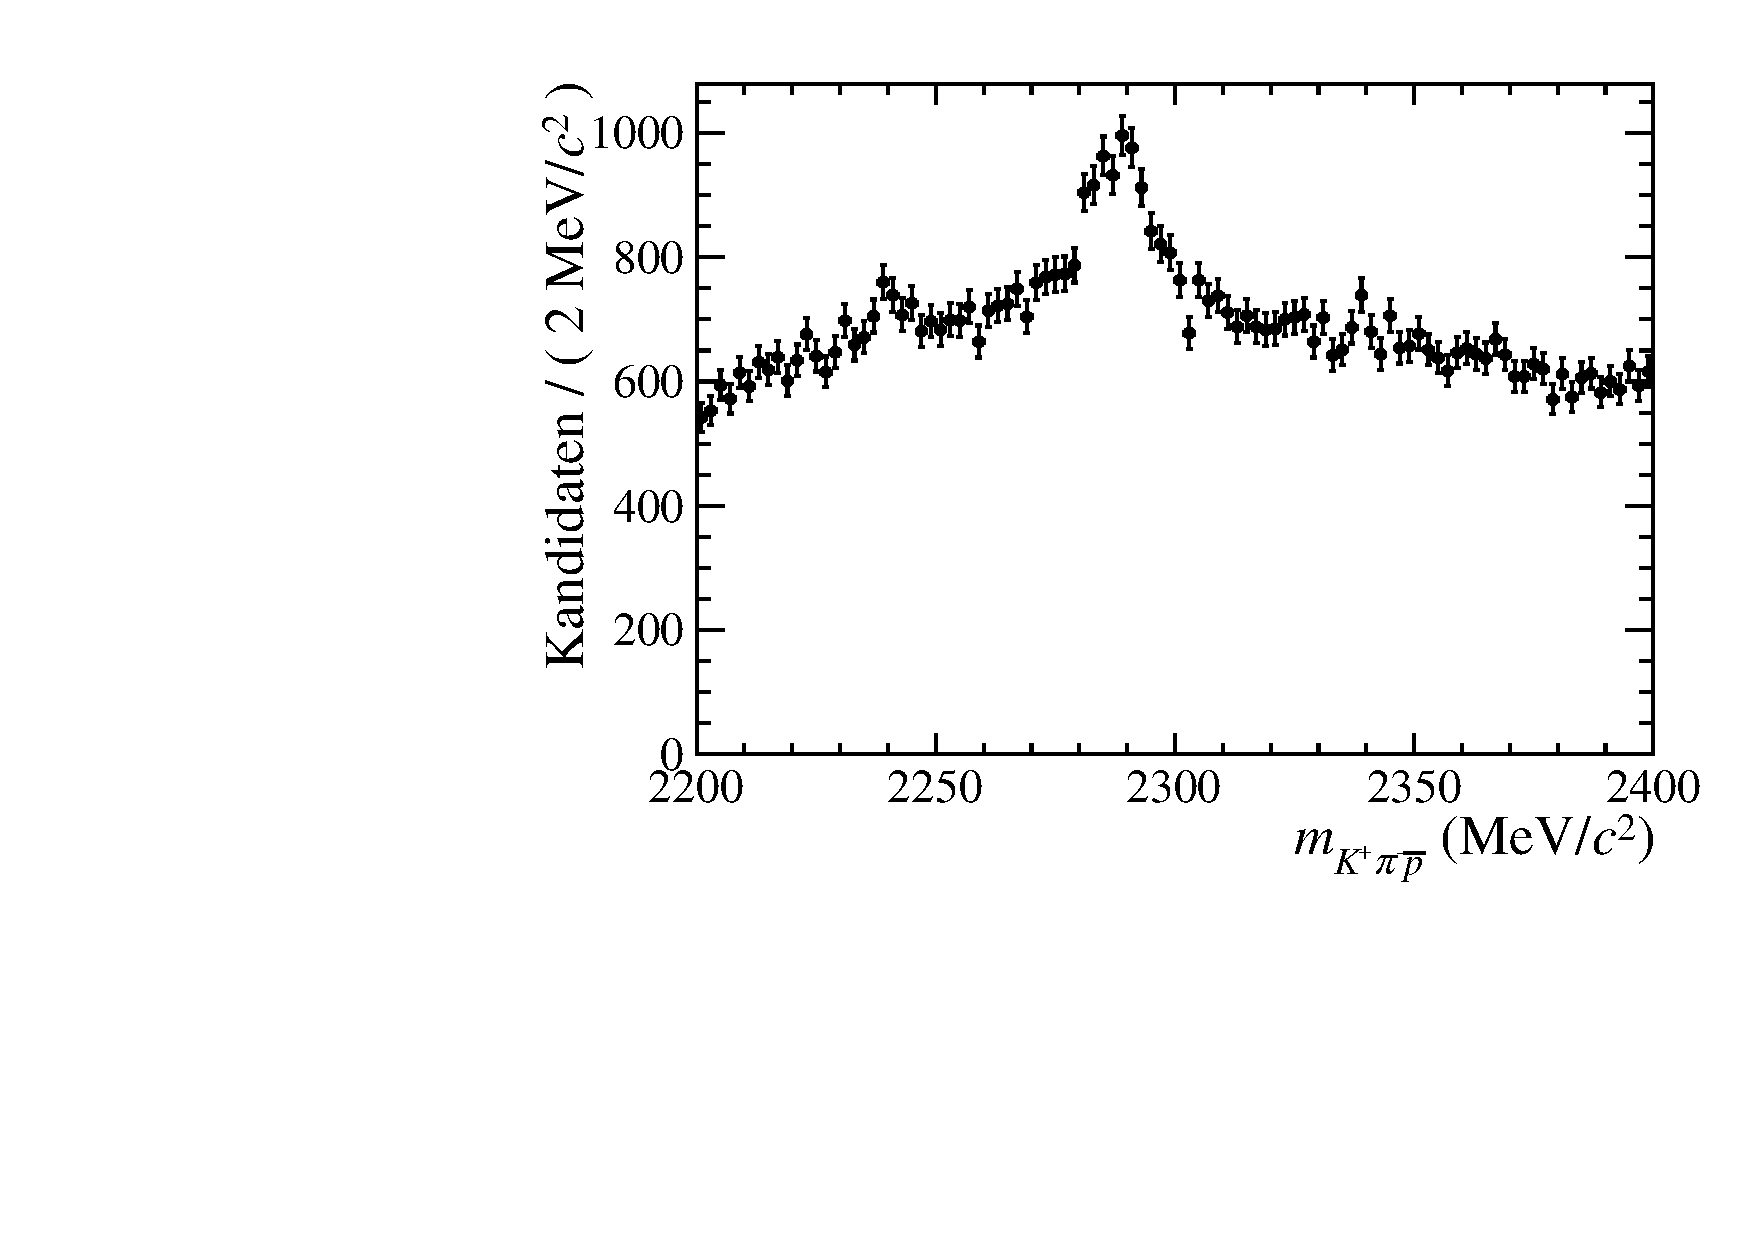
\includegraphics[width=0.45\textwidth]{fig/obsMass_lambda1.pdf}
		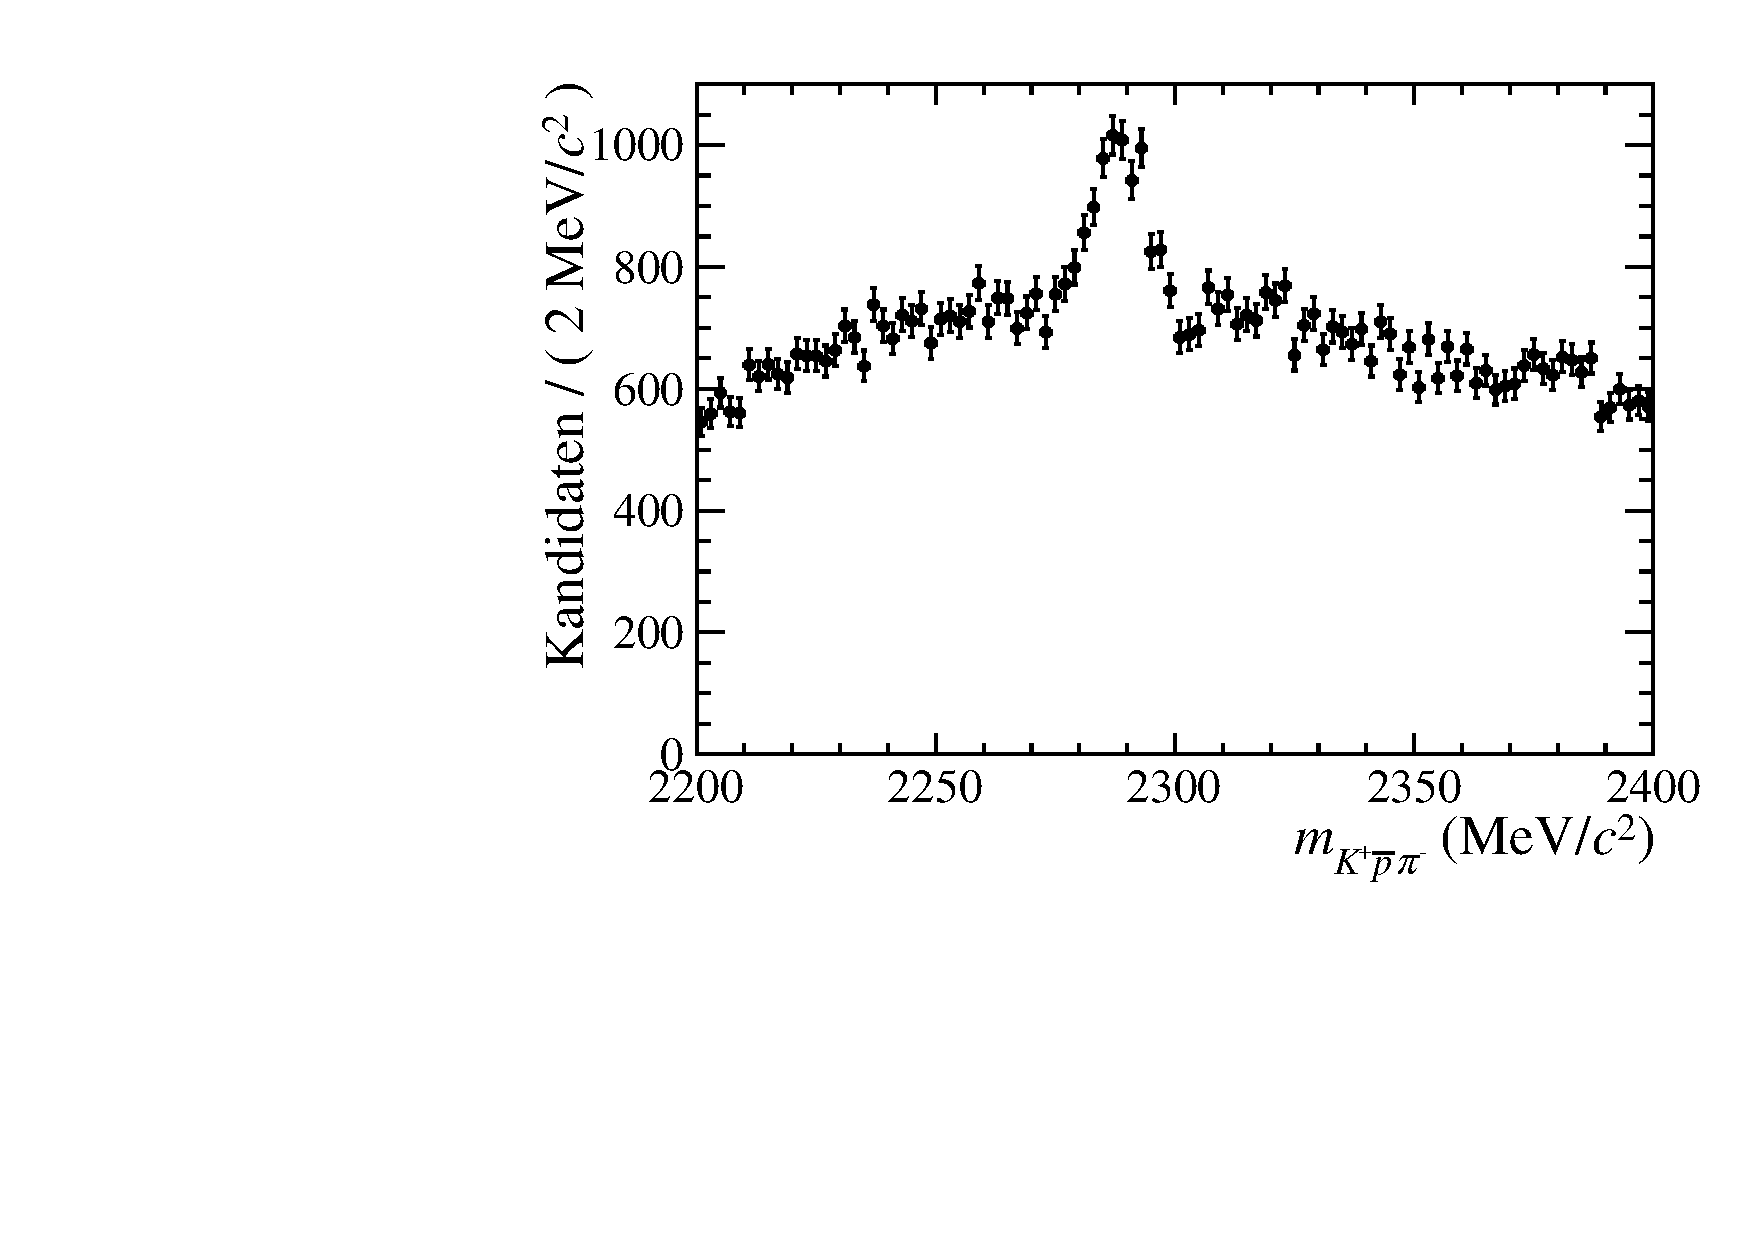
\includegraphics[width=0.45\textwidth]{fig/obsMass_lambda2.pdf}
	\caption{Massenverteilungen der \Kp\pim\pim Kombination nach einer Proton Massenhypothese für ein \pim. Die Plots entsprechen den Massenverteilungen für die zwei möglichen Kombinationen.}
	\label{fig:lcveto} 
\end{figure}  
\begin{itemize}
\item Bei dem \Dsm-Veto wird das \Kp mit einem den beiden \pim kombiniert, wobei ein \pim als Kaon fehlidentifiziert wurde. Es wird also nach dem Zerfall $\Dsm\rightarrow\Kp\Km\pim$ gesucht, um einen ähnlichen Endzustand zu bilden wie für das eigentlich gesuchte \Dm-Meson. In Abbildung \ref{fig:dsveto} sind die peakenden Massenverteilungen nach den Kaon Massenhypothesen für die \pim zu sehen. Nach der Kaon Massenhypothese werden Ereignisse mit $\dllkpi>0$ für das jeweilige \pim oder mit einer invarianten Masse innerhalb eines Massenfensters von \SI{30}{MeV\per c^2} um den zentralen Wert der \Dsm-Masse weg geschnitten. Dabei beschreibt \dllkpi die Wahrscheinlichkeit ob es sich bei einem Teilchen eher um ein Pion oder ein Kaon handelt.
\item Für das \Lc-Veto werden das Kaon und die beiden negativ geladenen Pionen kombiniert, wobei eines der \pim mit einer Proton Massenhypothese versehen wird. Hier soll für das \Lc der Zerfall $\Lc\rightarrow\Km\pip\proton$ gesucht werden. Die peakenden Massenverteilungen nach der Proton Massenhypothese sind in Abbildung \ref{fig:lcveto} zu sehen. Im Folgenden werden nur Ereignisse beachtet, bei denen für das \pim mit der Protonmassenhypothese entweder $\dllppi<0$ gilt oder die Kombination aus \Kp, \pim und \pim mit der Proton Massenhypothese für ein \pim muss außerhalb eines Massenfensters von \SI{30}{Mev\per c^2} um den zentralen Wert der \Lc-Masse sein. Die Größe \dllppi beschreibt hier für ein Teilchen die Wahrscheinlichkeit, ob es sich eher um ein Proton oder Pion handelt.
\end{itemize}
Nach Anwendung aller Schnitte und der beiden Massenvetos ergibt sich eine Signaleffizienz von \SI{67{,}83}{\%} auf Monte Carlo. Diese Signaleffizienz ist für ein Signal Monte Carlo für das Jahr \num{2011} berechnet.
 
\section{Verwendetes Fitmodell}

Das Fitmodell für den Kanal $\Bz\rightarrow\Dm\pip$ setzt sich aus einer Signal und einer Untergrund Komponente zusammen. Die \mbox{Wahrscheinlichkeitsdichtefunktion $\mathcal{P}$ (\PDF)} hat daher die folgende Form:
\begin{equation}
N\mathcal{P}(t,\xi,m;\vec{\zeta})=N_\text{Sig}\mathcal{P}_\text{Sig}(t,\xi,m;\vec{\zeta}_\text{Sig})+N_\text{Bkg}\mathcal{P}_\text{Bkg}(t,m;\vec{\zeta}_\text{Bkg}).
\end{equation}
Dabei stellen $m$, $t$ und $\xi$ die beobachteten Observablen (Masse, Zeit und Mischungszustand der \Bz-Mesonen) dar und die $N$ geben die Ereigniszahlen an. Der Mischungszustand ist dabei definiert als $\xi=d\cdot d_f$ mit dem Tag $d$ und dem Zerfallszustand $d_f$. Hat ein \Bz-Meson gemischt ist $\xi=-1$, für ungemischte \Bz-Mesonen gilt $\xi=1$ und bei ungetaggten Ereignissen ist $\xi=0$. Die Signal- (Sig) und Untergrundkomponenten (Bkg) setzen sich weiter als Produkt aus einer \PDF für die Zerfallszeit und für die Masse zusammen
\begin{equation}
\begin{split}
\mathcal{P}_\text{Sig}(t,\xi,m;\vec{\zeta}_\text{Sig})&=\mathcal{P}_\text{Sig,Zeit}(t,\xi;\vec{\zeta}_\text{Sig})\cdot\mathcal{P}_\text{Sig,Masse}(m;\vec{\zeta}_\text{Sig})\\
\mathcal{P}_\text{Bkg}(t,m;\vec{\zeta}_\text{Bkg})&=\mathcal{P}_\text{Bkg,Zeit}(t,\xi;\vec{\zeta}_\text{Bkg})\cdot\mathcal{P}_\text{Bkg,Masse}(m;\vec{\zeta}_\text{Bkg})
\end{split}
\end{equation}
und sollen im Folgenden näher beschrieben werden.

\subsection{Zerfallszeit Beschreibung}

Die Wahrscheinlichkeitsdichtefunktion zur Beschreibung der Zerfallszeit leitet sich direkt aus den Übergangswahrscheinlichkeiten aus Abschnitt \ref{sec:mixing} ab. Dabei wird eine mögliche \CP-Verletzung in der Mischung vernachlässigt und für beide Masseneigenzustände eine gleiche Zerfallsbreite angenommen. Die vier möglichen Fälle lassen sich schließlich mit der Tagentscheidung $d$ und dem Mischungszustand $\xi$ zusammenfassen zu
\begin{equation}
\mathcal{P}'_\text{Sig,Zeit}(t,\xi;\tau,\dmd,\omega,\Delta\omega,d)\propto e^{-t/\tau}\left[\left(1-d\Delta\omega\right)+\xi\left(1-2\omega\right)\cos\left(\dmd t\right)\right]
\end{equation}
Für die Beschreibung des Untergrundes in der Zeitkomponente wird die \PDF 
\begin{equation}
\mathcal{P}'_\text{Bkg,Zeit}(t,\xi;\tau_\text{Bkg},\omega_\text{Bkg})\propto e^{-t/\tau_\text{Bkg}}\cdot\xi\left(1-2\omega_\text{Bkg}\right)
\end{equation}
genutzt. Der Parameter $\omega_\text{Bkg}$ beschreibt eine mögliche Asymmetrie für \Bz- und \Bzb-Mesonen im Untergrund. Neben diesen aus dem Modell des \B-Mesonenzerfalls motivierten Anteilen der Zerfallszeitbeschreibung gibt es allerdings noch zwei weitere  Effekte. \\ 
Zunächst wird die Lebenszeitverteilung durch die Selektion des Zerfalls beeinflusst. Vor allem die HLT Trigger machen Schnitte auf den Stoßparameter des \Bz-Mesons, was kurze Zerfallszeiten beeinflusst. Diese Schnitte sind nötig, um den großen kombinatorischen Untergrund aus Pionen zu unterdrücken, der bei den Protonenkollisionen direkt am PV entsteht. Der auftretende Effekt wird dabei mit einer Funktion der Form
\begin{equation}
\epsilon(t)=\arctan\left(t^{a_3}e^{a_1t+a_2}\right)
\end{equation}
beschrieben. Hierbei handelt es sich nicht um ein physikalisches Modell, sondern einzig um eine gute Beschreibung des auftretenden Effekts. In Abbildung \ref{fig:akzeptanz} ist das Akzeptanzmodell und sein Einfluss auf die Lebenszeitverteilung dargestellt.
\begin{figure}[tbp]
	\centering
		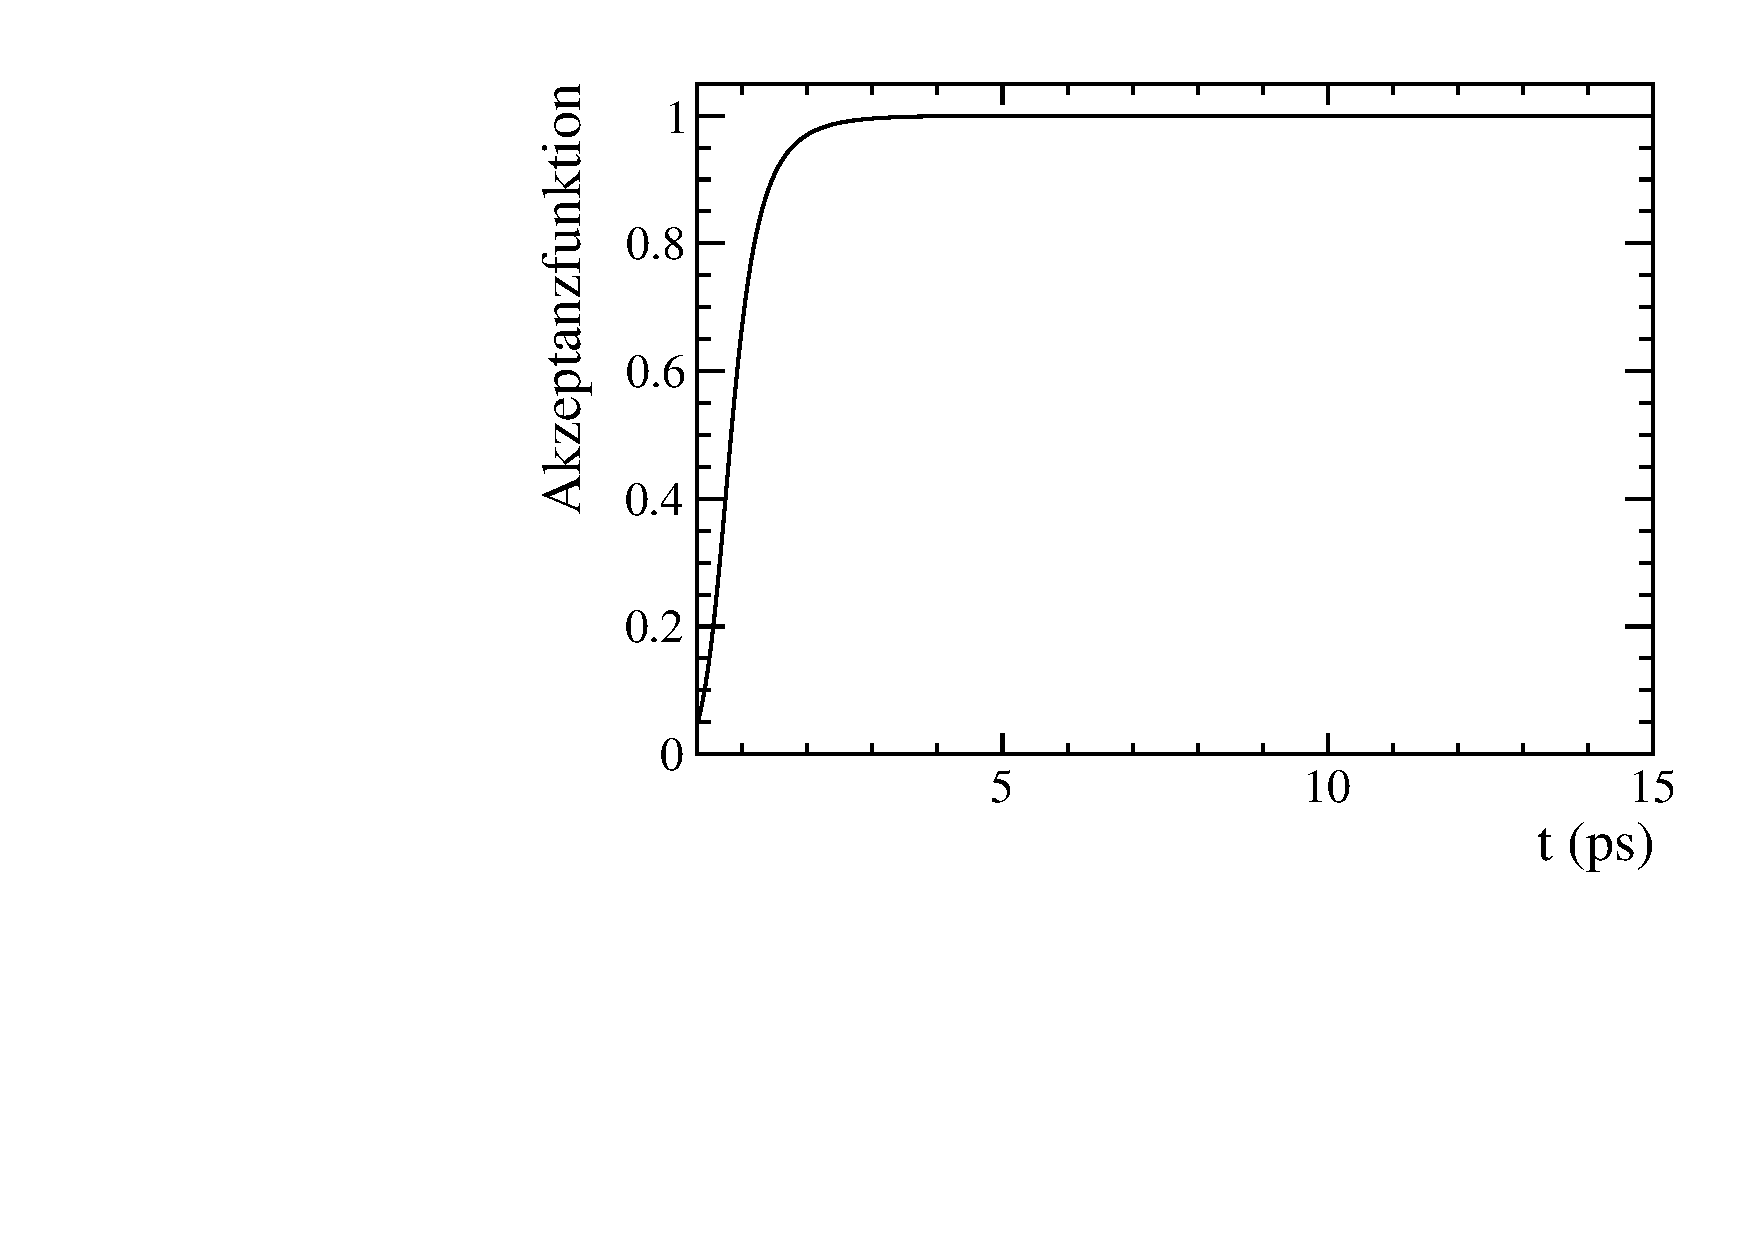
\includegraphics[width=0.45\textwidth]{fig/akzeptanz.pdf}
		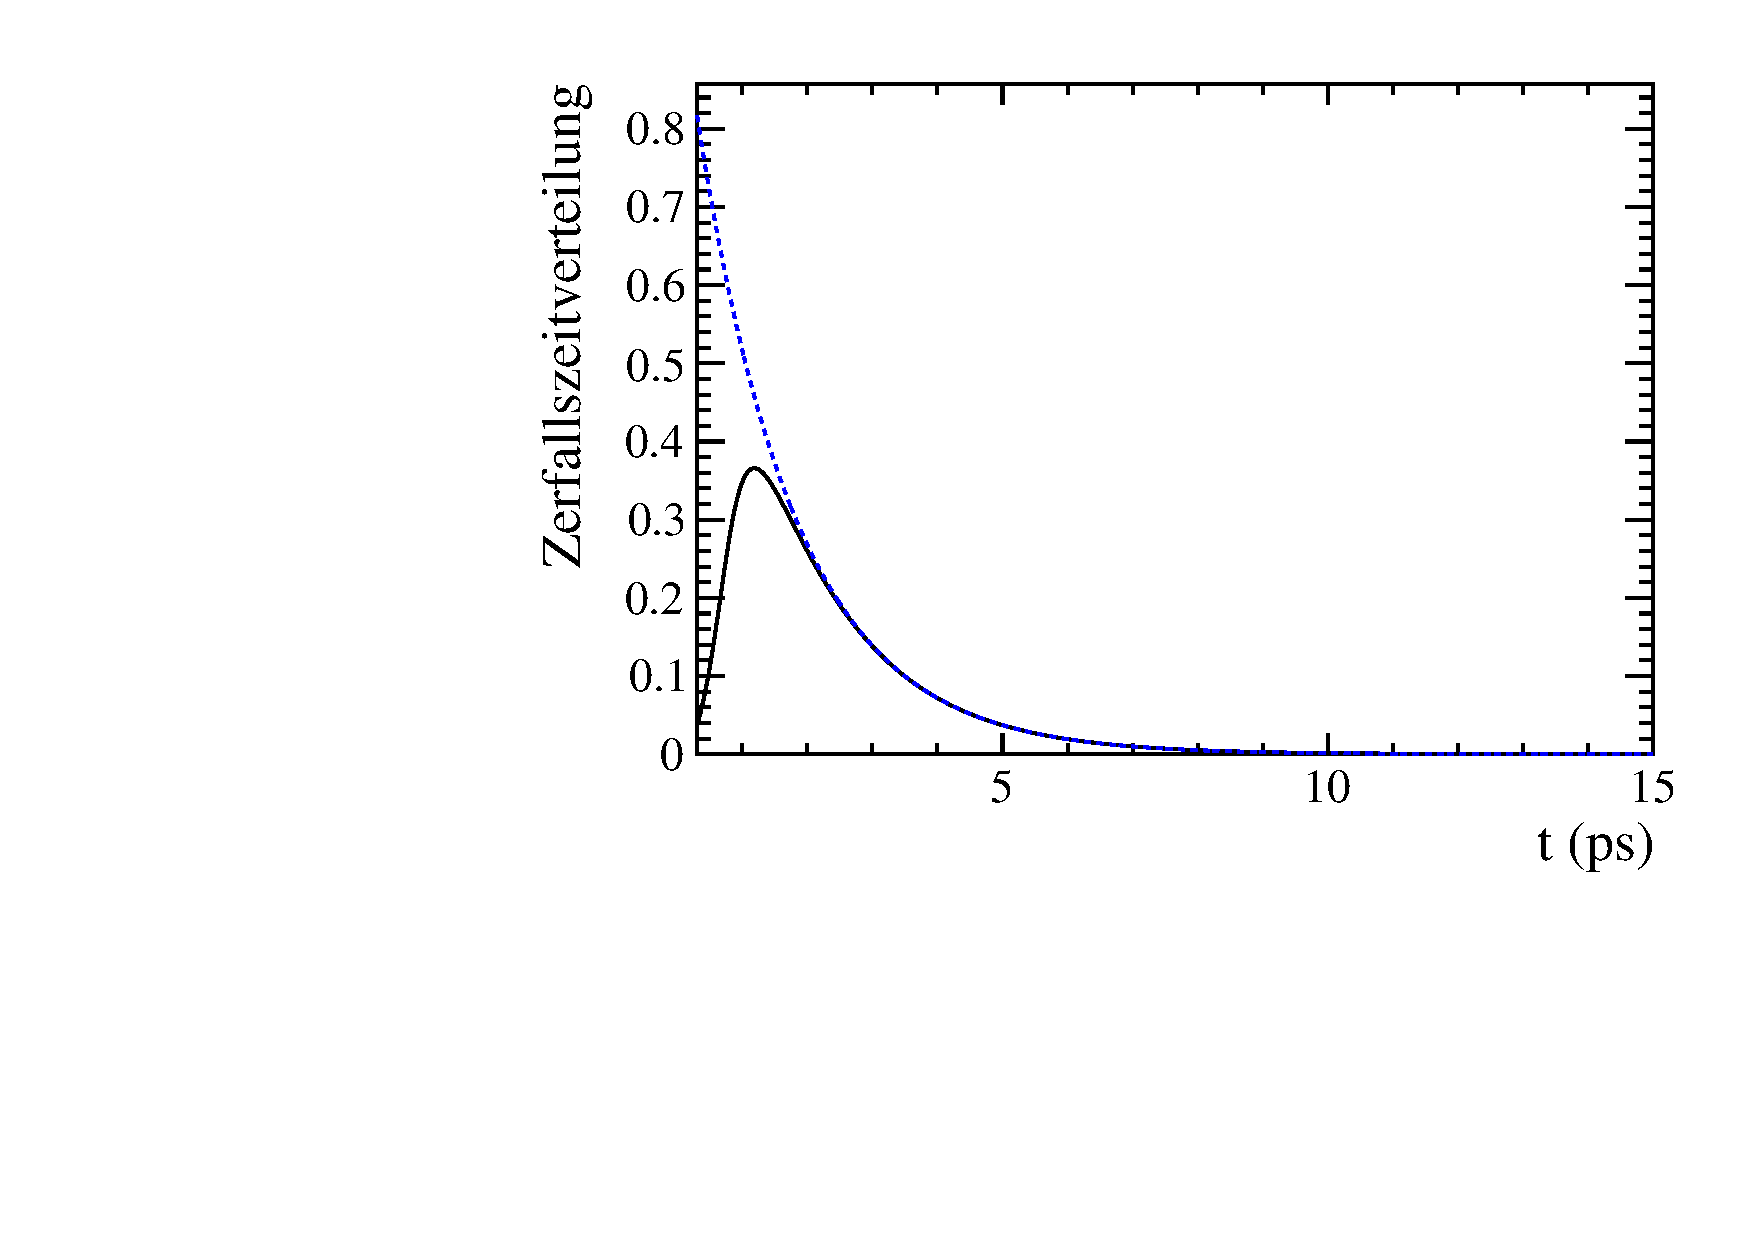
\includegraphics[width=0.45\textwidth]{fig/akzept_expo.pdf}
	\caption{Links die Akzeptanzfunktion die in $\Bz\rightarrow\Dm\pip$ genutzt wird, rechts der Einfluss auf die Zerfallszeitverteilung. In blau gestrichelt ohne und in schwarz mit Akzeptanzeffekt.}
	\label{fig:akzeptanz} 
\end{figure}
Dabei wurde für Signal und Untergrund das gleiche Modell mit  unterschiedlichen Werten für die Parameter $a_1$, $a_2$ und $a_3$ gewählt.\\
Der zweite Effekt, der zu beachten ist, ist die detektorbedingte Auflösung. Hier wurde für Signal und Untergrund das gleiche Modell einer einfachen gaussischen Auflösung 
\begin{equation}
\mathcal{R}(t-t_\text{wahr};s)\propto\frac{1}{s\sqrt{2\pi}}\exp\left(-\frac{\left(t-t_\text{wahr}\right)^2}{2s^2}\right)
\end{equation}
mit einer mittleren Auflösung von $s=\SI{50}{fs}$ verwendet.\\
Insgesamt erhält man so für die Zeitbeschreibung in Signal und Untergrund
\begin{equation}
\begin{split}
\mathcal{P}_\text{Sig,Zeit}(t,\xi;\vec{\zeta}_\text{Sig})&=\epsilon(t)\cdot\mathcal{P}'_\text{Sig,Zeit}(t,\xi;\tau,\dmd,\omega,\Delta\omega,d)\otimes\mathcal{R}(t-t_\text{wahr};s)\\
\mathcal{P}_\text{Bkg,Zeit}(t,\xi;\vec{\zeta}_\text{Bkg})&=\epsilon(t)\cdot\mathcal{P}'_\text{Bkg,Zeit}(t,\xi;\tau_\text{Bkg},\omega_\text{Bkg})\otimes\mathcal{R}(t-t_\text{wahr};s)
\end{split}
\end{equation}

\subsection{Massen Beschreibung}

Als Wahrscheinlichkeitsdichtefunktion für die Masse wurde eine Ipatia Funktion \cite{ipatia}
\begin{multline}
			\mathcal{I}(m;\mu,\sigma,\lambda,\zeta,\beta,a_1,n_1,a_2,n_2) \propto \\
			\begin{cases}
			\left(\left(m - \mu\right)^2 + A_{\lambda}^2(\zeta)\sigma^2\right)^{\frac{1}{2}\lambda - \frac{1}{4}} e^{\beta(m - \mu)} K_{\lambda - \frac{1}{2}}\left(\zeta\sqrt{1 + \left(\frac{m - \mu}{A_\lambda(\zeta)\sigma}\right)^2}\right)	&\, ,  - a_1 < \frac{m - \mu}{\sigma} < a_2 \\
			\frac{G(\mu - a_1 \sigma,\mu,\sigma,\lambda,\zeta,\beta)}{\left(1 - m/(n \frac{G(\mu - a_1\sigma,\mu,\sigma,\lambda,\zeta,\beta)}{G^\prime(\mu - a_1 \sigma,\mu,\sigma,\lambda,\zeta,\beta)} -a_1 \sigma)\right)^{n_1}}	&\, , - a_1 > \frac{m - \mu}{\sigma} \\
			\frac{G(\mu - a_2 \sigma,\mu,\sigma,\lambda,\zeta,\beta)}{\left(1 - m/(n \frac{G(\mu - a_2\sigma,\mu,\sigma,\lambda,\zeta,\beta)}{G^\prime(\mu - a_2 \sigma,\mu,\sigma,\lambda,\zeta,\beta)} -a_2 \sigma)\right)^{n_2}}	&,\quad a_2 < \frac{m - \mu}{\sigma} \\
			\end{cases}
			\label{eq:ipatia}
		\end{multline}
mit 
\begin{equation}
\begin{split}
&G(m,\mu,\sigma,\lambda,\zeta,\beta,a,n)\propto\\
&\left(\left(m-\mu\right)^2+A_\lambda^2(\zeta)\sigma^2\right)^{\frac{1}{2}\lambda-\frac{1}{4}}e^{\beta\left(m-\mu\right)}K_{\lambda-\frac{1}{2}}\left(\zeta\sqrt{1+\left(\frac{m-\mu}{A_\lambda(\zeta)\sigma}\right)^2}\right)
\end{split}
\end{equation}
benutzt. Dabei beschreibt $\mu$ den Mittelwert, $\sigma$ die Standardabweichung und die Parameter $a_i$ und $n_i$ mögliche exponentielle Ränder der Verteilung. Diese können entstehen, wenn beispielsweise durch Wechselwirkungen mit dem Magnetfeld Photonen emittiert werden (links) oder Detektoreffekte (rechts). Für den Untergrund wird eine Exponentialfunktion der Form
\begin{equation}
\Epsilon(m;M)\propto e^{\frac{m}{M}}
\end{equation}
gewählt um den kombinatorischen Untergrund zu beschreiben. Es ergibt sich also
\begin{equation}
\begin{split}
\mathcal{P}_\text{Sig,Masse}(m;\vec{\zeta}_\text{Sig})&=\mathcal{I}(m,\mu,\sigma,\lambda,\zeta,\beta,\alpha,n)\\
\mathcal{P}_\text{Bkg,Masse}(m;\vec{\zeta}_\text{Bkg})&=\Epsilon(m;M)\propto e^{\frac{m}{M}}.
\end{split}
\end{equation}

  % !TEX root = main.tex
\chapter{Kalibrierung verschiedener Tagger}

Im Folgenden Kapitel wird auf die Kalibrierung der unterschiedlichen Tagger eingegangen. Dazu wird zunächst die hier getroffene Auswahl der Tagger diskutiert, um daraufhin die einzelnen Kalibrierungen zunächst der OS Tagger und anschließend der SS Tagger zu betrachten. Anschließend werden die Ergebnisse in den aktuellen Stand des Flavour Taggings eingeordnet und diskutiert.  Zum Abschluss folgt eine Messung der Oszillationsfrequenz $\dmd$, sowie eine Kalibrierung der Standard OS Kombination nach der in Abschnitt \ref{sec:kalibrierungDaten} zusätzlich vorgestellten Methode, die Wahrscheinlichkeiten $P(\bquarkbar)$ zu verwenden.

\section{Auswahl der Tagger}

Im Rahmen dieser Arbeit werden nicht alle bei \lhcb existierenden Tagger im Hinblick ihrer Kalibrierung auf dem Kanal \BdToDpi untersucht. Das Hauptaugenmerk bei der Auswahl liegt auf den Neuentwicklungen, um bei diesen eine ersten, von den Entwicklern unabhängigen Gegenprobe, mit einer unabhängigen Selektion auf dem Kanal $\Bz\rightarrow D^-\pi^+$ durchzuführen. Der hier genannte Kanal ist dabei vor allem für den SS Pion BDT und den SS Proton Tagger von großem Interesse, da beide Algorithmen auf genau diesem entwickelt wurden. Weiter werden der OS Kaon nnet  und der OS Charm als weitere Neuentwicklungen untersucht. Zusätzlich zu den genannten Taggern werden außerdem die Kalibrierungen der Standardkombination der OS Tagger (OS Elektron, OS Myon, OS Kaon, OS Vertex Charge Tagger) und des SS Pion Tagger überprüft. Beide sind bereits in anderen Zerfallskanälen kalibriert worden, daher handelt es sich um eine Gegenprobe der Kalibrierung.\\
Für einen Überblick über die, bei den einzelnen Taggern, zur Verfügung stehende Statistik, sind die Anzahlen getaggter Signalkandidaten, sowie die gewählten Anzahlen an Kategorien der mistag-Wahrscheinlichkeit $\eta$ der genannten Tagger für die Jahre \num{2011} und \num{2012} in der Tabelle \ref{tab:anzahlen} dargestellt.
\begin{table}[htbp]
	\centering
	\caption{Anzahl an Kategorien der mistag-Wahrscheinlichkeit $\eta$ für die einzelnen Tagger für die Jahre \num{2011} und \num{2012}. In Klammern jeweils die Anzahl an getaggten Signalkandidaten.}
	\label{tab:anzahlen}
	\begin{tabular}{c|cc}
	\toprule
	& \multicolumn{2}{c}{$\#\eta$ Kategorien ($\#$ Signalkandidaten)}  \\
    	& 2011  & 2012 \\ 
	\midrule
  OS Std.-Kombination & 8 (53262) & 10 (133067)  \\
  OS Charm            & 5 (4699) & 5 (11319)  \\
  OS Kaon nnet        & 7 (64063) & 8 (161138)  \\
  SS Pion             & 6 (21116) & 7 (52533)  \\
  SS Pion BDT         & 7 (80780) & 8 (210678)  \\
  SS Proton           & 7 (48037) & 8 (113029)  \\ 
  \bottomrule
	\end{tabular}
\end{table}

\section{Kalibrierung der OS Tagger}

In diesem Abschnitt soll nun zunächst auf die Kalibrierung der OS Tagger eingegangen werden. Das Vorgehen zur Bestimmung der Zerfallszeitakzeptanz wird in alle Kanälen für die Daten beider Jahre gleich gewählt. Zunächst werden Gewichte nach dem \sPlot-Verfahren \cite{splot} berechnet, indem ein Massenfit an alle Kandidaten jedes Jahres gemacht wurde. Mit diesen Gewichten können in dem Datensatz dann die Signal- und einen Untergrundverteilungen getrennt werden. Für die Bestimmung der Akzeptanzparameter wird dann die Lebenszeit auf den Wertmittelwert $\tau=\SI{1{,}519}{ps}$ \cite{PDG-2012} festgesetzt, sodass nur die drei freien Parameter $a_1$, $a_2$ und $a_3$ bleiben. Im späteren zweidimensionalen Fit an Masse und Zeit werden diese Parameter dann auf die gefundenen Werte festgesetzt und die Lebenszeit mitgefittet. Weiterhin hängt die gewählte Anzahl an Kategorien der mistag-Vorhersage $\eta$ von der Anzahl getaggter Ereignisse und der Form der $\eta$-Verteilung für den jeweiligen Tagger ab.

\subsection{Standard OS Kombination}\label{sec:OSkalib}

Da die mistag-Wahrscheinlichkeiten für die OS Kombination einen relativ breiten Bereich abdecken und nicht eng beieinander liegen, werden für das Jahr \num{2012} zehn und für das Jahr \num{2011} acht Kategorien der mistag-Vorhersage $\eta$ gewählt. Die zehn Kategorien für das Jahr \num{2012}, in denen jeweils Taggingeffizienzen $\varepsilon$ und true-mistag-Wahrscheinlichkeiten $\omega$ durch den Fit ermittelt werden, sind dabei in Abbildung \ref{fig:eta_trennung} zu sehen. 
\begin{figure}[htbp]
	\centering
		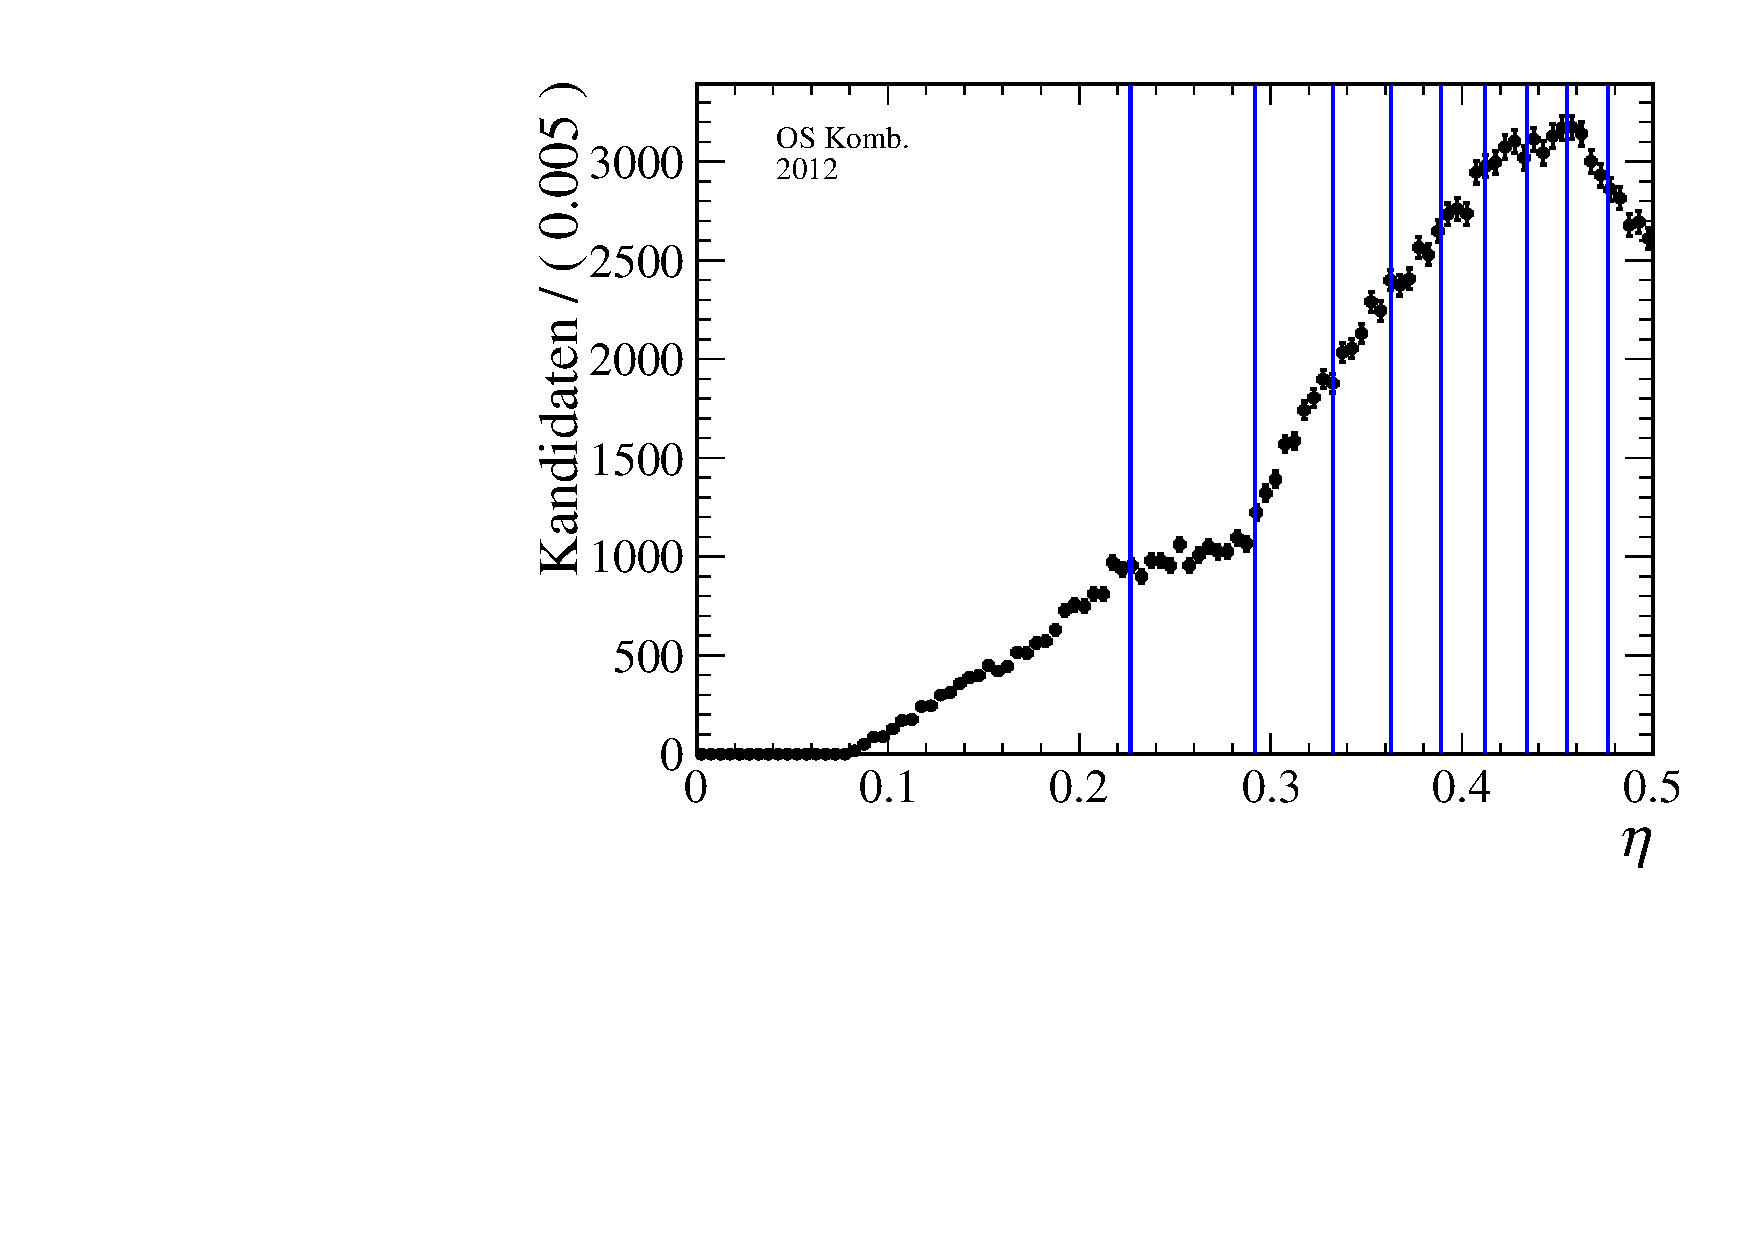
\includegraphics[width=0.75\textwidth]{fig/eta_trennung.pdf}
	\caption{Verteilung der mistag-Wahrscheinlichkeit $\eta$. Die senkrechten blauen Linien zeigen die Trennung in zehn Kategorien mit jeweils gleicher Statistik.}
	\label{fig:eta_trennung} 
\end{figure}
Der zugehörige lineare Fit an die $(\eta,\omega)$-Paare für das Jahr \num{2012} ist in Abbildung \ref{fig:2012_OScomb} zu sehen, die Ergebnisse in Tabelle \ref{tab:result_OScomb}.
\begin{figure}[htbp]
	\centering
		\includegraphics[width=0.75\textwidth]{fig/2012_OScomb.pdf}
	\caption{Fit des linearen Zusammenhangs an die $(\eta,\omega)$-Paare für die Standard OS Kombination auf Daten des Jahres \num{2012}}
	\label{fig:2012_OScomb} 
\end{figure}
\begin{table}[htbp]
	\centering
	\caption{Ergebnisse der Kalibrierung des OS Kombination für die Jahre \num{2011} und \num{2012}}
	\label{tab:result_OScomb}
	\begin{tabular}{ccccc}
	\toprule
       Jahr & $\langle\eta\rangle$ & $p_0$ & $\left|p_0-\langle\eta\rangle\right|$ & $p_1$ \\ 
       \midrule 
       2011 & $0{.}365$ & $0{.}369\pm0{.}003$ & $0{.}004$ & $0{.}952\pm0{.}032$ \\
      2012 & $0{.}370$ & $0{.}376\pm0{.}002$ & $0{.}006$ & $0{.}981\pm0{.}020$ \\ 
      \bottomrule
	\end{tabular}
\end{table} 
\begin{table}[htbp]
	\centering
	\caption{Performanz der Standard OS Kombination für das Jahr \num{2012}}
	\label{tab:2012_OScomb}
	\begin{tabular}{ccccc}
	\toprule
       Kategorie & $\varepsilon(\%)$ & $\omega$ & $D$ & $\varepsilon D^2(\%)$ \\ 
       \midrule
       1 & $3{,}865\pm0{,}035$ & $0{,}186\pm0{,}006$ & $0{,}628\pm0{,}012$ & $1{,}524\pm0{,}060$\\
       2 & $3{,}862\pm0{,}035$ & $0{,}262\pm0{,}006$ & $0{,}476\pm0{,}012$ & $0{,}875\pm0{,}045$\\ 
       3 & $3{,}832\pm0{,}035$ & $0{,}327\pm0{,}006$ & $0{,}346\pm0{,}012$ & $0{,}459\pm0{,}032$\\ 
       4 & $3{,}837\pm0{,}035$ & $0{,}360\pm0{,}006$ & $0{,}280\pm0{,}012$ & $0{,}301\pm0{,}026$\\ 
       5 & $3{,}810\pm0{,}035$ & $0{,}393\pm0{,}006$ & $0{,}214\pm0{,}012$ & $0{,}174\pm0{,}020$\\ 
       6 & $3{,}841\pm0{,}035$ & $0{,}411\pm0{,}006$ & $0{,}178\pm0{,}012$ & $0{,}122\pm0{,}016$\\ 
       7 & $3{,}842\pm0{,}035$ & $0{,}428\pm0{,}006$ & $0{,}144\pm0{,}012$ & $0{,}080\pm0{,}013$\\ 
       8 & $3{,}826\pm0{,}035$ & $0{,}449\pm0{,}006$ & $0{,}102\pm0{,}012$ & $0{,}040\pm0{,}009$\\ 
       9 & $3{,}823\pm0{,}035$ & $0{,}464\pm0{,}006$ & $0{,}072\pm0{,}012$ & $0{,}020\pm0{,}007$\\ 
      10 & $3{,}828\pm0{,}035$ & $0{,}486\pm0{,}006$ & $0{,}028\pm0{,}012$ & $0{,}003\pm0{,}003$\\ 
      \midrule
   Total & $38{,}366\pm0{,}112$& $0{,}377\pm0{,}002$ & $0{,}247\pm0{,}004$ & $3{,}597\pm0{,}091$\\ 
   \bottomrule
	\end{tabular}
\end{table}
Man erkennt zunächst, dass der Parameter $p_0$ um \num{3} Standardabweichungen von dem erwarteten $\langle\eta\rangle$ abweicht, der Parameter $p_1$ stimmt im Rahmen seiner Ungenauigkeit gut mit eins überein. Allerdings bestätigen die Datenpunkte die Annahme eines linearen Zusammenhangs zwischen der mistag-Wahrscheinlichkeit $\eta$ und dem true-mistag $\omega$. 
\begin{figure}[htbp]
	\centering
		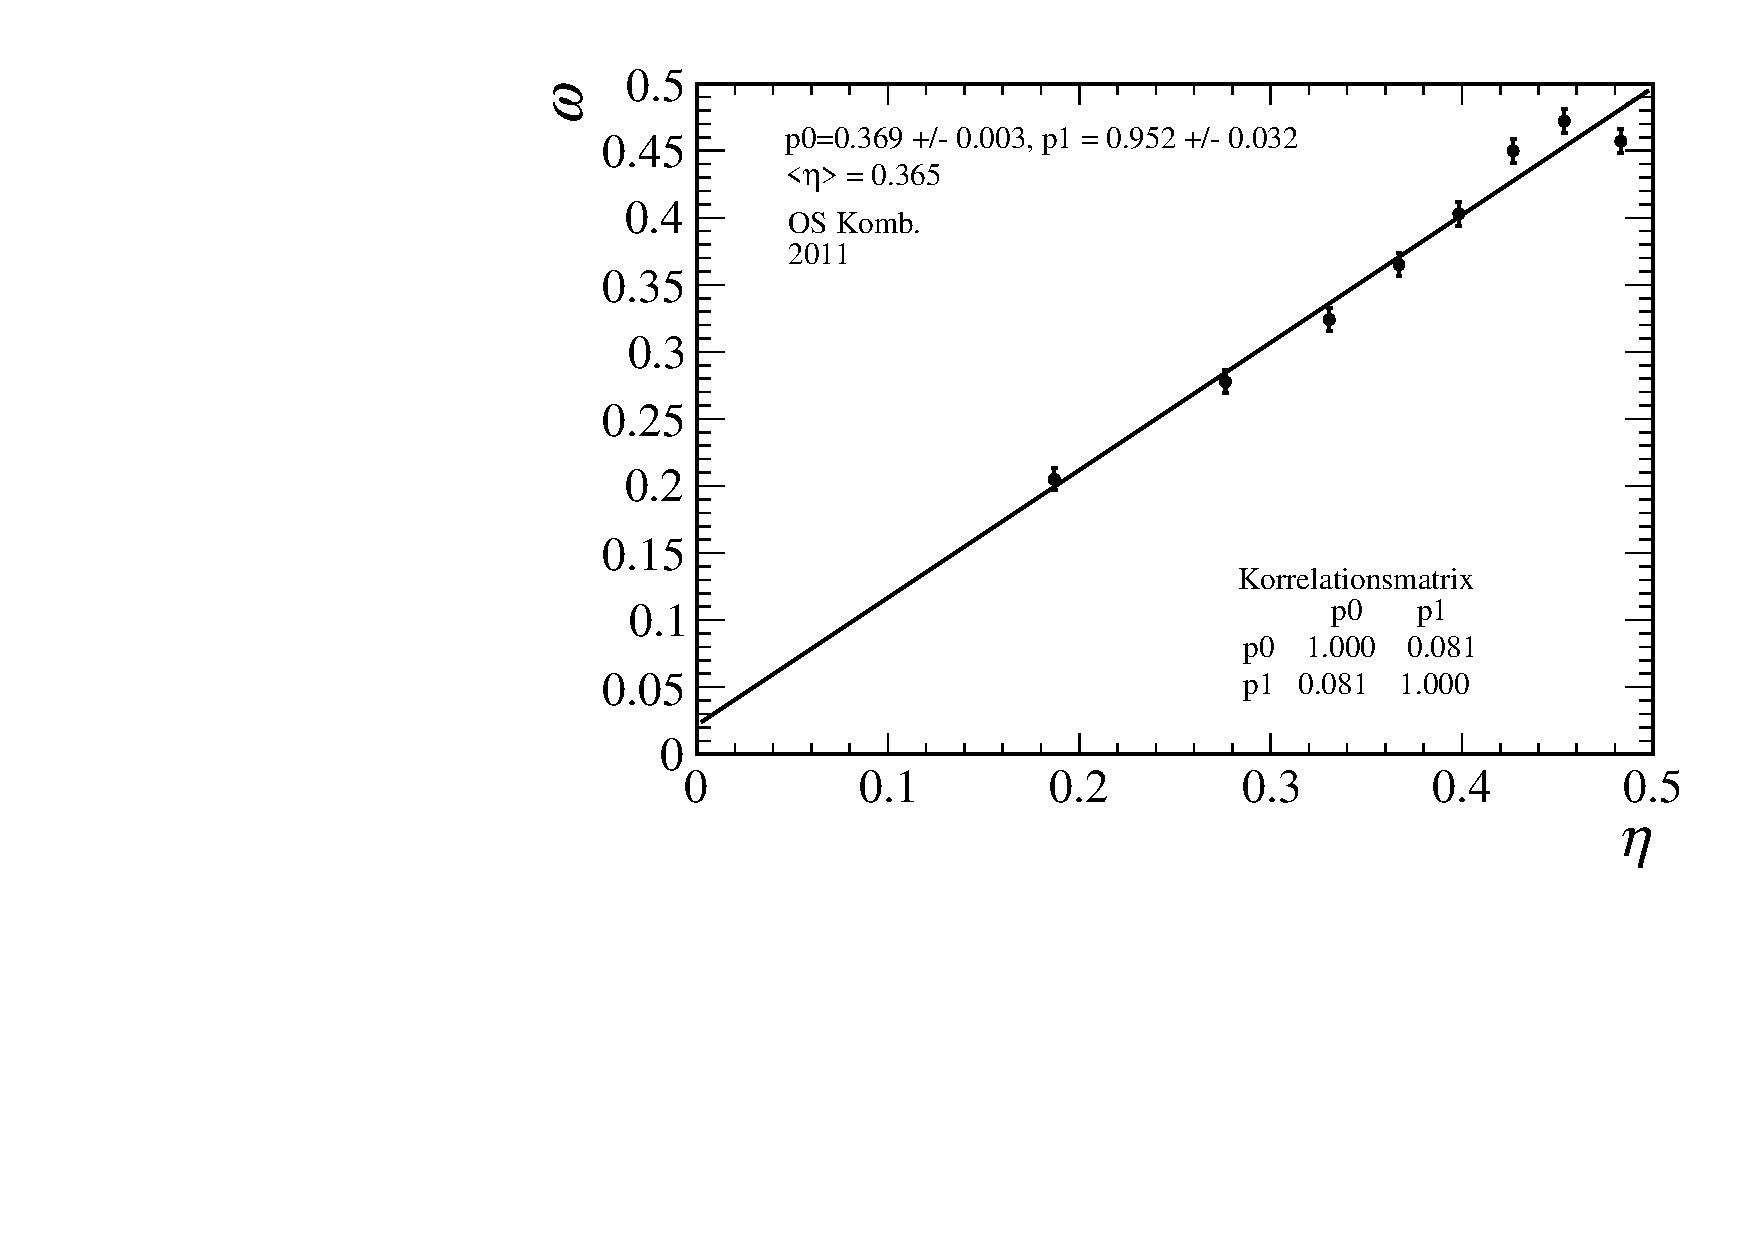
\includegraphics[width=0.75\textwidth]{fig/2011_OScomb.pdf}
	\caption{Fit des linearen Zusammenhangs an die $(\eta,\omega)$-Paare für die Standard OS Kombination auf Daten des Jahres \num{2011}}
	\label{fig:2011_OScomb} 
\end{figure} 
\begin{table}[htbp]
	\centering
	\caption{Performanz der Standard OS Kombination für das Jahr \num{2011}}
	\label{tab:2011_OScomb}
	\begin{tabular}{ccccc}
	\toprule
       Kategorie & $\varepsilon(\%)$ & $\omega$ & $D$ & $\varepsilon D^2(\%)$ \\ 
       \midrule 
       1 & $4{,}739\pm0{,}291$ & $0{,}205\pm0{,}008$ & $0{,}590\pm0{,}016$ & $1{,}650\pm0{,}135$\\
       2 & $4{,}723\pm0{,}290$ & $0{,}277\pm0{,}008$ & $0{,}446\pm0{,}016$ & $0{,}939\pm0{,}089$\\ 
       3 & $4{,}652\pm0{,}286$ & $0{,}324\pm0{,}008$ & $0{,}352\pm0{,}016$ & $0{,}576\pm0{,}063$\\ 
       4 & $4{,}664\pm0{,}287$ & $0{,}365\pm0{,}008$ & $0{,}270\pm0{,}016$ & $0{,}340\pm0{,}045$\\ 
       5 & $4{,}650\pm0{,}286$ & $0{,}403\pm0{,}008$ & $0{,}194\pm0{,}016$ & $0{,}175\pm0{,}031$\\ 
       6 & $4{,}673\pm0{,}287$ & $0{,}450\pm0{,}008$ & $0{,}100\pm0{,}016$ & $0{,}047\pm0{,}015$\\ 
       7 & $4{,}673\pm0{,}287$ & $0{,}472\pm0{,}008$ & $0{,}056\pm0{,}016$ & $0{,}015\pm0{,}008$\\ 
       8 & $4{,}675\pm0{,}288$ & $0{,}457\pm0{,}008$ & $0{,}086\pm0{,}016$ & $0{,}035\pm0{,}013$\\ 
       \midrule
   Total & $37{,}449\pm0{,}814$& $0{,}369\pm0{,}003$ & $0{,}262\pm0{,}006$ & $3{,}777\pm0{,}183$\\ 
   \bottomrule
	\end{tabular}
\end{table}
Die Ergebnisse des Jahres \num{2011} sind in der Abbildung \ref{fig:2011_OScomb}  und in der Tabelle \ref{tab:result_OScomb} zu sehen. Hier stimmen beide Parameter im Fit zufriedenstellend mit ihren Erwartungen überein. Ebenso ist der lineare Zusammenhang in den Datenpunkten gut erkennbar.\\
Die Ergebnisse für die Taggingeffizienzen $\varepsilon$ und effektiven Taggingeffizienzen $\varepsilon D^2$ für beide Jahre sind in den Tabellen \ref{tab:2012_OScomb} und \ref{tab:2011_OScomb} zu sehen. Dabei sieht man hier jeweils die Einzelergebnisse für die verschiedenen Kategorien der mistag-Wahrscheinlichkeit $\eta$. Man beobachtet, dass, obwohl alle Kategorien eine nahezu identische Statistik beitragen, die ersten Kategorien, aufgrund ihrer kleinen Werte für $\omega$ am stärksten zu effektiven Taggingeffizienz $\epsilon D^2$ beitragen. Die höheren Kategorien tragen mit größer werdenden true-mistag-Wahrscheinlichkeiten dann immer weniger zur gesamten effektiven Taggingeffizienz $\varepsilon D^2$ bei. Insgesamt sind die Ergebnisse der Taggingeffizienzen für beide Jahre vergleichbar und die Tagger können als kalibriert angesehen werden. Die Abweichung für das Jahr \num{2012} resultiert dabei aus der Tatsache, dass die Kalibrierung an dieser Stelle aus dem Zerfallskanal \BuToJPsiKp stammt und daher experimentell durchaus Unterschiede in den Kalibrierungsparametern $p_0$ und $p_1$ zu erwarten sind. Weiter sind an dieser Stelle noch keine systematischen Unsicherheiten berücksichtigt. 

\subsection{Der OS Charm Tagger}

Für den OS Charm Tagger erhält man im Jahr \num{2011} eine Taggingeffizienz von $\varepsilon=\SI{3{,}264}{\%}$ und für das Jahr \num{2012} von $\varepsilon=\SI{3{,}304}{\%}$ . Aufgrund der in beiden Jahren relativ geringen Statistik wurde eine minimale Anzahl von fünf Kategorien gewählt, um eine vertretbare Anzahl Datenpunkte für den linearen Fit zu behalten. Die Ergebnisse der linearen Fits sind in Abbildung \ref{fig:fit_OSCharm} und in Tabelle \ref{tab:result_OSCharm} zu sehen.
\begin{figure}[htbp]
	\centering
		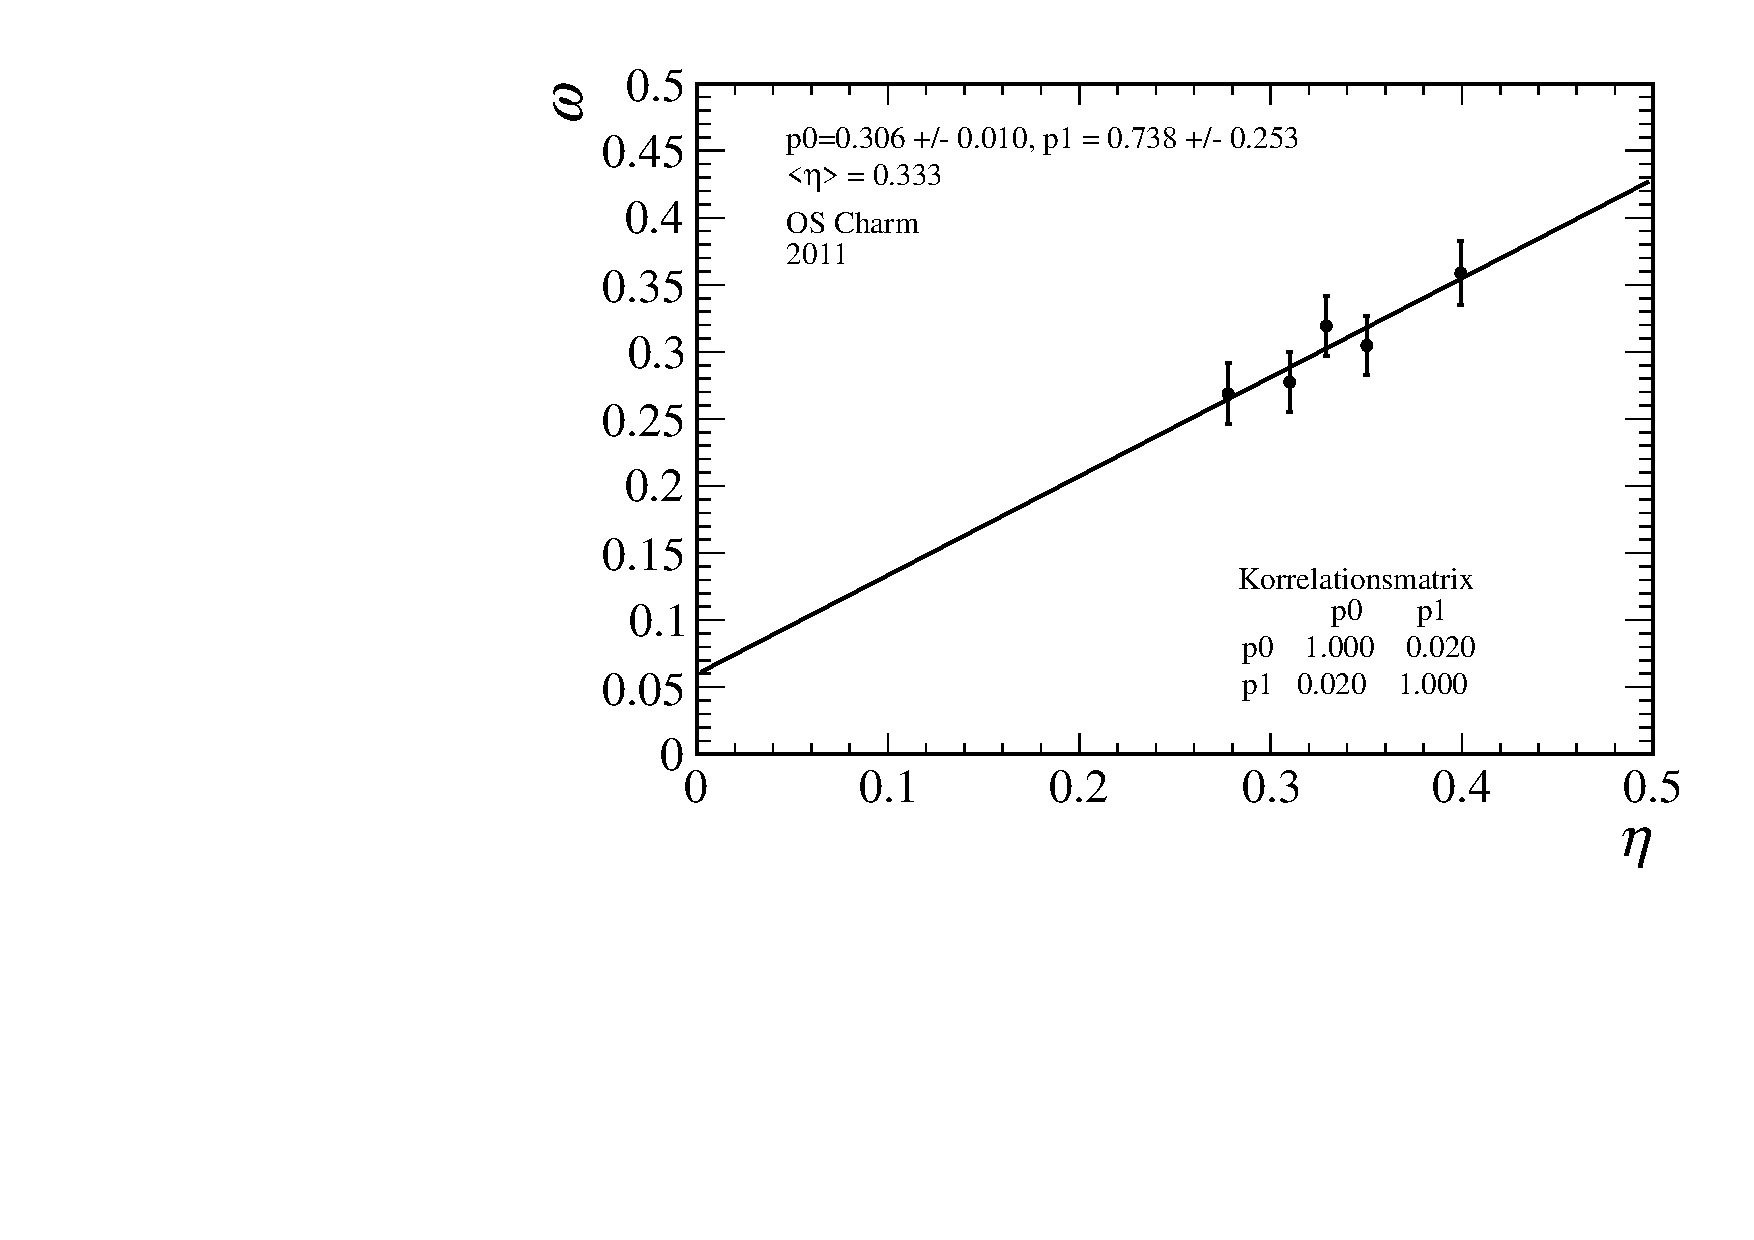
\includegraphics[width=0.49\textwidth]{fig/2011_OSCharm.pdf}
		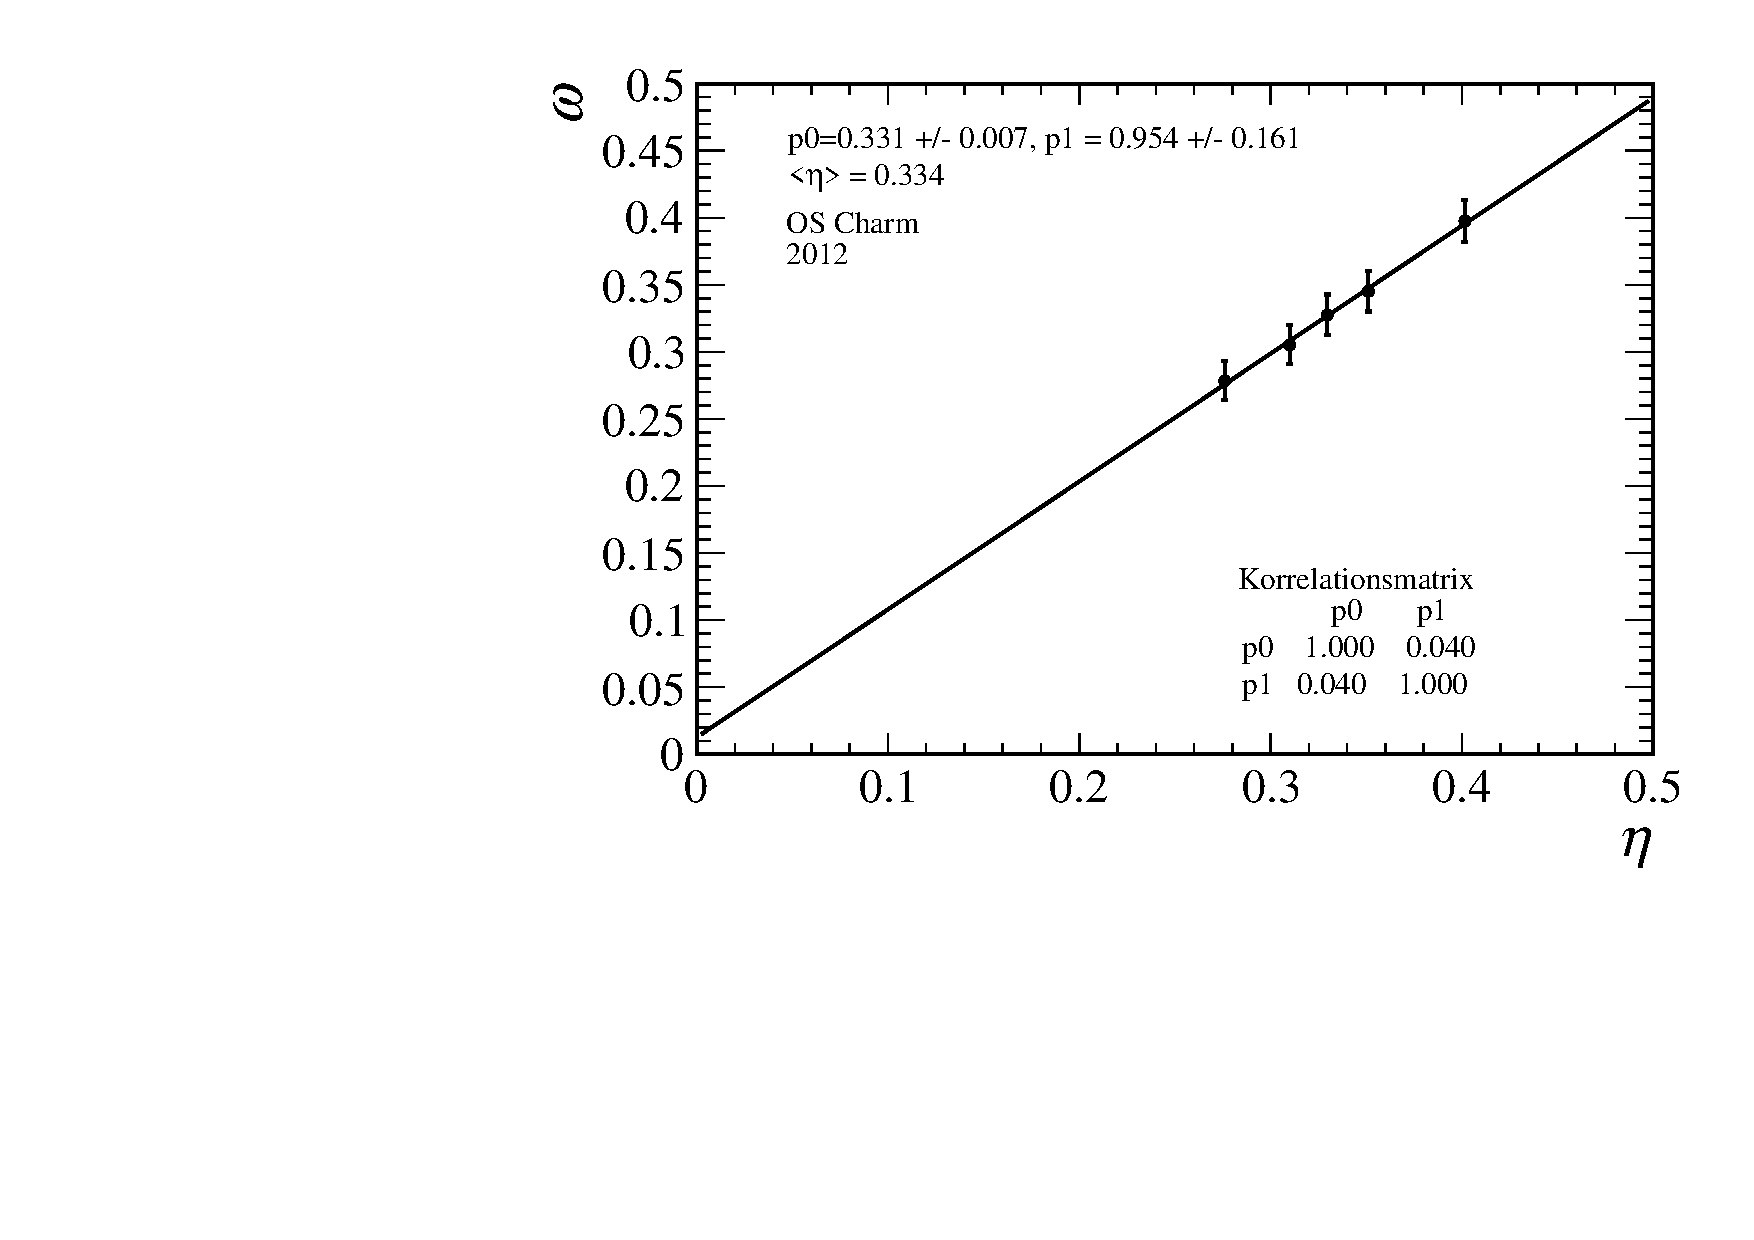
\includegraphics[width=0.49\textwidth]{fig/2012_OSCharm.pdf}
	\caption{Fit des linearen Zusammenhangs an die $(\eta,\omega)$-Paare für den OS Charm Tagger auf Daten des Jahres \num{2011} (links) und \num{2012} (rechts).}
	\label{fig:fit_OSCharm} 
\end{figure} 
Für das Jahr \num{2012} liegen beide Parameter des linearen Fits innerhalb einer Standardabweichung in ihren Erwartungen und die Datenpunkte sind sehr linear, sodass der Tagger hier als kalibiert angesehen werden kann. 
\begin{table}[htbp]
	\centering
	\caption{Ergebnisse der Kalibrierung des OS Charm Taggers für die Jahre \num{2011} und \num{2012}}
	\label{tab:result_OSCharm}
	\begin{tabular}{ccccc}
	\toprule
       Jahr & $\langle\eta\rangle$ & $p_0$ & $\left|p_0-\langle\eta\rangle\right|$ & $p_1$ \\ 
       \midrule
       2011 & $0{.}333$ & $0{.}306\pm0{.}010$ & $0{.}027$ & $0{.}738\pm0{.}253$ \\
      2012 & $0{.}334$ & $0{.}331\pm0{.}007$ & $0{.}003$ & $0{.}954\pm0{.}161$ \\ 
      \bottomrule
	\end{tabular}
\end{table}
\begin{table}[htbp]
	\centering
	\caption{Performanz des OS Charm Taggers für die Jahre \num{2011} und \num{2012}.}
	\label{tab:performance_OSCharm}
	\begin{tabular}{ccccc}
	\toprule
       Jahr & $\varepsilon(\%)$ & $\omega$ & $D$ & $\varepsilon D^2(\%)$ \\ 
       \midrule
      2011 & $3{,}304\pm0{,}102$ & $0{,}306\pm0{,}010$ & $0{,}388\pm0{,}020$ & $0{,}512\pm0{,}049$\\ 
   2012 & $3{,}264\pm0{,}032$ & $0{,}331\pm0{,}007$ & $0{,}338\pm0{,}014$ & $0{,}395\pm0{,}041$\\ 
   \bottomrule
  \end{tabular}
\end{table}
Die Ergebnisse für das Jahr \num{2011} zeigen eine etwas schlechtere Linearität der $(\eta,\omega)$-Paare, außerdem weicht der Parameter $p_0$ um \num{2{,}7} Standardabweichungen von dem erwarteten $\langle\eta\rangle$ ab.\\
Die Taggingeffizienzen $\varepsilon$ und die effektiven Taggingeffizienzen $\varepsilon D^2$  (Tabelle \ref{tab:performance_OSCharm}) sind für das Jahr \num{2011} in beiden Jahren etwas höher. Insgesamt können auch hier beide Tagger als kalibriert angesehen werden, die Abweichung für den Parameter $p_0$ für das Jahr \num{2011} resultieren dabei wieder aus einer Kalibrierung in einem anderen Zerfallskanal.\\
Weiterhin wird hier bestätigt, dass der OS Charm Tagger eine geringe Anzahl an getaggten Ereignisse aufweist, jedoch ebenso kleine mistag-Vorhersagen $\omega$ ausgibt. Somit ergibt sich, vor allem wegen der sehr kleinen Taggingeffizienzen $\varepsilon$, eine kleine effektive Taggingeffizienz $\varepsilon D^2$. 

\subsection{Der OS Kaon nnet Tagger}

Ebenso wie bei dem OS Charm Tagger handelt es sich bei dem OS Kaon nnet Tagger um eine Neuentwicklung. Allerdings liefert der OS Kaon nnet Tagger vergleichsweise große Anzahlen an getaggten Ereignissen mit großen mistag-Vorhersagen $\omega$. Für das Jahr \num{2011} erhält man in $\Bz\rightarrow\Dp\pim$ Taggingeffizienzen von $\varepsilon=\SI{45{,}044}{\%}$ und für das Jahr \num{2012} vom $\varepsilon=\SI{46{,}459}{\%}$. Da die mistag-Wahrscheinlichkeiten jedoch bei Werten $>\num{0{,}4}$ liegen (Abbildung \ref{fig:eta_oskaon}), werden trotz der hohen Ereigniszahlen weniger Kategorien als beispielsweise für die OS Standard Kombination gewählt. 
\begin{figure}[htbp]
	\centering
		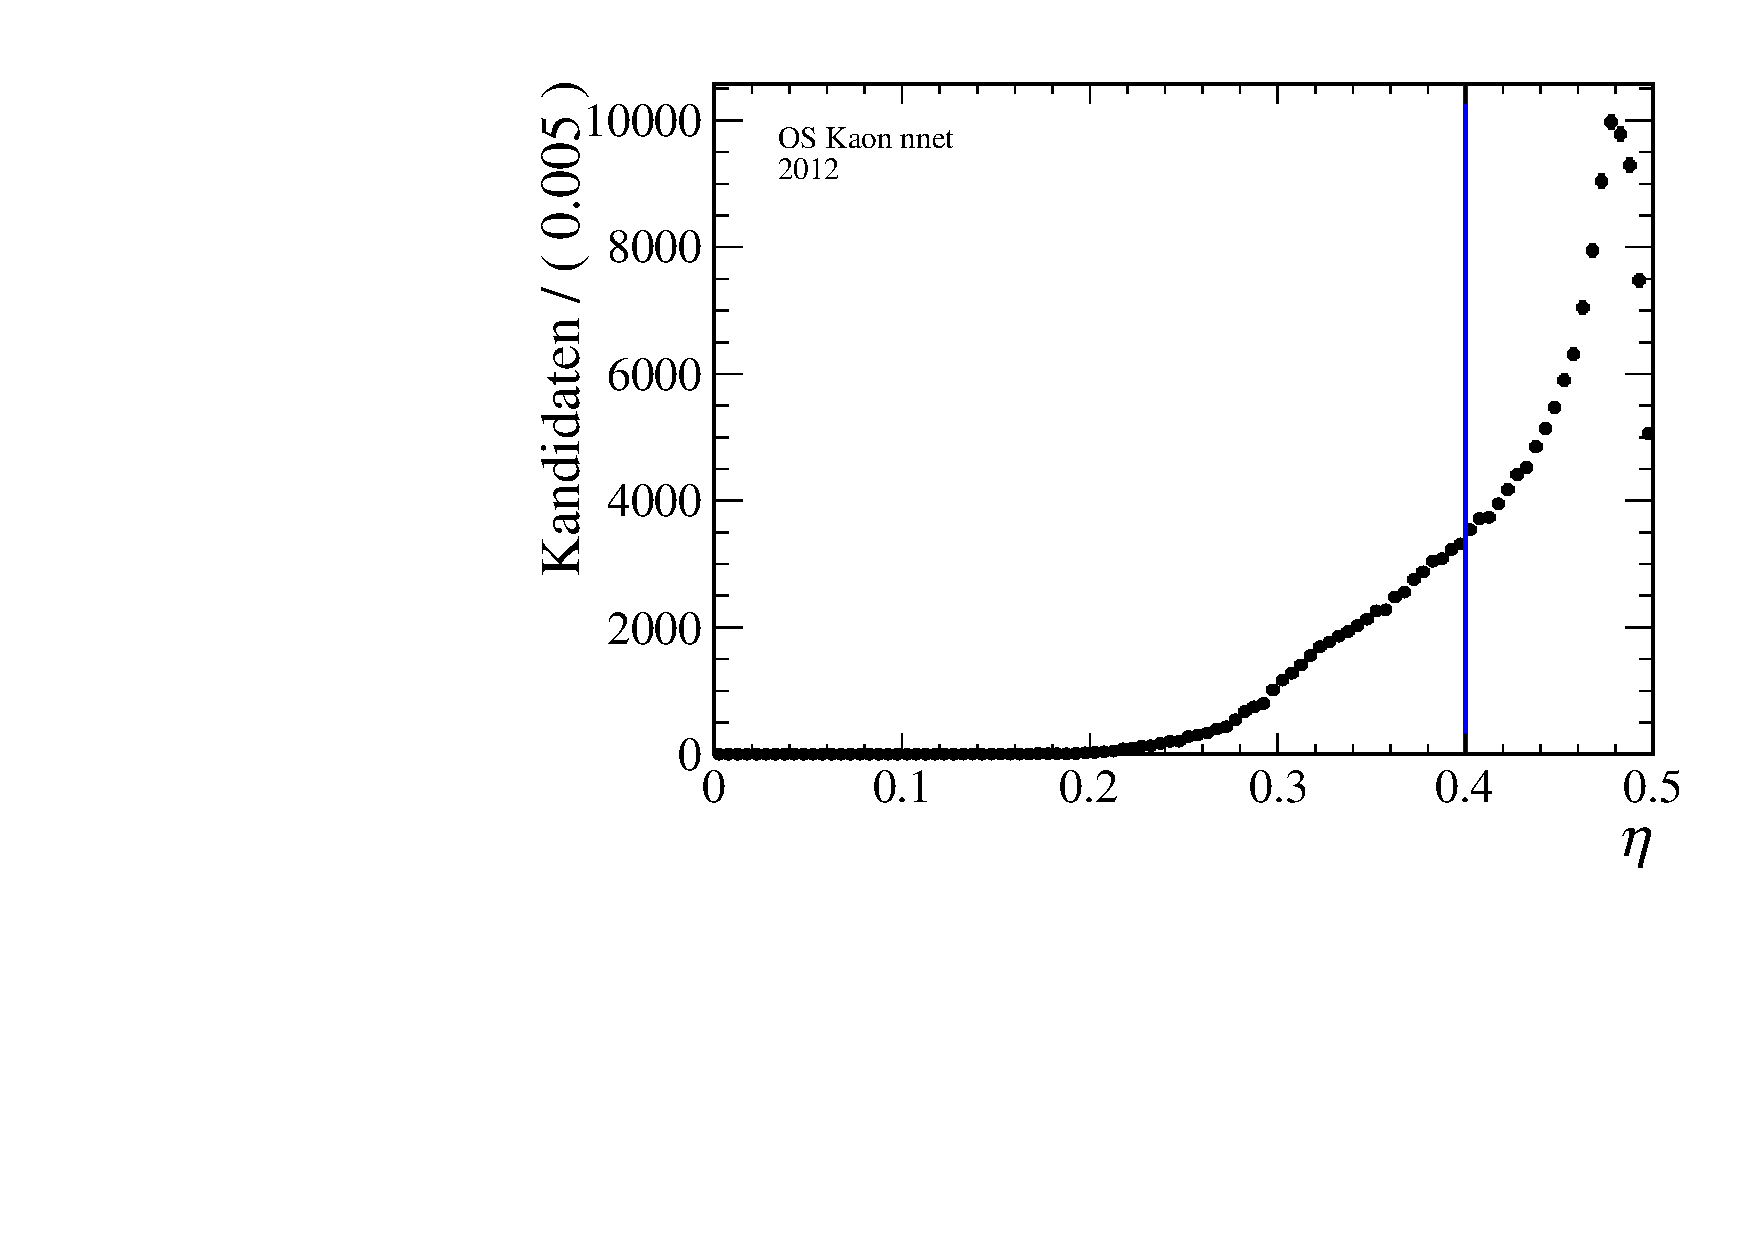
\includegraphics[width=0.75\textwidth]{fig/Eta_OSKaon.pdf}
	\caption{Verteilung der mistag-Wahrscheinlichkeit $\eta$ für den OS Kaon nnet Tagger für das Jahr \num{2012}. Man sieht, dass die meisten Kandidaten $\eta$-Werte über \num{0{,}4} (blaue senkrechte Linie) haben.}
	\label{fig:eta_oskaon} 
\end{figure} 
Die Ergebnisse der linearen Fits sind in Abbildung \ref{fig:fit_OSKaonNN} und Tabelle \ref{tab:result_OSKaonNN} zu sehen.
\begin{figure}[htbp]
	\centering
		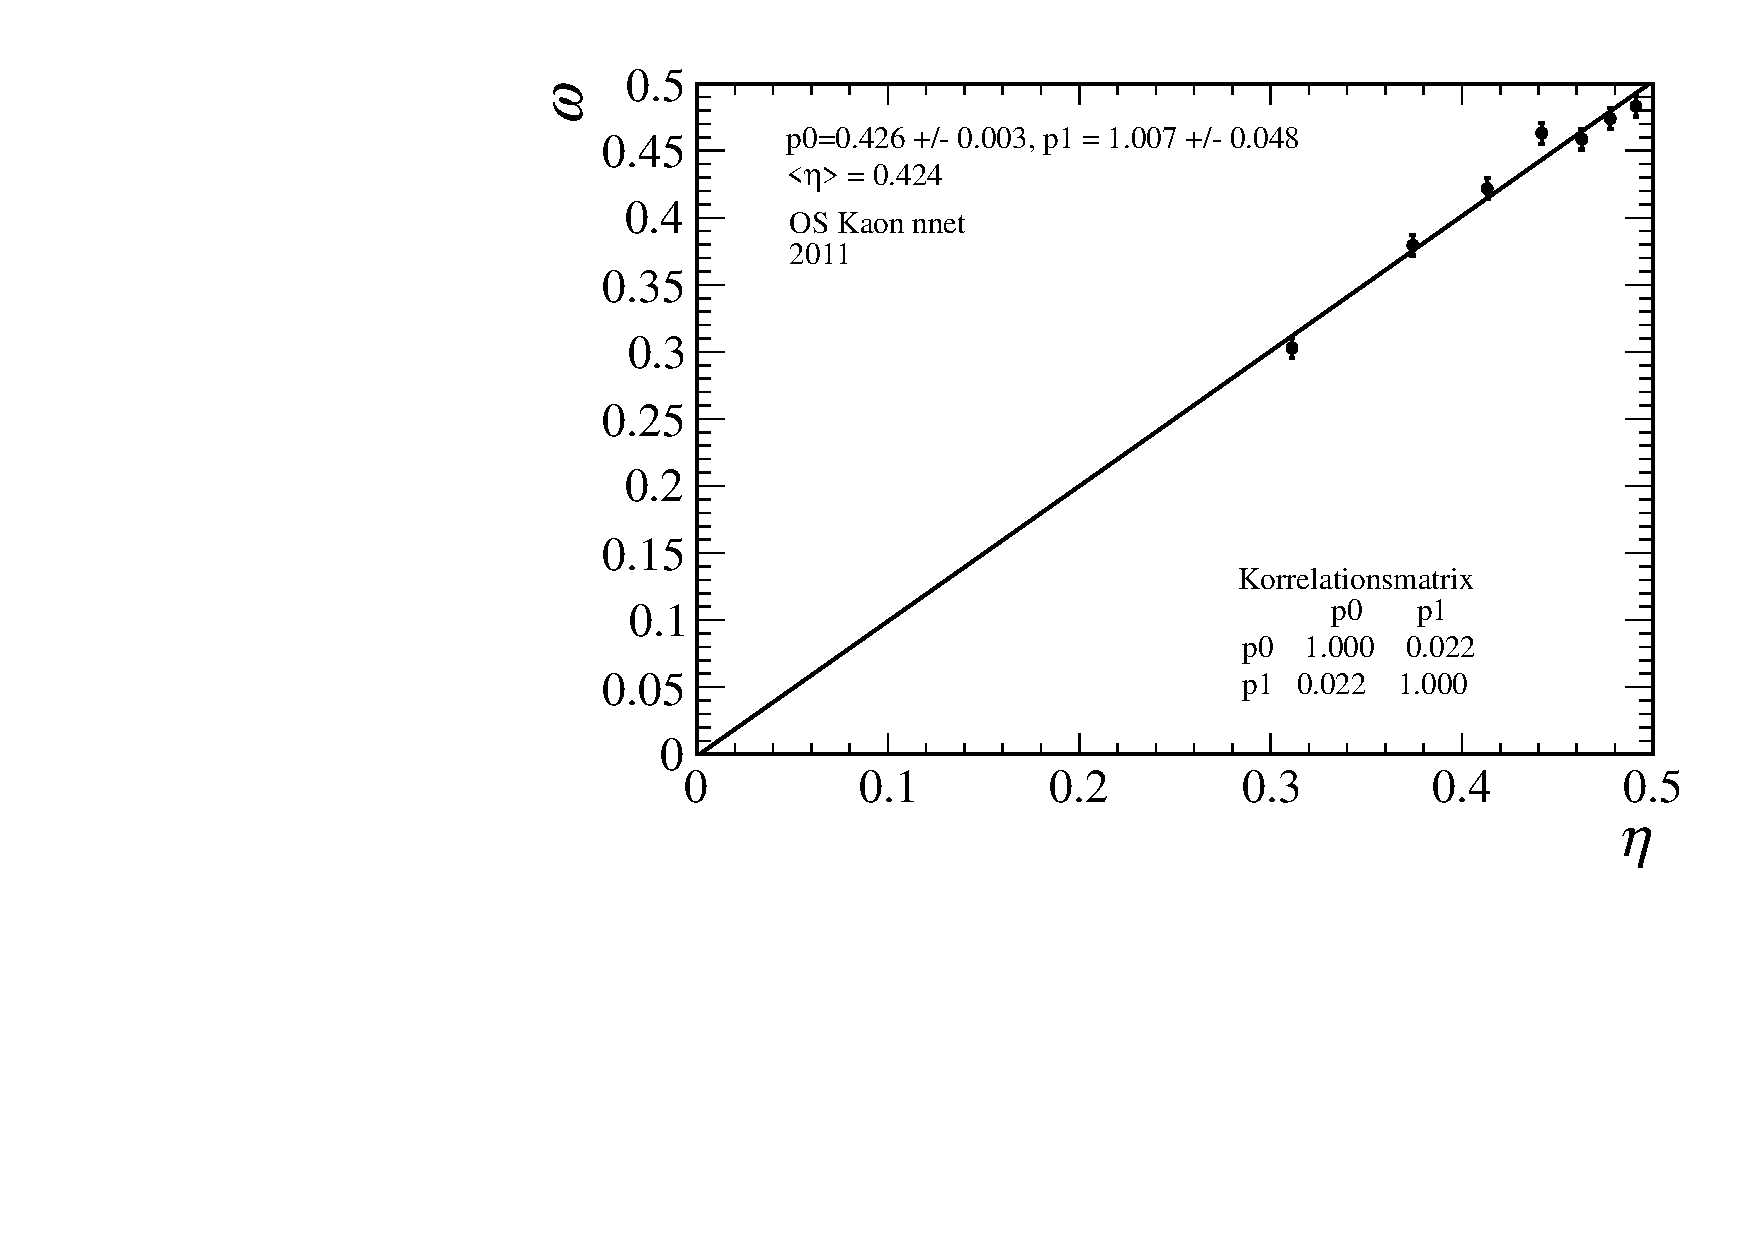
\includegraphics[width=0.49\textwidth]{fig/2011_OSKaonNN.pdf}
		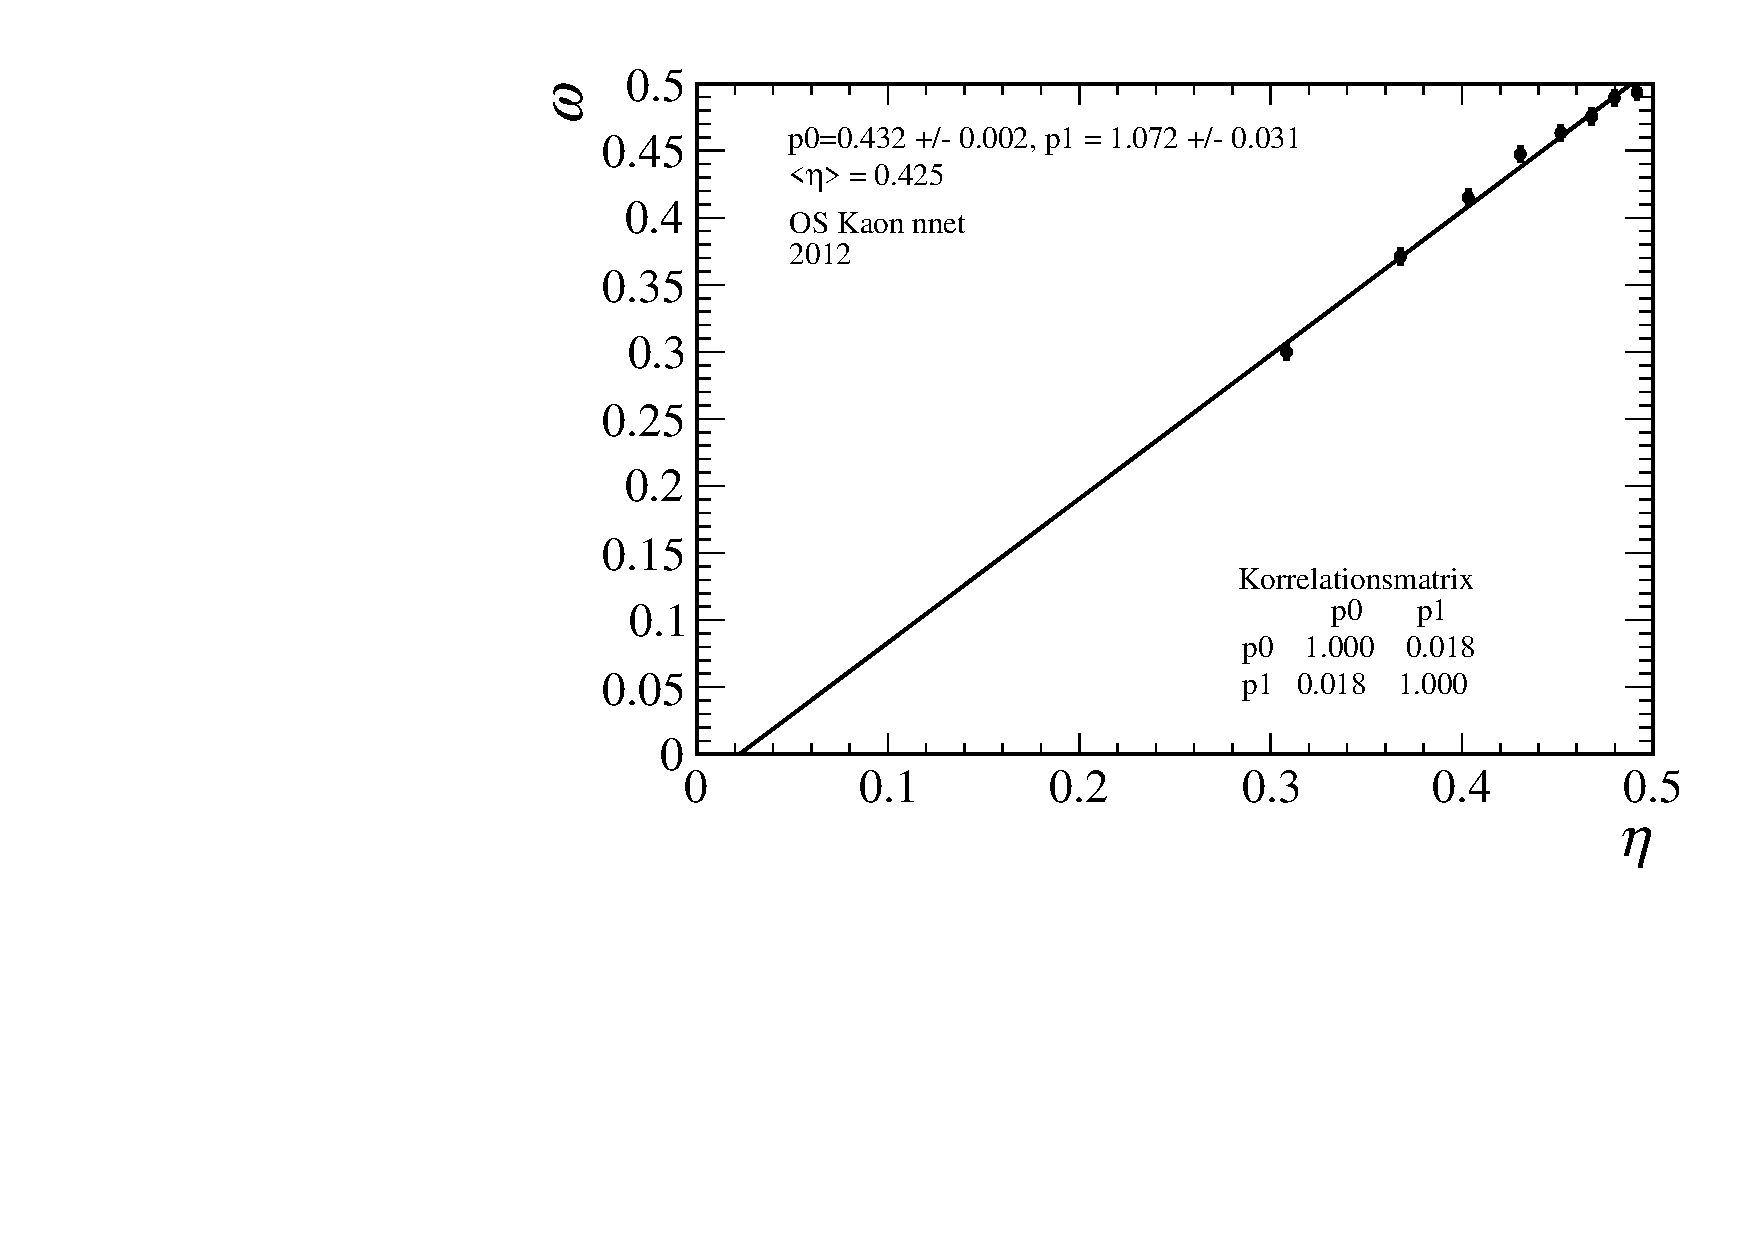
\includegraphics[width=0.49\textwidth]{fig/2012_OSKaonNN.pdf}
	\caption{Fit des linearen Zusammenhangs an die $(\eta,\omega)$-Paare für den OS Kaon nnet Tagger auf Daten des Jahres \num{2011} (links) und \num{2012} (rechts).}
	\label{fig:fit_OSKaonNN} 
\end{figure} 
Wie bei der Standard OS Kombination, ist auch hier zu sehen, dass die Kalibrierung für das Jahr \num{2012} nicht optimal ist. Beide Parameter $p_0$ und $p_1$ weichen um mehr als \num{2} Standardabweichungen von ihren Erwartungen ab. Allerdings wird auch hier der lineare Zusammenhang zwischen der vorhergesagten mistag-Wahrscheinlichkeit $\eta$ und dem true-mistag $\omega$ bestätigt. Für das Jahr \num{2011} stimmen beide Parameter gut mit ihren Erwartungen überein.  
\begin{table}[htbp]
	\centering
	\caption{Ergebnisse der Kalibrierung des OS Kaon nnet Taggers für die Jahre \num{2011} und \num{2012}.}
	\label{tab:result_OSKaonNN}
	\begin{tabular}{ccccc}
	\toprule
       Jahr & $\langle\eta\rangle$ & $p_0$ & $\left|p_0-\langle\eta\rangle\right|$ & $p_1$ \\ 
       \midrule 
	2011 & $0{.}425$ & $0{.}426\pm0{.}003$ & $0{.}001$ & $1{.}007\pm0{.}048$ \\
   2012 & $0{.}425$ & $0{.}432\pm0{.}002$ & $0{.}007$ & $1{.}073\pm0{.}031$ \\ 
   \bottomrule
	\end{tabular}
\end{table}
\begin{table}[htbp]
	\centering
	\caption{Performanz des OS Kaon nnet für die Jahre \num{2011} und \num{2012}.}
	\label{tab:performance_OSKaonNN}
	\begin{tabular}{ccccc}
	\toprule
       Jahr & $\varepsilon(\%)$ & $\omega$ & $D$ & $\varepsilon D^2(\%)$ \\ 
       \midrule
       2011 & $45{,}044\pm1{,}041$& $0{,}426\pm0{,}003$ & $0{,}147\pm0{,}006$ & $1{,}621\pm0{,}122$\\
     2012 & $46{,}459\pm0{,}125$& $0{,}432\pm0{,}002$ & $0{,}136\pm0{,}004$ & $1{,}588\pm0{,}061$\\ 
     \bottomrule
  \end{tabular}
\end{table}
Die in Tabelle \ref{tab:performance_OSKaonNN} dargestellten Taggingeffizienzen $\varepsilon$ sind für beide Jahre ähnlich, ebenso die effektiven Taggingeffizienz $\varepsilon D^2$. Zusammenfassend lässt sich der Tagger für das Jahr \num{2011} als gut kalibriert bezeichnen, für das Jahr \num{2012} ist diese Aussage schwieriger. Die größeren Abweichungen für das Jahr \num{2012} haben vermutlich die gleiche Ursache wie bei der Standard OS Kombination. Aus diesem Grund lässt sich für das Jahr \num{2012} sagen, dass der OS Kaon nnet Tagger kalibriert ist, diese Kalibration auf \BdToDpi allerdings nicht ideal ist.   

\section{Kalibrierung der SS Tagger}

Im Weiteren wird nun auf die Kalibrierung der SS Tagger eingegangen. Die Parameter der Zerfallszeitakzeptanz werden dabei ebenfalls wieder in allen Kanälen mit dem zuvor beschriebenen \sPlot-Verfahren \cite{splot} bestimmt. Da die gesuchten Taggingteilchen für die Tagger auf der Same Side dem Signal deutlich ähnlicher sind, wird bei ihrer Selektion das Signal mit beeinflusst. Dadurch kommt es in den unterschiedlichen Kategorien der mistag-Verteilung $\eta$ zu Unterschieden, die im Fit berücksichtigt werden müssen.

\subsection{Der SS Pion Tagger}

Der schnittbasierten SS Pion Tagger hat für das Jahr \num{2011} eine Taggingeffizienz von $\varepsilon=\SI{14{,}847}{\%}$ und für das Jahr \num{2012} von $\varepsilon=\SI{15{,}146}{\%}$. Für \num{2011} werden sechs und für \num{2012} sieben $\eta$-Kategorien gewählt. In Abbildung \ref{fig:fit_SSPion} und Tabelle \ref{tab:result_SSPion} sind die Ergebnisse der Kalibrierung für die Jahre \num{2011} und \num{2012} dargestellt.
\begin{figure}[htbp]
	\centering
		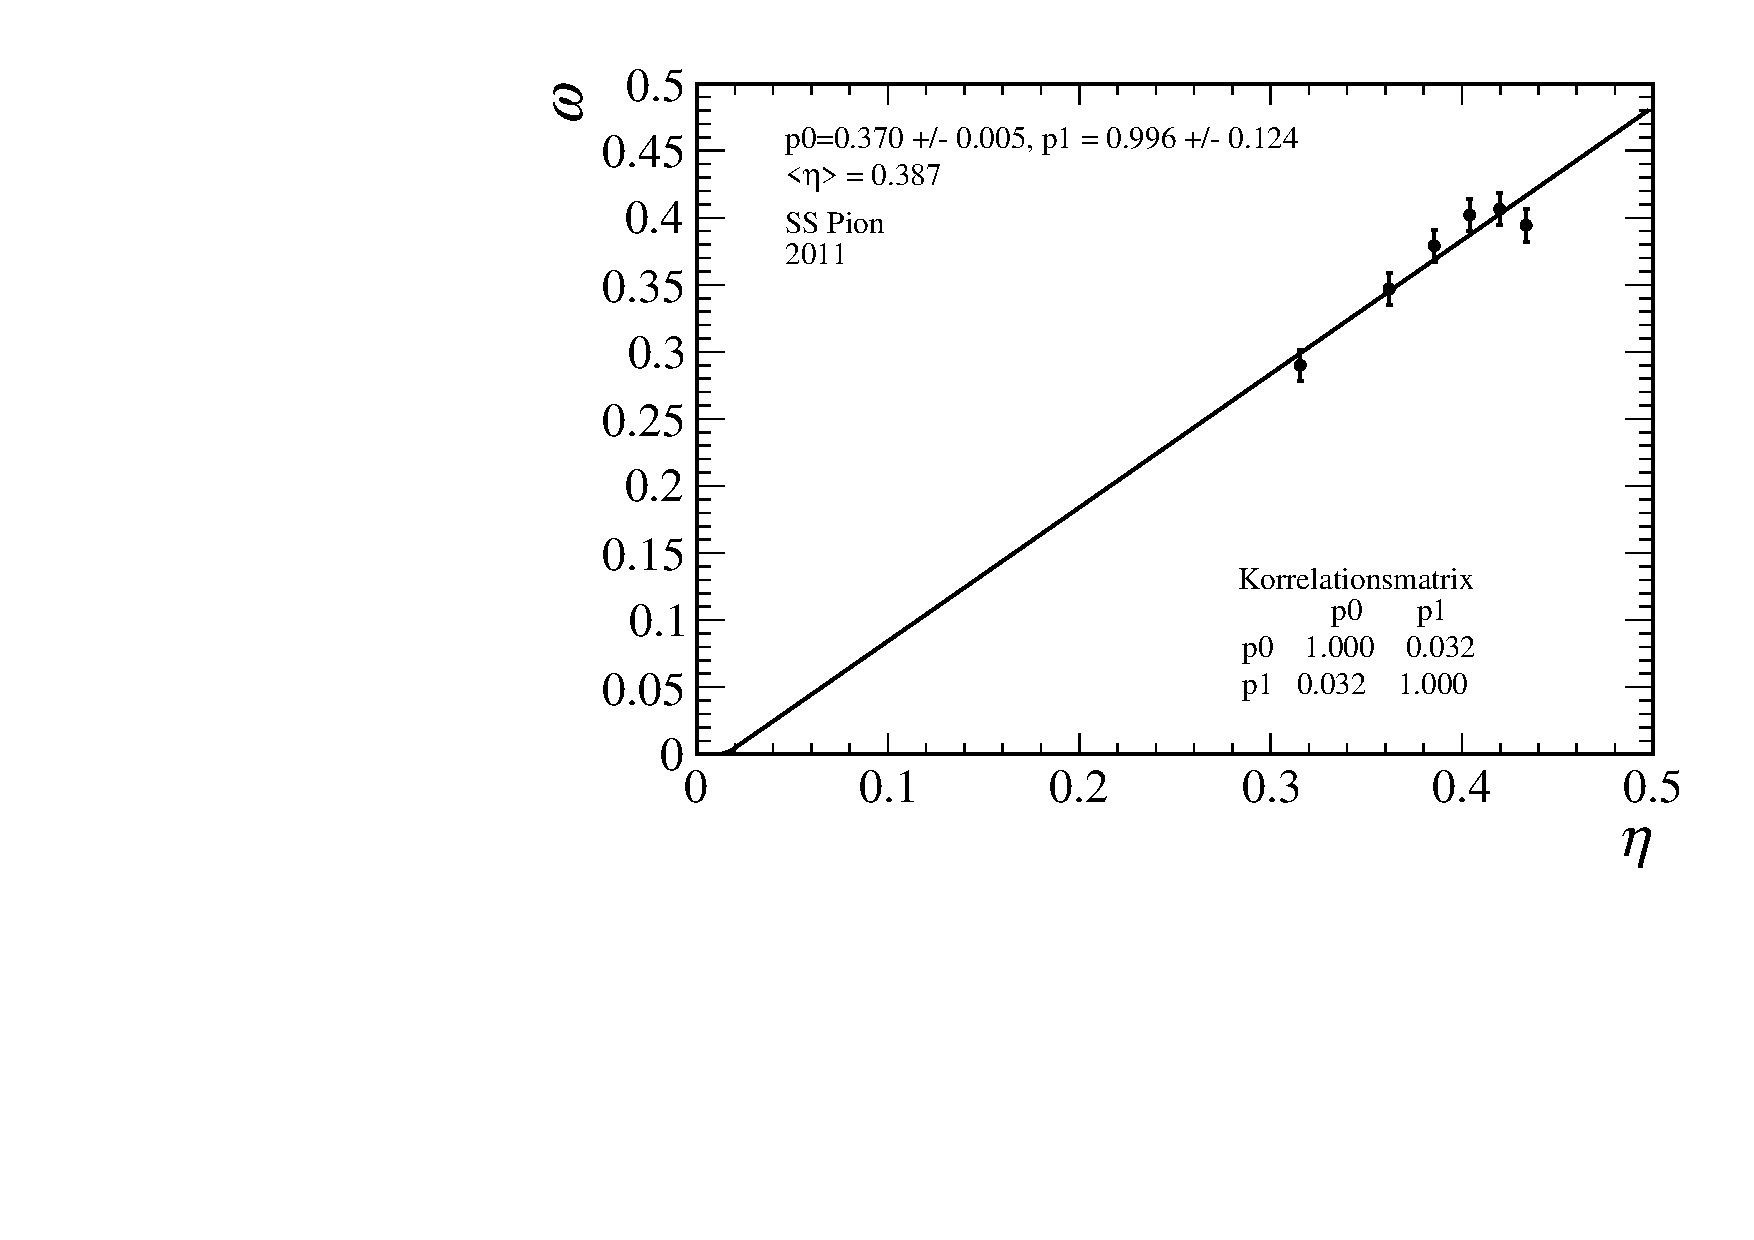
\includegraphics[width=0.49\textwidth]{fig/2011_SSPion.pdf}
		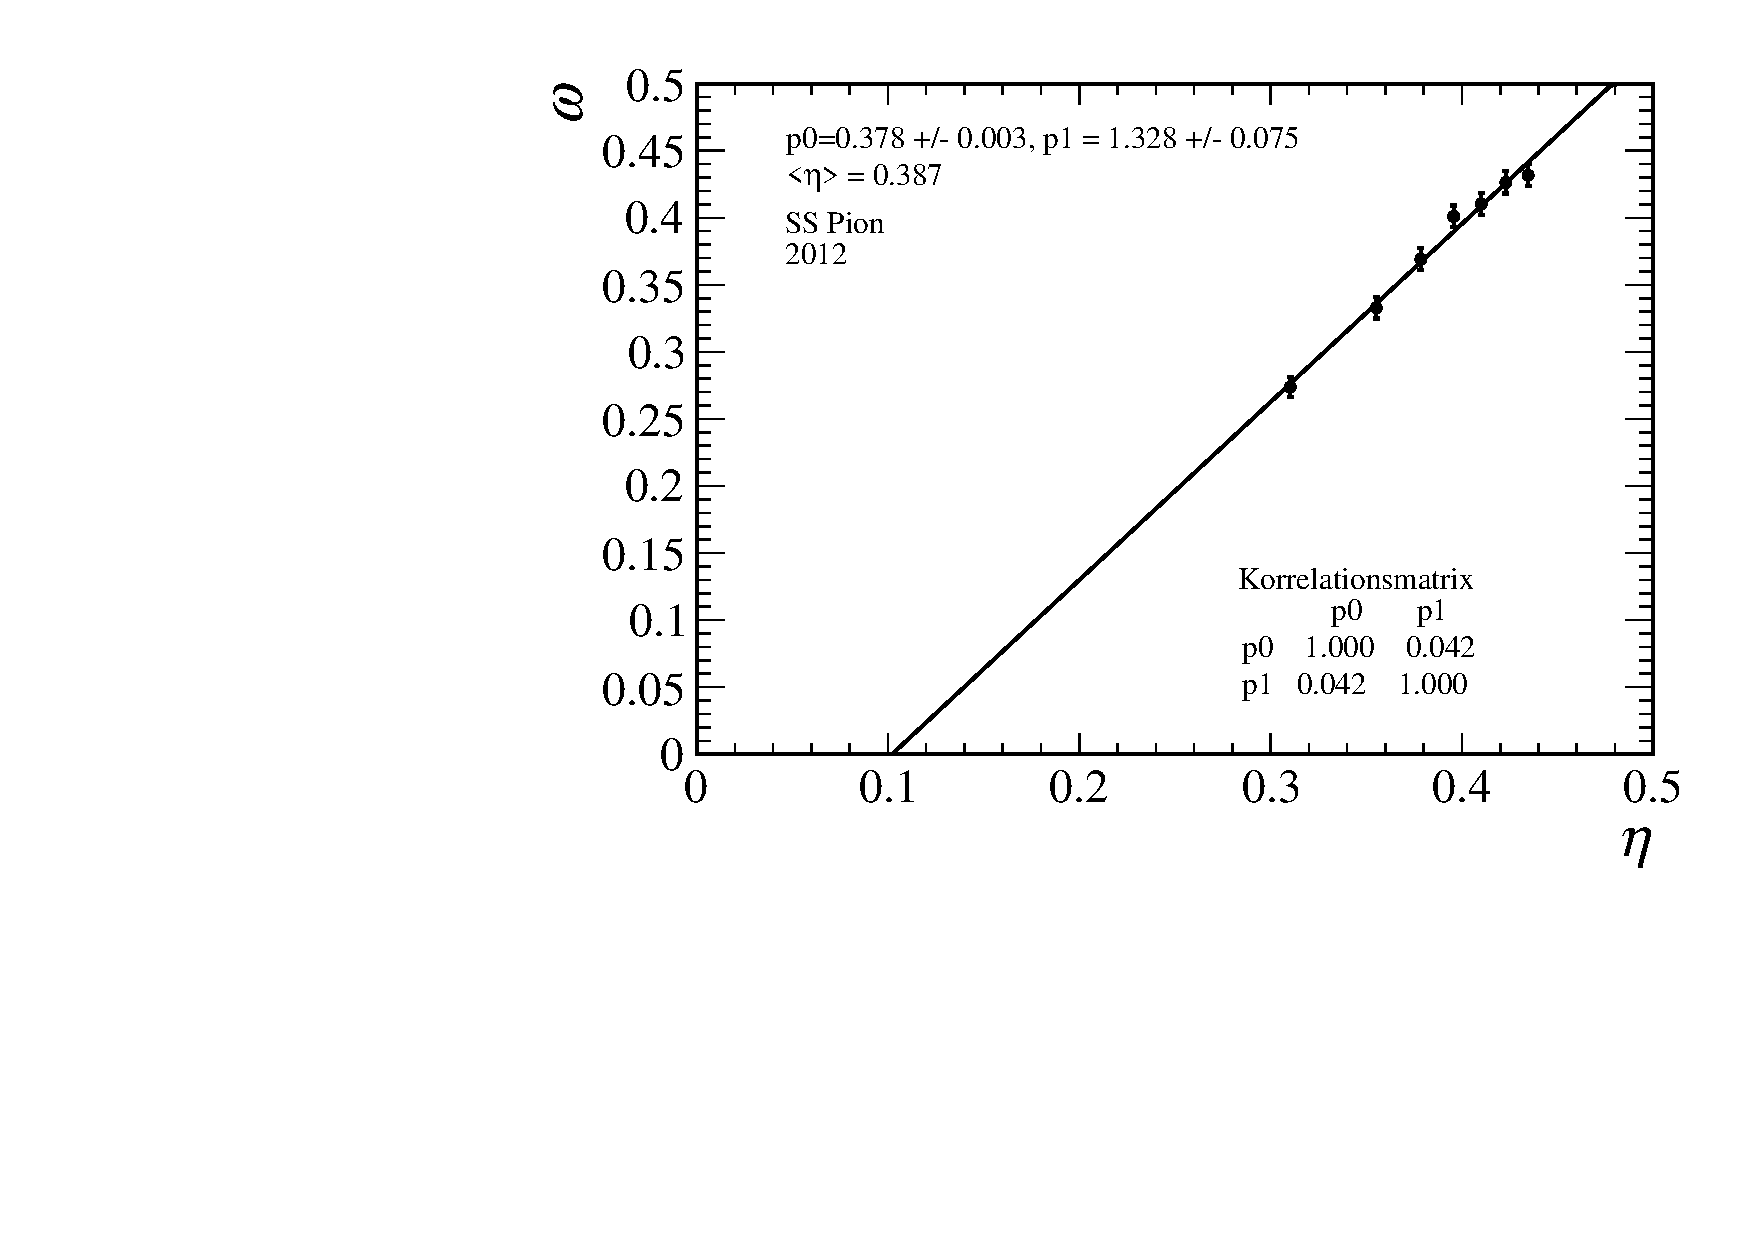
\includegraphics[width=0.49\textwidth]{fig/2012_SSPion.pdf}
	\caption{Fit des linearen Zusammenhangs an die $(\eta,\omega)$-Paare für den SS Pion Tagger auf Daten des Jahres \num{2011} (links) und \num{2012} (rechts).}
	\label{fig:fit_SSPion} 
\end{figure}
Für das Jahr \num{2012} wird deutlich, dass die Kalibrationsparameter $p_0$ und $p_1$ stark von den Erwartungen einer idealen Kaibrierung abweichen.
\begin{table}[htbp]
	\centering
	\caption{Ergebnisse der Kalibrierung des schnittbasierten SS Pion Taggers für die Jahre \num{2011} und \num{2012}.}
	\label{tab:result_SSPion}
	\begin{tabular}{ccccc}
	\toprule
       Jahr & $\langle\eta\rangle$ & $p_0$ & $\left|p_0-\langle\eta\rangle\right|$ & $p_1$ \\
       \midrule
	2011 & $0{.}387$ & $0{.}370\pm0{.}005$ & $0{.}017$ & $0{.}996\pm0{.}124$ \\
   2012 & $0{.}387$ & $0{.}378\pm0{.}003$ & $0{.}009$ & $1{.}328\pm0{.}075$ \\ 
   \bottomrule
	\end{tabular}
\end{table}
\begin{table}[htbp]
	\centering
	\caption{Performanz des schnittbasierten SS Pion Taggers für die Jahre \num{2011} und \num{2012}.}
	\label{tab:performance_SSPion}
	\begin{tabular}{ccccc}
	\toprule
       Jahr & $\varepsilon(\%)$ & $\omega$ & $D$ & $\varepsilon D^2(\%)$ \\ 
       \midrule
   2011 & $14{,}847\pm1{,}380$& $0{,}370\pm0{,}005$ & $0{,}261\pm0{,}010$ & $1{,}104\pm0{,}074$\\ 
   2012 & $15{.}146\pm0{.}070$ & $0{.}378\pm0{.}003$ & $0{.}244\pm0{.}006$ & $1{.}071\pm0{.}049$\\ 
   \bottomrule
	\end{tabular}
\end{table}
Bei der Kalibrierung für die Daten des Jahres \num{2011} weicht nur der Parameter $p_0$ stark ab, während $p_1$ innerhalb seines Fehlers kompatibel mit der Erwartung ist. \\
Betrachtet man die Taggingeffizienzen $\varepsilon$ und die effektiven Taggingeffizienzen $\varepsilon D^2$ (Tabelle \ref{tab:performance_SSPion}), so erkennt man, dass diese für beide Jahre vergleichbar sind. Für das Jahr \num{2011} lässt sich der Tagger als kalibriert ansehen. Für \num{2012}  zeigen die beobachtbaren Abweichungen beider Kalibrierungsparameter die in der Flavour-Tagging-Software vorgenommen Präkalibrierung jedoch als nicht ideal.  

\subsection{Der SS Pion BDT Tagger}

Der SS Pion BDT Tagger ist ebenfalls eine Neuentwicklung und soll zukünftig den schnittbasierten SS Pion Tagger ablösen. Er hat wie der OS Kaon nnet Tagger sehr viele getaggte Ereignisse mit tendenziell großen mistag-Wahrscheinlichkeiten $\eta$. Für das Jahr \num{2011} erhält man eine Taggingeffizienz von $\varepsilon=\SI{56{,}797}{\%}$ und für das Jahr \num{2012} von $\varepsilon=\SI{58{,}147}{\%}$. Die Ergebnisse der Kalibrierung sind in Abbildung \ref{fig:fit_SSPionBDT} und Tabelle \ref{tab:result_SSPionBDT} zu sehen. Da im Jahr \num{2012} die meisten $(\eta,\omega)$-Paare bei hohen mistag-Wahrscheinlichkeiten $\eta$ eng beieinander liegen, nutzt eine größere Anzahl an Kategorien hier nur wenig, weshalb die gleichen Anzahlen wie beim OS Kaon nnet Tagger genutzt wurden.  Die Kalibrierungsparameter weichen beide um mehr als zwei Standardabweichungen von ihren perfekt kalibrierten Werten ab. 
\begin{figure}[htbp]
	\centering
		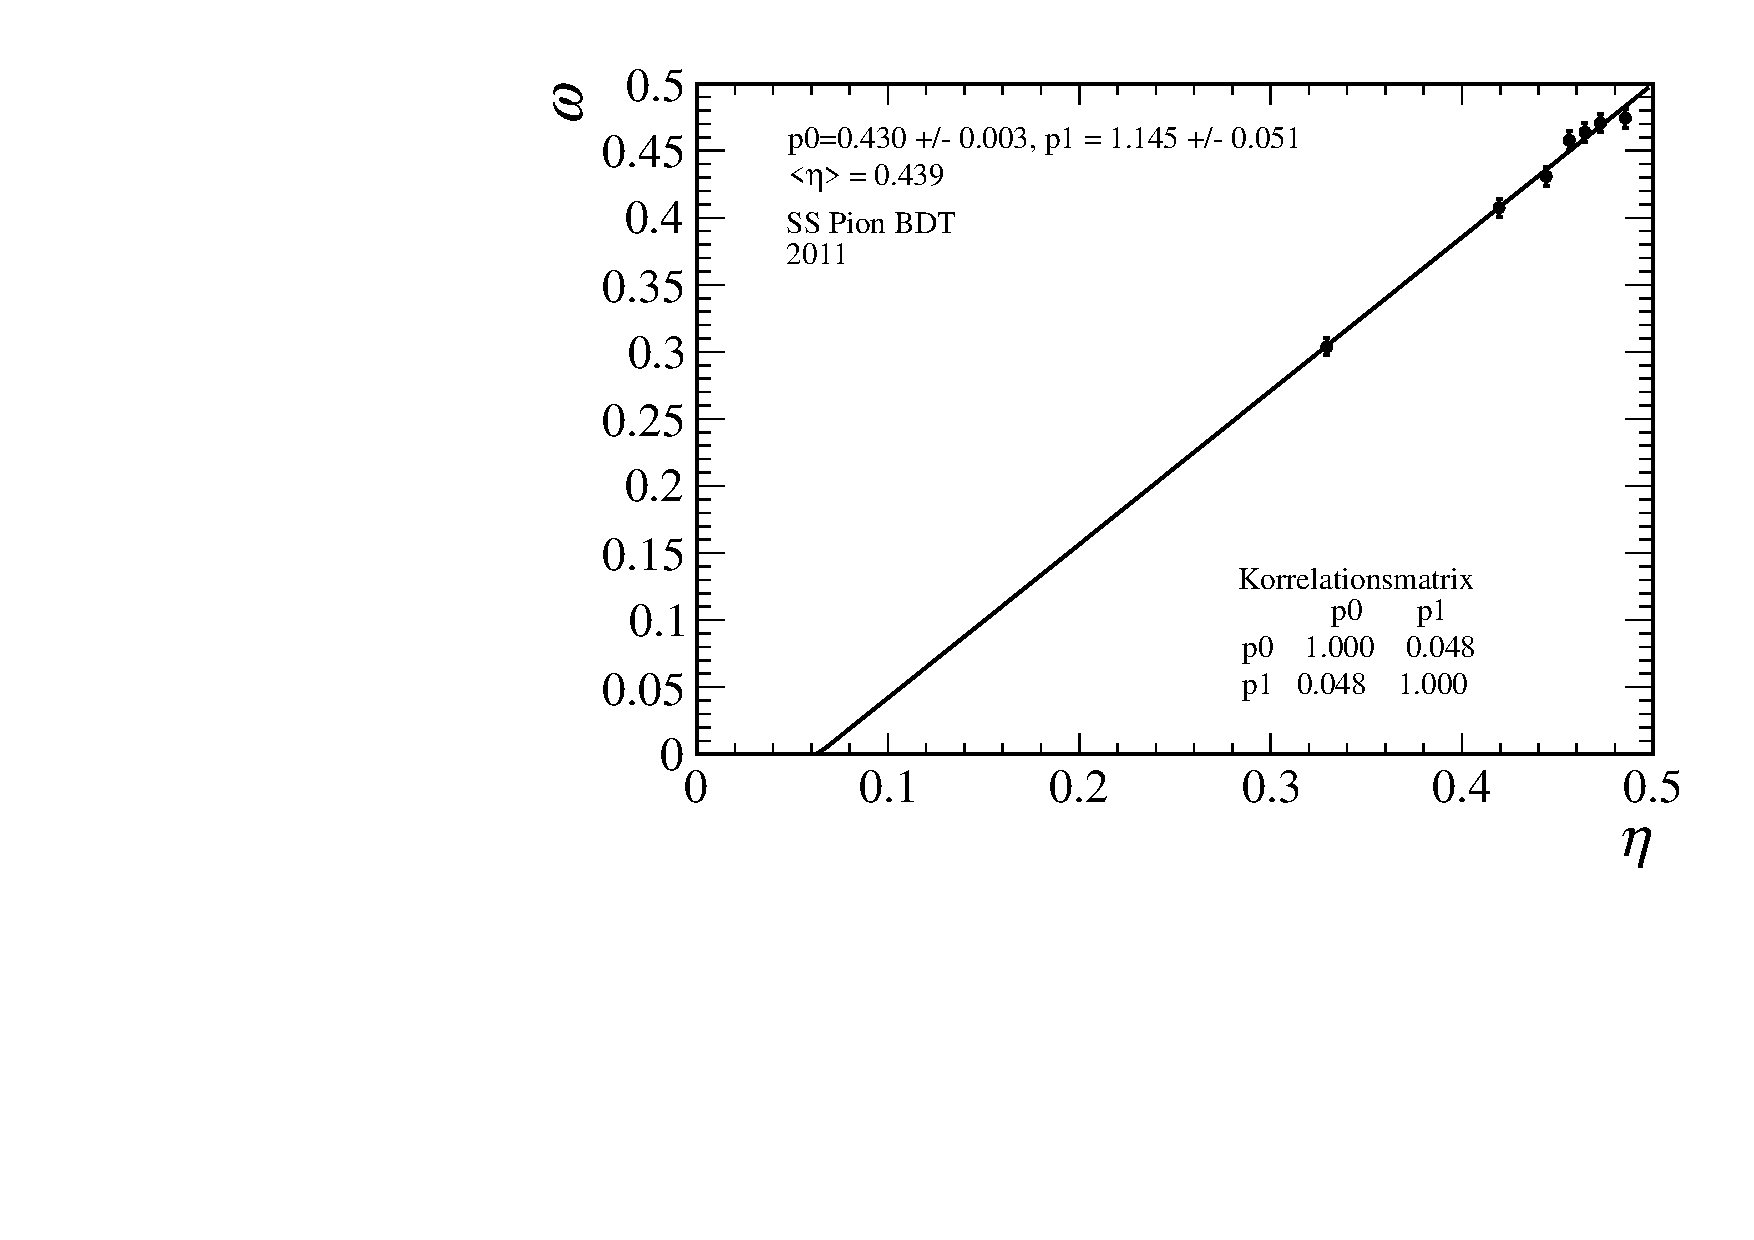
\includegraphics[width=0.49\textwidth]{fig/2011_SSPionBDT.pdf}
		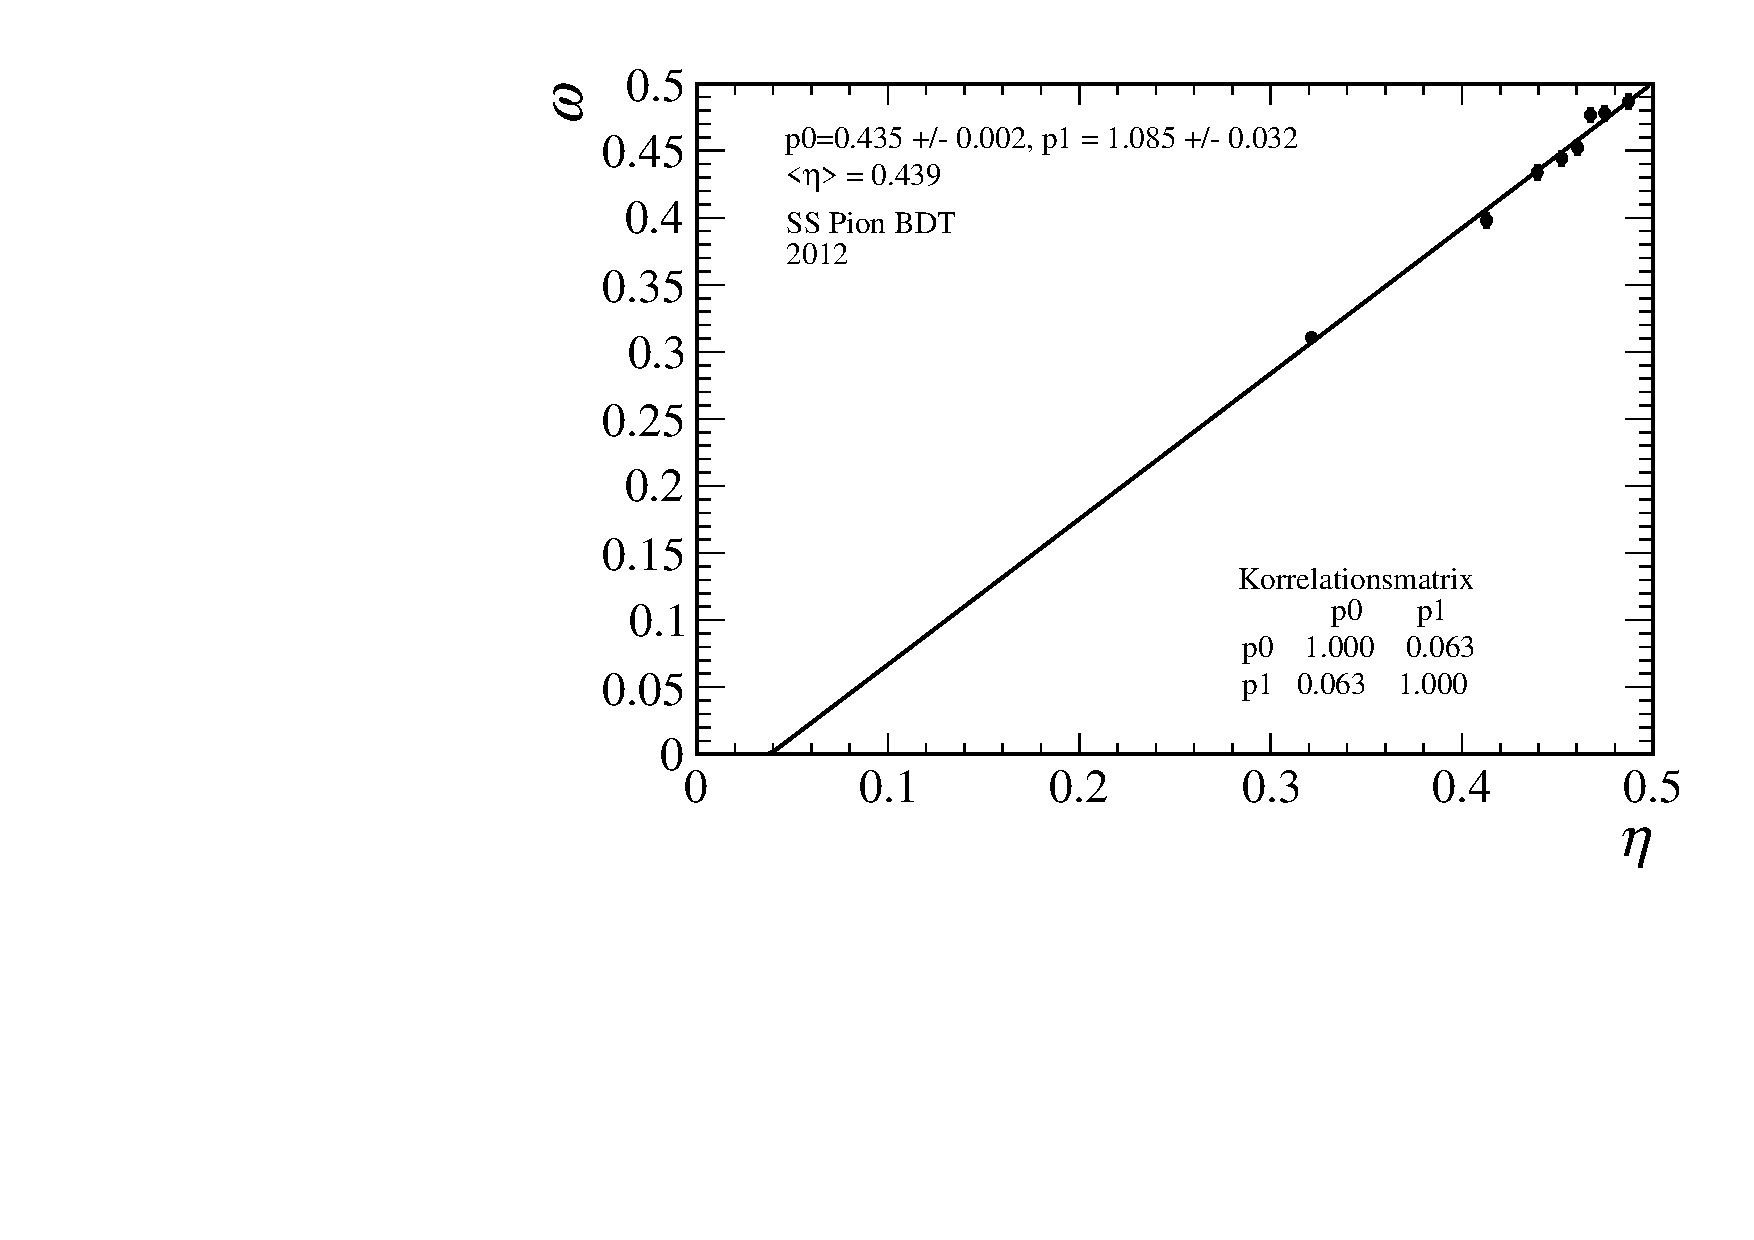
\includegraphics[width=0.49\textwidth]{fig/2012_SSPionBDT.pdf}
	\caption{Fit des linearen Zusammenhangs an die $(\eta,\omega)$-Paare für den SS Pion BDT Tagger auf Daten des Jahres \num{2011} (links) und \num{2012} (rechts).}
	\label{fig:fit_SSPionBDT} 
\end{figure}
\begin{table}[htbp]
	\centering
	\caption{Ergebnisse der Kalibrierung des SS Pion BDT Taggers für die Jahr \num{2011} und \num{2012}.}
	\label{tab:result_SSPionBDT}
	\begin{tabular}{ccccc}
	\toprule
       Jahr & $\langle\eta\rangle$ & $p_0$ & $\left|p_0-\langle\eta\rangle\right|$ & $p_1$ \\ 
       \midrule 
	2011 & $0{.}439$ & $0{.}430\pm0{.}003$ & $0{.}009$ & $1{.}145\pm0{.}051$ \\
   	2012 & $0{.}439$ & $0{.}435\pm0{.}002$ & $0{.}004$ & $1{.}085\pm0{.}032$ \\ 
	\bottomrule
  \end{tabular}
\end{table}
Ebenso ist für das Jahr \num{2011} erkennbar, dass eine größere Anzahl Kategorien keinen großen Nutzen hätte. Auch sind die Parameter $p_0$ und $p_1$ beide um mehr als zwei Standardabweichungen von ihrem ideal kalibrierten Wert entfernt.
\begin{table}[htbp]
	\centering
	\caption{Performanz des SS Pion BDT Taggers für die Jahre \num{2011} und \num{2012}.}
	\label{tab:performance_SSPionBDT}
	\begin{tabular}{ccccc}
	\toprule
      Jahr & $\varepsilon(\%)$ & $\omega$ & $D$ & $\varepsilon D^2(\%)$ \\ 
      \midrule
      2011 & $56{,}797\pm1{,}308$& $0{,}430\pm0{,}003$ & $0{,}140\pm0{,}006$ & $1{,}825\pm0{,}133$\\ 
      2012 & $58{,}147\pm0{,}141$& $0{,}435\pm0{,}002$ & $0{,}130\pm0{,}004$ & $1{,}656\pm0{,}070$\\ 
      \bottomrule
	\end{tabular}
\end{table}\\
Insgesamt lässt sich hier zunächst festhalten, dass der Tagger auf beiden Datensätzen sinnvolle Ergebnisse liefert. Dazu kann man hier die Taggingeffizienz $\varepsilon$ und die effektive Taggingeffizienz $\varepsilon D^2$ betrachten (Tabelle \ref{tab:performance_SSPionBDT}), die für beide Jahre ähnlich sind. Außerdem ist wie bei den zuvor untersuchten Taggern die effektive Taggingeffizienz für das Jahr \num{2012} etwas kleiner. Dies resultiert daraus, dass mit der höheren Rate der Datennahme auch die Selektion der Taggingkandidaten schwieriger und fehleranfäliger wird. Das spiegelt sich in höheren true-mistag-Wahrscheinlichkeiten $\omega$ wieder.\\
Im Vergleich zum schnittbasierten SS Pion Tagger stellt man weiterhin fest, dass der SS Pion BDT Tagger trotz seiner relativ schlechten true-mistag-Wahrscheinlichkeiten $\omega$ insgesamt um etwa \SI{0{,}6}{\%} größere effektive Taggingeffizienzen $\epsilon D^2$ liefert. 

\subsection{Der SS Proton Tagger}

Für den SS Proton Tagger erhält man im Jahr \num{2011} eine Taggingeffizienz von $\varepsilon=\SI{33{,}775}{\%}$ und im Jahr \num{2012} von $\varepsilon=\SI{32{,}588}{\%}$. Die Ergebnisse der Kalibrierung sind in der Abbildung \ref{fig:fit_SSProton} und der Tabelle \ref{tab:result_SSProton} zu sehen. Man sieht auch hier wieder, dass trotz der großen Anzahl getaggter Ereignisse eine größere Anzahl an Kategorien nicht sinnvoll ist, da die mistag-Wahrscheinlichkeiten $\eta$ wieder sehr eng bei Werten größer $\num{0{,}4}$ verteilt sind. Für das Jahr \num{2012} weichen beide Parameter $p_0$ und $p_1$, wie beim SS Pion BDT Tagger, um zwei Standardabweichung von der idealen Kalibrierung ab, 
\begin{figure}[htbp]
	\centering
		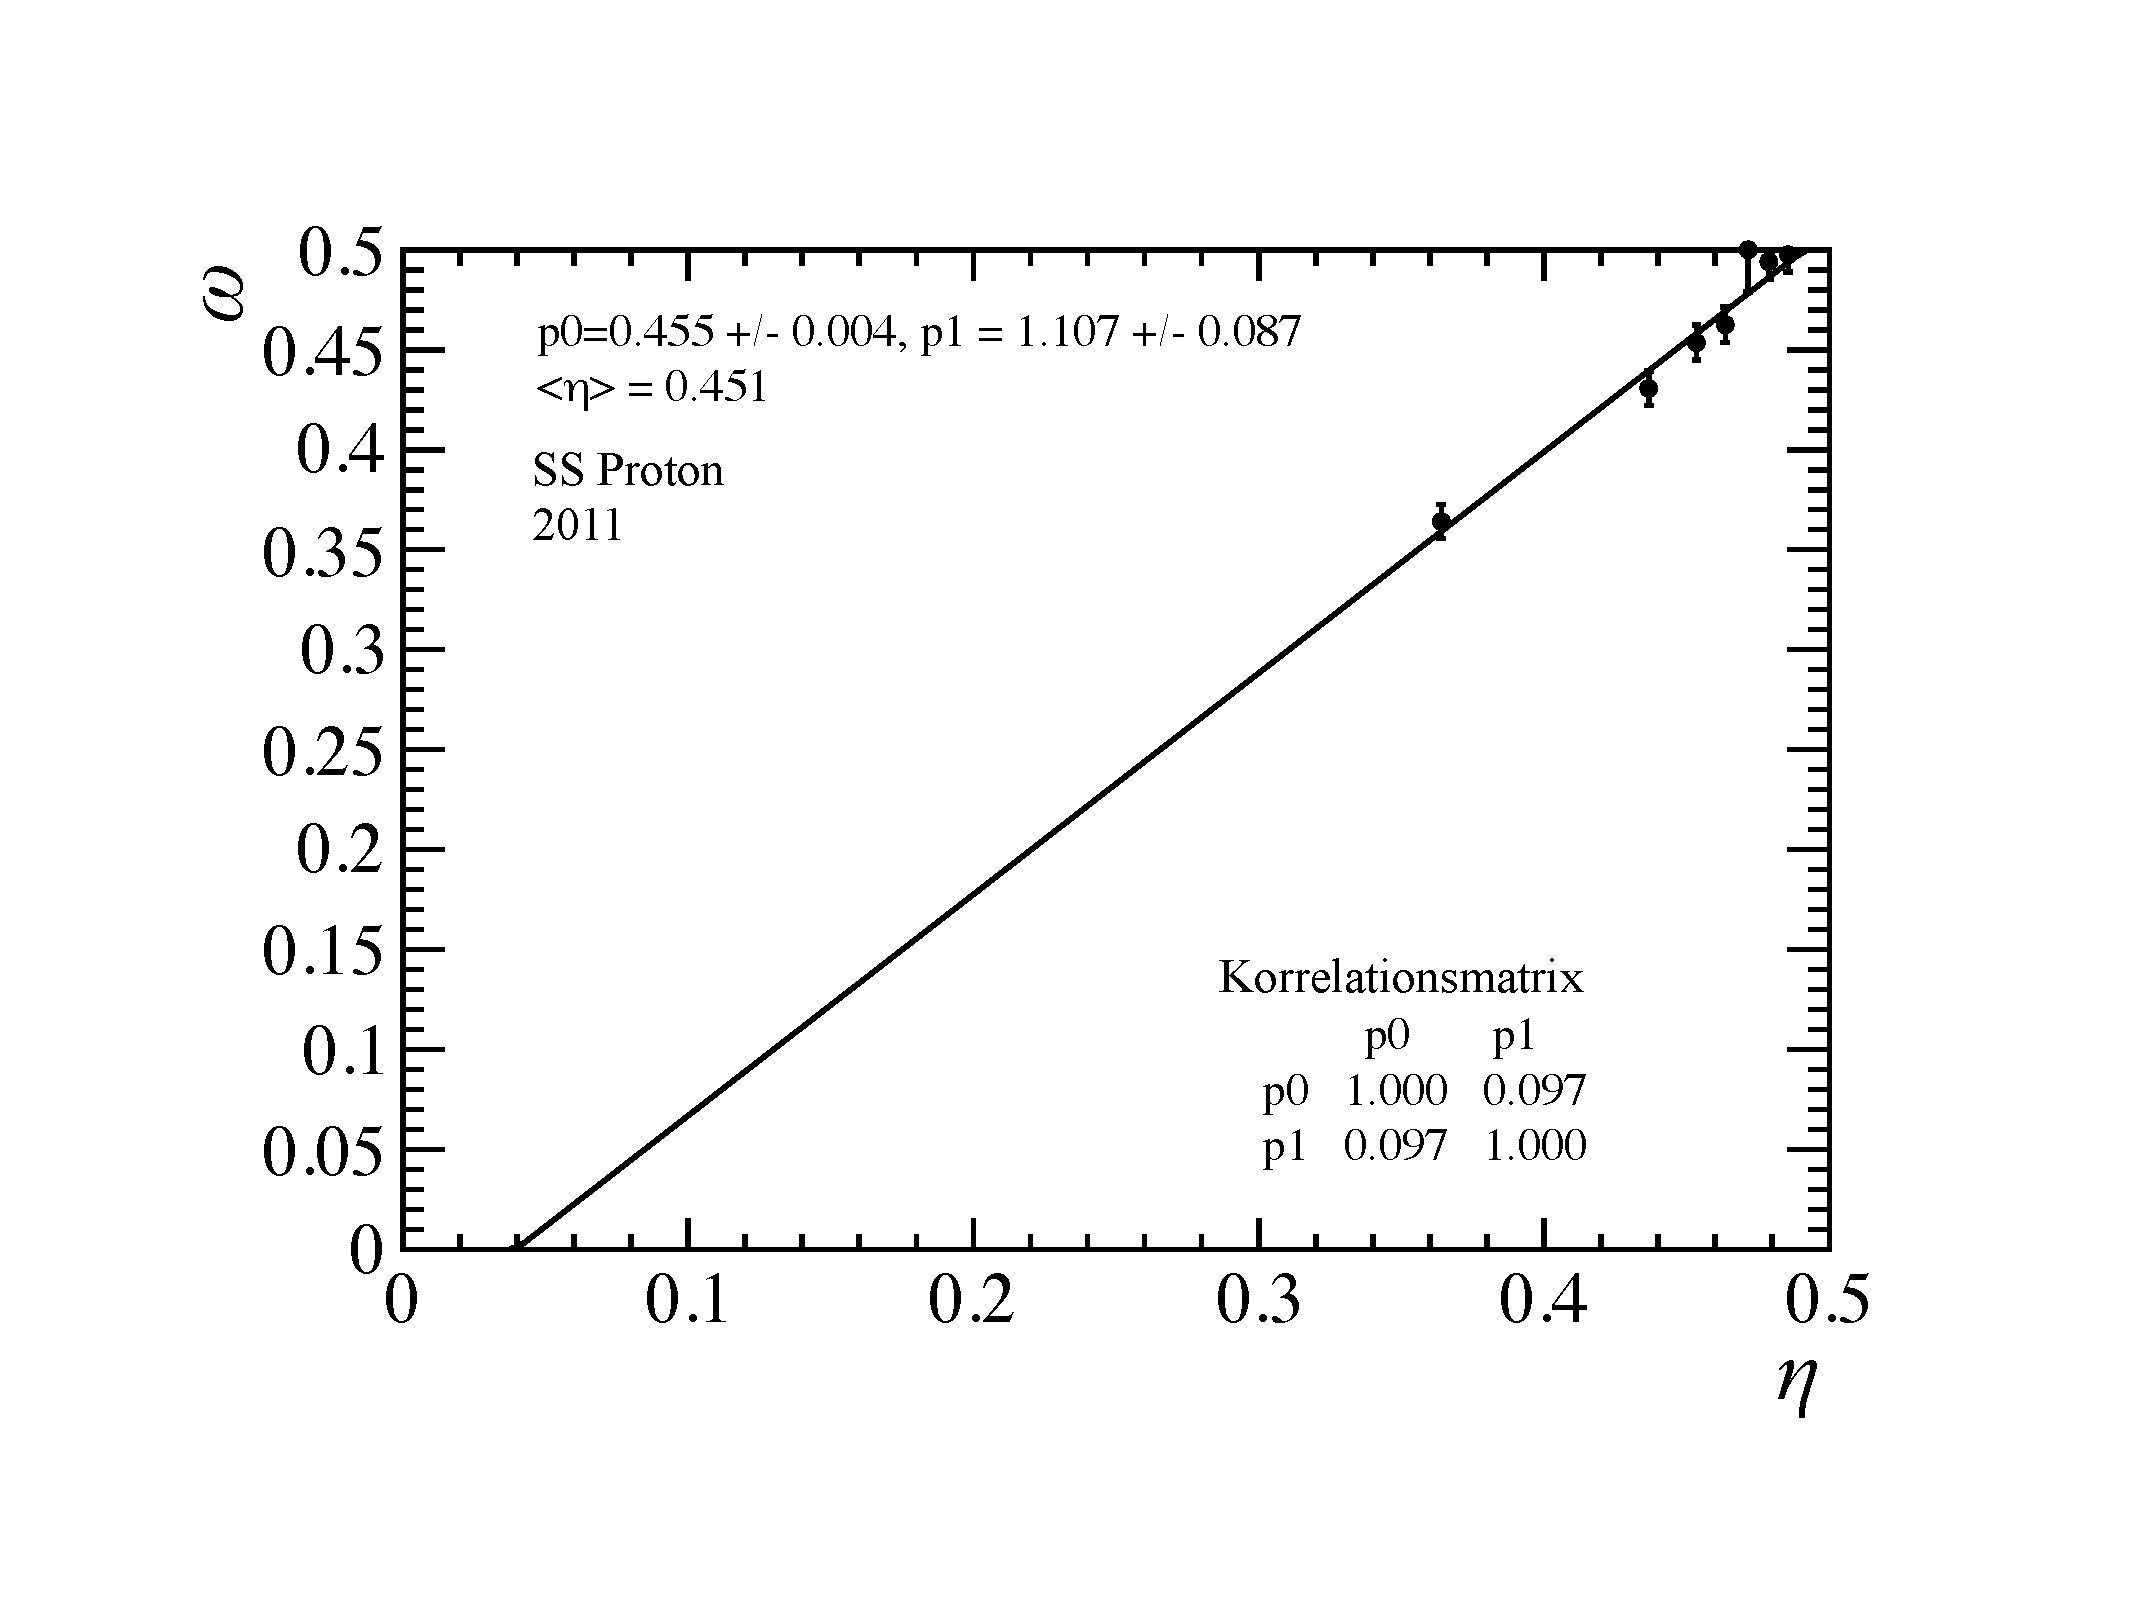
\includegraphics[width=0.49\textwidth]{fig/2011_SSProton.pdf}
		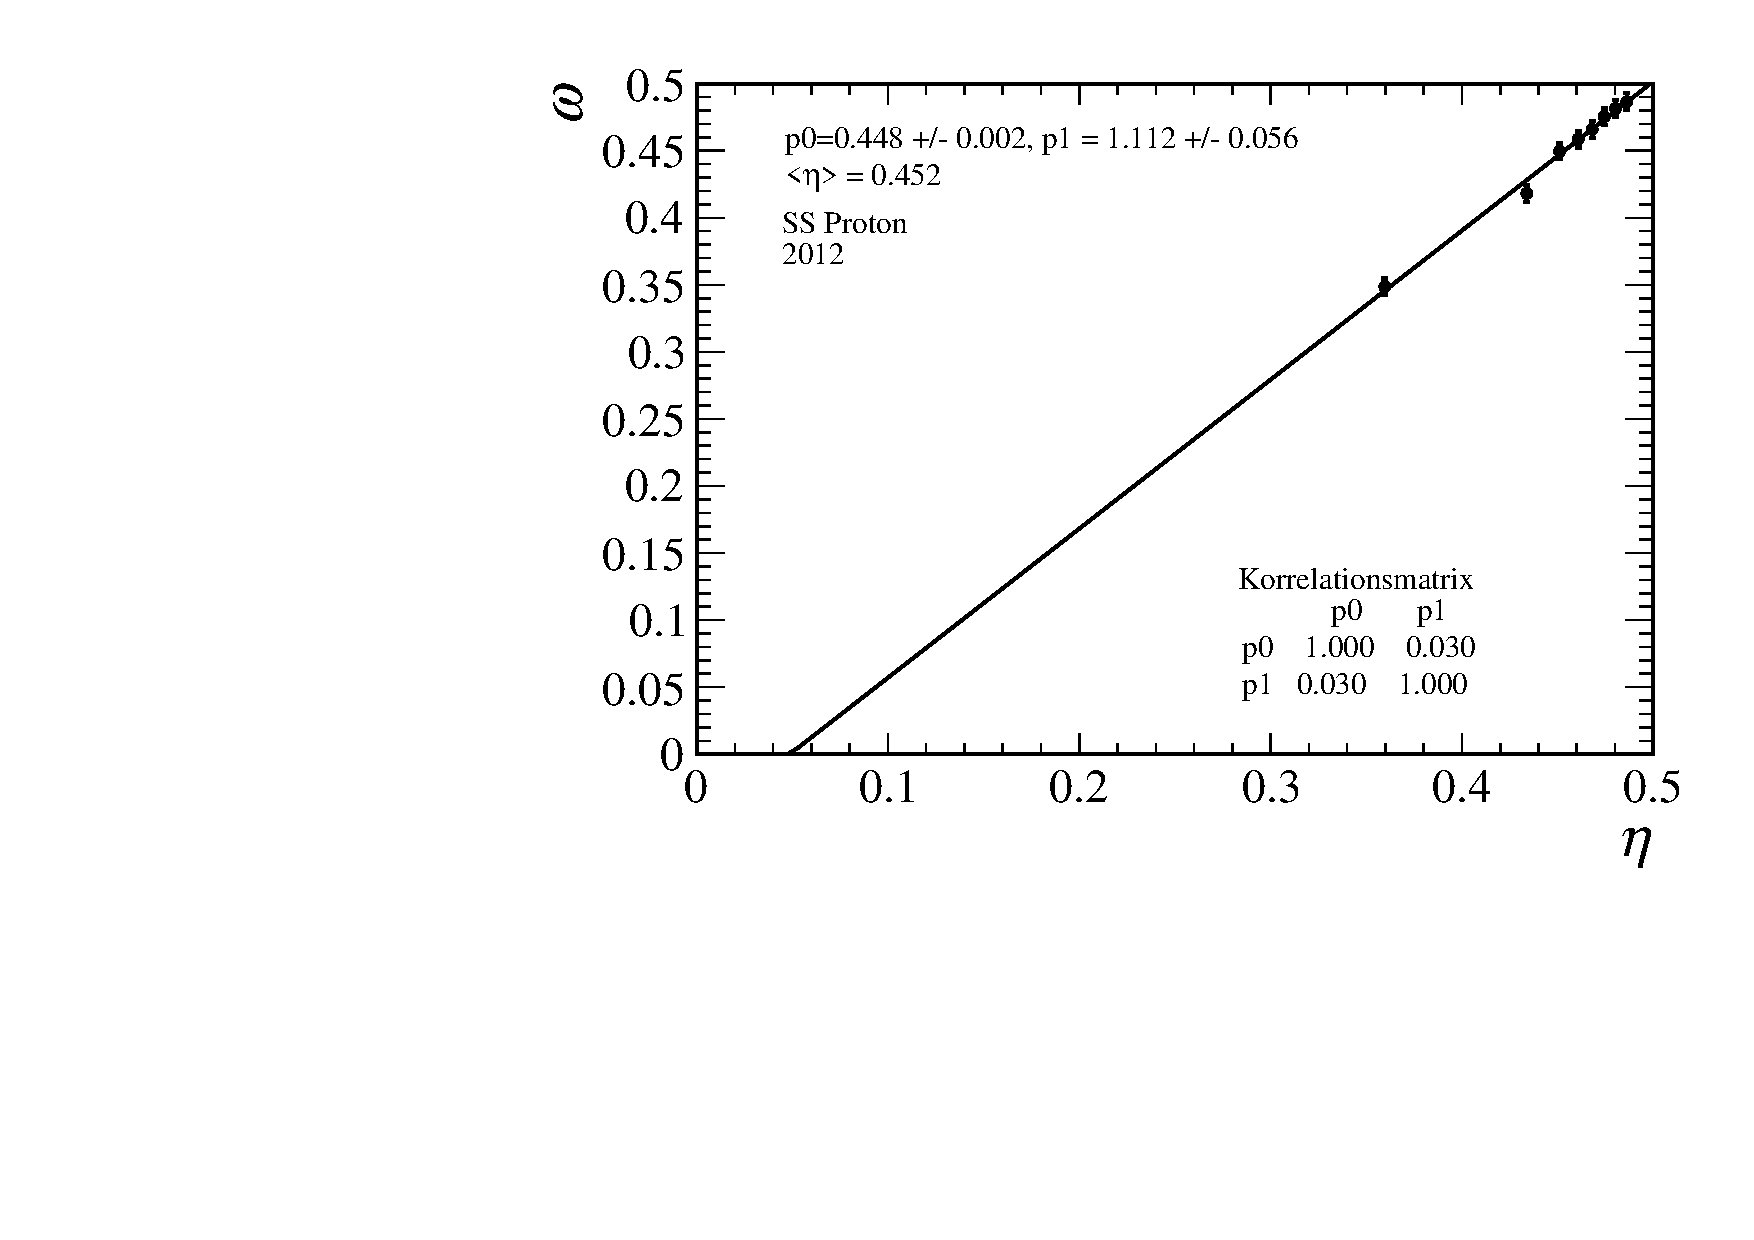
\includegraphics[width=0.49\textwidth]{fig/2012_SSProton.pdf}
	\caption{Fit des linearen Zusammenhangs an die $(\eta,\omega)$-Paare für den SS Proton Tagger auf Daten des Jahres \num{2011} (links) und \num{2012} (rechts).}
	\label{fig:fit_SSProton} 
\end{figure}
während die Abweichungen von der idealen Kalibrierung für das Jahr \num{2011}, aufgrund der größeren statistischen Unsicherheiten auf die Parameter $p_0$ und $p_1$, weniger signifikant sind.
\begin{table}[htbp]
	\centering
	\caption{Ergebnisse der Kalibrierung des SS Proton Taggers für die Jahre \num{2011} und \num{2012}.}
	\label{tab:result_SSProton}
	\begin{tabular}{ccccc}
	\toprule
       Jahr & $\langle\eta\rangle$ & $p_0$ & $\left|p_0-\langle\eta\rangle\right|$ & $p_1$ \\ 
       \midrule
	2011 & $0{.}451$ & $0{.}455\pm0{.}004$ & $0{.}004$ & $1{.}107\pm0{.}087$ \\
   2012 & $0{.}452$ & $0{.}448\pm0{.}002$ & $0{.}004$ & $1{.}111\pm0{.}056$ \\ 
   \bottomrule
	\end{tabular}
\end{table}
\begin{table}[htbp]
	\centering
	\caption{Performanz des SS Proton Taggers für die Jahr \num{2011} und \num{2012}.}
	\label{tab:performance_SSProton}
	\begin{tabular}{ccccc}
	\toprule
       Jahr & $\varepsilon(\%)$ & $\omega$ & $D$ & $\varepsilon D^2(\%)$ \\ 
       \midrule
   2011 & $33{,}775\pm0{,}785$& $0{,}455\pm0{,}003$ & $0{,}090\pm0{,}006$ & $0{,}528\pm0{,}062$\\ 
   2012 & $32{,}588\pm0{,}104$& $0{,}448\pm0{,}002$ & $0{,}104\pm0{,}004$ & $0{,}585\pm0{,}037$\\ 
   \bottomrule
	\end{tabular}
\end{table}
Gleich dem SS Pion BDT Tagger liefert der SS Proton Tagger auf beiden Datensätzen sinnvolle Ergebnisse. Die Taggingeffizienzen $\varepsilon$ und effektiven Taggingeffizienzen $\varepsilon D^2$ (Tabelle \ref{tab:performance_SSProton}) sind in der erwarteten Größenordnung, der mittlere true-mistag $\omega$ ist allerdings für das Jahr \num{2012} bei dem SS Proton Tagger etwas kleiner.

\section{Diskussion der Ergebnisse der Kalibrierung}

Bei der Betrachtung der Ergebnisse lässt sich zunächst die Kalibrierung selbst überprüfen. Um diese in Relation zu den Erwartungen zu setzen muss dabei erwähnt werden, dass bei der verwendeten Version der Flavour-Tagging-Software alle etablierten Tagger bereits kalibriert sein sollten. Die Kalibrierungen wurden dabei jedoch auf neutralen Kanälen wie \BdToJPsiKst oder geladenen Kanälen wie \BuToJPsiKp vorgenommen.\\
Für die Tagger der Opposite Side ist die Kalibrierung unter diesen Bedingungen dabei in fast allen Fällen bestätigt; die Tagger können also in der aktuellen Version der Flavour-Tagging-Software als kalibriert angesehen werden. Einzig die Parameter des OS Kaon nnet weichen auf dem Datensatz aus dem Jahr \num{2012} beide so stark von den Erwartungen eines ideal kalibrierten Taggers ab, dass sich hier bei Analysen die diesen Tagger verwenden Probleme ergeben könnten. Bei den Taggern der Same Side ist zunächst etwas überraschend, dass der SS Pion Tagger auf dem hier untersuchten Kanal in beiden Jahren nicht kalibriert ist, da auch für diesen eine Präkalibration durchgeführt wurde. Allerdings sind bei den Taggern der Same Side auch durchaus größere Unterschiede zu erwarten, weil die Tagger stärker vom Signalzerfall beeinflusst sind. Da es sich bei den beiden auf \BdToDpi entwickelten Taggern, dem SS Pion BDT und dem SS Proton Tagger an dieser Stelle um die ersten unabhängigen Gegenproben handelt, liegt der Fokus hier weniger auf einer idealen Kalibration. Nachdem in der Entwicklung anfangs Probleme auftraten, und beide Tagger nicht wie gewünscht funktionierten, scheinen diese nun behoben worden zu sein. Bei beiden Taggern liefert die Kalibrierung sinnvolle Ergebnisse für die Taggingeffizienz $\varepsilon$ und die effektive Taggingeffizienz $\varepsilon D^2$. Außerdem lässt sich an dieser Stelle ein erster Vergleich zwischen dem SS Pion und dem SS Pion BDT Tagger ziehen. Hier sieht man, dass der SS Pion BDT Tagger in der effektiven Taggingeffizienz $\varepsilon D^2$ einen Zuwachs bringt. Einzig herausfordernd wären hier mögliche größere Korrelationen des SS Pion BDT Taggers gegenüber dem SS Pion Tagger mit anderen Taggern.\\
Weiterhin lassen sich die Tagger bezüglich ihrer effektiven Taggingeffizienzen $\varepsilon D^2$ vergleichen. Obwohl bei allen Taggern die Taggingeffizienz $\varepsilon$ etwa gleich bleibt, ist hier zu erkennen, dass bis auf den SS Proton hier bei alle Taggern  $\varepsilon D^2$ für die Daten des Jahres \num{2012} im Vergleich zu den Daten des Jahres \num{2011} sinkt (Tabelle \ref{tab:diskussion}). Eine mögliche Ursache ist die höhere instantane Luminosität im Jahr \num{2012}. Durch die größere Anzahl an Protonenkollisionen bei einer einzelnen Strahlkollision ist es für die Taggingalgorithmen schwieriger ihre Taggingteilchen zu finden. Somit verschlechtern sich die Einschätzungen der Tagger, was sich direkt im true-mistag $\omega$ niederschlägt. Auch dieser Effekt, der schlechter werdenden true-mistag-Wahrscheinlichkeiten ist in den Ergebnissen zu erkennen. Einzig die Abweichung im Verhalten des SS Proton Taggers muss noch weiter untersucht werden.
\begin{table}[htbp]
	\centering
	\caption{Zusammenfassung der Ergebnisse der Taggingeffizienzen $\varepsilon$ und der effektiven Taggingeffizienzen $\varepsilon D^2$ der Kalibrierungen.}
	\label{tab:diskussion}
	\begin{tabular}{ccccc}
	\toprule
       		& \multicolumn{2}{c}{$\varepsilon(\%)$} & \multicolumn{2}{c}{$\varepsilon D^2(\%)$}\\
		& \num{2011} & \num{2012} & \num{2011} & \num{2012} \\ 
		\midrule
   OS Std. Komb. & $37{,}449\pm0{,}814$& $38{,}366\pm0{,}112$ & $3{,}777\pm0{,}183$ & $3{,}597\pm0{,}091$\\ 
   OS Charm & $3{,}304\pm0{,}102$& $3{,}264\pm0{,}032$ & $0{,}512\pm0{,}049$ & $0{,}395\pm0{,}041$\\ 
   OS Kaon nnet & $45{,}044\pm1{,}041$& $46{,}459\pm0{,}125$ & $1{,}621\pm0{,}122$ & $1{,}588\pm0{,}061$\\ 
   SS Pion & $14{,}847\pm0{,}380$& $15{,}146\pm0{,}070$ & $1{,}104\pm0{,}074$ & $1{,}071\pm0{,}049$\\ 
   SS Pion BDT & $56{,}797\pm1{,}308$& $58{,}147\pm0{,}141$ & $1{,}825\pm0{,}133$ & $1{,}656\pm0{,}070$\\ 
   SS Proton & $33{,}775\pm0{,}785$& $32{,}588\pm0{,}104$ & $0{,}528\pm0{,}062$ & $0{,}585\pm0{,}037$\\ 
   \bottomrule
   \end{tabular}
\end{table}

\section{Korrelation zwischen Taggern der Same Side}

Der neue SS Proton Tagger untersucht, wie der etablierte SS Pion oder auch auch der neue SS Pion BDT Tagger, den Hadronisierungsprozess eines \dquark-Quarks auf der Same Side. Aufgrund dieser Ähnlichkeit soll zwischen diesen Taggern, vor allem zwischen dem SS Proton Tagger und den beiden Pionen Taggern die Möglichkeit einer bestehenden Korrelation untersucht werden. Eine mögliche Korrelation bestünde, wenn im Hadronisierungsprozess des Pions auf der Same Side direkt ein Proton entsteht. Dieses würde für den SS Proton Tagger zur gleichen Entscheidung führen wie das Pion für den SS Pion Tagger. Um dabei zunächst einen Einblick zu erhalten, wie stark diese Korrelation sein kann, wird das Verhältnis an Ereignissen $R_\text{Überlapp}$ berechnet, bei der beide Tagger für dieselben Ereignisse eine Entscheidung treffen, relativ zur Gesamtzahl der von beiden Taggern getroffenen Entscheidungen:
\begin{equation}
R_\text{Überlapp}=\frac{N_{\pi+\proton}}{N_{\pi,exkl}+N_{\proton,exkl}+N_{\pi+\proton}}.
\end{equation}
Dabei bezeichnet $N_{\pi+\proton}$ die Anzahl Ereignisse, in der sowohl der entsprechende Pion Tagger eine Entscheidung getroffen hat, als auch der SS Proton Tagger und $N_{\pi,exkl}$ und $N_{\proton,exkl}$ sind die Anzahl Ereignisse, in denen der entsprechende Pionen Tagger beziehungsweise der SS Proton Tagger jeweils exklusiv eine Entscheidung getroffen haben. Für den Vergleich zwischen dem SS Pion Tagger und dem SS Proton Tagger erhält man so $R_\text{Überlapp}=\SI{11{,}89}{\%}$ und für den Vergleich zwischen SS Pion BDT Tagger und SS Proton Tagger ein Verhältnis von $R_\text{Überlapp}=\SI{31{,}18}{\%}$. Eine mögliche Korrelation wäre also zwischen dem SS Pion BDT Tagger und dem SS Proton Tagger schwerwiegender als zwischen dem SS Proton Tagger und dem SS Pion Tagger.\\
Im nächsten Schritt wird betrachtet, wie oft beide Tagger jeweils gleiche  oder unterschiedliche Entscheidungen treffen. Die Ergebnisse dazu sind in Tabelle \ref{tab:overlap} dargestellt. Man erkennt, dass auch hier die Anzeichen aufgrund der etwas größeren Diskrepanz zwischen gleichen und unterschiedlichen Entscheidungen für eine mögliche Korrelation zwischen dem SS Pion BDT und dem SS Proton Tagger stärker sind, als bei dem SS Pion und dem SS Proton Tagger. Zum Vergleich ist weiterhin der Überlapp $R_\text{Überlapp}$ zwischen dem SS Pion und dem SS Pion BDT Tagger gezeigt. Bei diesen beiden Taggern erwartet man eine nahezu vollständige Korrelation, da sie die gleichen Teilchen für ihre Tagentscheidung nutzen.
\begin{table}[htbp]
	\centering
	\small
	\caption{Verhältnis gleicher und unterschiedlicher Entscheidungen zur Einschätzung der Korrelation. Die absoluten Anzahlen werden dabei durch $N$ bezeichnet, die relativen Verhältnisse zum gesamten Überlapp der beiden Tagger jeweils mit $R$. Weiterhin bezeichnet $d_i=d_j$ die Fälle mit gleichen Tags und $d_i\neq d_j$ die Fälle mit ungleichen Tags.}
	\label{tab:overlap}
	\begin{tabular}{ccccccc}
	\toprule
         			& \multicolumn{2}{c}{SS$_\pi$ \& SS$_\proton$} & \multicolumn{2}{c}{SS$_{\pi\text{BDT}}$ \& SS$_\proton$} & \multicolumn{2}{c}{SS$_\pi$ \& SS$_{\pi\text{BDT}}$} \\  
        				& $N$ & $R \si{ [\percent]}$ & $N$ & $R \si{ [\percent]}$ & $N$ & $R \si{ [\percent]}$ \\ 
				\midrule
       $d_i=d_j$	& $9562\pm98$ & $51{,}2\pm0{,}6$ & $42360\pm206$ & $53{,}1\pm0{,}3$ &  $46338\pm215$  & $90{,}6\pm0{,}6$ \\ 
        $d_i\neq d_j$  & $9096\pm95$ & $48{,}8\pm0{,}6$ & $37418\pm193$ & $46{,}9\pm0{,}3$ & $4799\pm69$  & $9{,}4\pm0{,}1$ \\ 
        \bottomrule
	\end{tabular}
\end{table}\\
Man erkennt hier, dass Anzeichen für eine leichte Korrelation vor allem zwischen SS Pion BDT und SS Proton Tagger bestehen, da das Verhältnis $R$ signifikant von \SI{50}{\%} abweicht.\\
Im Folgenden werden nun Korrelationen zwischen den Verteilungen der mistag-Wahrscheinlichkeiten $\eta$ gegeneinander untersucht. Zum Vergleich ist hier  die Kombination aus SS Pion und SS Pion BDT Tagger für zwei stark korrelierte Tagger und die Kombination aus SS Pion Tagger und der OS Kombination für zwei unkorrelierte Tagger gezeigt. In den Abbildungen \ref{fig:SSp_SSpi}, \ref{fig:SSp_SSpiBDT}, \ref{fig:SSpi_SSpiBDT} und \ref{fig:SSpi_OS} sind die Vergleiche der 2D-mistag-Verteilungen dargestellt. Bei einer starken Korrelation erwartet man, wie für den Vergleich des SS Pion und des SS Pion BDT Taggers zu sehen, diagonale Strukturen. Für die Kombinationen des SS Proton Taggers mit den beiden Pionen Taggern ist aber vor allem eine gleichmäßige Verteilung der mistag-Wahrscheinlichkeiten um eine Häufung in der oberen rechten Eckte der Plots zu erkennen. Die waagerechten und senkrechten Strukturen die teilweise zu sehen sind, deuten nicht auf eine Korrelation, sondern auf spezielle Ausprägungen der einfachen mistag-Verteilungen hin.
\begin{figure}[htbp]
	\centering
		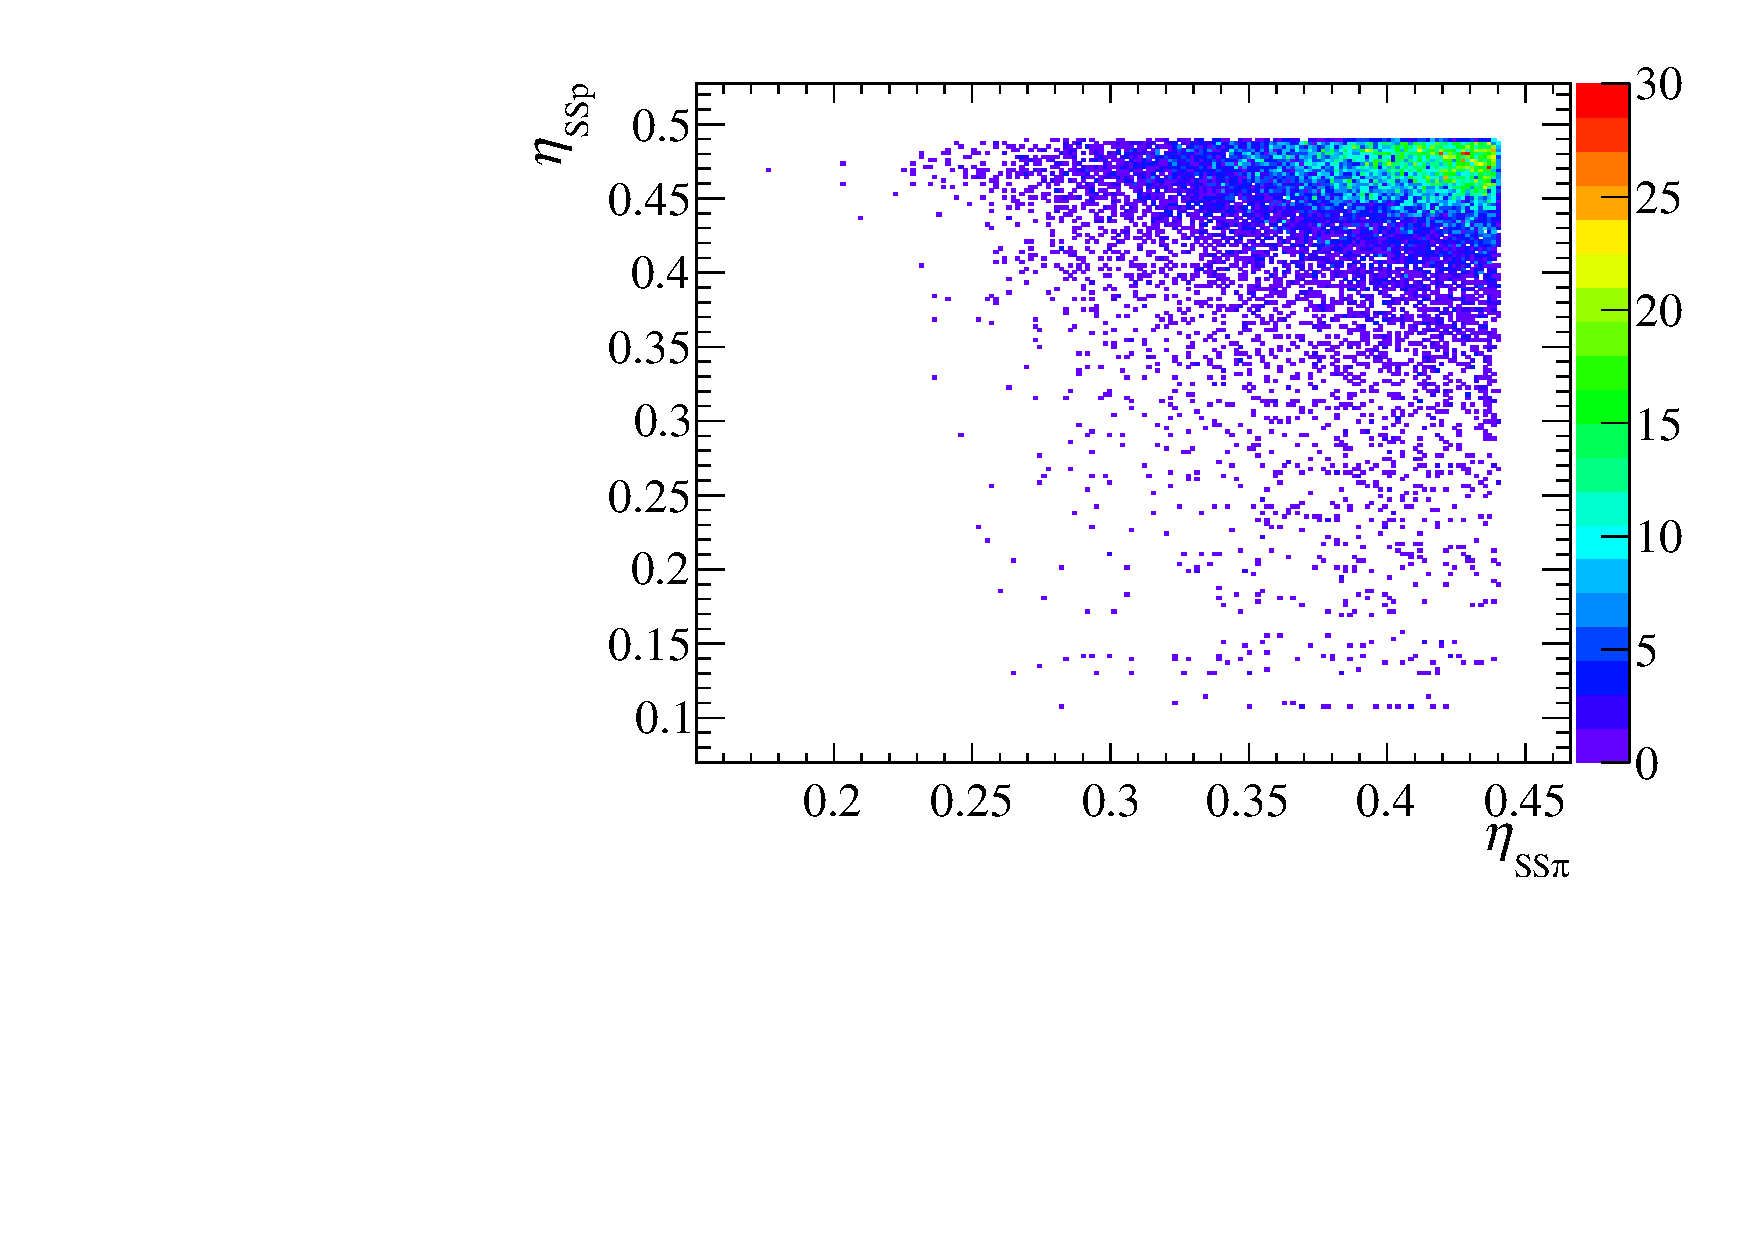
\includegraphics[width=0.75\textwidth]{fig/SSp_SSpi.pdf}
	\caption{Zweidimensionale Darstellung der $\eta$-Verteilungen des SS Proton und des SS Pion Taggers. Es sind keine diagonalen Strukturen, die auf eine Korrelation schließen lassen, erkennbar.}
	\label{fig:SSp_SSpi} 
\end{figure}
\begin{figure}[htbp]
	\centering
		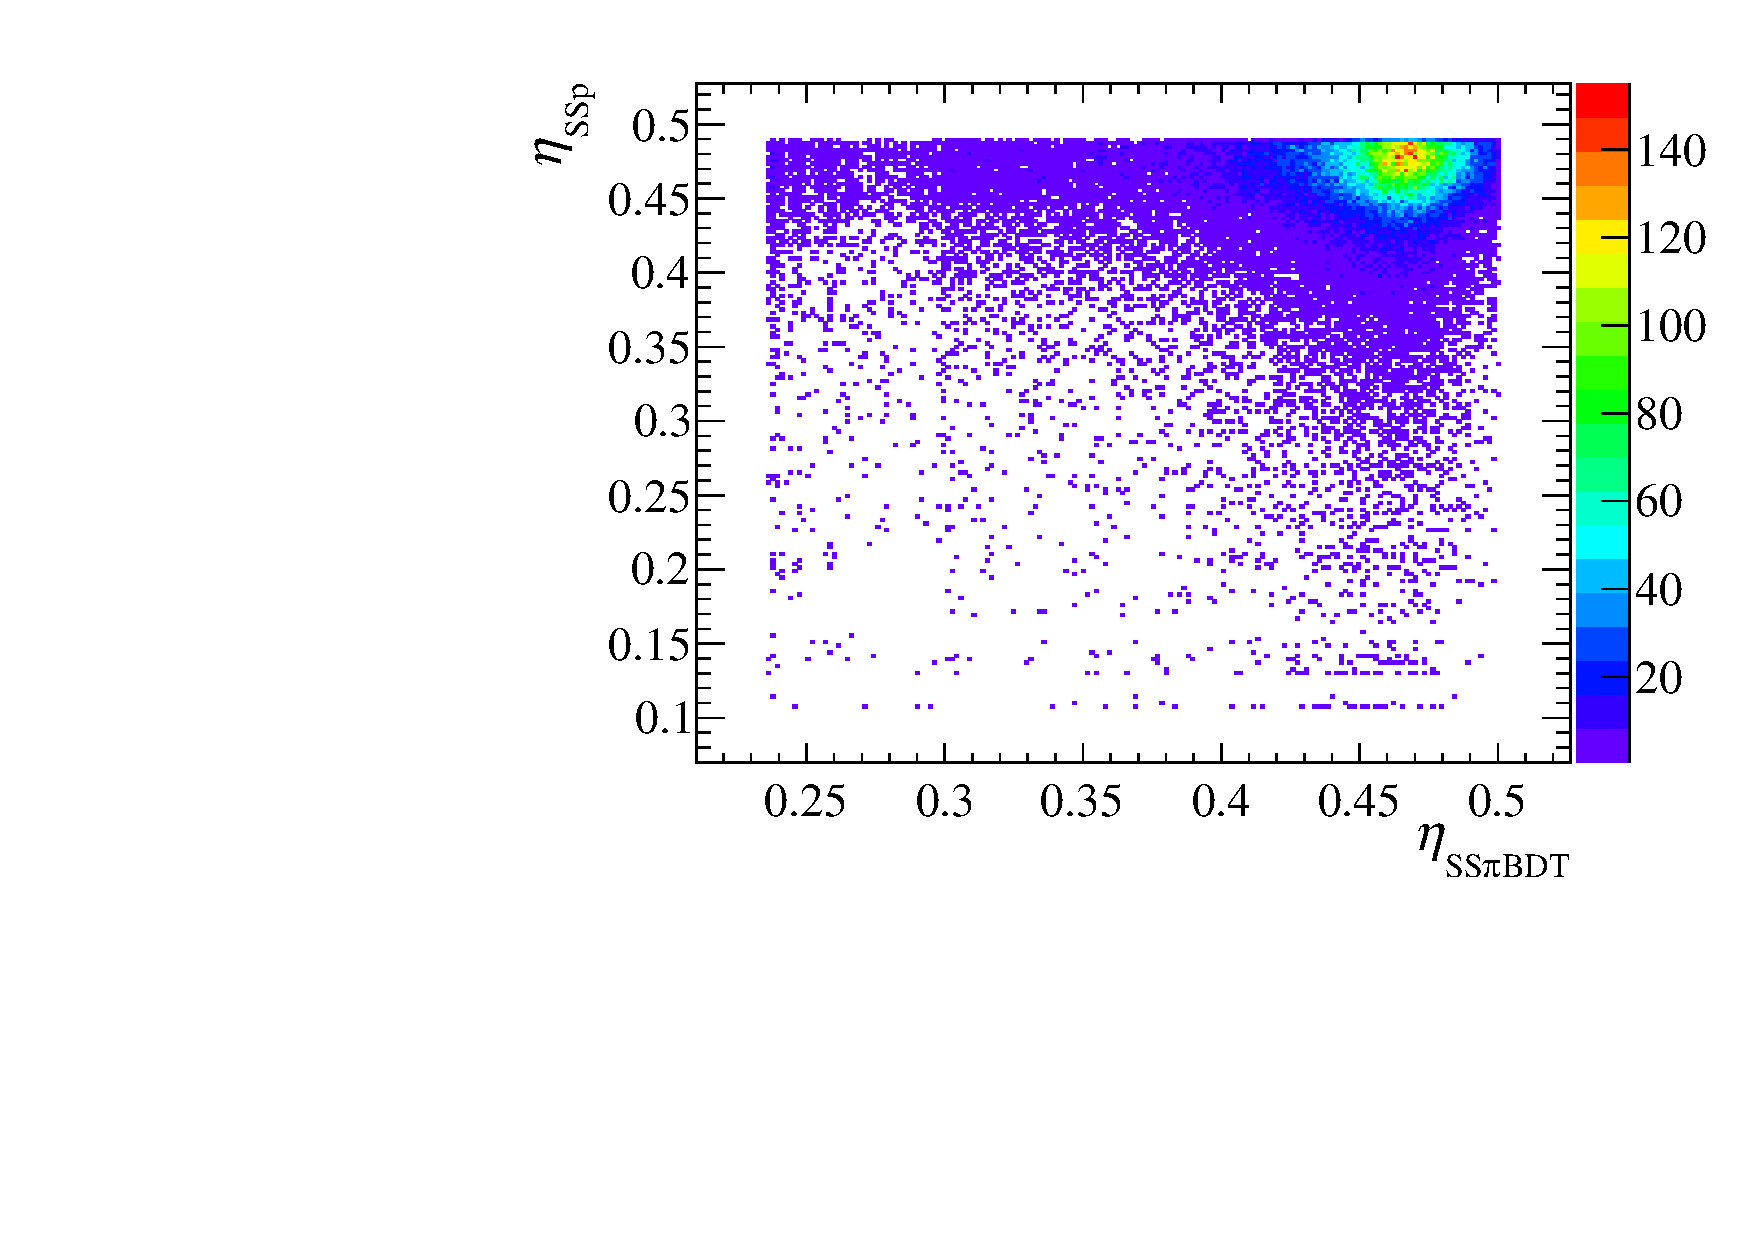
\includegraphics[width=0.75\textwidth]{fig/SSp_SSpiBDT.pdf}
	\caption{Zweidimensionale Darstellung der $\eta$-Verteilungen des SS Proton und des SS Pion BDT Taggers. Es sind keine diagonalen Strukturen, die auf eine Korrelation schließen lassen, erkennbar.}
	\label{fig:SSp_SSpiBDT} 
\end{figure}
\begin{figure}[htbp]
	\centering
		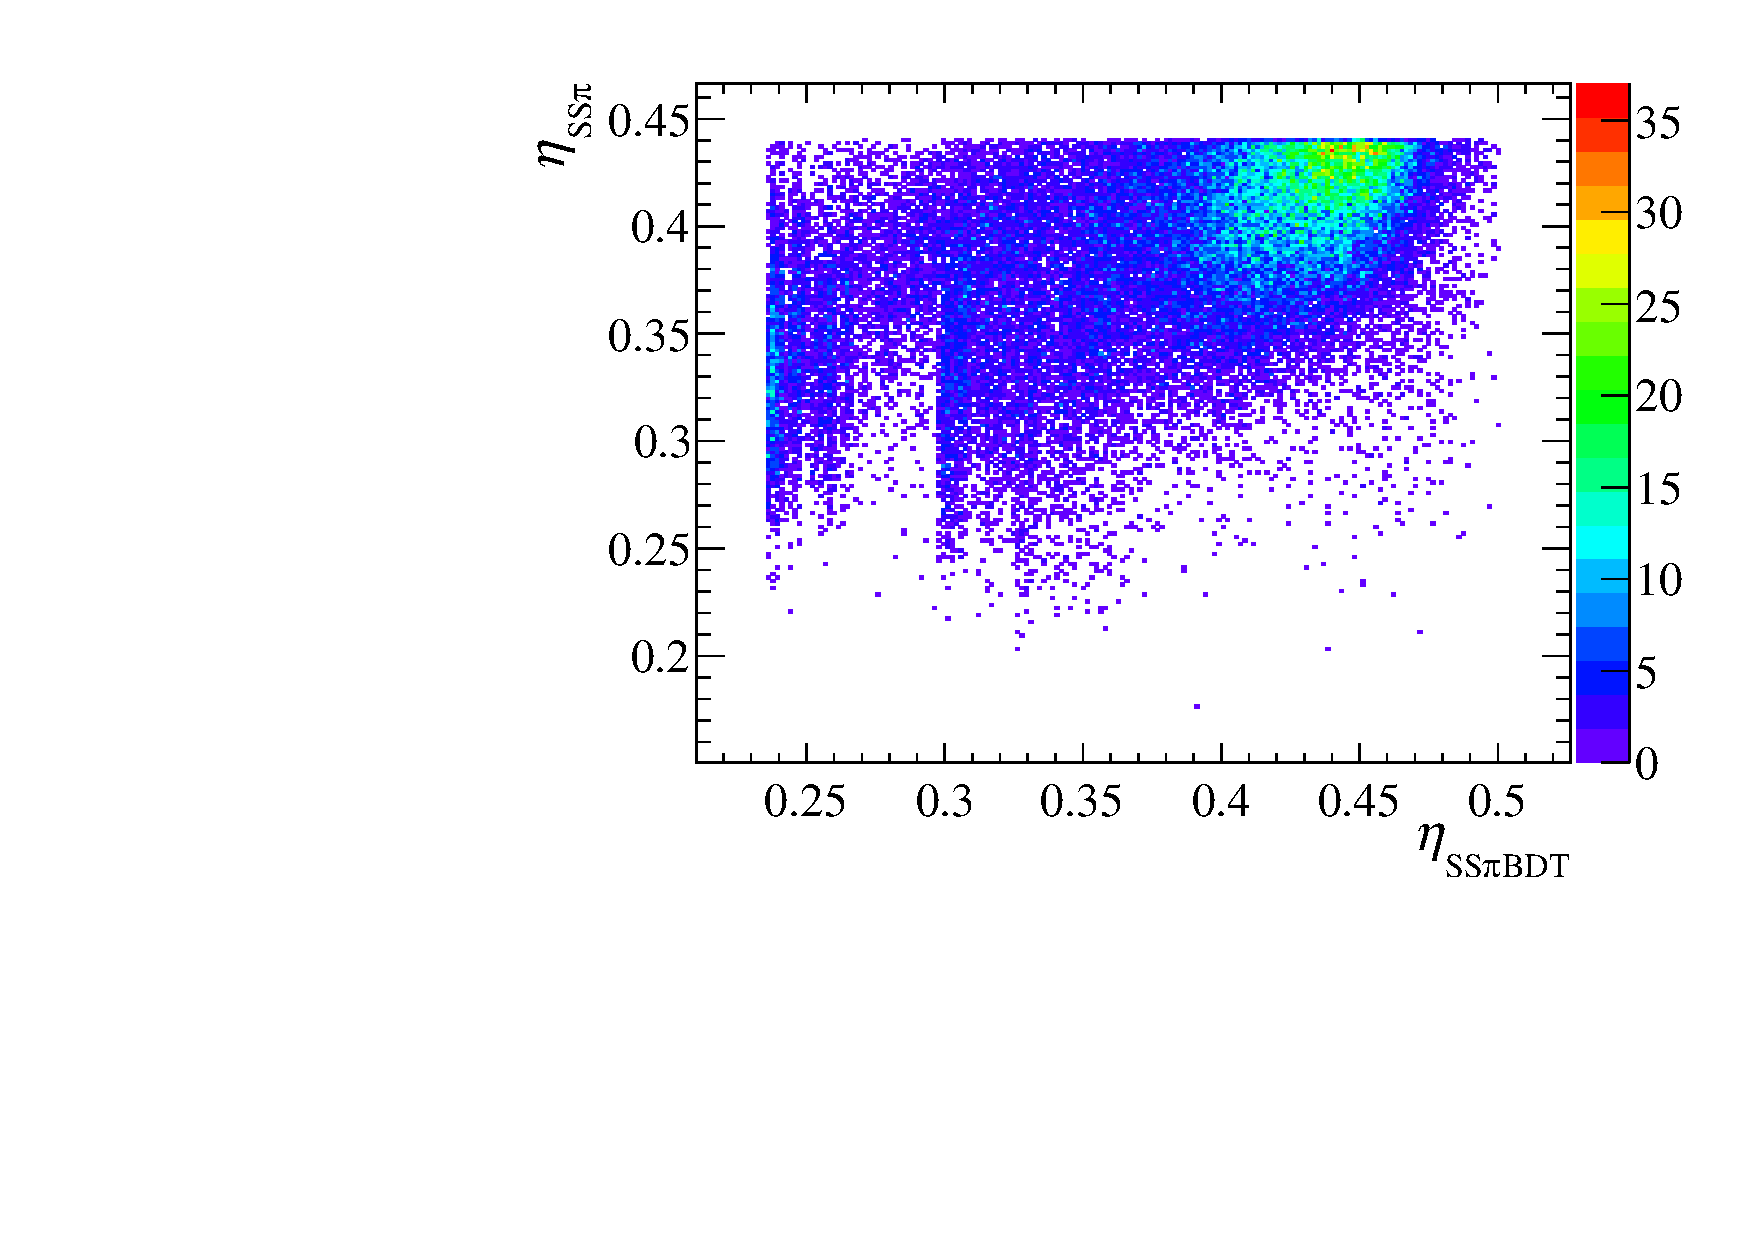
\includegraphics[width=0.75\textwidth]{fig/SSpi_SSpiBDT.pdf}
	\caption{Zweidimensionale Darstellung der $\eta$-Verteilungen des SS Pion BDT und des SS Pion Taggers. Es sind diagonalen Strukturen, die auf eine Korrelation schließen lassen, erkennbar.}
	\label{fig:SSpi_SSpiBDT} 
\end{figure}
\begin{figure}[htbp]
	\centering
		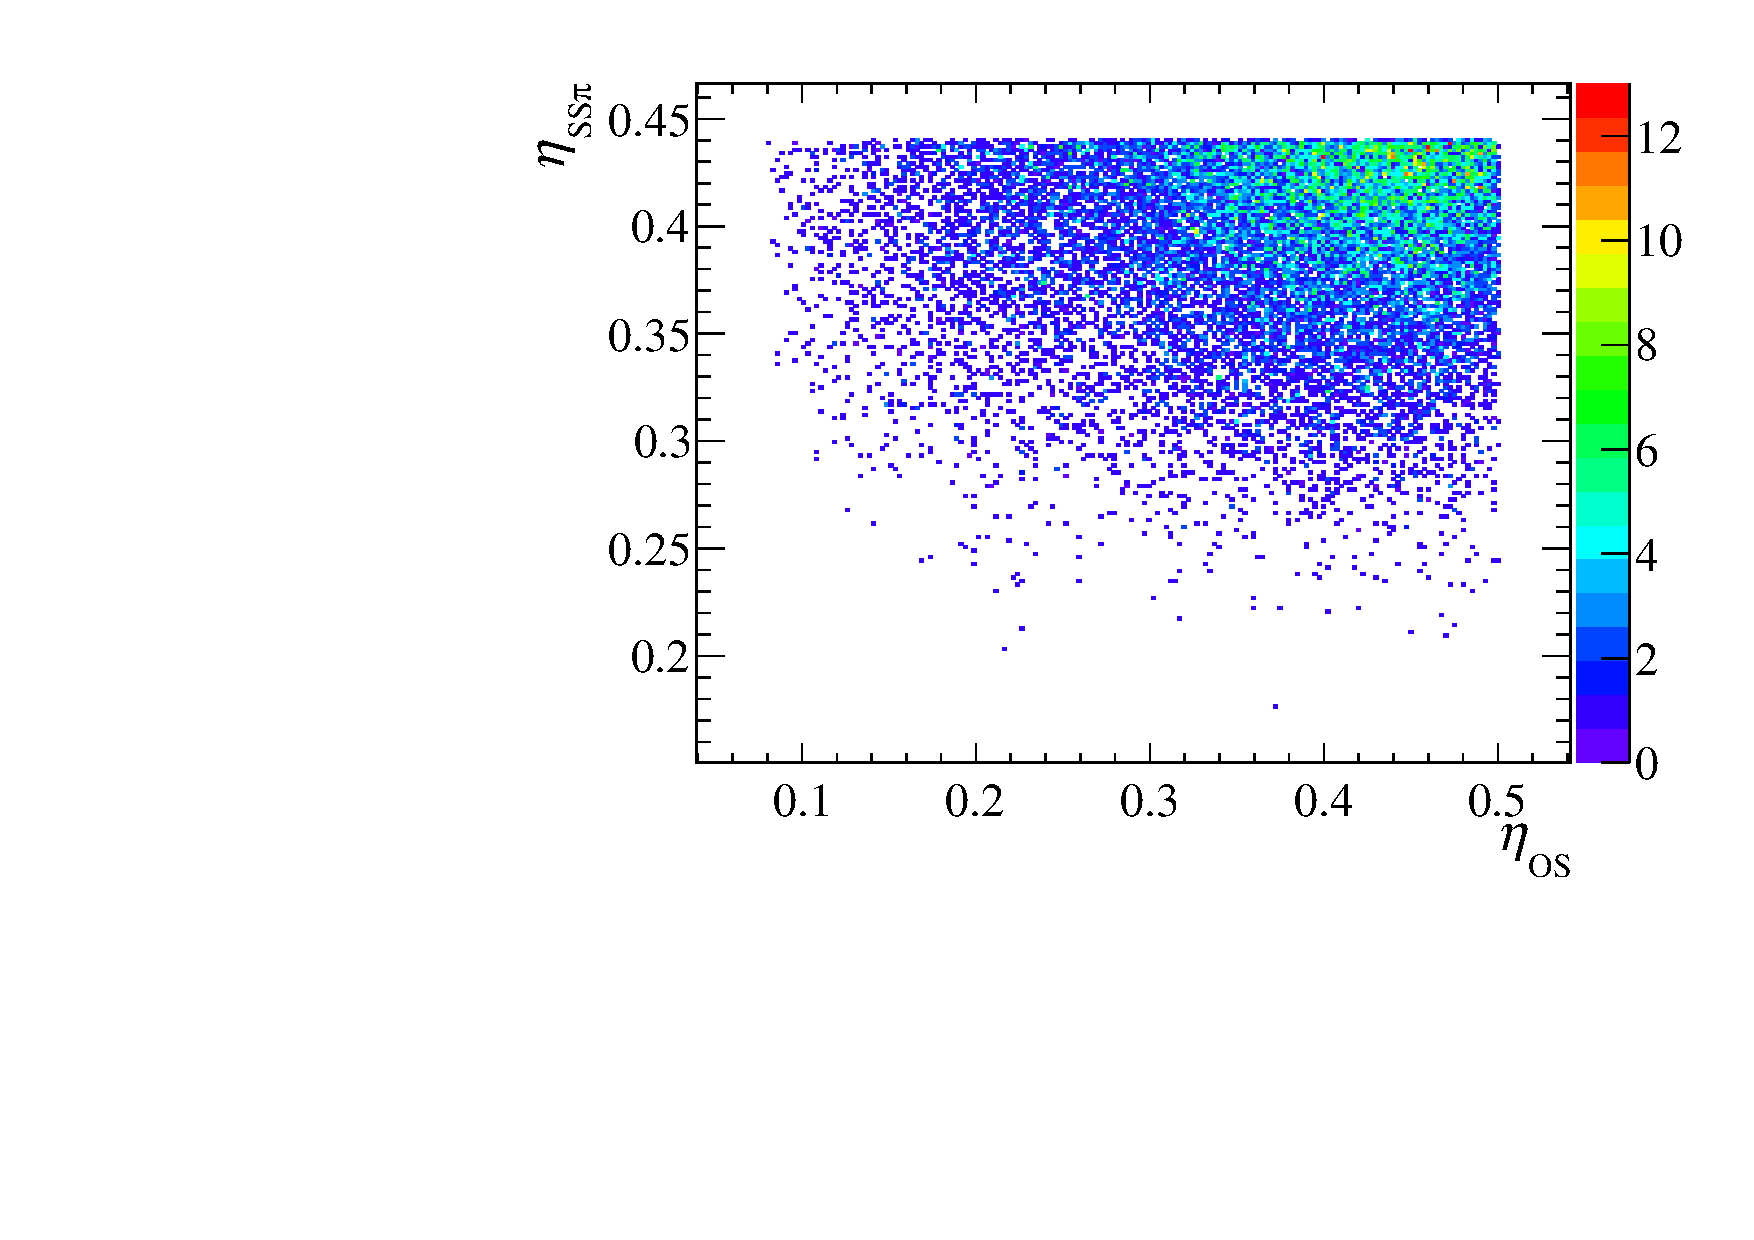
\includegraphics[width=0.75\textwidth]{fig/SSpi_OS.pdf}
	\caption{Zweidimensionale Darstellung der $\eta$-Verteilungen der OS Kombination und des SS Pion Taggers. Es sind keine diagonalen Strukturen, die auf eine Korrelation schließen lassen, erkennbar.}
	\label{fig:SSpi_OS} 
\end{figure}
Weiter lässt sich für die Verteilungen der Korrelationskoeffizient nach Pearson \cite{Blobel}
\begin{equation}
\rho(\eta_i,\eta_j)=\frac{\text{Cov}(\eta_i,\eta_j)}{\sigma(\eta_i)\sigma(\eta_j)}\label{eq:rho_koeff}
\end{equation}
berechnen. Die Ergebnisse mit einem \SI{95}{\%} Konfidenzintervall $P_{\SI{95}{\%}}$ sind in Tabelle \ref{tab:pearson_coeff} dargestellt.
\begin{table}[htbp]
	\centering
	\caption{Korrelationskoeffizienten nach Gleichung \eqref{eq:rho_koeff} für die drei untersuchten Tagger Kombinationen. Außerdem ist für jeden Wert das \SI{95}{\%} Konfidenzintervall $P_{\SI{95}{\%}}$ angegeben.}
	\label{tab:pearson_coeff}
	\begin{tabular}{ccccc}
	\toprule
         			& SS$_\pi$ \& SS$_\proton$ & SS$_{\pi\text{BDT}}$ \& SS$_\proton$ & SS$_\pi$ \& SS$_{\pi\text{BDT}}$ & OS \& SS$_\pi$ \\ 
			\midrule
       $\rho$		& \num{0{,}057} & \num{0{,}122} & \num{0{,}522} & \num{0{,}042} \\ 
       $P_{\SI{95}{\%}}$  & $[0{,}042;0{,}074]$ & $[0{,}113;0{,}132]$ & $[0{,}515;0{,}529]$ & $[0{,}027;0{,}058]$  \\ 
       \bottomrule
	\end{tabular}
\end{table}
Man erkennt hier die deutliche Korrelation zwischen den mistag-Verteilungen der beiden Pionen Tagger. Außerdem ist auch hier die mistag-Verteilung des SS Proton stärker mit der des SS Pion BDT korreliert, als mit der mistag-Verteilung des SS Pion Taggers. Vergleicht man die Korrelation des SS Proton Taggers mit dem SS Pion Tagger mit der Korrelation zwischen der OS Kombination und dem SS Pion Tagger, so können diese in den Grenzen des Konfidenzintervalls, als nahezu unkorreliert angenommen werden.

\section[head={Messung von $\dmd$},tocentry={Messung von $\dmd$}]{Messung von $\mathbf{\dmd}$}

Bei der Kalibrierung der verschiedenen Tagger wird bei der Messung der Mischungsasymmetrie auch immer die Frequenz \dmd der Oszillation der neutralen \Bz-Mesonen gemessen. Da die Frequenz und die Amplitude dieser Asymmetrie nicht miteinander korreliert sind, hat der Parameter \dmd keinen Einfluss auf die bisherigen Messungen und lässt sich als Mischungsfrequenz bestimmen. Da der Parameter \dmd zwischen den einzelnen Kategorien der mistag-Wahrscheinlichkeit geteilt wird, steht in einem einzelnen Fit die gesamte Statistik eines Taggers zur Verfügung.\\
Da es auf dem Kanal \BdToDpi möglicherweise noch eine offizielle Messung von \dmd geben soll und diese nicht beeinflusst werden soll, wird die hier durchgeführte Messung durch Addition eines unbekannten Offset \enquote{blind} gemacht. Es ist an dieser Stelle also nicht möglich, einen gemessenen Zentralwert zu präsentieren. Allerdings lässt sich durch Betrachtung der in den Abbildungen \ref{fig:dmd_mass}, \ref{fig:dmd_time} und \ref{fig:dmd_asymmetry} dargestellten Massen- und Zeitfits und Mischungsasymmetrie sehen, dass der durchgeführte Fit funktioniert und die weiteren erhaltenen Parameterwerte sinnvolle Ergebnisse liefern sollten. 
\begin{figure}[htbp]
	\centering
		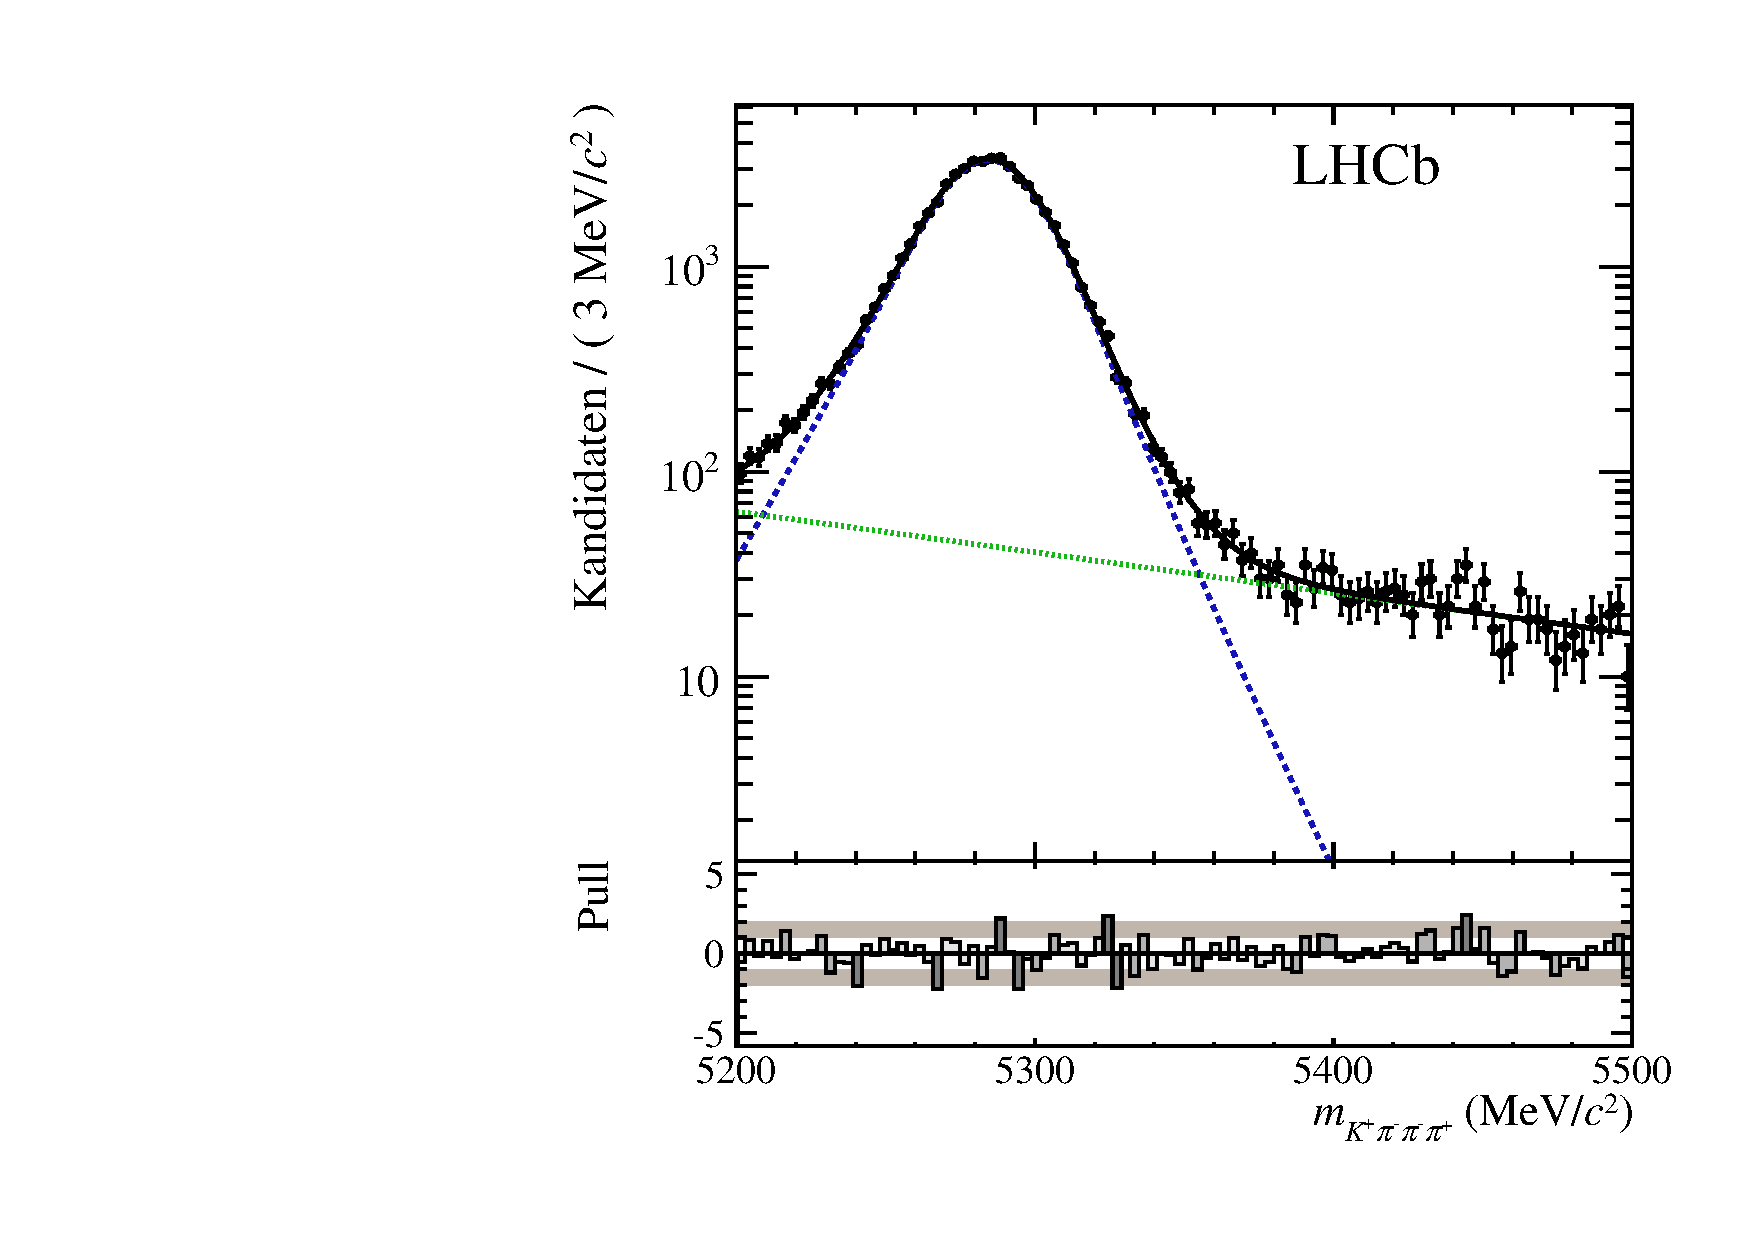
\includegraphics[width=0.45\textwidth]{fig/mass_OS_2011.pdf}
		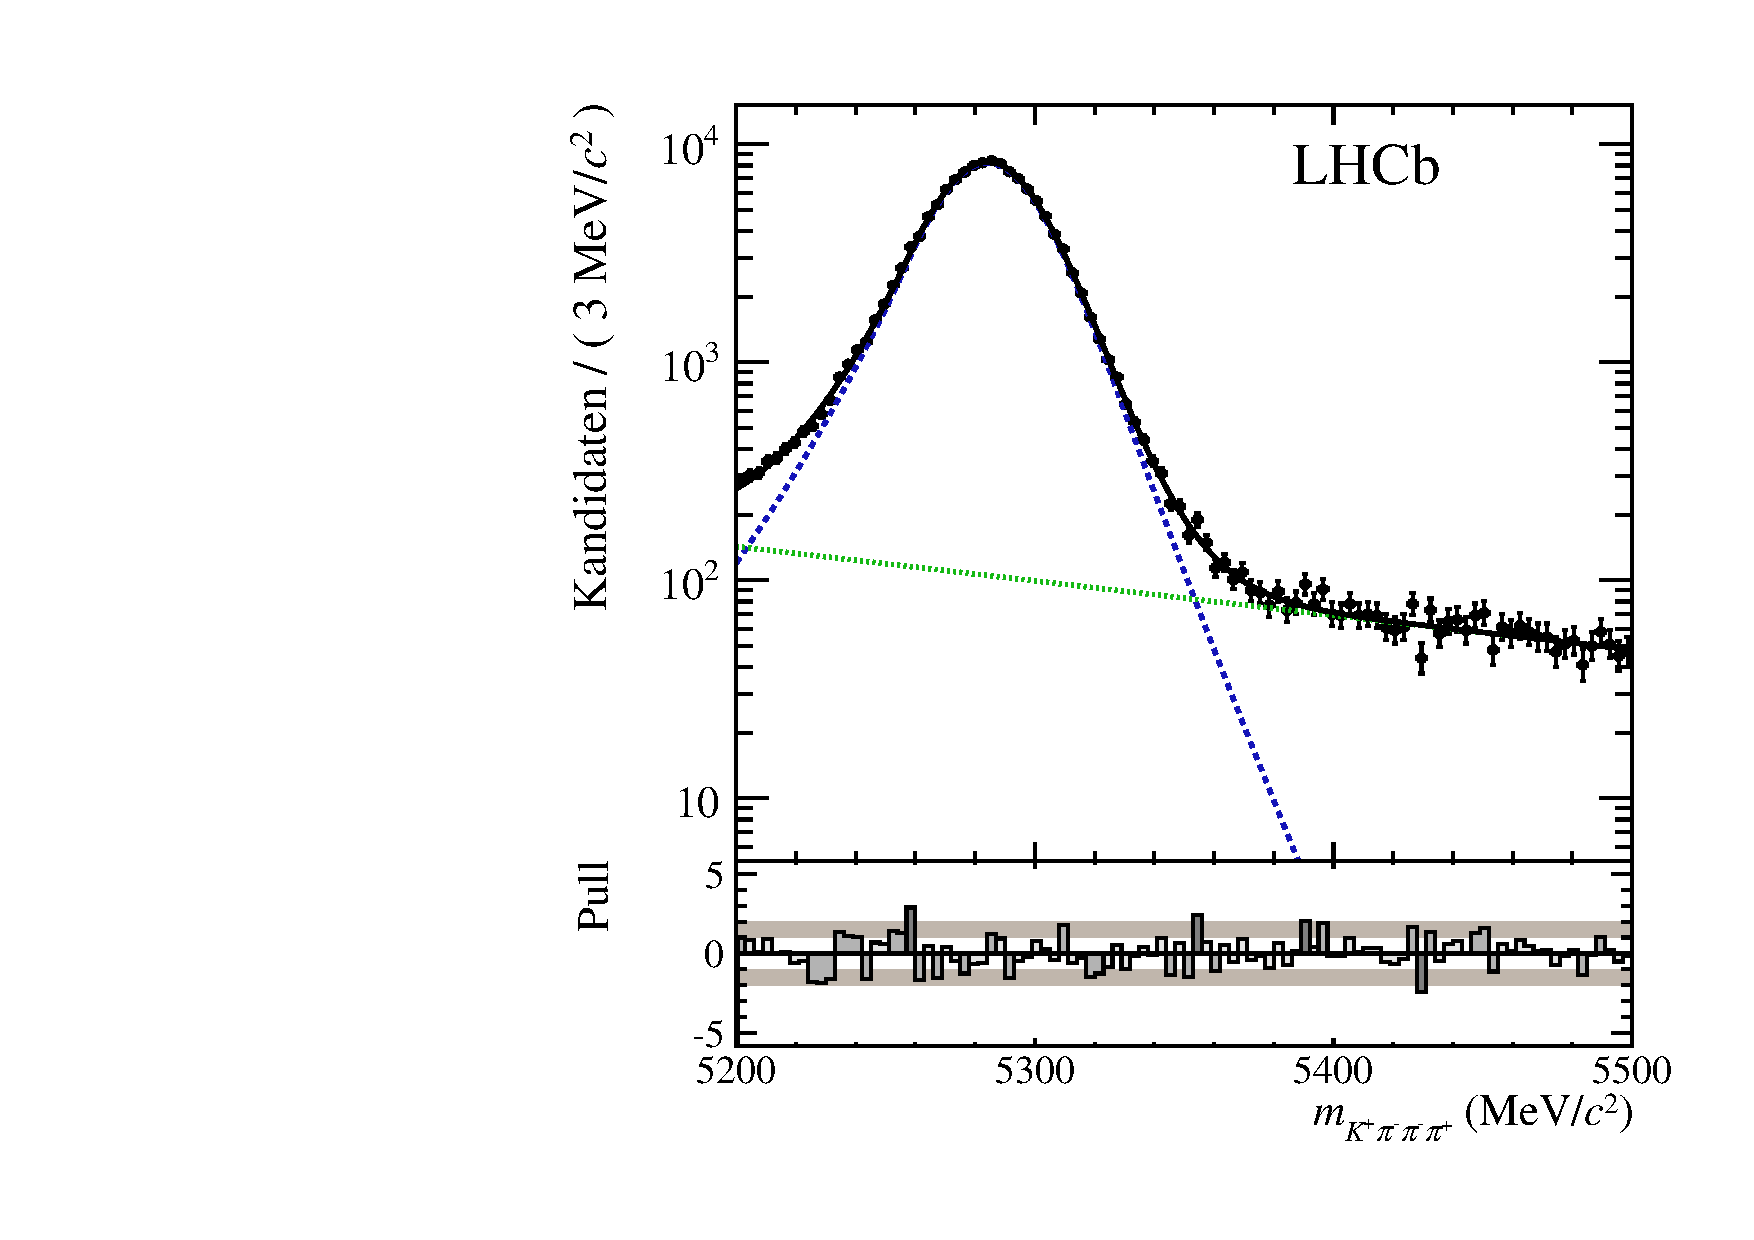
\includegraphics[width=0.45\textwidth]{fig/mass_OS_2012.pdf}
	\caption{Massenfit der \Bz-Mesonen für den \lhcb-Datensatz des Jahres \num{2011} (links) und \num{2012} (rechts) bei Signalkandidaten, die mit der OS Standard Kombination getaggt wurden. Im unteren Bereich der Plots ist die Abweichung der Datenpunkte von der angepassten Funktion in Einheiten der Standardabweichung gezeigt.}
	\label{fig:dmd_mass} 
\end{figure}
\begin{figure}[htbp]
	\centering
		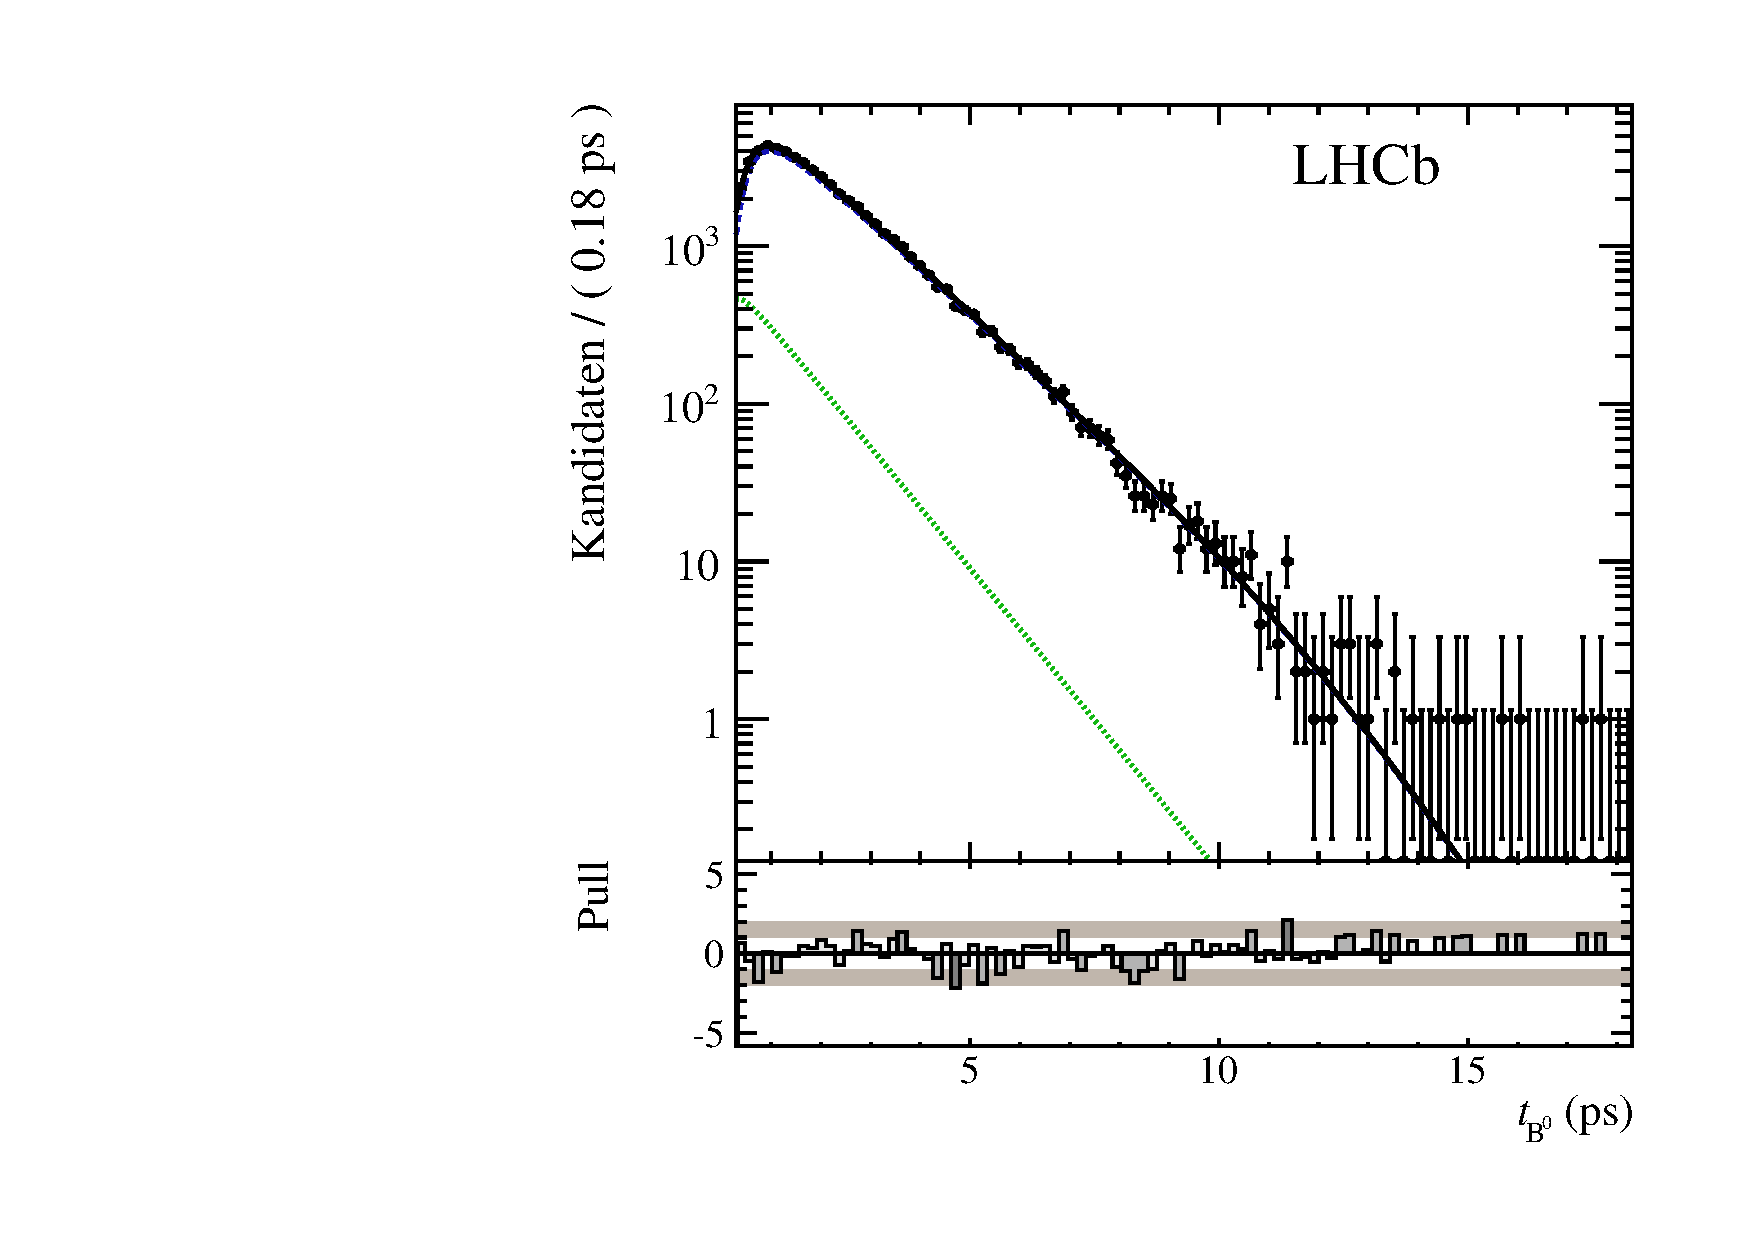
\includegraphics[width=0.45\textwidth]{fig/time_OS_2011.pdf}
		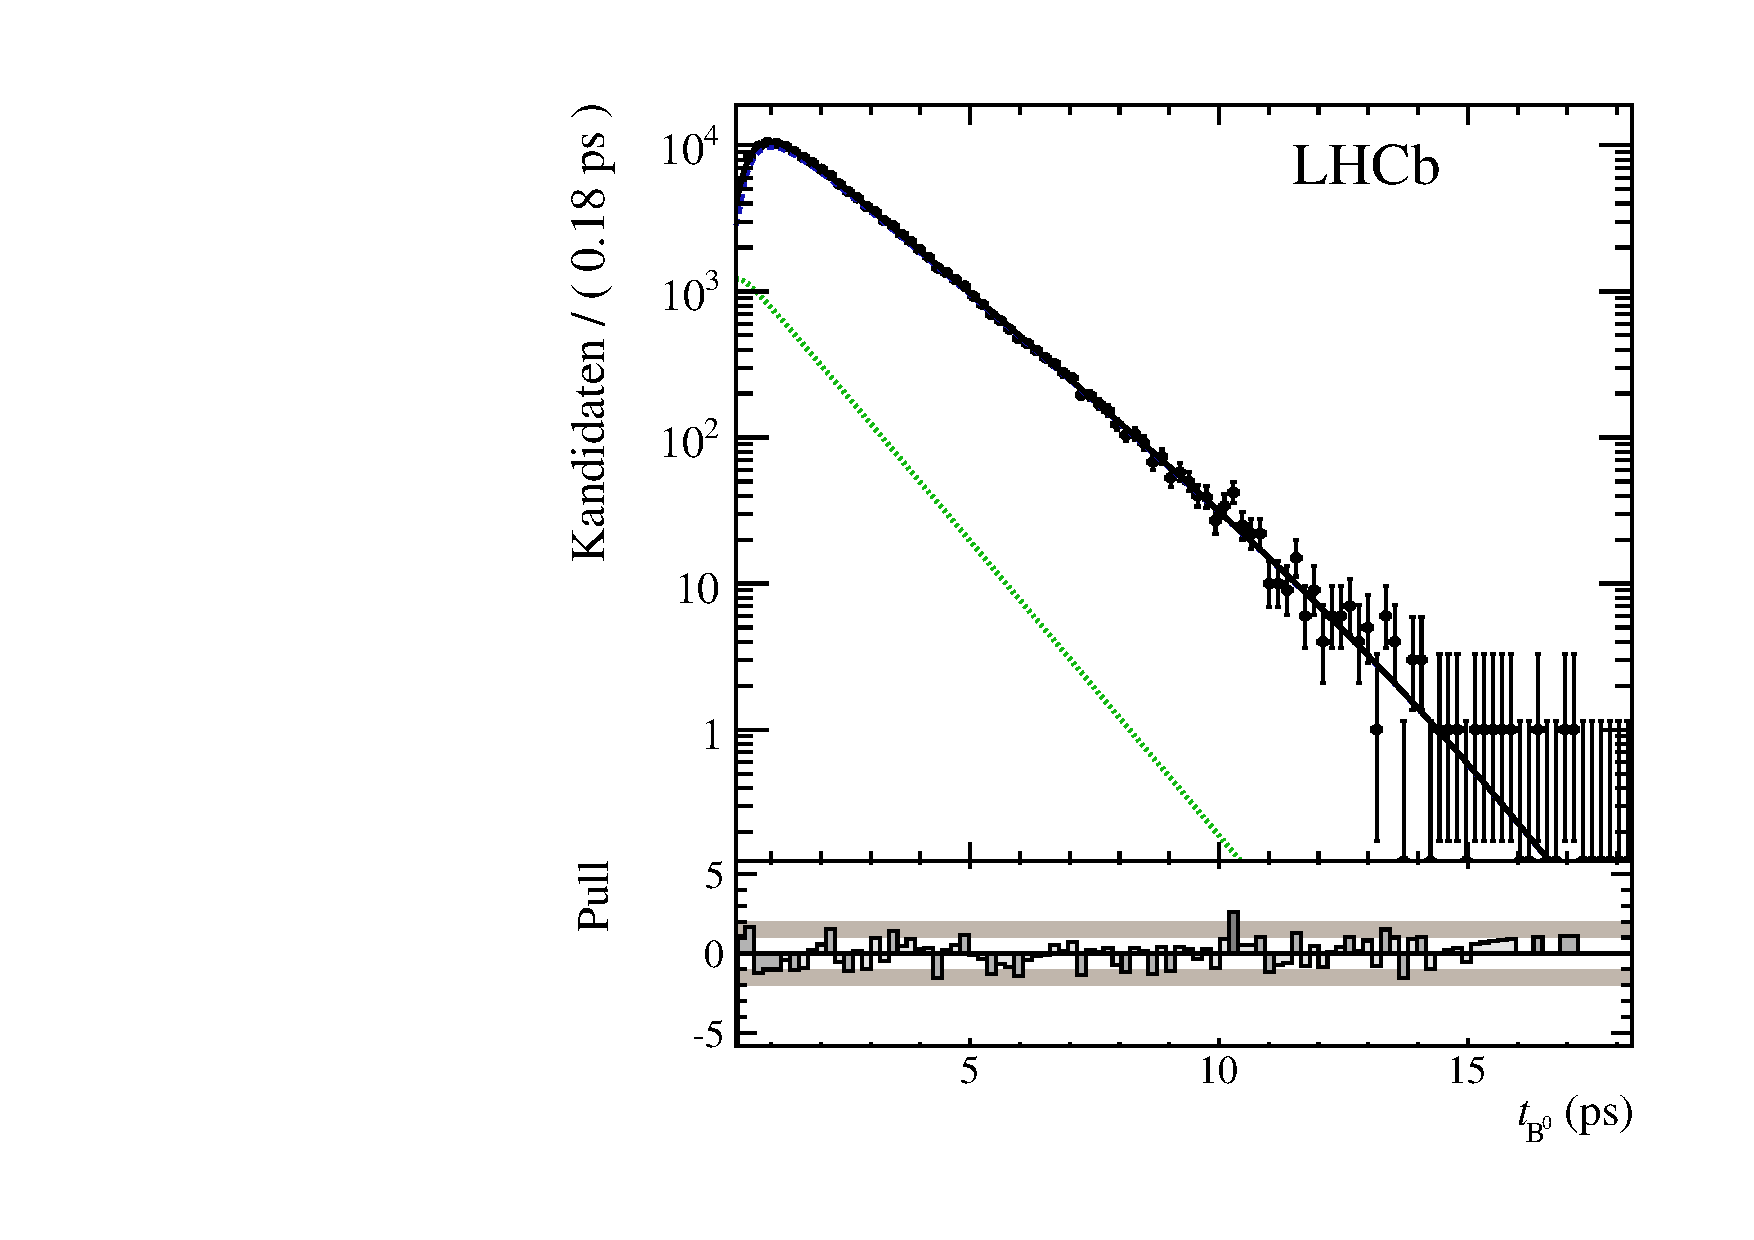
\includegraphics[width=0.45\textwidth]{fig/time_OS_2012.pdf}
	\caption{Lebenszeitfit der \Bz-Mesonen für den \lhcb-Datensatz des Jahres \num{2011} (links) und \num{2012} (rechts) bei Signalkandidaten, die mit der OS Standard Kombination getaggt wurden. Im unteren Bereich der Plots ist die Abweichung der Datenpunkte von der angepassten Funktion in Einheiten der Standardabweichung gezeigt.}
	\label{fig:dmd_time} 
\end{figure} 
\begin{figure}[htbp]
	\centering
		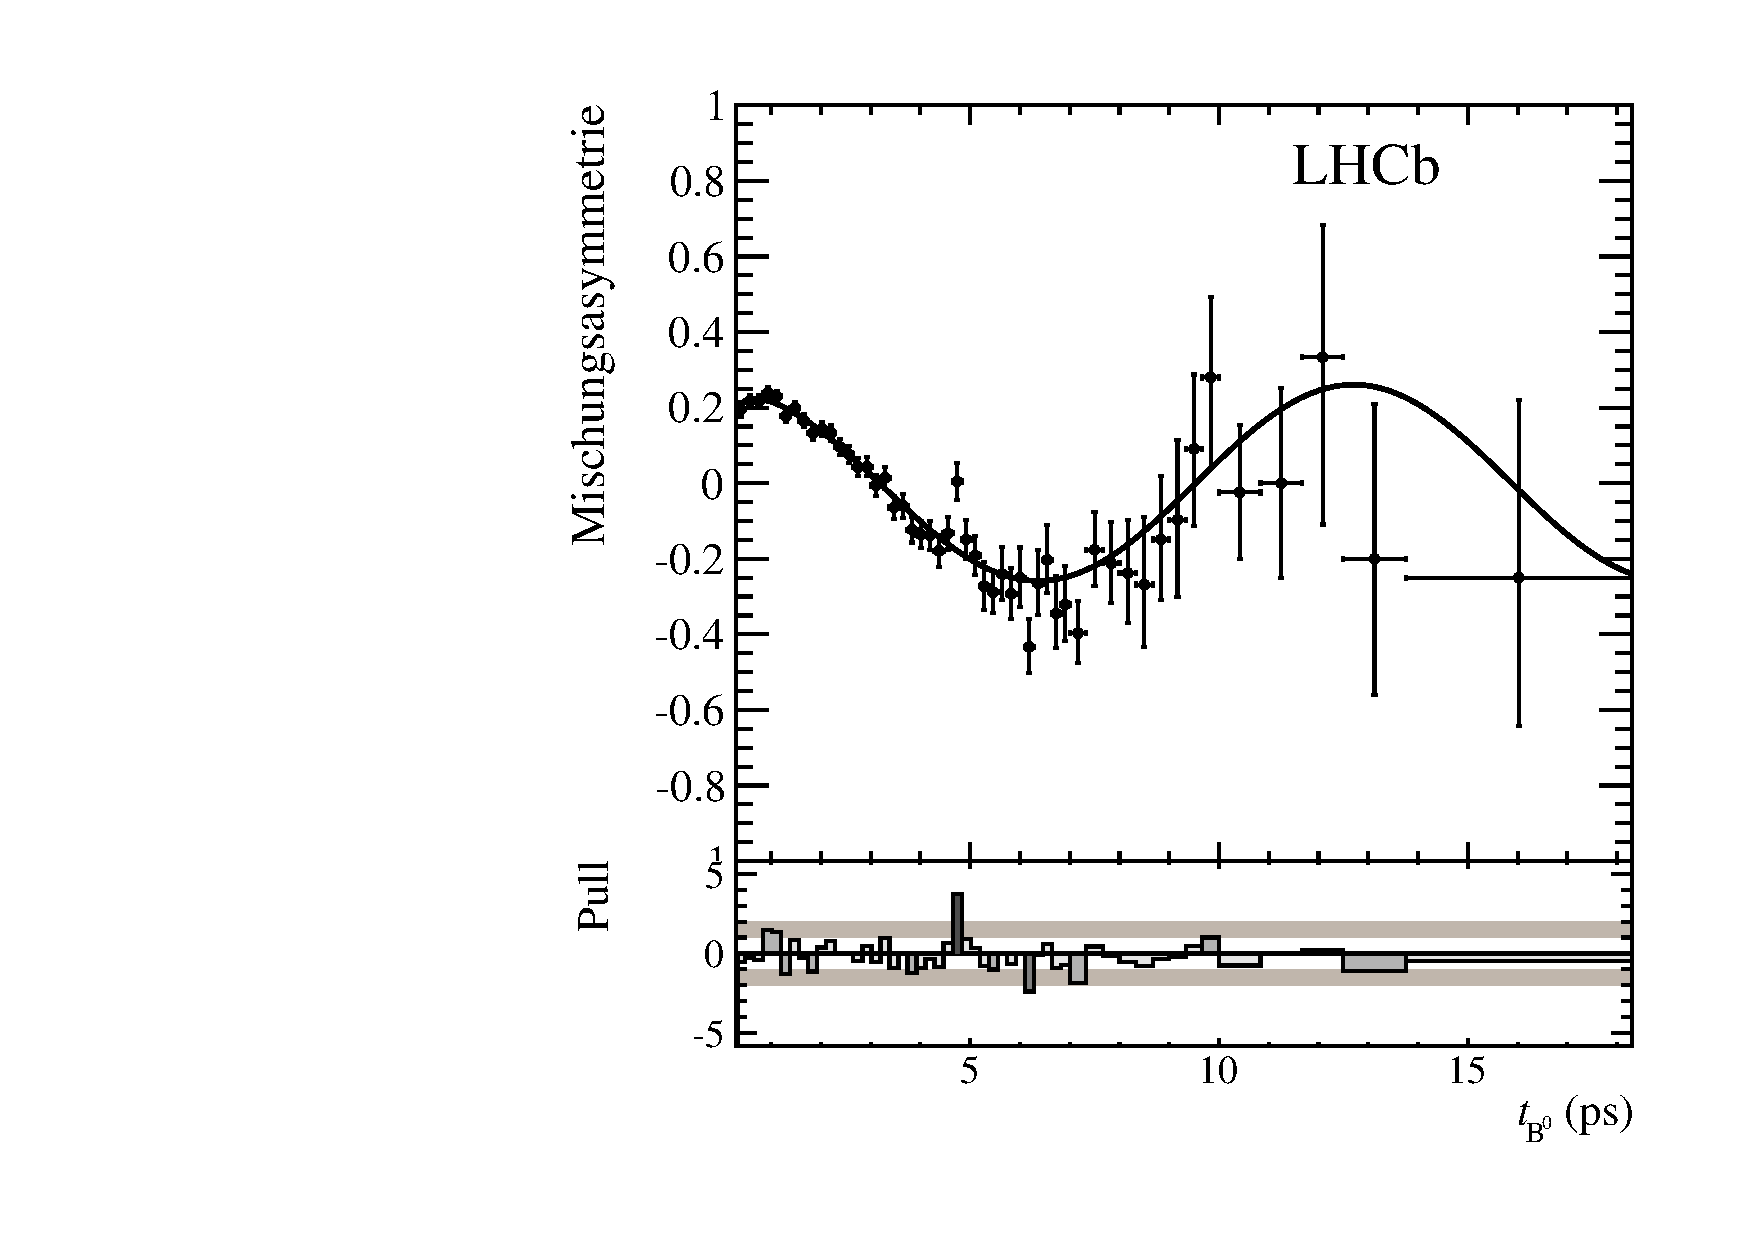
\includegraphics[width=0.45\textwidth]{fig/asymmetry_OS_2011.pdf}
		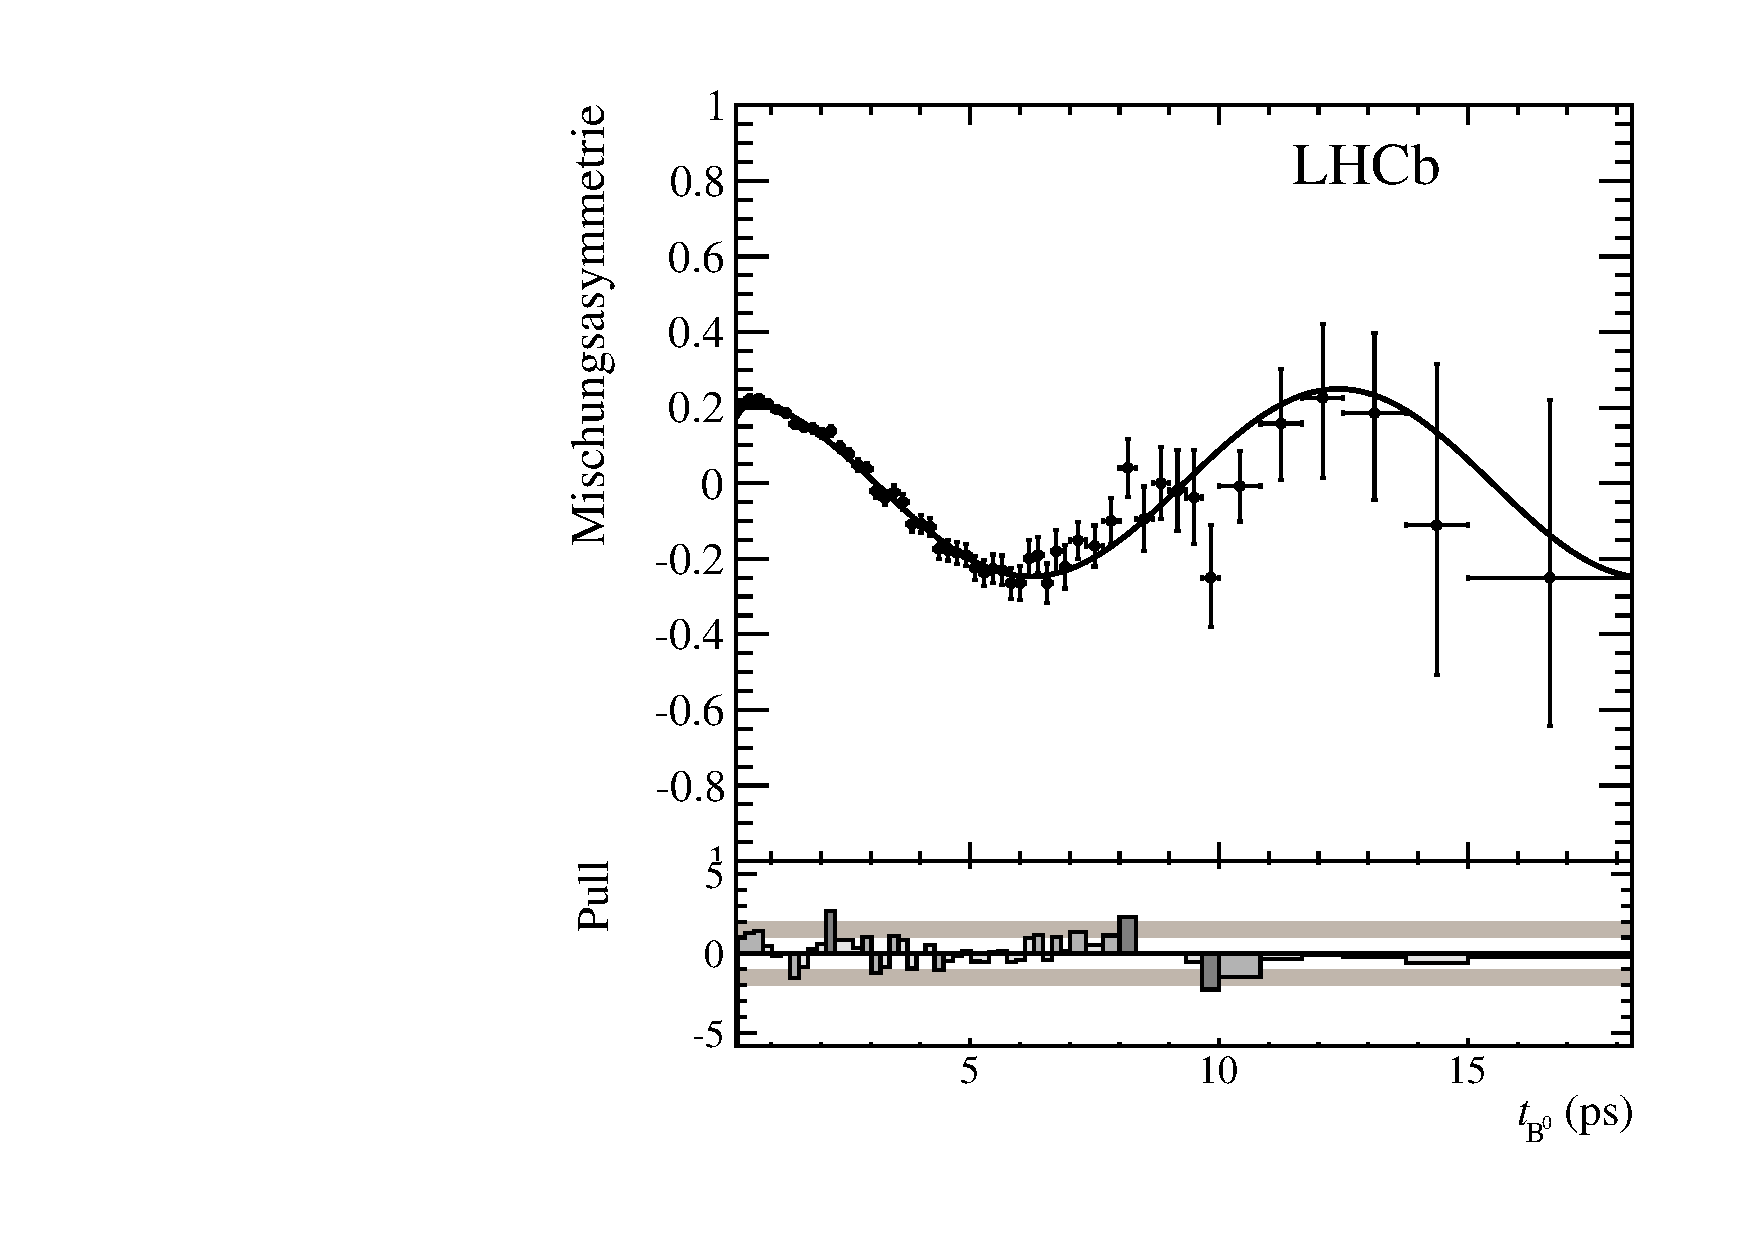
\includegraphics[width=0.45\textwidth]{fig/asymmetry_OS_2012.pdf}
	\caption{Mischungsasymmetrie \eqref{eq:mischung} der \Bz-Mesonen für den \lhcb-Datensatz des Jahres \num{2011} (links) und \num{2012} (rechts) bei Signalkandidaten, die mit der OS Standard Kombination getaggt wurden. Im unteren Bereich der Plots ist die Abweichung der Datenpunkte von der angepassten Funktion in Einheiten der Standardabweichung gezeigt.}
	\label{fig:dmd_asymmetry} 
\end{figure} 
Die statistischen Fehler auf \dmd sind unbeeinflusst von der Addition des unbekannten Offsets und sollen daher an dieser Stelle mit einer vorherigen Messung  auf dem Datensatz von \num{2011} \cite{dmd_messung} verglichen werden. Bei dieser wurden zur Bestimmung von \dmd die Kombination der Standard OS Kombination mit dem SS Pion Tagger verwendet. Diese sollen an dieser Stelle mit den statistischen Fehlern $\sigma_\text{stat}$ bei einer Messung nur mit der Standard OS Kombination verglichen werden, da bereits hier aufgrund der hohen Statistik für das Jahr \num{2012} zu erwarten ist, dass der statistische Fehler kleiner ist. Für diesen Vergleich sind in Tabelle \ref{tab:Reinheit} zunächst die getaggten Signal und Untergrundkandidaten zu sehen, sowie die sich daraus ergebende Reinheit $\frac{N_\text{Sig}}{N_\text{Bkg}}$.
\begin{table}[htbp]
	\centering
	\caption{Anzahl an Signal- und Untergrundkandidaten aus der \dmd-Messung aus \cite{dmd_messung} und der hier vorgestellten Analyse. Dabei ist zu beachten, dass in der hier vorgestellten Analyse nur die Standard OS Kombination verwendet wurde, während diese zuvor zusätzlich mit dem SS Pion Tagger kombiniert wurde.}
	\label{tab:Reinheit}
	\begin{tabular}{ccccc}
	\toprule
         			&\lhcb Analyse & \multicolumn{2}{c}{aktuelle Analyse} \\  
        Jahr der Datennahme & \num{2011}	 & \num{2011} & \num{2012} \\ 
        \midrule
       $N_\text{Sig}$	& $88200\pm500$ & $53305\pm242$ & $133075\pm^{381}_{380}$ \\ 
       $N_\text{Bkg}$	& $7170\pm^{350}_{390}$& $3470\pm^{94}_{93}$ & $8712\pm143$ \\ 
       \midrule
       $\frac{N_\text{Sig}}{N_\text{Bkg}}$ & $12{,}3\pm^{0{,}6}_{0{,}7}$ & $15{,}4\pm0{,}4$ & $15{,}3\pm0{,}3$  \\ 
       \bottomrule
	\end{tabular}
\end{table}
Bei dieser erkennt man, dass die aktuelle Selektion für beide Jahre bessere Ergebnisse für die Reinheit liefert. Die Analyse der von der OS Kombination getaggten Signalkandidaten in den \num{2012} aufgenommenen Daten sollte also bereits zu einem kleineren statistischen Fehler führen. Der Vergleich dieser Fehler ist in Tabelle \ref{tab:statFehler} zu sehen und man erkennt, dass die Erwartungen bezüglich einer statistisch größeren Genauigkeit bestätigt werden.
\begin{table}[htbp]
	\centering
	\caption{Statistischer Fehler $\sigma_\text{stat}$ auf die Größe \dmd. In der Analyse aus \num{2012} \cite{dmd_messung} wurde dieser extrahiert aus einer Kombination des SS Pion Taggers mit der OS Kombination. In der aktuellen Analyse wurde nur die OS Kombination verwendet.}
	\label{tab:statFehler} 
	\begin{tabular}{c|c|cccc}
	\toprule
         			&\lhcb Analyse & \multicolumn{3}{c}{aktuelle Analyse} \\  
        Jahr der Datennahme & \num{2011}	 & \num{2011} & \num{2012} & \num{2011}\&\num{2012}\\ 
        \midrule
       $\sigma_\text{stat}$	& \num{0{,}0061} & \num{0{,}0082} & \num{0{,}0055} & \num{0{,}0045} \\ 
       \bottomrule
	\end{tabular}
\end{table}

\section{Alternative Kalibrierung der OS Kombination}

Im Folgenden soll das in Abschnitt \ref{sec:kalibrierungDaten} erläuterte zweite Verfahren zur Kalibrierung des Flavour Taggings auf die OS Kombination angewendet werden. Dabei wird an dieser Stelle wegen der größeren Statistik der Datensatz aus dem Jahr \num{2012} verwendet. Es werden insgesamt \num{32} Kategorien der Wahrscheinlichkeit $P_\text{tag}(\bquarkbar)$ so gewählt, dass alle etwa die gleiche Statistik enthalten. Dabei gibt es kleine Unterschiede für die Kategorien für $P_\text{tag}(\bquarkbar)>0{,}5$ und $P_\text{tag}(\bquarkbar)<0{,}5$, da bei der Kategorisierung bei $P_\text{tag}(\bquarkbar)=0{,}5$ getrennt werden musste, um weiterhin zwischen \Bz- und \Bzb-Mesonen zu unterscheiden. In den Abbildungen \ref{fig:PBgetrennt1} und \ref{fig:PBgetrennt2} sind nun zunächst die Ergebnisse der linearen Kalibrierungen getrennt in den Bereichen $0<P_\text{tag}(\bquarkbar)<0{,}5$ und $0{,}5<P_\text{tag}(\bquarkbar)<1$ zu sehen. In Tabelle \ref{tab:PBgetrennt} sind die zugehörigen Ergebnisse dargestellt. Außerdem sieht man dort die Kalibrationsparameter $\Delta p_0$ und $\Delta p_1$, die die Taggingasymmetrie beschreiben. Diese berechnen sich hier nach
\begin{equation}
\Delta p_0=\left(1-p_0\right)-\overline{p_0}\hspace{1cm}\text{ und }\hspace{1cm}\Delta p_1=p_0-\overline{p_0}.
\end{equation}
Für die Zentralwerte $\widetilde{p_0}$ und $\widetilde{p_1}$ gilt
\begin{equation}
\widetilde{p_0}=\frac{\left(1-p_0\right)+\overline{p_0}}{2}\hspace{1cm}\text{ und }\hspace{1cm}\widetilde{p_1}=\frac{p_0+\overline{p_0}}{2}.
\end{equation}
 \begin{figure}[htbp]
	\centering
		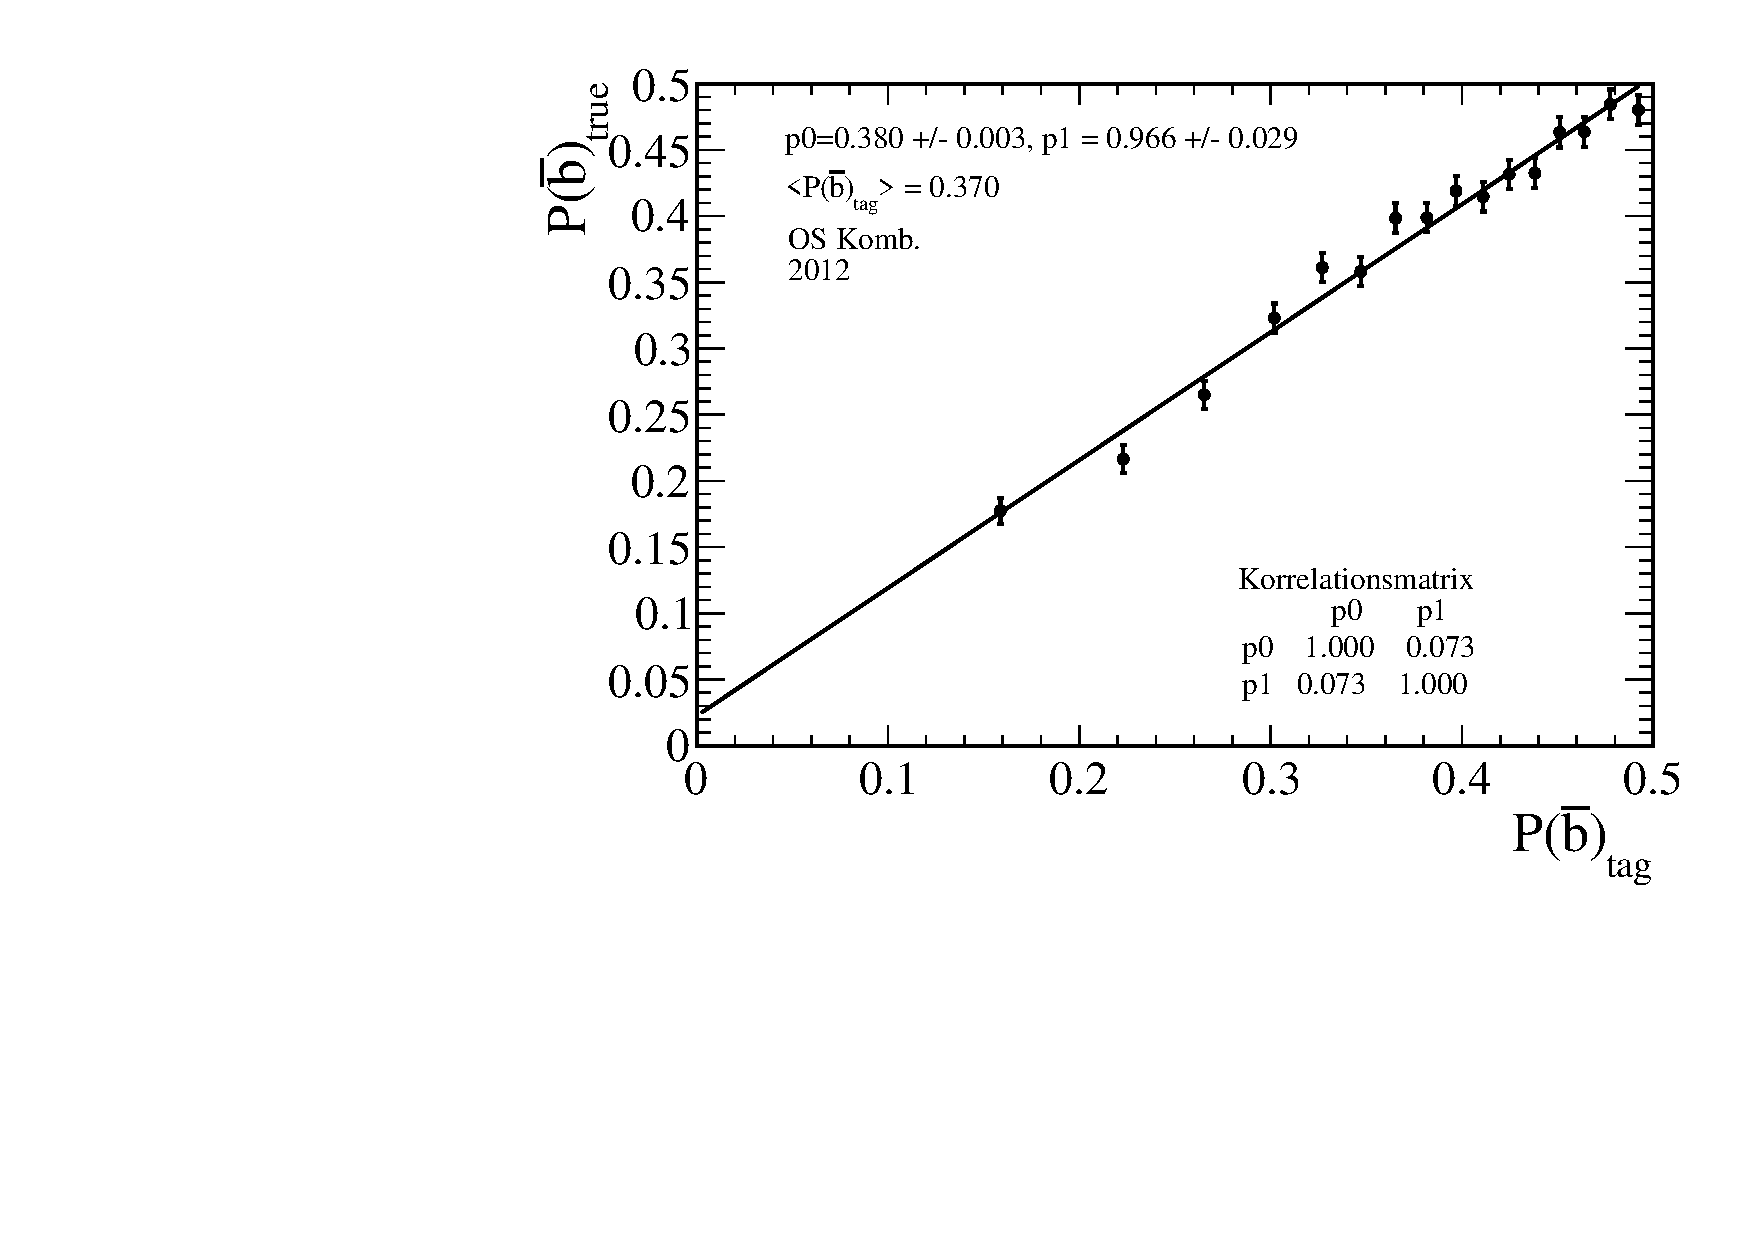
\includegraphics[width=0.75\textwidth]{fig/calibration_Bbar.pdf}
	\caption{Kalibrierung der OS Standard Kombination mit Wahrscheinlichkeiten $P(\bquarkbar)<0{,}5$ für \Bzb-Mesonen.}
	\label{fig:PBgetrennt1} 
\end{figure} 
 \begin{figure}[htbp]
	\centering
		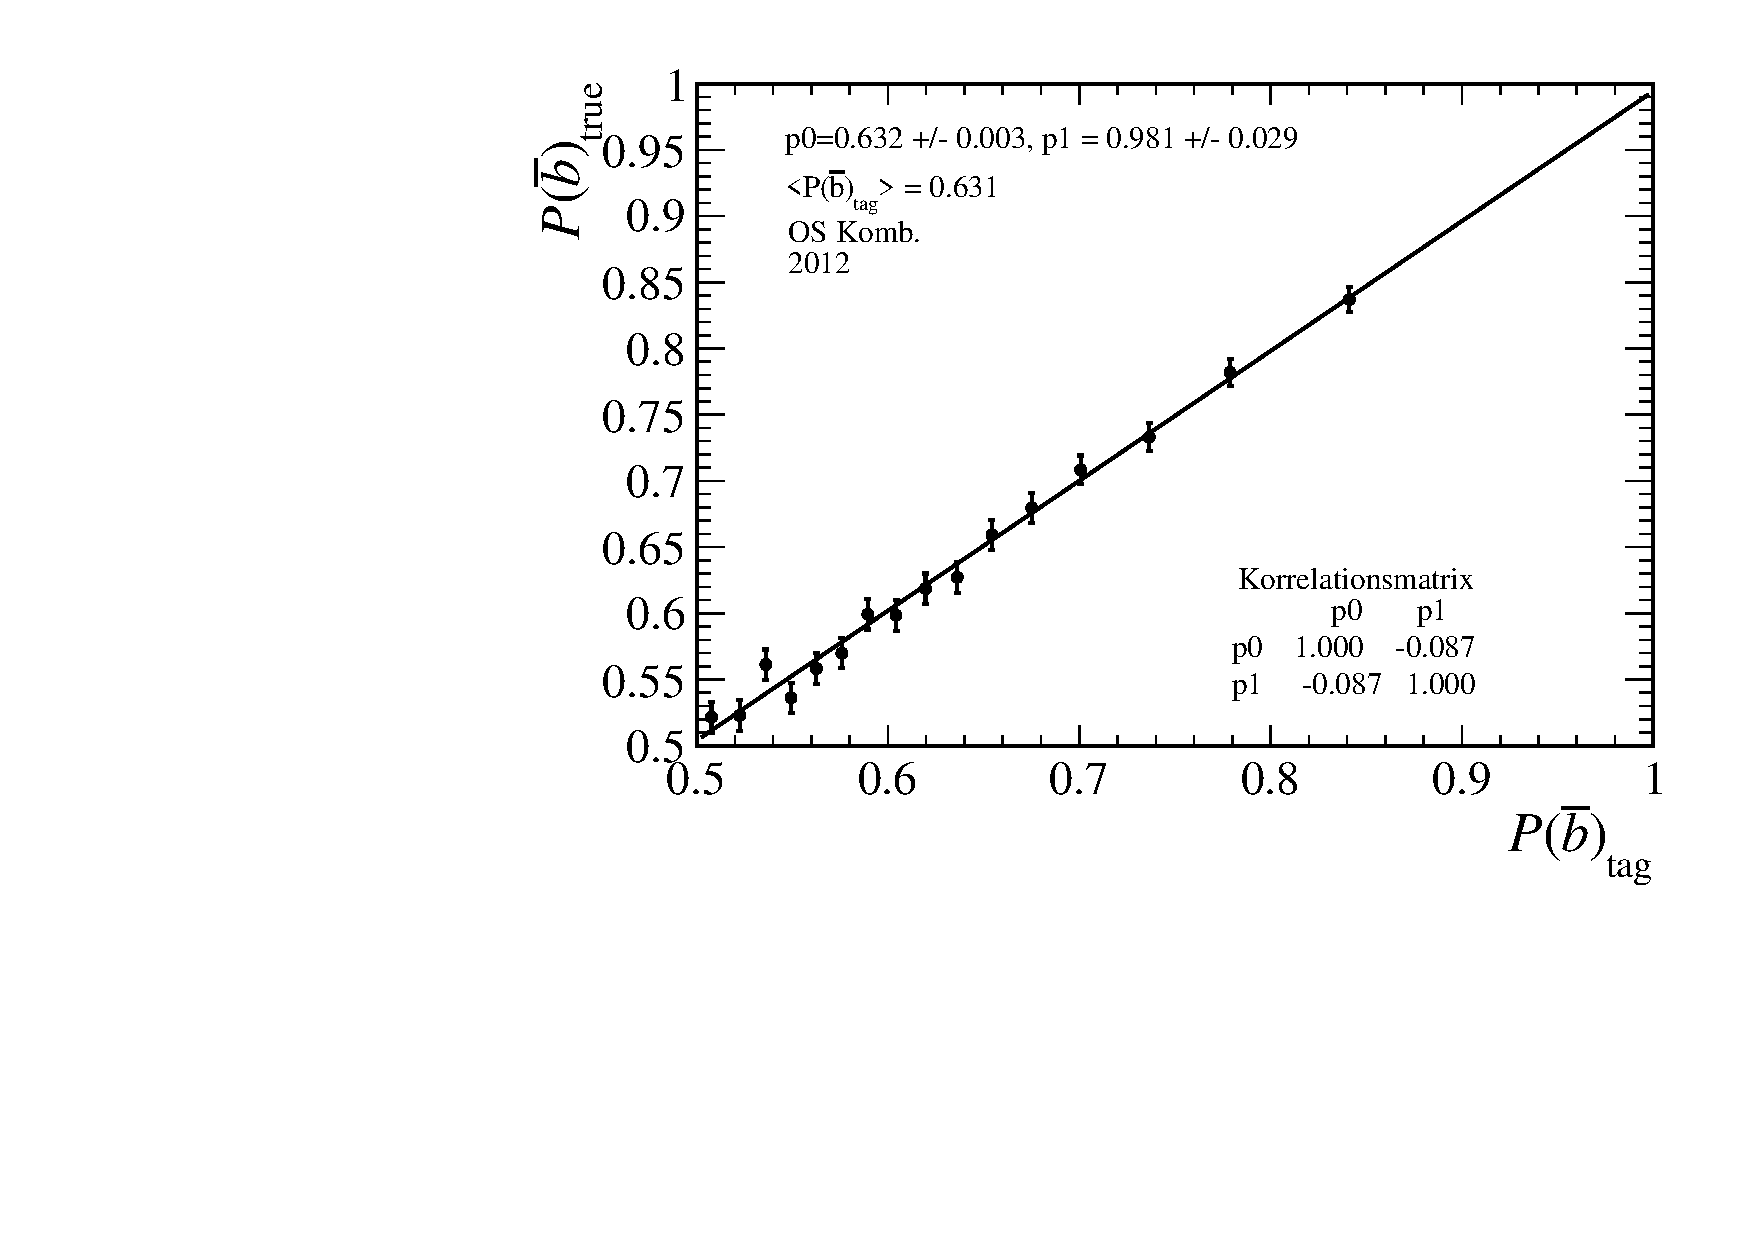
\includegraphics[width=0.75\textwidth]{fig/calibration_B.pdf}
	\caption{Kalibrierung der OS Standard Kombination mit Wahrscheinlichkeiten $P(\bquarkbar)>0{,}5$ für \Bz-Mesonen.}
	\label{fig:PBgetrennt2} 
\end{figure} 
\begin{table}[htbp]
	\centering
	\caption{Ergebnisse der linearen Kalibrierung der OS Standard Kombination mit Wahrscheinlichkeiten $P(\bquarkbar)$. Zum Vergleich die Ergebnisse der $(\eta,\omega)$-Kalibrierung.}
	\label{tab:PBgetrennt} 
	\begin{tabular}{c|ccc}
	\toprule
	 & $0<P_\text{tag}(\bquarkbar)<0{,}5$ & $0{,}5<P_\text{tag}(\bquarkbar)<1$ & $(\eta,\omega)$-Kalibrierung \\ 
	 \midrule
      $p_0$/$\overline{p_0}$  & $0{,}380\pm0{,}003$ & $0{,}632\pm0{,}003$ & - \\  
      $p_1$/$\overline{p_1}$ & $0{,}966\pm0{,}029$ & $0{,}981\pm0{,}029$ & - \\
      $\widetilde{p_0}$ & \multicolumn{2}{c}{$0{,}374\pm0{,}002$} &  $0{,}376\pm0{,}002$ \\
      $\widetilde{p_1}$ &  \multicolumn{2}{c}{$0{,}974\pm0{,}021$} &  $0{,}981\pm0{,}020$ \\
      $\Delta p_0$ & \multicolumn{2}{c}{$-0{,}012\pm0{,}004$} &  $0{,}018\pm0{,}003$ \\
      $\Delta p_1$ & \multicolumn{2}{c}{$-0{,}015\pm0{,}041$} &  $0{,}069\pm0{,}029$ \\ 
      \bottomrule
	\end{tabular}
\end{table}
Man sieht, dass die Ergebnisse für die Taggingasymmetrien dabei eindeutig von den Ergebnissen der Gesamtparametrisierung aus der $(\eta,\omega)$-Kalibrierung abweichen. Dies ist hier zu erwarten, da die Taggingasymmetrien für die \enquote{echten} initialen \B-Mesonen definiert sind. Bei der Unterscheidung für die hier gezeigte Kalibrierung, steht jedoch nur die fehlerbehaftete Tagentscheidung zur Verfügung. Dies lässt sich auf Monte Carlo Daten bestätigen, wo der anfängliche Flavour der \B-Mesonen bekannt ist. In Tabelle \ref{tab:mcgetrennt} wurde dazu zunächst eine komplette Kalibrierung mit einem Zeitfit durchgeführt. Aus dieser Kalibrierung erhält man die Parameter $\widetilde{p_0}$, $\widetilde{p_1}$, $\Delta p_0$ und $\Delta p_1$. Außerdem lässt sich die Kalibrierung, wie auf Daten, getrennt nach der Tagentscheidung, für getaggte \Bz- und \Bzb-Mesonen durchführen, um so die Parameter $p_0$, $\overline{p_0}$, $p_1$ und $\overline{p_1}$ zu erhalten. Dabei sieht man wiederum die qualitativ gleichen Unterschiede wie in Tabelle \ref{tab:PBgetrennt}. Als weitere Möglichkeit lässt sich auf Monte-Carlo nun allerdings auch nach dem in Abschnitt \ref{sec:mckalibrierung} beschriebenen Verfahren für \Bz- und \Bzb-Mesonen getrennt kalibrieren, wobei allerdings nicht nach der Tagentscheidung, sondern dem \enquote{wahren} Anfangszustand unterschieden wird.
\begin{table}[htbp]
	\centering
	\small
	\caption{Vergleich der linearen Kalibrierungsparameter bei der Beschreibung der Taggingasymmetrie. In der ersten Zeile ist die Größe angegeben, nach der für die Kalibrierung getrennt wurde.}
	\label{tab:mcgetrennt} 
	\begin{tabular}{c|ccccc}
	\toprule
	 & \multicolumn{2}{c}{Tag $d$} & \multicolumn{2}{c}{\enquote{wahrer} Flavour} & Gesamtfit \\
	 & \Bzb & \Bz & \Bzb & \Bz & \Bzb \& \Bz \\ 
	 \midrule
      $p_0$/$\overline{p_0}$  & $0{,}353\pm0{,}011$ & $0{,}349\pm0{,}011$ & $0{,}348\pm0{,}007$ & $0{,}353\pm0{,}007$ & - \\  
      $p_1$/$\overline{p_1}$ & $0{,}933\pm0{,}116$ & $0{,}772\pm0{,}122$ & $0{,}876\pm0{,}077$ & $0{,}916\pm0{,}078$ & - \\
      $\widetilde{p_0}$ & \multicolumn{2}{c}{$0{,}351\pm0{,}008$} & \multicolumn{2}{c}{$0{,}351\pm0{,}005$} &  $0{,}350\pm0{,}008$ \\
      $\widetilde{p_1}$ &  \multicolumn{2}{c}{$0{,}853\pm0{,}084$} & \multicolumn{2}{c}{$0{,}896\pm0{,}054$} & $0{,}828\pm0{,}082$ \\
      $\Delta p_0$ & \multicolumn{2}{c}{$-0{,}004\pm0{,}015$} & \multicolumn{2}{c}{$0{,}005\pm0{,}010$} & $0{,}005\pm0{,}009$ \\
      $\Delta p_1$ & \multicolumn{2}{c}{$-0{,}161\pm0{,}168$} & \multicolumn{2}{c}{$0{,}040\pm0{,}110$} & $0{,}029\pm0{,}052$ \\ 
      \bottomrule
	\end{tabular}
\end{table}
Vergleicht man nun die sich ergebenden Taggingasymmetrien zwischen den beiden getrennten Kalibrierungen jeweils mit der Kalibrierung aus dem Gesamtfit, sieht man, dass die Parameter für die Trennung nach \enquote{wahren} Produktionsflavour eine gute Übereinstimmung zeigt, während bei der Trennung nach der Tagentscheidung $d$ hier ähnliche Effekte wie zuvor zu beobachten sind. 

  % !TEX root = main.tex
\chapter{Zusammenfassung und Ausblick}

Im Zuge der vorgestellten Arbeit wurden im Bereich des Flavour Taggings am \lhcb-Experiment verschiedene Tagger untersucht. Dabei wurden zunächst auf der Opposite Side für die OS Kombination, den OS Charm Tagger und den OS Kaon nnet Tagger die Kalibrierung der mistag-Wahrscheinlichkeiten $\eta$ in Bezug auf die wahren mistag-Wahrscheinlichkeiten $\omega$ überprüft.\\
Weiter wurde dieser Zusammenhang auch auf der Same Side für drei Tagger überprüft. Der SS Pion Tagger wies dabei deutlich stärkere Abweichungen von einer idealen Kalibration auf als die Tagger der Opposite Side. Für die beiden weiteren Tagger, den SS Proton und den SS Pion BDT Tagger, zeigten sich auch Abweichungen vom ideal kalibrierten Fall. Allerdings lag der Fokus hier weniger auf der Gegenprobe der Kalibrierung, sondern vielmehr auf der grundsätzlichen Funktionalität beider Tagger, da es sich um Neuentwicklungen handelt. Nach einigen Problemen bei der Entwicklung, konnte in dieser Arbeit diese Funktionalität das erste Mal bestätigt werden. Außerdem ließ sich hier die effektive Taggingeffizienz $\varepsilon D^2$ des SS Pion Taggers und  seines zukünftigen Nachfolgers, dem SS Pion BDT Tagger, vergleichen. Dabei ergab sich für den SS Pion BDT eine etwa \SI{0{,}6}{\%} höhere effektive Taggingeffizienz.\\
Da sowohl der SS Proton als auch die beiden Pionen Tagger den Hadronisierungsprozess des gleichen Quarks untersuchen, wurden hier außerdem erste Untersuchungen einer möglichen Korrelation der verschiedenen Tagger auf der Same Side untersucht. Eine quantitative Aussage ist an dieser Stelle noch nicht möglich. Die beobachteten Korrelation zwischen den mistag-Verteilungen und den Taggingentscheidungen sind jedoch größer zwischen dem SS Proton und dem SS Pion BDT Tagger als zwischen dem SS Proton und dem SS Pion Tagger. \\ 
\\
Weiterhin wurde bei der Kalibrierung der Tagger die Mischungsfrequenz $\dmd$  der neutralen \B-Mesonen bestimmt. Diese Messung wurde blind durchgeführt. Es konnte jedoch gezeigt werden, dass der statistische Fehler auf diese Observable mit dem \num{2012} bei \lhcb aufgenommenen Datensatz nur bei Verwendung der durch die OS Kombination getaggten Ereignisse bereits kleiner ist als bei einer älteren Analyse auf dem \num{2011} aufgenommenen Datensatz, bei der eine Kombination aus der OS Kombination und dem SS Pion Tagger verwendet wurde. Außerdem zeigt die neue Selektion auf den Datensätzen beider Jahre eine bessere Reinheit. \\
\\
Zur Kalibrierung des Flavour Taggings wird aktuell eine Methodik angewendet, bei der die mistag-Wahrscheinlichkeiten $\eta$ auf true-mistag-Wahrscheinlichkeiten $\omega$ kalibriert werden. Hier wurde eine alternative Herangehensweise vorgestellt, bei der zwischen \Bz- und \Bzb-Mesonen unterschieden werden kann. Dabei werden die mistag-Wahrscheinlichkeiten $\eta$ in anschaulichere $P(\bquarkbar)$, die Wahrscheinlichkeit, dass es sich bei einem Teilchen um ein \Bz-Meson handelt, umgerechnet. Dieses Verfahren bietet sich auch in hinsichtlich dessen an, dass die Tagger selbst intern mit der Wahrscheinlichkeit $P(\bquarkbar)$ rechnen. Da auf Daten jedoch nur über den Tag $d$ zwischen \Bz- und \Bzb-Meson unterschieden werden kann, und der \enquote{wahre} Flavour nicht bekannt ist, sind die Parameter $\Delta p_0$ und $\Delta p_1$, die eine mögliche Taggingasymmetrie berücksichtigen, in diesem Verfahren zunächst nicht korrekt bestimmbar.\\
\\
Die Ergebnisse der Prüfung der Kalibrierung der verschiedenen Tagger auf dem Kanal \BdToDpi werden in die Bestimmung der Systematiken der Standard Kalibration der Flavour Tagging Gruppe eingehen. Daneben müssen für die hier vorgestellten Parameter allerdings auch noch die systematische Unsicherheiten bestimmt werden. Außerdem sind weitere Proben auf einem kombinierten Datensatz aus den Jahren \num{2011} und \num{2012} möglich. 

\backmatter
 % \nocite{*}
  \printbibliography

\newpage
\pagestyle{empty}
% !TEX root = main.tex
\section*{Danksagung}

Zuallererst möchte ich Herrn Professor Dr. Bernhard Spaan dafür danken, dass er mir ein so interessantes Thema für meine Massenarbeit zur Verfügung gestellt hat und ich die Möglichkeit hatte aktiv an einem internationalen Forschungsprojekt mitzuarbeiten. Ebenfalls danke ich Priv.-Doz. Dr. Reiner Klingenberg dafür, dass er sich als Zweitgutachter meiner Masterarbeit zur Verfügung gestellt hat.\\
Meinen Masterkollegen Janine, Vanessa, Daniel, Philip, Timon und Tobias danke ich für die für die vielen angenehmen Stunden während der Zeit der Masterarbeit im Büro, auf Reisen zu Konferenzen oder bei einem Kaffee oder Tee in kleinen Pausen. Auch wäre ich sicher nicht so gut durch die acht vorangegangen Semester gekommen, wenn mich nicht Daniel, Mathis, David oder Dominik in diversen Vorlesungen begleitet hätten und wir viele Übungsblätter gemeinsam gerechnet hätten.\\
In der Arbeitsgruppe möchte ich zunächst Ulrich, mit dem ich direkt zusammengearbeitet habe, für seine Unterstützung meinen besonderen Dank aussprechen. Er stand mir bei jeder Frage mit hilfreichen Antworten und Anregungen zur Seite und hat mir hervorragend durch das Jahr meiner Massenarbeit geholfen. Weiter standen mir Christophe und Julian bei Herausforderungen während meiner Masterarbeit immer für anregende Diskussionen zur Verfügung; auch dafür einen großen Dank an dieser Stelle. Ebenso gilt mein Dank für Hilfestellungen an verschiedensten Stellen Florian, Frank, Ramon und Robert. Für die Hilfe in bürokratischen Angelegenheiten danke ich außerdem Frau Stickel, ohne die manch ein Antrag sicher deutlich mehr Arbeit bedeutet hätte.\\
Weiterhin danke ich an dieser Stelle allen Mitglieder des Lehrstuhls E5 für die sehr erfreuliche Zusammenarbeit in einer angenehmen Arbeitsatmosphäre und die erfrischenden Diskussionen, die sich unter Anderem in gemeinsamen Mittagspausen ergeben haben. \\ 
Für das Korrekturlesen meiner Arbeit danke ich außerdem Moritz und Tobias, der mir außerdem mit seiner großen Erfahrung während gemeinsamer Laufeinheiten immer wieder interessante Ansätze liefern konnte.\\
Abschließend möchte ich Thomas für die schönen Ablenkungen beim Fußball danken, ob es als Trainer- oder Spielerkollege war oder auch bei einer Würfelrunde gemeinsam mit Tobias, Jens und Julian nach dem Training. Außerdem gilt mein Dank natürlich meinen Eltern sowie meinen beiden Brüdern, die mir mein Studium erst ermöglicht haben und mich durchgehend nach Kräften unterstützt haben.

\newpage
% !TEX root = main.tex
\section*{Eidesstattliche Versicherung}
\vspace*{1cm}
\noindent
Ich versichere hiermit an Eides statt, dass ich die vorliegende Masterarbeit mit dem Titel \enquote{Kalibrierung des Flavour Taggings im Kanal $\Bz\to\Dm\pip$ am \lhcb- Experiment} selbst\"andig und ohne unzul\"assige fremde Hilfe erbracht habe. Ich habe keine anderen als die angegebenen
Quellen und Hilfsmittel benutzt sowie w\"ortliche und sinngem\"a\ss e Zitate kenntlich gemacht.
Die Arbeit hat in gleicher oder \"ahnlicher Form noch keiner Pr\"ufungsbeh\"orde vorgelegen.
\vspace*{1cm}
\ \\
\ \\
\line(1,0){150} \hfill \line(1,0){150}\\
Ort, Datum \hfill Unterschrift \hspace*{3cm}
\vspace*{1.5cm}

\subsection*{Belehrung}
Wer vors\"atzlich gegen eine die T\"auschung \"uber Pr\"ufungsleistungen betreffende Regelung einer Hochschulpr\"ufungsordnung
verst\"o\ss t handelt ordnungswidrig. Die Ordnungswidrigkeit kann mit einer Geldbu\ss e von bis zu \SI{50.000,00}{\euro} geahndet werden. Zust\"andige Verwaltungsbeh\"orde f\"ur die Verfolgung und Ahndung von Ordnungswidrigkeiten ist
der Kanzler/die Kanzlerin der Technischen Universit\"at Dortmund. Im Falle eines mehrfachen oder sonstigen schwerwiegenden T\"auschungsversuches kann der Pr\"ufling zudem exmatrikuliert werden (\S\ 63 Abs. 5 Hochschulgesetz - HG - ).\\
\ \\
Die Abgabe einer falschen Versicherung an Eides statt wird mit Freiheitsstrafe bis zu 3 Jahren oder mit Geldstrafe bestraft.\\
\ \\
Die Technische Universit\"at Dortmund wird ggf. elektronische Vergleichswerkzeuge (wie z.B. die Software ''turnitin'') zur \"Uberpr\"ufung von Ordnungswidrigkeiten in Pr\"ufungsverfahren nutzen.\\
\ \\
Die oben stehende Belehrung habe ich zur Kenntnis genommen.
\vspace*{1cm}
\ \\
\ \\
\line(1,0){150} \hfill \line(1,0){150}\\
Ort, Datum \hfill Unterschrift \hspace*{3cm}
\vspace*{\fill}
\end{document}

